        %%******************************************%%
        %%                                          %%
        %%        Modello di tesi di laurea         %%
        %%            di Andrea Giraldin            %%
        %%                                          %%
        %%             2 novembre 2012              %%
        %%                                          %%
        %%******************************************%%

\begin{document}
    \frontmatter
    \begin{titlepage}
    \begin{center}
        \begin{LARGE}
            \textbf{\myUni}\\
        \end{LARGE}

        \vspace{10pt}

        \begin{Large}
            \textsc{\myDepartment}\\
        \end{Large}

        \vspace{10pt}

        \begin{large}
            \textsc{\myFaculty}\\
        \end{large}

        \vspace{30pt}
        \begin{figure}[htbp]
            \centering
            
\includegraphics[height=6cm]{unipd-logo}
        \end{figure}
        \vspace{30pt}

        \begin{LARGE}
            \textbf{\myTitle}\\
        \end{LARGE}

        \vspace{10pt}

        \begin{large}
            \textsl{\myDegree}\\
        \end{large}

        \vspace{40pt}

        \begin{large}
            \begin{flushleft}
                \textit{Relatore}\\
                \vspace{5pt}
                \profTitle\ \myProf
            \end{flushleft}

            % You can tweak the spacing to have professor and student names on the same line
            % useful if the page is broken by a long thesis title and you need more space
            % \vspace{-52pt}

            \begin{flushright}
                \textit{Laureando}\\
                \vspace{5pt}
                \myName
            \end{flushright}
        \end{large}

        \vspace{40pt}

        \line(1, 0){338} \\
        \begin{normalsize}
            \textsc{Anno Accademico \myAA}
        \end{normalsize}
    \end{center}
\end{titlepage}

    \clearpage
\phantomsection
\thispagestyle{empty}

\hfill
\vfill

\noindent\myName: \textit{\myTitle,}
\myDegree,
\textcopyright\ \myTime.

    %\cleardoublepage
\phantomsection
\thispagestyle{empty}
\pdfbookmark{Dedica}{Dedica}

\vspace*{3cm}

\begin{center}
    Lorem ipsum dolor sit amet, consectetuer adipiscing elit. \\ \medskip
    --- Oscar Wilde
\end{center}

\medskip

\begin{center}
    Dedicato a ...
\end{center}

    \cleardoublepage
\phantomsection
\pdfbookmark{Sommario}{Sommario}
\begingroup
\let\clearpage\relax
\let\cleardoublepage\relax
\let\cleardoublepage\relax

\chapter*{Sommario}

Il presente documento descrive il lavoro svolto durante il periodo di stage avvenuto presso l'azienda RiskApp Srl. \\

\noindent Il progetto di stage consisteva nella realizzazione di un'applicazione mobile per la gestione di \gls{meetingnote}\glsoccur, rivolta ad un sotto insieme di utenti che svolgono il loro lavoro in mobilità. \\


\noindent Gli obbiettivi da raggiungere sono stati molteplici. Tra quelli obbligatori erano presenti lo sviluppo della UI e delle funzionalità di base: login, creazione, modifica, eliminazione e visualizzazione di una \gls{meetingnote}\glsoccur.\\
Mentre tra quelli opzionali, l'integrazione di \gls{openai}\glsoccur per automatizzare il processo di creazione menzionato sopra, l'implementazione dei test per la verifica e validazione ed infine l'effettuazione del deploy dell'applicazione sulle piattaforme \emph{Android} e \emph{iOS}.\\

%\vfill

%\selectlanguage{english}
%\pdfbookmark{Abstract}{Abstract}
%\chapter*{Abstract}

%\selectlanguage{italian}

\endgroup

\vfill

    \cleardoublepage
\phantomsection
\pdfbookmark{Ringraziamenti}{ringraziamenti}

\begin{flushright}{
    \slshape
    ``Life is really simple, but we insist on making it complicated''} \\
    \medskip
    --- Confucius
\end{flushright}


\bigskip

\begingroup
\let\clearpage\relax
\let\cleardoublepage\relax
\let\cleardoublepage\relax

\chapter*{Ringraziamenti}

\noindent \textit{Innanzitutto, vorrei esprimere la mia gratitudine al Prof. \myProf, relatore della mia tesi, per l'aiuto e il sostegno fornitomi durante la stesura del lavoro.}\\

\noindent \textit{Desidero ringraziare con affetto i miei genitori per il sostegno, il grande aiuto e per essermi stati vicini in ogni momento durante gli anni di studio.}\\

\noindent \textit{Ho desiderio di ringraziare poi i miei amici per tutti i bellissimi anni passati insieme e le mille avventure vissute.}\\
\bigskip

\noindent\textit{\myLocation, \myTime}
\hfill \myName

\endgroup

    \cleardoublepage
\pdfbookmark{\contentsname}{tableofcontents}
\setcounter{tocdepth}{2}
\tableofcontents
%\markboth{\contentsname}{\contentsname}
\clearpage

\begingroup
    \let\clearpage\relax
    \let\cleardoublepage\relax
    \let\cleardoublepage\relax

    % Figures list
    \phantomsection
    \pdfbookmark{\listfigurename}{lof}
    \listoffigures

    \vspace*{8ex}

    % Tables list
    \phantomsection
    \pdfbookmark{\listtablename}{lot}
    \listoftables

    \vspace*{8ex}
\endgroup

\cleardoublepage

    \cleardoublepage

    \mainmatter
    \chapter{Introduzione}
\label{cap:introduzione}

\intro{In questo primo capitolo viene descritta brevemente l'azienda in cui si è svolto lo stage e l'idea alla base del progetto.}\\

% Introduzione al contesto applicativo.\\

% \noindent Esempio di utilizzo di un termine nel glossario \gls{api}. \\

% \noindent Esempio di citazione in linea \\
% \cite{site:agile-manifesto}. \\

% \noindent Esempio di citazione nel pie' di pagina \\
% citazione\footcite{womak:lean-thinking} \\

\section{Convenzioni tipografiche}
\label{sec:convenzioni-tipografiche}

Riguardo la stesura del testo, relativamente al documento sono state adottate le seguenti convenzioni tipografiche:
\begin{itemize}
	\item gli acronimi, le abbreviazioni e i termini ambigui o di uso non comune menzionati vengono definiti nel glossario, situato alla fine del presente documento;
	\item per i termini riportati nel glossario viene utilizzata la seguente nomenclatura: parola\glsoccur;
	\item i termini in lingua straniera o facenti parti del gergo tecnico sono evidenziati con il carattere \emph{corsivo}.
	\item per i termini salienti negli elenchi puntati viene utilizzato il carattere \textbf{grassetto}.
\end{itemize}

\section{L'azienda}
\label{sec:azienda}

RiskApp Srl è un'azienda, fondata nel 2015 e situata a Conselve (PD) che si occupa di fornire piattaforme digitali per la gestione del rischio nel settore assicurativo.\\
\indent Il core business dell'azienda è quello fornire consulenze e sviluppare software, che attraverso la raccolta e l'analisi di dati, permette di valutare i rischi aziendali. \\
\indent La principale soluzione di punta dell'azienda è la piattaforma \emph{RiskAPP}, composta da diversi moduli, ognuno dei quali è dedicato ad un servizio specifico, alcuni di questi sono:
\begin{itemize}
    \item \textbf{monitoraggio del cliente}\cite{site:riskapp}: attraverso \emph{Cacciatore di Dati}\copyright, una tecnologia proprietaria che si occupa di raccogliere tutte le informazioni disponibili online sul cliente e con l'ausilio di un motore di \gls{iag}\glsoccur è possibile identificare la causa di quello che potrebbe essere un fatto percursore di un sinistro;
    \item \textbf{valutazione delle somme assicurative}\cite{site:riskapp}: una serie di strumenti, permettono di aiutare ad effettuare una corretta valutazione delle somme assicurative, per evitare di incorrere in sovra o sottostime;
    \item \textbf{analisi dei rischi dovuti a calamità naturali}\cite{site:riskapp}: possibilità di prevenire conseguenze negative attraverso la valutazione dei rischi dovuti a calamità naturali;
    \item \textbf{analisi delle esigenze}\cite{site:riskapp}: attraverso lo strumento \emph{Insurance Advisor} è possibile creare un report di consulenza per il cliente, in cui vengono evidenziate le sue esigenze e le possibili soluzioni.
\end{itemize}

\section{L'idea}
\label{sec:idea}

L'idea del progetto di stage è nata dall'esigenza, da parte dell'azienda, di avere uno strumento digitale che permettesse di tracciare gli incontri con i possibili e/o esistenti \glspl{cliente}\glsoccur.
Questi incontri sono molto importanti, in quanto permettono di raccogliere informazioni utili per la creazione di un report di consulenza.\\
\indent Dunque lo scopo finale è quello di avere un'applicazione, integrata nel \emph{Tool trattative}, strumento incluso nella piattaforma \emph{RiskAPP}, che permetta di raccogliere le informazioni più importanti di un incontro in una \gls{meetingnote}\glsoccur, in modo da monitorare il \gls{funnel}\glsoccur di tutte le trattative di una compagnia assicurativa, l'andamento ed eventualmente mettere in atto delle azioni migliorative o correttive in caso di necessità.\\
\indent L'applicazione è rivolta ad un sotto insieme di utenti, i commerciali di una compagnia assicurativa, che svolgono il loro lavoro in mobilità, dunque deve essere usufruibile da dispositivi \emph{mobile}, in particolare gli \emph{smartphone}.\\
Si tratta quindi di sviluppare un'applicazione \gls{crossplatform}\glsoccur, in modo da poter essere utilizzata sia su dispositivi \emph{Android} che \emph{iOS}.

% \section{Organizzazione del testo}

% \begin{description}
%     \item[{\hyperref[cap:processi-metodologie]{Il secondo capitolo}}] descrive ...
    
%     \item[{\hyperref[cap:descrizione-stage]{Il terzo capitolo}}] approfondisce ...
    
%     \item[{\hyperref[cap:analisi-requisiti]{Il quarto capitolo}}] approfondisce ...
    
%     \item[{\hyperref[cap:progettazione-codifica]{Il quinto capitolo}}] approfondisce ...
    
%     \item[{\hyperref[cap:verifica-validazione]{Il sesto capitolo}}] approfondisce ...
    
%     \item[{\hyperref[cap:conclusioni]{Nel settimo capitolo}}] descrive ...
% \end{description}
    % \chapter{Processi e metodologie}
\label{cap:processi-metodologie}

\intro{Brevissima introduzione al capitolo}\\

\section{Processo sviluppo prodotto}

    \chapter{Il progetto di stage}
\label{cap:descrizione-stage}

\intro{Nel seguente capitolo viene descritto nel dettaglio il progetto tra cui: gli obiettivi richiesti e la pianificazione del lavoro per la sua realizzazione. Infine viene motivata la scelta di tale progetto.}\\

\section{Descrizione del progetto}
\label{sec:descrizione-progetto}

Lo scopo del progetto stage è quello di sviluppare un'applicazione \gls{crossplatform}\glsoccur per la gestione di \gls{meetingnote}\glsoccur e relativa documentazione.
Nello specifico deve fornire le seguenti funzionalità:
\begin{itemize}
    \item \textbf{creazione} di una \gls{meetingnote}\glsoccur, inserendo le informazioni richieste, essa può avvenire in due modi:
    \begin{itemize}
        \item inserimento \textbf{manuale} dei dati attraverso un \gls{wizard}\glsoccur di creazione;
        \item integrazione con \gls{openai}\glsoccur per \textbf{automatizzare} il processo di creazione.
    \end{itemize}
    \item possibilità di \textbf{modificare} una \gls{meetingnote}\glsoccur già creata, attraverso un \gls{wizard}\glsoccur di modifica, analogo a quello di creazione;
    \item possibilità di \textbf{eliminare} una \gls{meetingnote}\glsoccur dalla lista di quelle create;
    \item \textbf{visualizzazione} di una lista di \gls{meetingnote}\glsoccur, con la possibilità di filtrarla per \gls{cliente}\glsoccur, data e ordine di creazione (dalla più recente o meno recente), inoltre, per ciascuna, è possibile visualizzarne in dettaglio il contenuto;
    \item integrazione con il sistema di \textbf{autenticazione} della piattaforma \emph{RiskAPP}, che può avvenire in due modalità differenti:
    \item \begin{itemize}
        \item inserimento \textbf{manuale} delle credenziali;
        \item tramite \textbf{\gls{riconoscimentobiometrico}}\glsoccur.
    \end{itemize}
    \item possibilità di visualizzare i \textbf{dati dell'utente} autenticato.
\end{itemize}

\section{Obiettivi}
\label{sec:obiettivi}

In questa sezione verranno illustrati gli obbiettivi, definiti nel piano di lavoro, che si prevede di raggiungere durante lo svolgimento del progetto di stage.\\

\subsection{Notazione}
\label{subsec:notazione}

Si farà riferimento alla seguente notazione per indicare il grado di importanza degli obiettivi fissati:
\begin{itemize}
    \item \textbf{O}, identifica i requisiti obbligatori, vincolanti in quanto obiettivo primario richiesto dal committente;
    \item \textbf{D}, identifica i requisiti desiderabili, non vincolanti o strettamente necessari, ma dal riconoscibile valore aggiunto;
    \item \textbf{F}, identifica i requisiti facoltativi, rappresentanti valore aggiunto non strettamente competitivo.
\end{itemize}
Le sigle indicate saranno seguite da una coppia sequenziale di numeri, che identificano univocamente ogni obiettivo.

\subsection{Obiettivi fissati}
\label{subsec:obiettivi-fissati}

Si prevede lo svolgimento dei seguenti obiettivi:
\begin{itemize}
    \item \textbf{Obbligatori}
    \begin{itemize}
        \item \textbf{O01}: implementare un meccanismo di autenticazione attraverso delle chiamate all'\gls{apig}\glsoccur della piattaforma \emph{RiskAPP};
        \item \textbf{O02}: richiamare, attraverso richieste \gls{httpg}\glsoccur, le \gls{apig}\glsoccur per ottenere i dati necessari da visualizzare;
        \item \textbf{O03}: creazione delle \gls{meetingnote}\glsoccur;
        \item \textbf{O04}: compilazione del contenuto delle \gls{meetingnote}\glsoccur in maniera testuale e vocale;
        \item \textbf{O05}: sviluppo della \gls{uig}\glsoccur grafica dell'applicazione;
    \end{itemize}
    \item \textbf{Desiderabili}
    \begin{itemize}
        \item \textbf{D01}: integrazione di \gls{openai}\glsoccur per la creazione automatica delle \gls{meetingnote}\glsoccur;
        \item \textbf{D02}: \gls{deploy}\glsoccur dell'applicazione sulle piattaforme \emph{Android} e \emph{iOS};
    \end{itemize}
    \item \textbf{Facoltativi}
    \begin{itemize}
        \item \textbf{F01}: implementazione dei test per la verifica e validazione dell'applicazione;
    \end{itemize}
\end{itemize}

\section{Pianificazione}
\label{sec:pianificazione}

Di seguito viene riportata la pianificazione delle attività da svolgere durante il periodo di stage, suddivise per settimane.\\

\subsection{Pianificazione iniziale}
\label{subsec:pianificazione-iniziale}

Pianificazione iniziale definita anteriormente al periodo di stage e documentata nel documento \emph{Piano di Lavoro}.\\

\subsubsection{Prima settimana: 24/07/23 - 28/07/23 (40 ore)}
    \begin{itemize}
        \item Incontro con il tutor aziendale per la presentazione dettagliata del progetto e comprensione dei requisiti richiesti;
        \item Visione del \emph{Tool trattative} e delle \gls{apig}\glsoccur, per la comprensione del contesto applicativo;
        \item Formazione sulle tecnologie e strumenti da utilizzare: \gls{dart}\glsoccur.
    \end{itemize}
\subsubsection{Seconda settimana: 31/07/23 - 04/08/23 (40 ore)}
    \begin{itemize}
        \item Formazione sulle tecnologie e strumenti da utilizzare: \gls{figma}\glsoccur e \gls{flutter}\glsoccur.
    \end{itemize}
\subsubsection{Terza settimana: 07/08/23 - 11/08/23 (40 ore)}
    \begin{itemize}
        \item Realizzazione del \gls{mockup} dell'applicazione;
        \item Analisi dei requisiti;
        \item Fase di progettazione dell'applicazione e realizzazione del diagramma UML delle classi;
        \item Stesura della documentazione relativa alle attività di analisi dei requisiti e progettazione.
    \end{itemize}
\subsubsection{Quarta settimana: 14/08/23 - 18/08/23 (32 ore)}
    \begin{itemize}
        \item Inizio sviluppo UI dell'applicazione (\textbf{O05});
        \item Implementazione del meccanismo di autenticazione (\textbf{O01});
        \item Chiamate alle \gls{apig}\glsoccur per ottenere i dati necessari da visualizzare (\textbf{O02});
        \item Stesura dei test per le funzionalità implementate (\textbf{F01}).
    \end{itemize}
\subsubsection{Quinta settimana: 21/08/23 - 25/08/23 (40 ore)}
    \begin{itemize}
        \item Implementazione della funzionalità di creazione delle \gls{meetingnote}\glsoccur (\textbf{O03});
        \item Implementazione della funzionalità di compilazione delle \gls{meetingnote}\glsoccur (\textbf{O04});
        \item Stesura dei test per le funzionalità implementate (\textbf{F01}).
    \end{itemize}
\subsubsection{Sesta settimana: 28/08/23 - 01/09/23 (40 ore)}
    \begin{itemize}
        \item Continuazione sviluppo UI dell'applicazione (\textbf{O05});
        \item Integrazione di \gls{openai}\glsoccur per la creazione automatica delle \gls{meetingnote}\glsoccur (\textbf{D01}).
    \end{itemize}
\subsubsection{Settima settimana: 04/09/23 - 08/09/23 (40 ore)}
    \begin{itemize}
        \item Completamento dello sviluppo UI dell'applicazione (\textbf{O05});
        \item Stesura dei test per le funzionalità implementate (\textbf{F01}).
    \end{itemize} 
\subsubsection{Ottava settimana: 11/09/23 - 15/09/23 (40 ore)}
    \begin{itemize}
        \item Esecuzione dei test per la verifica e validazione dell'applicazione (\textbf{F01});
        \item Stesura della documentazione relativa alle attività di codifica;
        \item \Gls{deploy}\glsoccur dell'applicazione sulle piattaforme \emph{Android} e \emph{iOS} (\textbf{D02}).
    \end{itemize}

% INSERT GANTT CHART
\textbf{INSERIRE DIAGRAMMA DI GANTT}

\subsection{Variazione della pianificazione}
\label{subsec:variazione-pianificazione}

Durante già la prima settimana di stage, si è  effettuato un cambiamento che ha portato ad una variazione della pianificazione iniziale, senza però compromettere il percorso di realizzazione del prodotto e il raggiungimento degli obiettivi fissati.\\
Una prima motivazione di tale variazione è dettata da un consiglio del tutor aziendale di sviluppare un prototipo dell'applicazione, in modo da fornire un notevole aiuto nell'analisi dei requisiti e di conseguenza avere un'idea più chiara di come essa dovrà essere progettata e sviluppata.\\
Inoltre un'altra motivazione, è stata la mia esperienza pregressa, da autodidatta, con il linguaggio \gls{dart}\glsoccur e il framework \gls{flutter}\glsoccur, che mi ha permesso saltare parzialmente parte della fase formativa.\\
Di seguito verranno riportate tali variazioni.

\subsubsection{Prima settimana: 24/07/23 - 28/07/23 (40 ore)}
    \begin{itemize}
        \item Incontro con il tutor aziendale per la presentazione dettagliata del progetto e comprensione dei requisiti richiesti;
        \item Visione del \emph{Tool trattative} e delle \gls{apig}\glsoccur, per la comprensione del contesto applicativo;
        \item Formazione sulle tecnologie e strumenti da utilizzare: \gls{figma}\glsoccur.
        \item Realizzazione del \gls{mockup}\glsoccur dell'applicazione.
        \item Iniziata la fase di analisi dei requisiti dell'applicazione;
    \end{itemize}
\subsubsection{Seconda settimana: 31/07/23 - 04/08/23 (40 ore)}
    \begin{itemize}
        \item Completamento della fase di analisi dei requisiti dell'applicazione;
        \item Formazione sulle tecnologie e strumenti da utilizzare: \gls{dart}\glsoccur e \gls{flutter}\glsoccur;
        \item Iniziato sviluppo  della \gls{uig}\glsoccur dell'applicazione (\textbf{O05}).
    \end{itemize}
\subsubsection{Terza settimana: 07/08/23 - 11/08/23 (40 ore)}
    \begin{itemize}
        \item Completamento dello sviluppo della \gls{uig}\glsoccur dell'applicazione (\textbf{O05});
        \item Fase di progettazione dell'applicazione, ricerca e scelta del \gls{patternarchitetturale}\glsoccur e realizzazione del diagramma UML delle classi;
        \item Iniziato lo sviluppo del meccanismo di autenticazione: inserimento manuale delle credenziali (\textbf{O01});
    \end{itemize}
\subsubsection{Quarta settimana: 14/08/23 - 18/08/23 (32 ore)}
    \begin{itemize}
        \item Completamento dello sviluppo del meccanismo di autenticazione: inserimento manuale delle
        credenziali (\textbf{O01});
        \item Completamento delle funzionalità di ottenimento dei dati da visualizzare attraverso le \gls{apig}\glsoccur (\textbf{O02});
    \end{itemize}
\subsubsection{Quinta settimana: 21/08/23 - 25/08/23 (40 ore)}
    \begin{itemize}
        \item Completamento dello sviluppo della funzionalità di creazione delle \gls{meetingnote}\glsoccur (\textbf{O03});
        \item Completamento dello sviluppo della funzionalità di compilazione delle \gls{meetingnote}\glsoccur (\textbf{O04});
    \end{itemize}
\subsubsection{Sesta settimana: 28/08/23 - 01/09/23 (40 ore)}
    \begin{itemize}
        \item Completamento dello sviluppo del meccanismo di autenticazione: \gls{riconoscimentobiometrico} (\textbf{O01});
        \item Apportati miglioramenti della \gls{uig}\glsoccur per l'ottimizzazione dell'esperienza utente;
        \item Effettuate ottimizzazioni per le performance e refactoring del codice;
    \end{itemize}
\subsubsection{Settima settimana: 04/09/23 - 08/09/23 (40 ore)}
    \begin{itemize}
        \item Impostazione icona e nome dell'applicazione;
        \item Apportati miglioramenti e ottimizzazione del codice;
        \item Commentato il codice e redatta la documentazione relativa alle attività di sviluppo;
        \item Completamento dello sviluppo UI delle viste riguardanti alla creazione automatica delle \gls{meetingnote}\glsoccur  (\textbf{O05});
    \end{itemize}
\subsubsection{Ottava settimana: 11/09/23 - 15/09/23 (40 ore)}
    \begin{itemize}
        \item Completamento dello sviluppo della funzionalità di creazione automatica delle \gls{meetingnote}\glsoccur (\textbf{D01});
        \item Aggiornamento della documentazione relativa alle attività di codifica;
        \item Apportati miglioramenti e ottimizzazione del codice;
    \end{itemize}

È doveroso precisare che, nonostante la fase di progettazione sia avvenuta dopo la codifica della \gls{uig}\glsoccur dell'applicazione e non vicerversa, come previsto nella pianificazione iniziale, ma soprattutto dai principi dell'\gls{ingsw}\glsoccur, non si è andati a compromettere la fase di sviluppo, in quanto si è svolto, la codifica della \gls{uig}\glsoccur, con la consapevolezza di implementare un'architettura che si basasse sul \gls{patternarchitetturale}\glsoccur \Gls{mvcg}\glsoccur, per mantenere una separazione tra la logica di presentazione e la logica di business.\\

% INSERT GANTT CHART
\textbf{INSERIRE DIAGRAMMA DI GANTT}

\section{Motivazione della scelta}
\label{sec:motivazione-scelta}

La scelta di tale progetto è stata dettata da varie motivazioni, tra le quali alcune lo sono di base anche se la decisione fosse stata ricaduta su un qualsiasi altro progetto: ovvero la possibilità di mettersi in gioco e cercare di applicare le conoscenze acquisite durante il percorso di studi, in un contesto più professionale e reale. \\
Inoltre, come menzionato in precedenza, nonostante la mia esperienza pregressa con le tecnologie impiegate, mi ha semplificato la decisione, in quanto avere la possibilità di utilizzarle per sviluppare un progetto in un contesto lavorativo è stimolante e, nonostante mi abbia anche permesso di saltare parzialmente la fase formativa, è stata comunque necessaria per approfondire le conoscenze e acquisirne di nuove.\\
\indent Il mancato soddisfascimento degli obbiettivi \emph{D02} e \emph{F01}, è stato dovuto, in generale, alla mancanza di tempo, in quanto, come si può notare dalla variazione di pianificazione, la fase di sviluppo è stata più lunga del previsto.\\
Nonostante non sono stati progettati e scritti i test per la verifica e validazione dell'applicazione, si è comunque cercato di mantenere un codice pulito e ben strutturato, in modo da facilitare eventuali modifiche e manutenzioni future, anche se come garanzia di qualità non può considerarsi sufficiente.
Si specifica, inoltre, che la verifica delle funzionalità  dell'applicazione è stata effettuata dal tutor aziendale o da altri colleghi, lungo tutto il periodo di sviluppo del progetto, fornendo un \emph{feedback} immediato e permettendo di apportare eventuali modifiche e miglioramenti.\\
Per quanto riguarda il \gls{deploy}\glsoccur, il principale motivo per cui non è stato effettuato, è da imputarsi al fatto che l'utenza a cui è rivolta l'applicazione è molto ristretta, risultava quindi superfluo e non necessario pubblicarla sulle piattaforme \emph{Google Play Store} e \emph{Apple App Store}. Tale decisione è stata presa dal tutor aziendale che ha ritenuto più opportuno pensare ad un modo alternativo per distribuire l'applicazione agli utenti finali.

    \chapter{Analisi dei requisiti}
\label{cap:analisi-requisiti}

\intro{In questo capitolo verranno illustrati e descritti i casi d'uso del sistema applicativo e classificati i requisiti analizzati.}\\

\section{Attori}
\label{subsec:attori}

In questa sezione vengono definiti gli \glspl{attore}\glsoccur che interagiscono con il sistema.

\subsection{Attori primari}
\label{subsubsec:attori-primari}

\begin{itemize}
    \item \textbf{Utente non autenticato}: utente che possiede le credenziali per accedere al sistema, ma non ha ancora effettuato l'autenticazione;
    \item \textbf{Utente autenticato}: utente che ha effettuato l'autenticazione al sistema.
\end{itemize}

\subsection{Attori secondari}
\label{subsubsec:attori-secondari}

\begin{itemize}
    \item \textbf{RiskAPP API}: sistema che fornisce le \gls{apig}\glsoccur del \emph{Tool Trattative} per l'interazione con il \gls{backend}\glsoccur dell'applicazione.
\end{itemize}

\section{Token di autenticazione}
\label{subsec:token-autenticazione}

Per \emph{token} di autenticazione, del quale nel corso del documento si farà riferimento, si intende una stringa univoca che, una volta inserite e validate le credenziali, viene generata dal \gls{backend}\glsoccur e memorizzata dall'applicazione, il cui scopo è quello, oltre al mantenimento dell'accesso al proprio account, di effettuare le richieste \gls{httpg}\glsoccur.\\
Si specifica inoltre che ha una durata di 4 ore, dopo le quali l'utente dovrà effettuare nuovamente l'autenticazione per ottenerne uno nuovo.

\section{Casi d'uso}
\label{sec:usecase}

Per lo studio dei \glspl{usecase}\glsoccur del prodotto sono stati creati degli appositi diagrammi che illustrano le interazioni tra gli \glspl{attore}\glsoccur e il sistema.\\
Ciascun \gls{usecase}\glsoccur viene fornito con una descrizione che ne riporta le informazioni principali, come attori coinvolti, pre e post condizioni, scenario principale ed eventuali scenari secondari.\\
Per questioni di leggibilità, i diagrammi sono stati suddivisi in più parti, raggrupando i \glspl{usecase}\glsoccur che costituiscono una macro-funzionalità oppure specificano in dettaglio un \gls{usecase}\glsoccur del sistema.

\begin{figure}[!h] 
    \centering 
    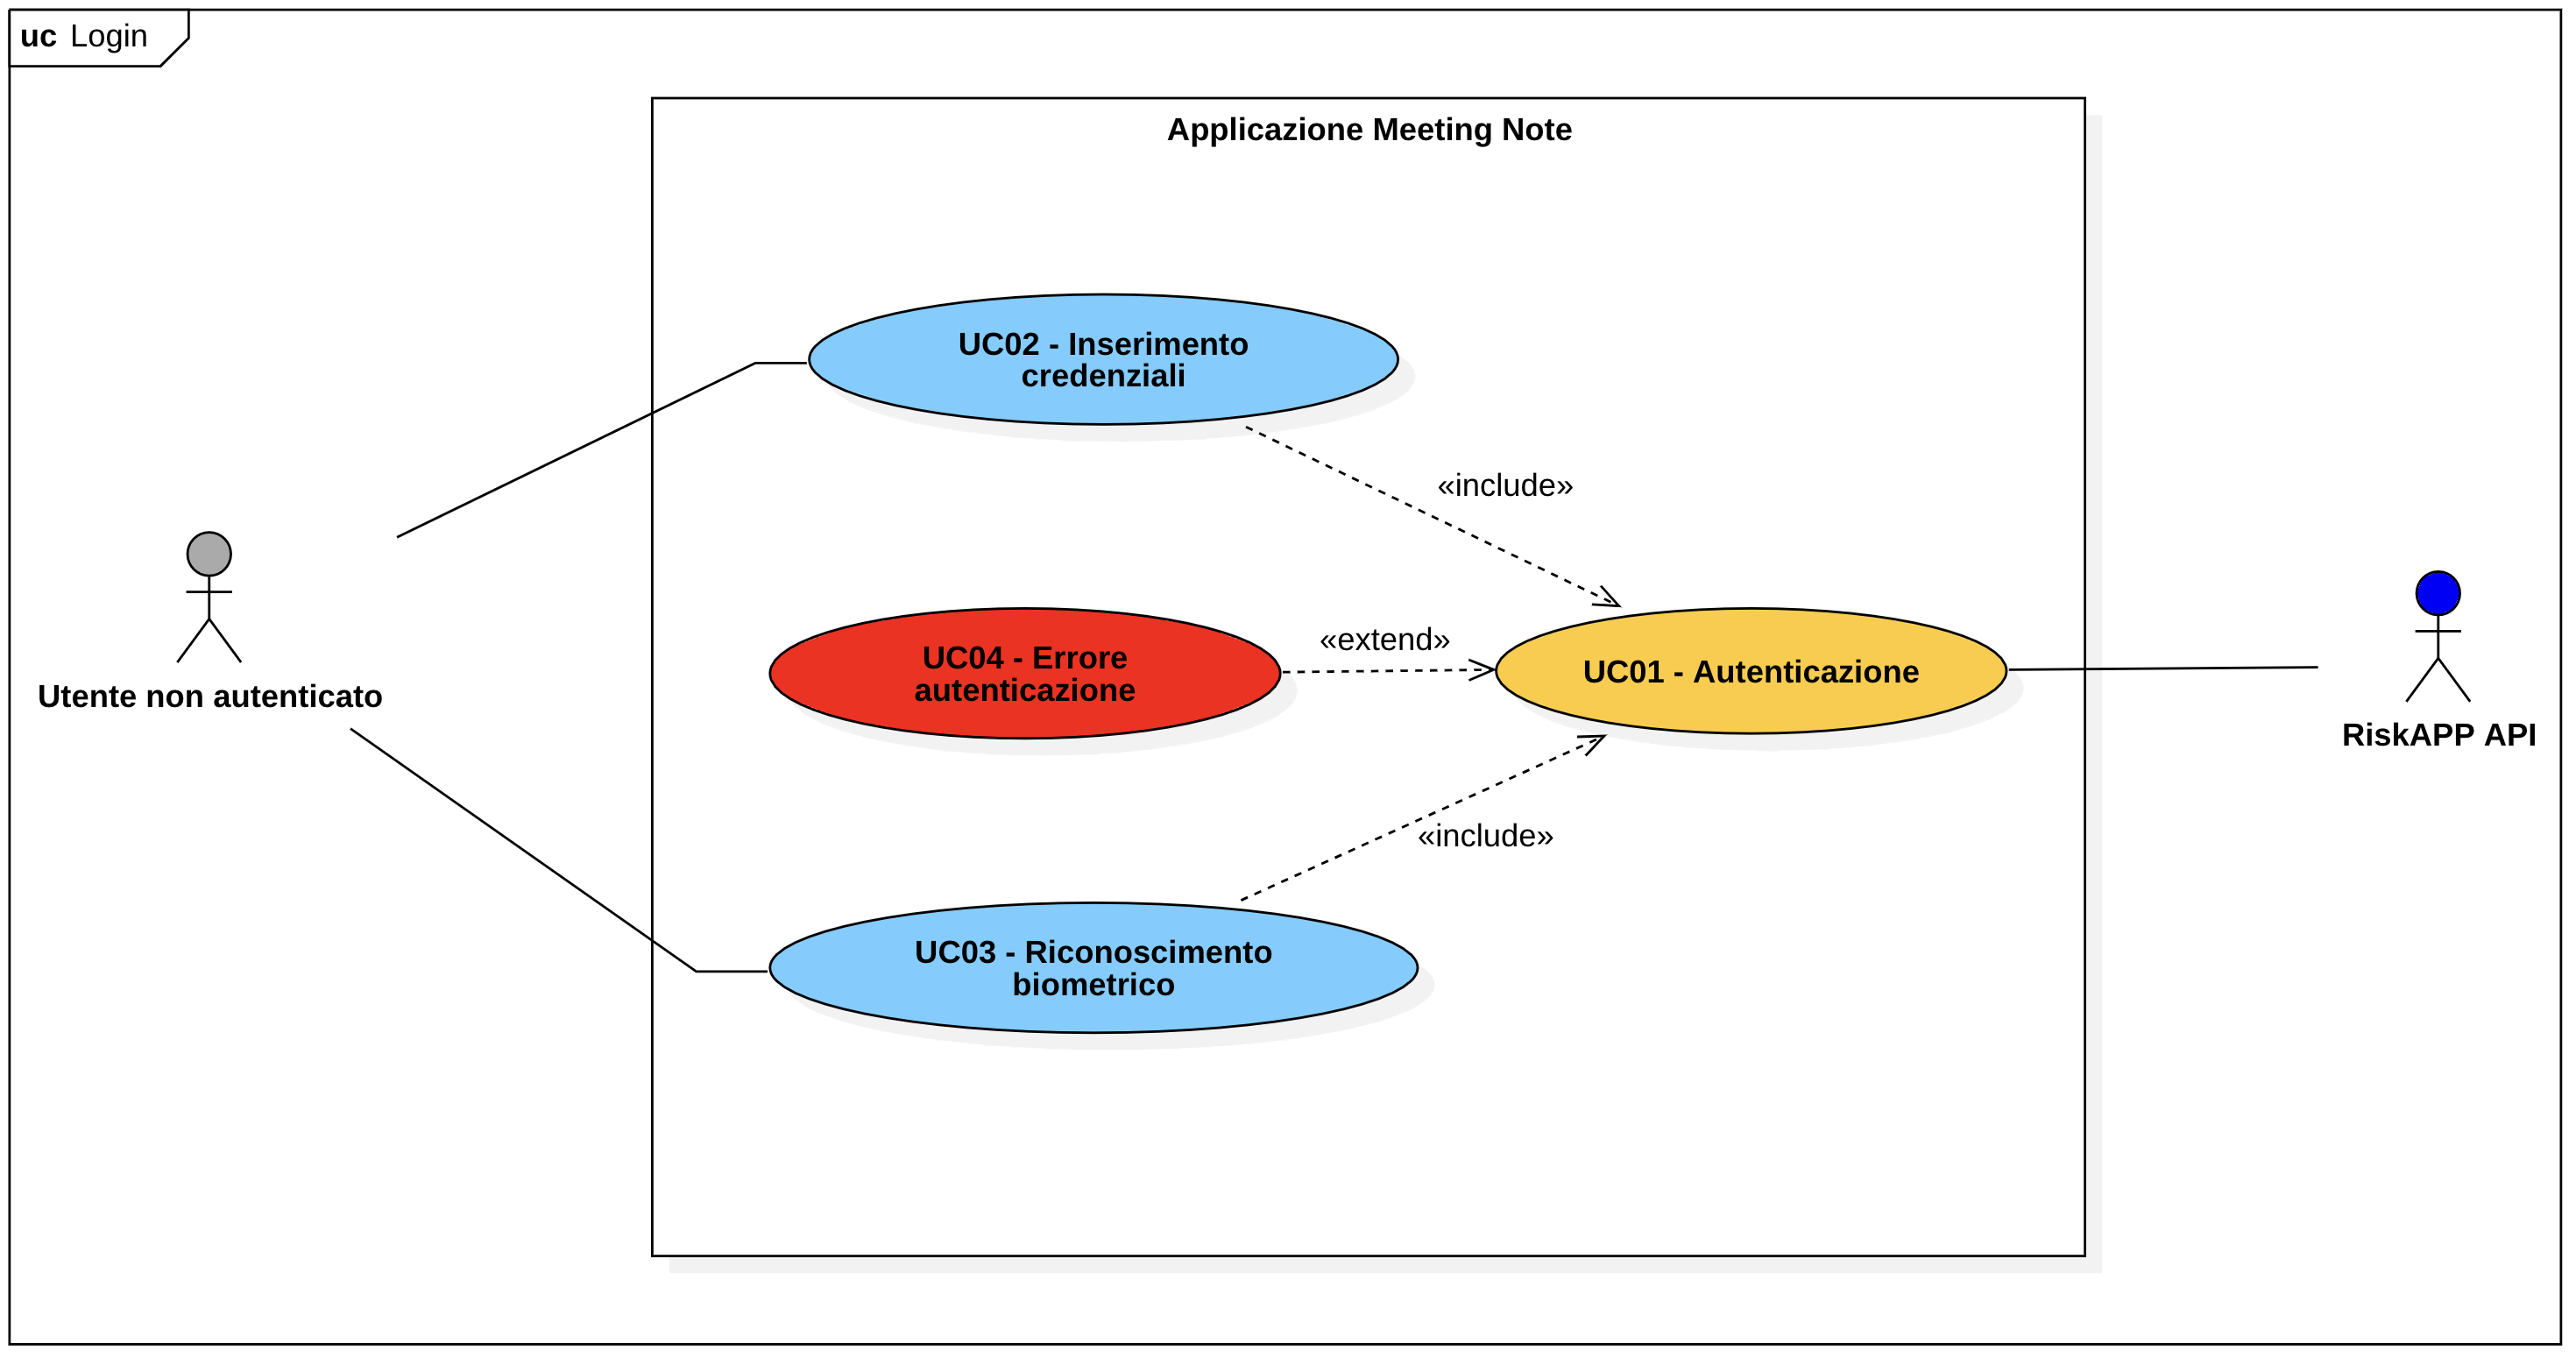
\includegraphics[width=1.0\columnwidth]{usecase/1-uc} 
    \caption{Use Case - Login}
    \label{fig:uc-login}
\end{figure}

\begin{usecase}{01}{Autenticazione}
    \usecasemainactors{Utente non autenticato}
    \usecasesecondaryactors{\emph{RiskAPP API}}
    \usecasepre{L'utente non è ancora autenticato nel sistema}
    \usecasedesc{L'utente effettua l'autenticazione al sistema, scegliendo se farlo, inserendo manualmente le credenziali, oppure tramite \gls{riconoscimentobiometrico}\glsoccur.}
    \usecasepost{L'utente è autenticato nel sistema}
    \usecasealt{Se l'autenticazione fallisce, si verifica \hyperref[UC04]{UC04}}
    \usecaseimg{\ref{fig:uc-login}}
    \label{UC01}
\end{usecase}

\begin{usecase}{02}{Inserimento credenziali}
    \usecasemainactors{Utente non autenticato}
    \usecasepre{L'utente non è ancora autenticato nel sistema}
    \usecasedesc{L'utente inserisce manualmente le proprie credenziali per effettuare l'autenticazione al sistema.}
    \usecasepost{L'utente è autenticato nel sistema}
    \usecaseimg{\ref{fig:uc-login}}
    \label{UC02}
\end{usecase}

\begin{usecase}{03}{Riconoscimento biometrico}
    \usecasemainactors{Utente non autenticato}
    \usecasepre{L'utente non è ancora autenticato nel sistema}
    \usecasedesc{L'utente utilizza il \gls{riconoscimentobiometrico}\glsoccur per effettuare l'autenticazione al sistema.}
    \usecasepost{L'utente è autenticato nel sistema}
    \usecaseimg{\ref{fig:uc-login}}
    \label{UC03}
\end{usecase}

\begin{usecase}{04}{Errore autenticazione}
    \usecasemainactors{Utente non autenticato}
    \usecasesecondaryactors{\emph{RiskAPP API}}
    \usecasepre{L'utente non è ancora autenticato nel sistema}
    \usecasedesc{L'autenticazione fallisce e l'utente viene informato dell'errore; le motivazioni possono essere le seguenti:
        \begin{itemize}
            \item le credenziali inserite non sono corrette;
            \item il sistema non è raggiungibile;
            \item il \gls{riconoscimentobiometrico}\glsoccur è fallito;
            \item connessione ad internet assente.
        \end{itemize}}
    \usecasepost{L'utente non è autenticato nel sistema}
    \usecaseimg{\ref{fig:uc-login}}
    \label{UC04}
\end{usecase}

\begin{figure}[!h] 
    \centering 
    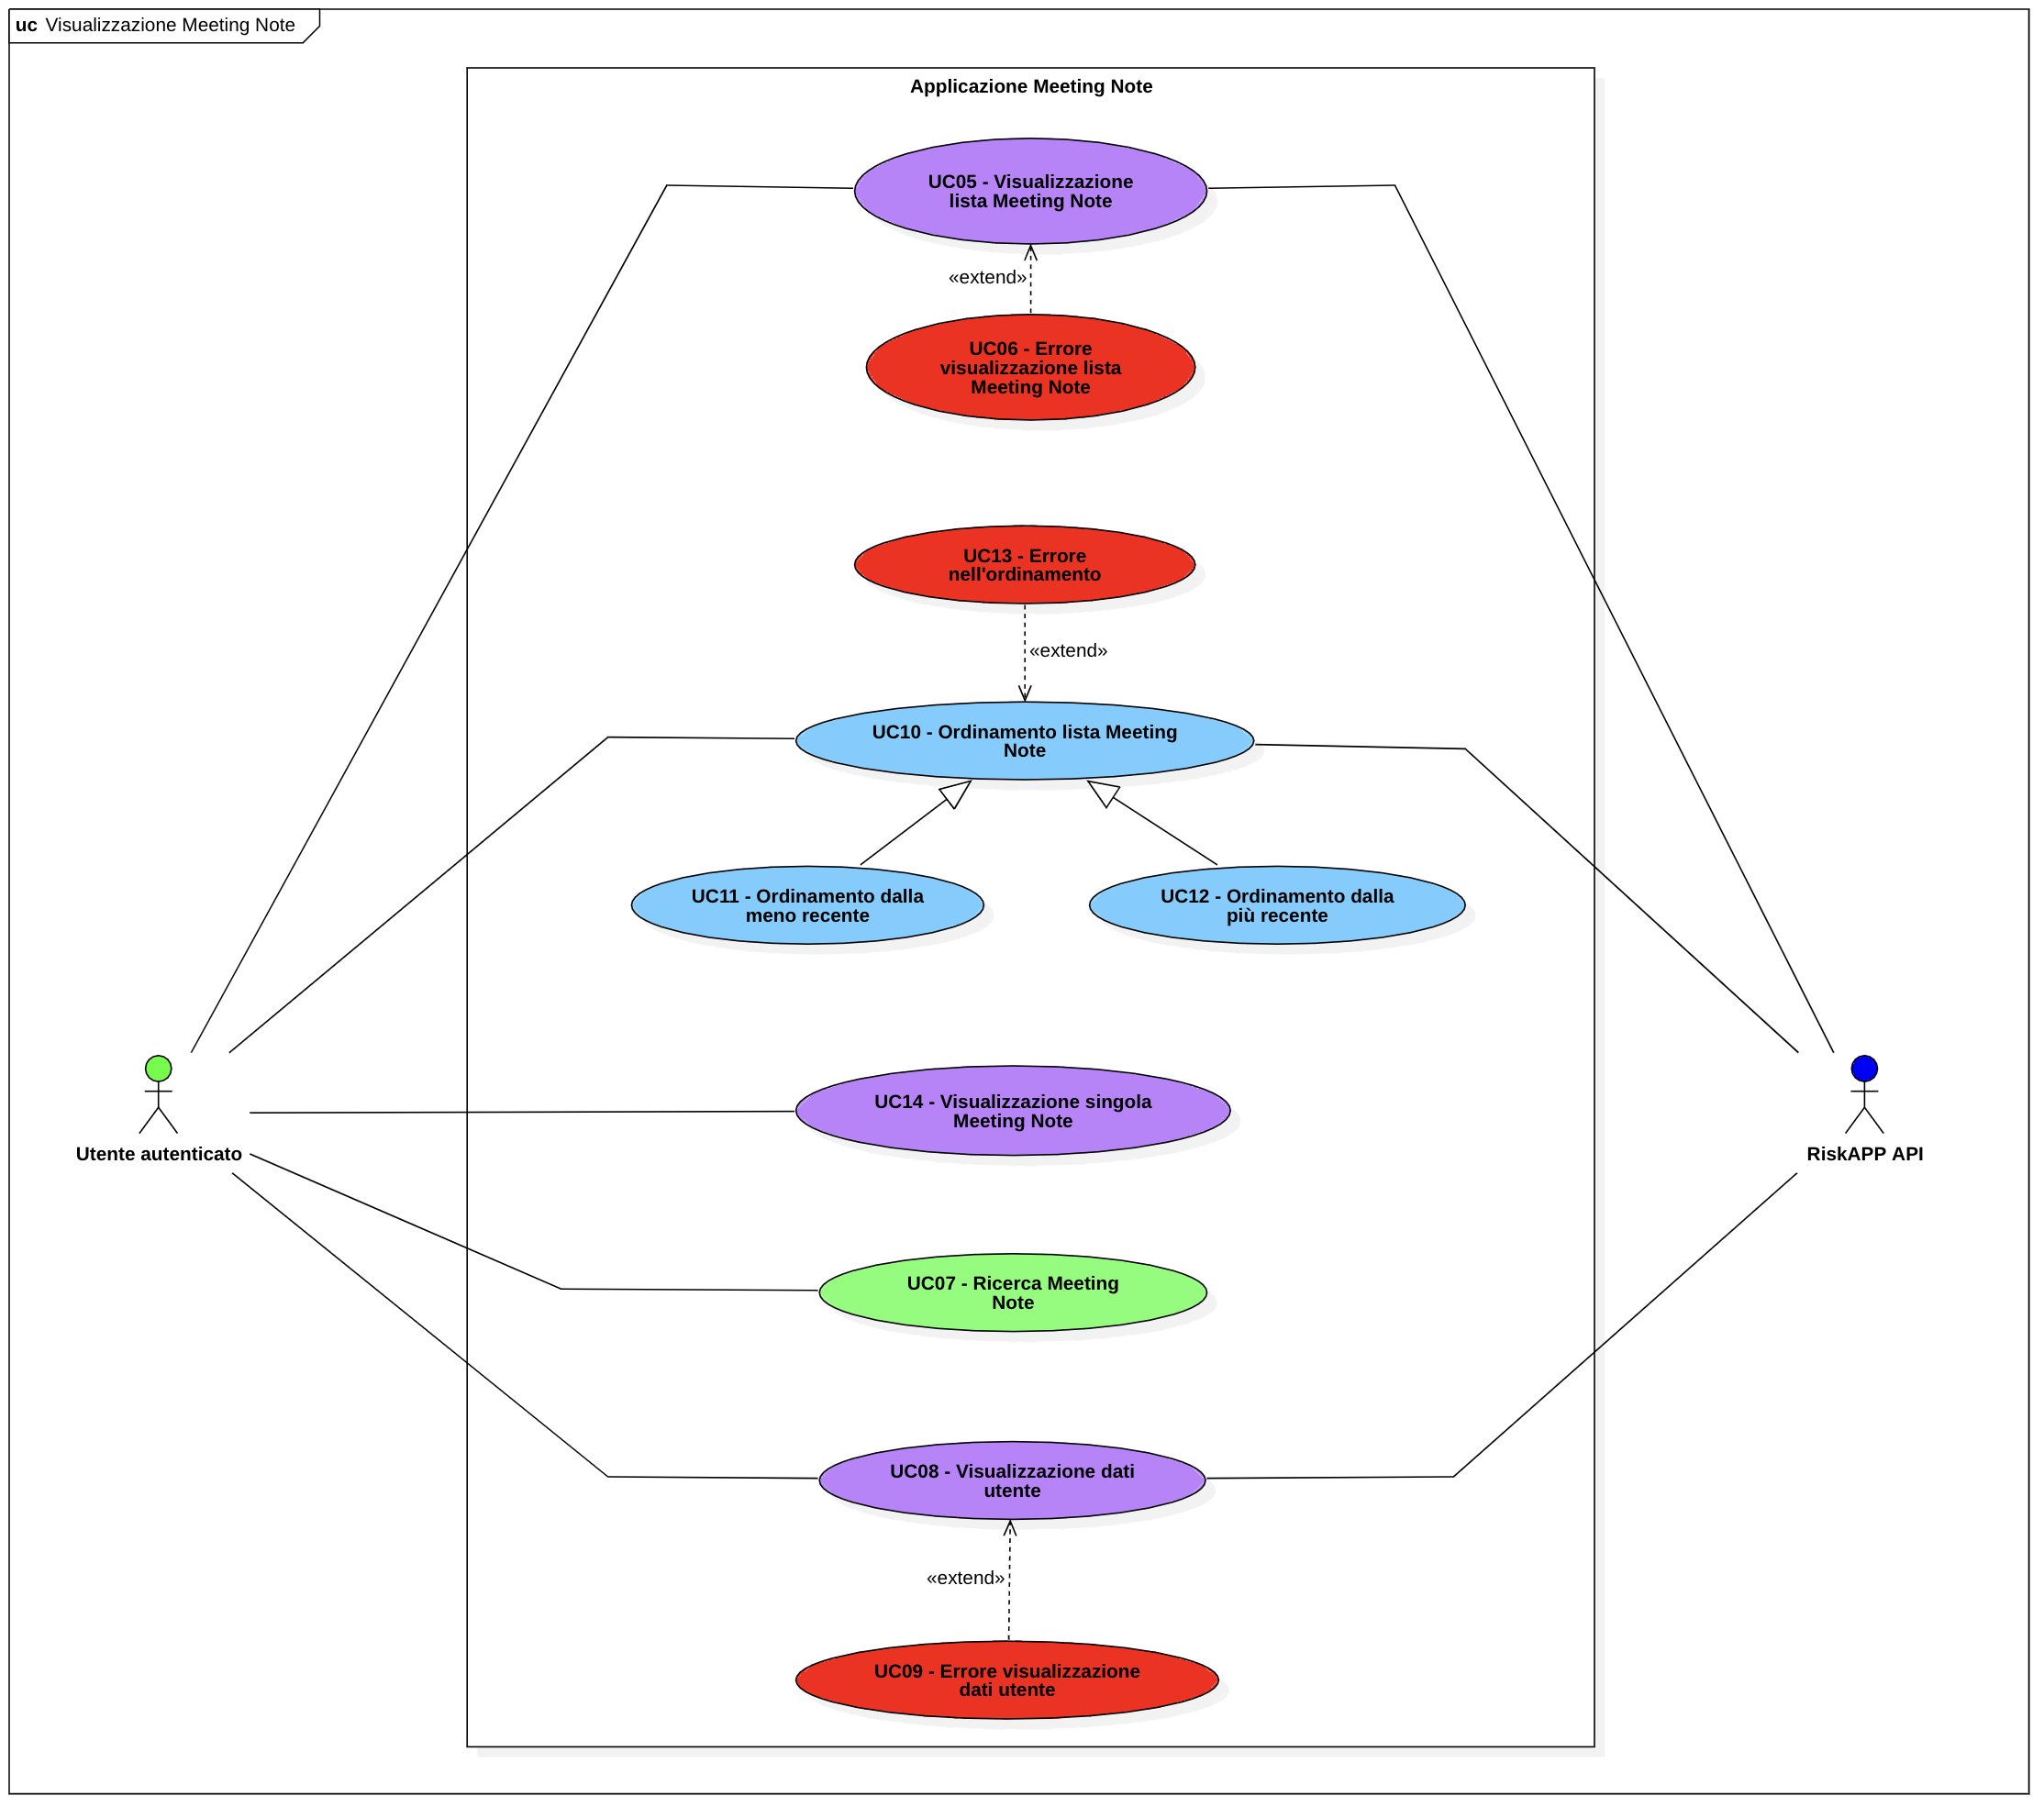
\includegraphics[width=1.0\columnwidth]{usecase/2-uc} 
    \caption{Use Case - Visualizzazione Meeting Note}
    \label{fig:uc-meetingnote}
\end{figure}

\begin{usecase}{05}{Visualizzazione lista Meeting Note}
    \usecasemainactors{Utente autenticato}
    \usecasesecondaryactors{\emph{RiskAPP API}}
    \usecasepre{L'utente è autenticato nel sistema}
    \usecasedesc{L'utente vuole visualizzare la lista di tutte le \gls{meetingnote}\glsoccur associate.}
    \usecasepost{È visualizzabile la lista delle \gls{meetingnote}\glsoccur}
    \usecasealt{Se la visualizzazione fallisce, si verifica \hyperref[UC06]{UC06}}
    \usecaseimg{\ref{fig:uc-meetingnote}}
    \label{UC05}
\end{usecase}

\begin{figure}[!h] 
    \centering 
    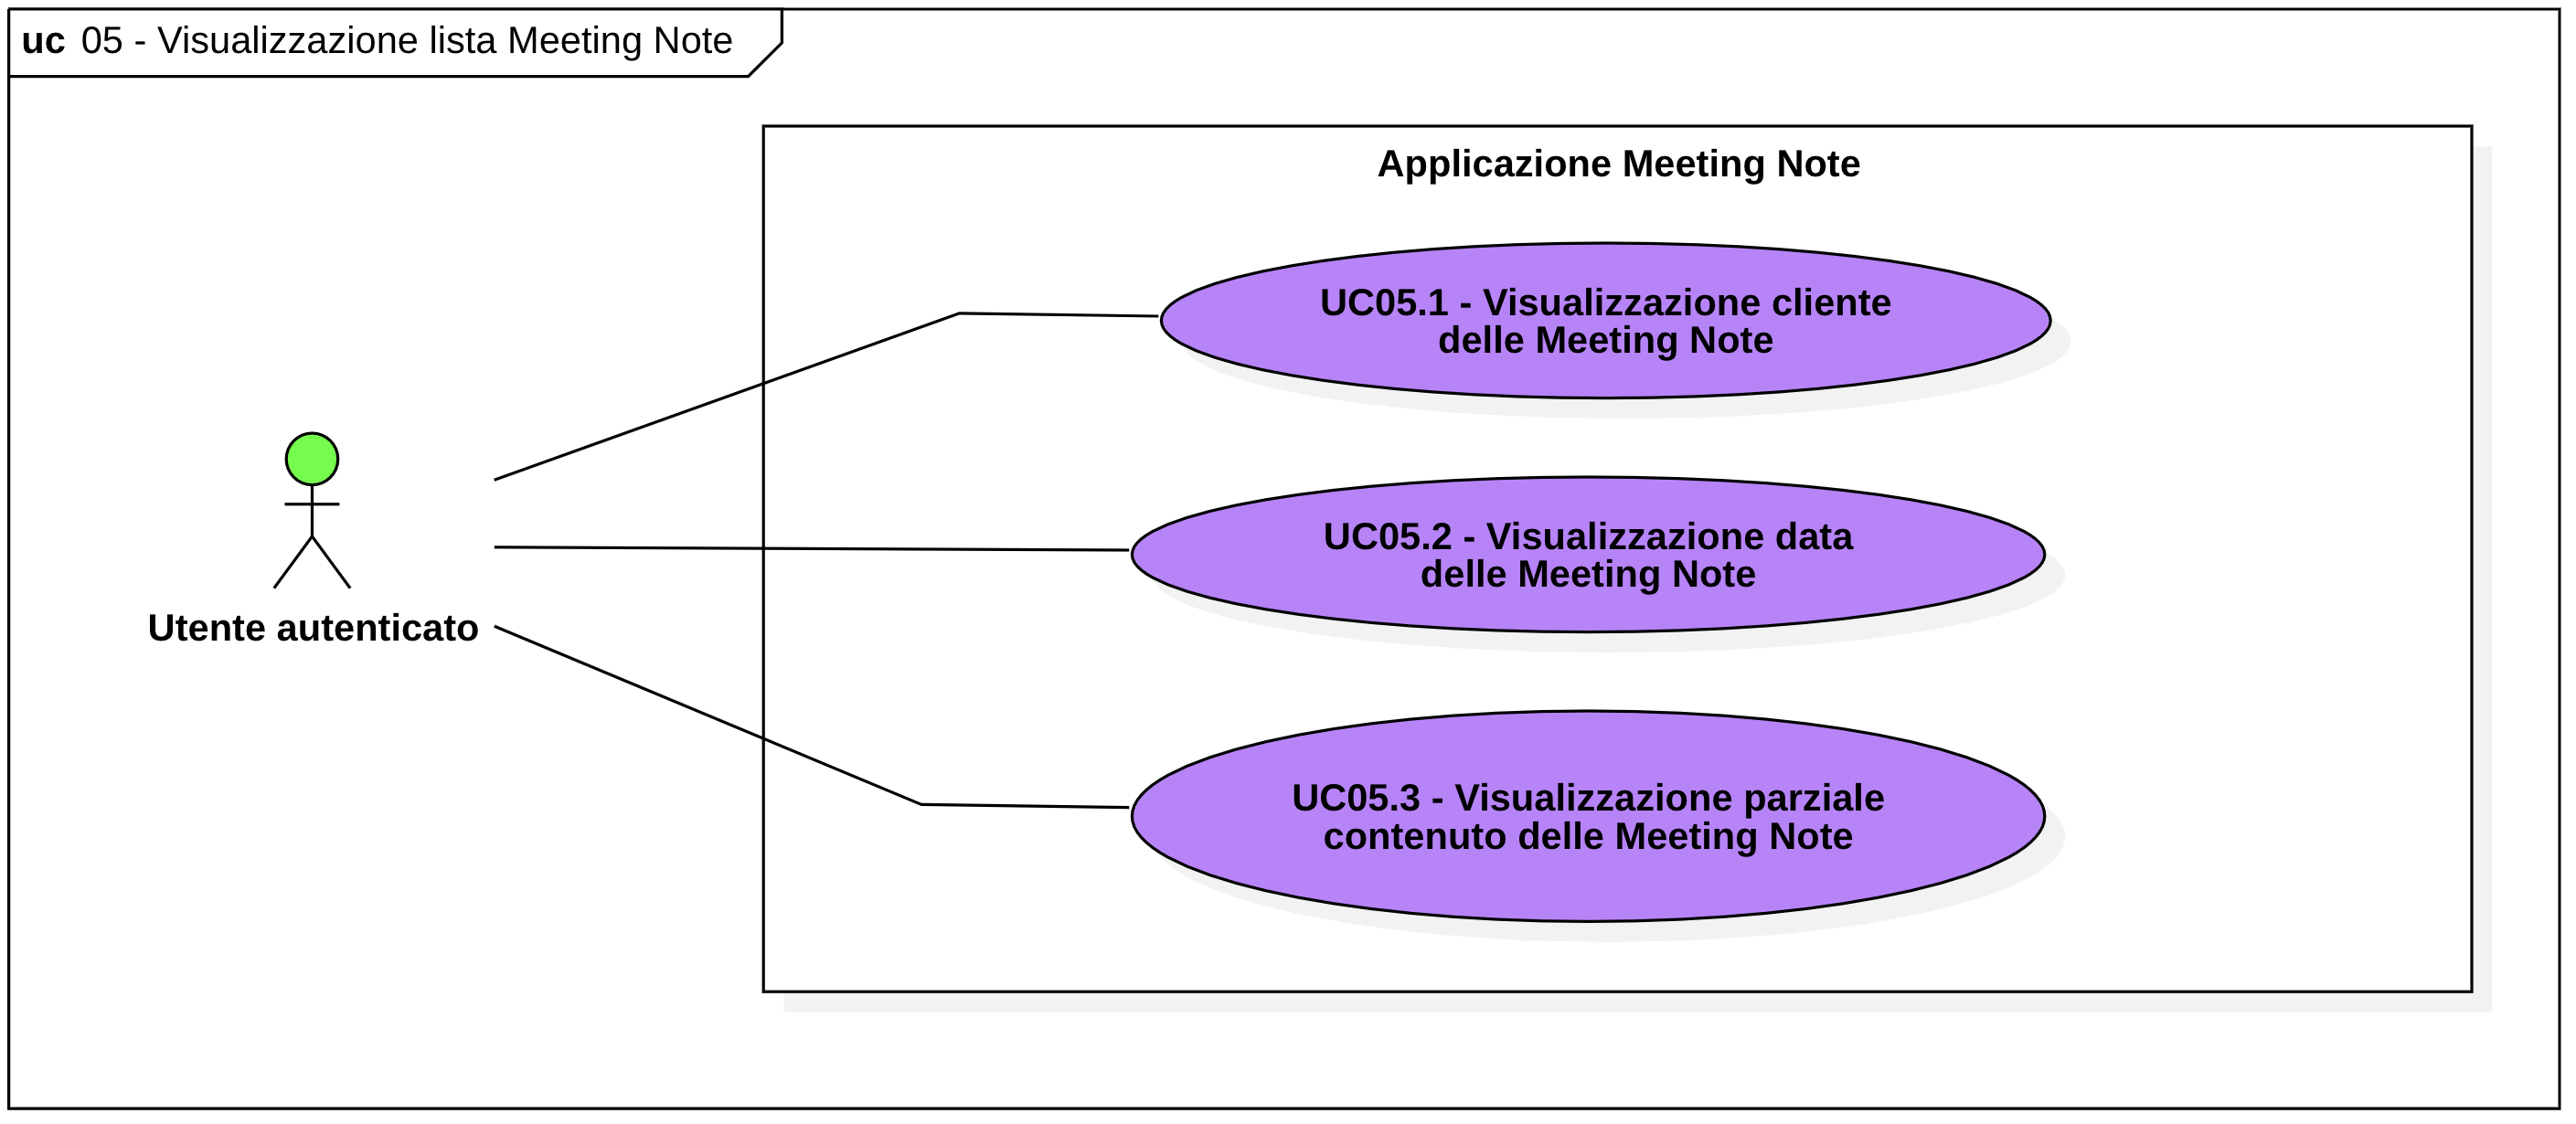
\includegraphics[width=1.0\columnwidth]{usecase/3-uc} 
    \caption{Use Case - Visualizzazione lista Meeting Note}
    \label{fig:uc-meetingnote-list-details}
\end{figure}

\begin{usecase}{05.1}{Visualizzazione cliente delle Meeting Note}
    \usecasemainactors{Utente autenticato}
    \usecasepre{L'utente visualizza la lista delle \gls{meetingnote}\glsoccur}
    \usecasedesc{L'utente vuole visualizzare gli identificativi dei \glspl{cliente}\glsoccur associati alle \gls{meetingnote}\glsoccur.}
    \usecasepost{Sono visualizzabili i \glspl{cliente}\glsoccur associati alle \gls{meetingnote}\glsoccur}
    \usecaseimg{\ref{fig:uc-meetingnote-list-details}}
    \label{UC05.1}
\end{usecase}

\begin{usecase}{05.2}{Visualizzazione data della Meeting Note}
    \usecasemainactors{Utente autenticato}
    \usecasepre{L'utente visualizza la lista delle \gls{meetingnote}\glsoccur}
    \usecasedesc{L'utente vuole visualizzare le date degli incontri associati alle \gls{meetingnote}\glsoccur.}
    \usecasepost{Sono visualizzabili le date degli incontri associati alle \gls{meetingnote}\glsoccur}
    \usecaseimg{\ref{fig:uc-meetingnote-list-details}}
    \label{UC05.2}
\end{usecase}

\begin{usecase}{05.3}{Visualizzazione parziale contenuto delle Meeting Note}
    \usecasemainactors{Utente autenticato}
    \usecasepre{L'utente visualizza la lista delle \gls{meetingnote}\glsoccur}
    \usecasedesc{L'utente vuole visualizzare parzialmente i contenuti delle \gls{meetingnote}\glsoccur.}
    \usecasepost{Sono visualizzabili parzialmente i contenuti delle \gls{meetingnote}\glsoccur}
    \usecaseimg{\ref{fig:uc-meetingnote-list-details}}
    \label{UC05.3}
\end{usecase}

\begin{usecase}{06}{Errore visualizzazione lista Meeting Note}
    \usecasemainactors{Utente autenticato}
    \usecasesecondaryactors{\emph{RiskAPP API}}
    \usecasepre{L'utente è autenticato nel sistema}
    \usecasedesc{La visualizzazione della lista delle \gls{meetingnote}\glsoccur fallisce e l'utente viene informato dell'errore; le motivazioni possono essere le seguenti:
        \begin{itemize}
            \item la lista è vuota;
            \item il sistema non è raggiungibile;
            \item token di autenticazione scaduto;
            \item connessione ad internet assente.
        \end{itemize}}
    \usecasepost{Non è visualizzabile la lista delle \gls{meetingnote}\glsoccur}
    \usecaseimg{\ref{fig:uc-meetingnote}}
    \label{UC06}
\end{usecase}

\begin{usecase}{07}{Ricerca Meeting Note}
    \usecasemainactors{Utente autenticato}
    \usecasepre{L'utente visualizza la lista delle \gls{meetingnote}\glsoccur a lui associate}
    \usecasedesc{L'utente effettua una ricerca all'interno della lista delle \gls{meetingnote}\glsoccur.}
    \usecasepost{Lista delle \gls{meetingnote}\glsoccur è filtrata}
    \usecaseimg{\ref{fig:uc-meetingnote}}
    \label{UC07}
\end{usecase}

\newpage

\begin{figure}[!h] 
    \centering 
    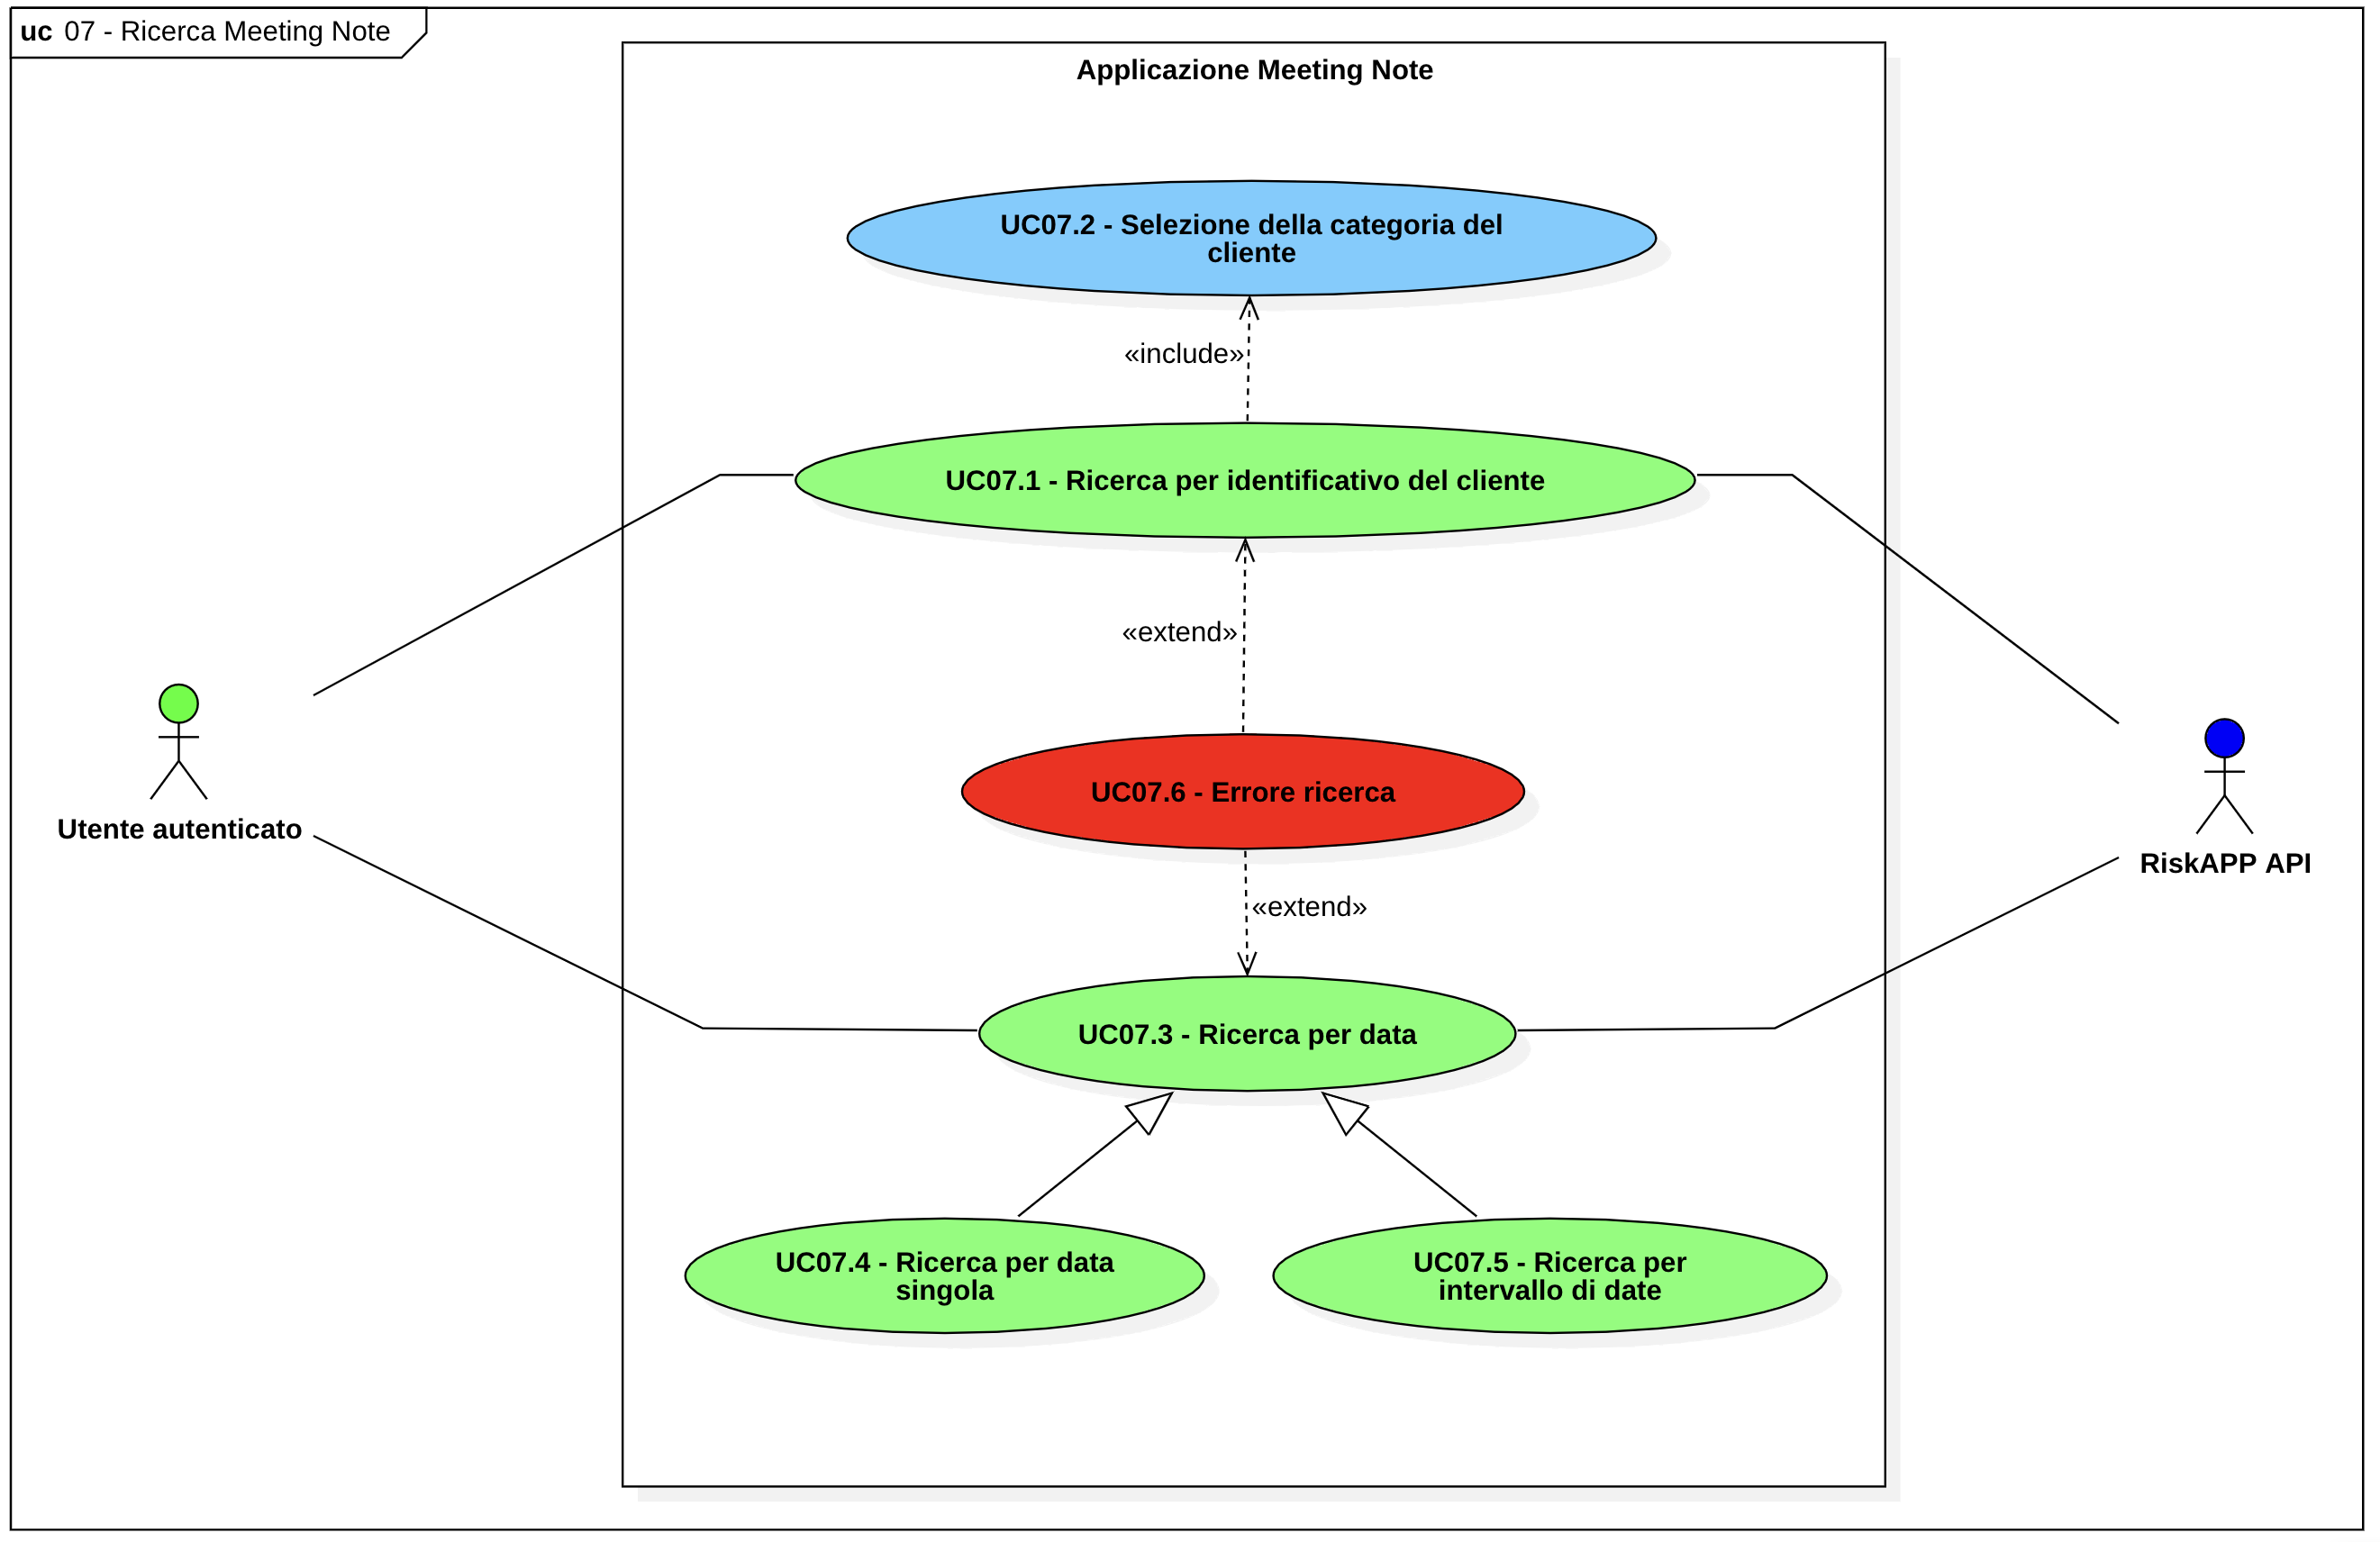
\includegraphics[width=1.0\columnwidth]{usecase/4-uc} 
    \caption{Use Case - Ricerca Meeting Note}
    \label{fig:uc-meetingnote-search}
\end{figure}

\begin{usecase}{07.1}{Ricerca per identificativo del cliente}
    \usecasemainactors{Utente autenticato}
    \usecasesecondaryactors{\emph{RiskAPP API}}
    \usecasepre{L'utente ha selezionato la categoria del \gls{cliente}\glsoccur}
    \usecasedesc{L'utente effettua una ricerca per identificativo del \gls{cliente}\glsoccur all'interno della lista delle \gls{meetingnote}\glsoccur.}
    \usecasepost{Lista delle \gls{meetingnote}\glsoccur è filtrata per identificativo del \gls{cliente}\glsoccur}
    \usecasealt{Se la ricerca fallisce, si verifica \hyperref[UC07.6]{UC07.6}}
    \usecaseimg{\ref{fig:uc-meetingnote-search}}
    \label{UC07.1}
\end{usecase}

\begin{usecase}{07.2}{Selezione della categoria del cliente}
    \usecasemainactors{Utente autenticato}
    \usecasepre{L'utente visualizza la lista delle \gls{meetingnote}\glsoccur a lui associate}
    \usecasedesc{L'utente seleziona la categoria del \gls{cliente}\glsoccur per effettuare la ricerca per identificativo all'interno della lista delle \gls{meetingnote}\glsoccur.}
    \usecasepost{La categoria del \gls{cliente}\glsoccur è selezionata}
    \usecaseimg{\ref{fig:uc-meetingnote-search}}
    \label{UC07.2}
\end{usecase}

\begin{usecase}{07.3}{Ricerca per data}
    \usecasemainactors{Utente autenticato}
    \usecasesecondaryactors{\emph{RiskAPP API}}
    \usecasepre{L'utente visualizza la lista delle \gls{meetingnote}\glsoccur a lui associate}
    \usecasedesc{L'utente effettua una ricerca per data all'interno della lista delle \gls{meetingnote}\glsoccur.}
    \usecasepost{Lista delle \gls{meetingnote}\glsoccur è filtrata per data}
    \usecasealt{Se la ricerca fallisce, si verifica \hyperref[UC07.6]{UC07.6}}
    \usecaseimg{\ref{fig:uc-meetingnote-search}}
    \label{UC07.3}
\end{usecase}

\begin{usecase}{07.4}{Ricerca per data singola}
    \usecasemainactors{Utente autenticato}
    \usecasepre{L'utente visualizza la lista delle \gls{meetingnote}\glsoccur a lui associate}
    \usecasedesc{L'utente effettua una ricerca per data singola all'interno della lista delle \gls{meetingnote}\glsoccur.}
    \usecasepost{Lista delle \gls{meetingnote}\glsoccur è filtrata per data singola}
    \usecaseimg{\ref{fig:uc-meetingnote-search}}
    \label{UC07.4}
\end{usecase}

\begin{usecase}{07.5}{Ricerca per intervallo di date}
    \usecasemainactors{Utente autenticato}
    \usecasepre{L'utente visualizza la lista delle \gls{meetingnote}\glsoccur a lui associate}
    \usecasedesc{L'utente effettua una ricerca per intervallo di date all'interno della lista delle \gls{meetingnote}\glsoccur.}
    \usecasepost{Lista delle \gls{meetingnote}\glsoccur è filtrata per intervallo di date}
    \usecaseimg{\ref{fig:uc-meetingnote-search}}
    \label{UC07.5}
\end{usecase}

\begin{usecase}{07.6}{Errore ricerca}
    \usecasemainactors{Utente autenticato}
    \usecasesecondaryactors{\emph{RiskAPP API}}
    \usecasepre{L'utente ha effettuato una ricerca all'interno della lista delle \gls{meetingnote}\glsoccur}
    \usecasedesc{La ricerca fallisce e l'utente viene informato dell'errore; le motivazioni possono essere le seguenti:
        \begin{itemize}
            \item la lista risultante è vuota;
            \item il sistema non è raggiungibile;
            \item token di autenticazione scaduto;
            \item connessione ad internet assente.
        \end{itemize}}
    \usecasepost{Lista delle \gls{meetingnote}\glsoccur non è filtrata}
    \usecaseimg{\ref{fig:uc-meetingnote-search}}
    \label{UC07.6}
\end{usecase}

\begin{usecase}{08}{Visualizzazione dati utente}
    \usecasemainactors{Utente autenticato}
    \usecasesecondaryactors{\emph{RiskAPP API}}
    \usecasepre{L'utente è autenticato nel sistema}
    \usecasedesc{L'utente vuole visualizzare i propri dati personali.}
    \usecasepost{Sono visualizzabili i dati personali dell'utente}
    \usecasealt{Se la visualizzazione fallisce, si verifica \hyperref[UC09]{UC09}} 
    \usecaseimg{\ref{fig:uc-meetingnote}}
    \label{UC08}
\end{usecase}

\begin{figure}[!h] 
    \centering 
    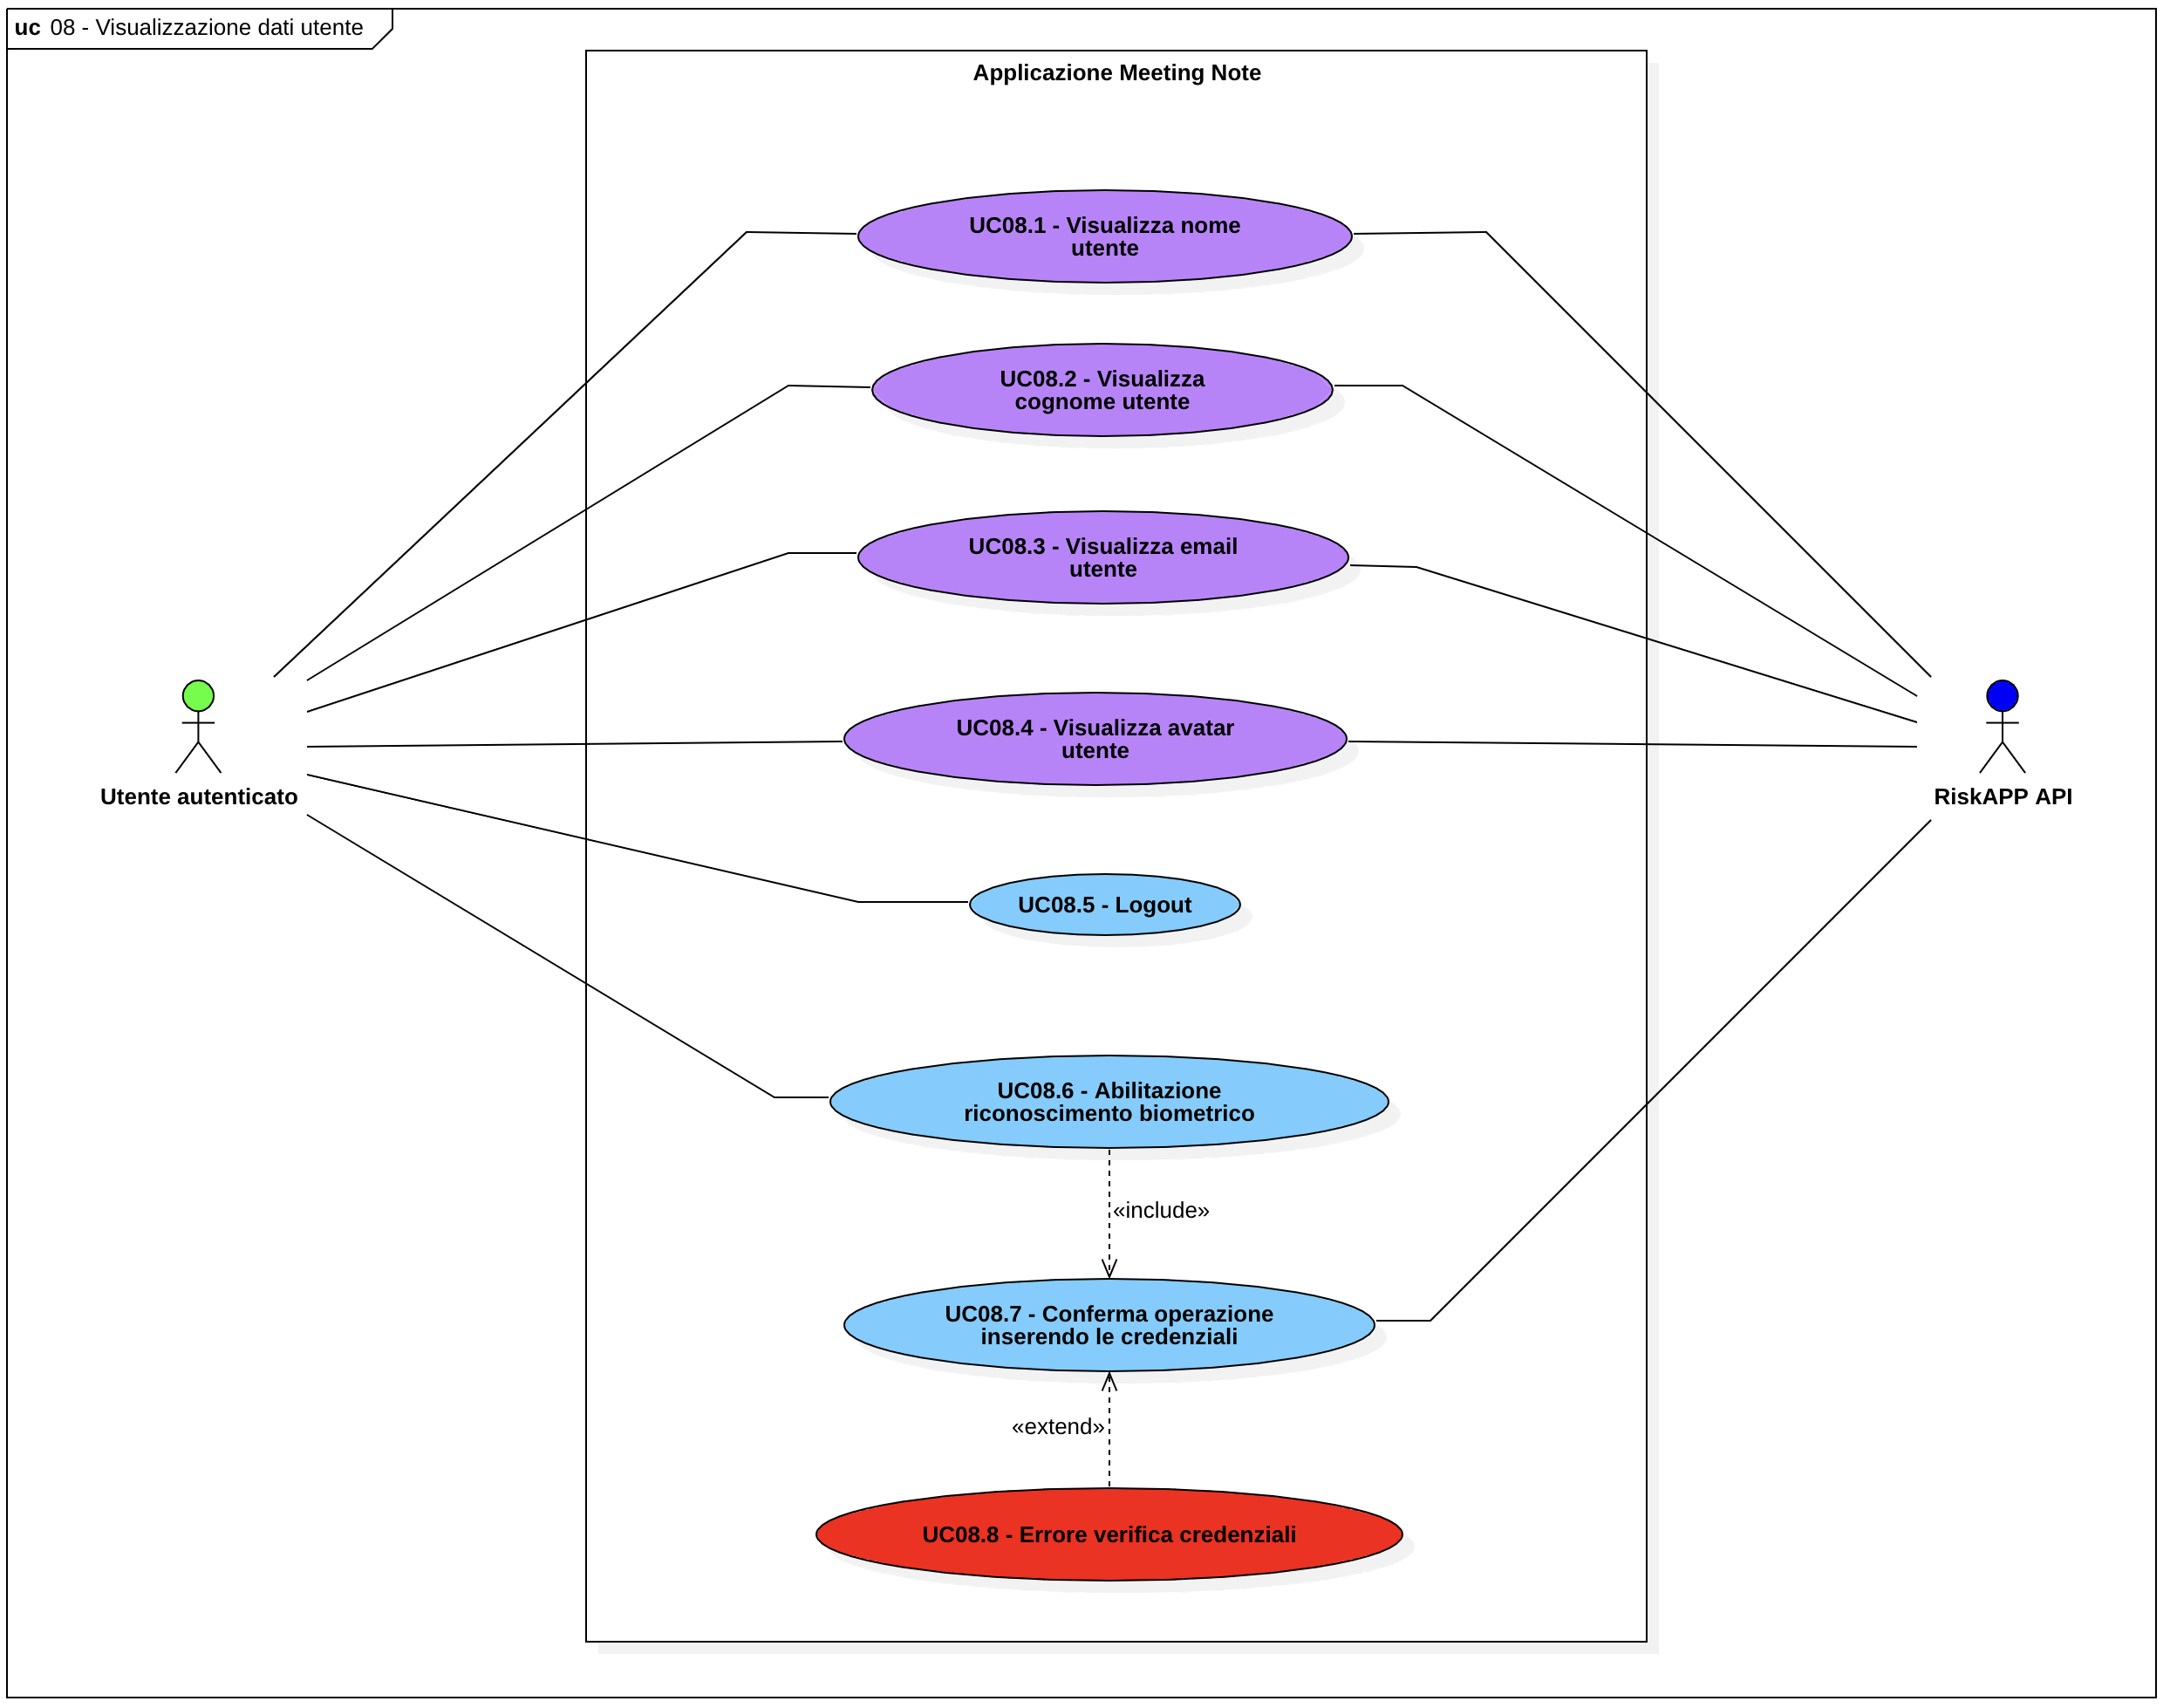
\includegraphics[width=1.0\columnwidth]{usecase/5-uc} 
    \caption{Use Case - Visualizzazione dati utente}
    \label{fig:uc-user}
\end{figure}

\begin{usecase}{08.1}{Visualizzazione nome utente}
    \usecasemainactors{Utente autenticato}
    \usecasesecondaryactors{\emph{RiskAPP API}}
    \usecasepre{L'utente visualizza i propri dati personali}
    \usecasedesc{L'utente vuole visualizzare il proprio nome.}
    \usecasepost{È visualizzabile il nome dell'utente}
    \usecaseimg{\ref{fig:uc-user}}
    \label{UC08.1}
\end{usecase}

\begin{usecase}{08.2}{Visualizzazione cognome utente}
    \usecasemainactors{Utente autenticato}
    \usecasesecondaryactors{\emph{RiskAPP API}}
    \usecasepre{L'utente visualizza i propri dati personali}
    \usecasedesc{L'utente vuole visualizzare il proprio cognome.}
    \usecasepost{È visualizzabile il cognome dell'utente}
    \usecaseimg{\ref{fig:uc-user}}
    \label{UC08.2}
\end{usecase}

\begin{usecase}{08.3}{Visualizzazione email utente}
    \usecasemainactors{Utente autenticato}
    \usecasesecondaryactors{\emph{RiskAPP API}}
    \usecasepre{L'utente visualizza i propri dati personali}
    \usecasedesc{L'utente vuole visualizzare la propria email.}
    \usecasepost{È visualizzabile la email dell'utente}
    \usecaseimg{\ref{fig:uc-user}}
    \label{UC08.3}
\end{usecase}

\begin{usecase}{08.4}{Visualizzazione avatar utente}
    \usecasemainactors{Utente autenticato}
    \usecasesecondaryactors{\emph{RiskAPP API}}
    \usecasepre{L'utente visualizza i propri dati personali}
    \usecasedesc{L'utente vuole visualizzare il proprio avatar.}
    \usecasepost{È visualizzabile l'avatar dell'utente}
    \usecaseimg{\ref{fig:uc-user}}
    \label{UC08.4}
\end{usecase}

\begin{usecase}{08.5}{Logout}
    \usecasemainactors{Utente autenticato}
    \usecasepre{L'utente visualizza i propri dati personali}
    \usecasedesc{L'utente vuole effetuare il logout.}
    \usecasepost{L'utente non è più autenticato al sistema}
    \usecaseimg{\ref{fig:uc-user}}
    \label{UC08.5}
\end{usecase}

\begin{usecase}{08.6}{Abilitazione riconoscimento biometrico}
    \usecasemainactors{Utente autenticato}
    \usecasesecondaryactors{\emph{RiskAPP API}}
    \usecasepre{L'utente visualizza i propri dati personali}
    \usecasedesc{L'utente vuole abilitare il \gls{riconoscimentobiometrico}\glsoccur, deve inserire le proprie credenziali per la conferma.}
    \usecasepost{Riconoscimento biometrico abilitato}
    \usecaseimg{\ref{fig:uc-user}}
    \label{UC08.6}
\end{usecase}

\begin{usecase}{08.7}{Conferma operazione inserendo le credenziali}
    \usecasemainactors{Utente autenticato}
    \usecasesecondaryactors{\emph{RiskAPP API}}
    \usecasepre{L'utente visualizza i propri dati personali}
    \usecasedesc{L'utente inserisce le proprie credenziali per abilitare il \gls{riconoscimentobiometrico}\glsoccur.}
    \usecasepost{Riconoscimento biometrico abilitato}
    \usecasealt{Se la conferma fallisce, si verifica \hyperref[UC08.8]{UC08.8}}
    \usecaseimg{\ref{fig:uc-user}}
    \label{UC08.7}
\end{usecase}

\begin{usecase}{08.8}{Errore verifica credenziali}
    \usecasemainactors{Utente autenticato}
    \usecasesecondaryactors{\emph{RiskAPP API}}
    \usecasepre{L'utente visualizza i propri dati personali}
    \usecasedesc{La verifica delle credenziali fallisce e l'utente viene informato dell'errore; le motivazioni possono essere le seguenti:
        \begin{itemize}
            \item le credenziali inserite non sono corrette;
            \item il sistema non è raggiungibile;
            \item connessione ad internet assente.
        \end{itemize}}
    \usecasepost{Riconoscimento biometrico non abilitato}
    \usecaseimg{\ref{fig:uc-user}}
    \label{UC08.8}
\end{usecase}

\begin{usecase}{09}{Errore visualizzazione dati utente}
    \usecasemainactors{Utente autenticato}
    \usecasesecondaryactors{\emph{RiskAPP API}}
    \usecasepre{L'utente è autenticato nel sistema}
    \usecasedesc{La visualizzazione dei dati utente fallisce e l'utente viene informato dell'errore; le motivazioni possono essere le seguenti:
        \begin{itemize}
            \item il sistema non è raggiungibile;
            \item token di autenticazione scaduto;
            \item connessione ad internet assente.
        \end{itemize}}
    \usecasepost{Non sono visualizzabili i dati personali dell'utente}
    \usecaseimg{\ref{fig:uc-meetingnote}}
    \label{UC09}
\end{usecase}

\begin{usecase}{10}{Ordinamento lista Meeting Note}
    \usecasemainactors{Utente autenticato}
    \usecasesecondaryactors{\emph{RiskAPP API}}
    \usecasepre{L'utente visualizza la lista delle \gls{meetingnote}\glsoccur}
    \usecasedesc{L'utente vuole ordinare la lista delle \gls{meetingnote}\glsoccur.}
    \usecasepost{Lista delle \gls{meetingnote}\glsoccur è ordinata}
    \usecasealt{Se l'ordinamento fallisce, si verifica \hyperref[UC13]{UC13}}
    \usecaseimg{\ref{fig:uc-meetingnote}}
    \label{UC10}
\end{usecase}

\begin{usecase}{11}{Ordinamento dalla meno recente}
    \usecasemainactors{Utente autenticato}
    \usecasesecondaryactors{\emph{RiskAPP API}}
    \usecasepre{L'utente visualizza la lista delle \gls{meetingnote}\glsoccur}
    \usecasedesc{L'utente vuole ordinare la lista delle \gls{meetingnote}\glsoccur dalla meno recente.}
    \usecasepost{Lista delle \gls{meetingnote}\glsoccur è ordinata dalla meno recente}
    \usecasealt{Se l'ordinamento fallisce, si verifica \hyperref[UC13]{UC13}}
    \usecaseimg{\ref{fig:uc-meetingnote}}
    \label{UC11}
\end{usecase}

\begin{usecase}{12}{Ordinamento dalla più recente}
    \usecasemainactors{Utente autenticato}
    \usecasesecondaryactors{\emph{RiskAPP API}}
    \usecasepre{L'utente visualizza la lista delle \gls{meetingnote}\glsoccur}
    \usecasedesc{L'utente vuole ordinare la lista delle \gls{meetingnote}\glsoccur dalla più recente.}
    \usecasepost{Lista delle \gls{meetingnote}\glsoccur è ordinata dalla più recente}
    \usecasealt{Se l'ordinamento fallisce, si verifica \hyperref[UC13]{UC13}}
    \usecaseimg{\ref{fig:uc-meetingnote}}
    \label{UC12}
\end{usecase}

\begin{usecase}{13}{Errore nell'ordinamento}
    \usecasemainactors{Utente autenticato}
    \usecasesecondaryactors{\emph{RiskAPP API}}
    \usecasepre{L'utente vuole ordinare la lista delle \gls{meetingnote}\glsoccur}
    \usecasedesc{L'ordinamento della lista delle \gls{meetingnote}\glsoccur fallisce e l'utente viene informato dell'errore; le motivazioni possono essere le seguenti:
        \begin{itemize}
            \item il sistema non è raggiungibile;
            \item token di autenticazione scaduto;
            \item connessione ad internet assente.
        \end{itemize}}
    \usecasepost{Lista delle \gls{meetingnote}\glsoccur non è ordinata}
    \usecaseimg{\ref{fig:uc-meetingnote}}
    \label{UC13}
\end{usecase}

\begin{usecase}{14}{Visualizzazione singola Meeting Note}
    \usecasemainactors{Utente autenticato}
    \usecasepre{L'utente visualizza la lista delle \gls{meetingnote}\glsoccur}
    \usecasedesc{L'utente vuole visualizzare i dettagli di una singola \gls{meetingnote}\glsoccur.}
    \usecasepost{Sono visualizzabili i dettagli di una singola \gls{meetingnote}\glsoccur}
    \usecaseimg{\ref{fig:uc-meetingnote}}
    \label{UC14}
\end{usecase}

\newpage

\begin{figure}[!h] 
    \centering 
    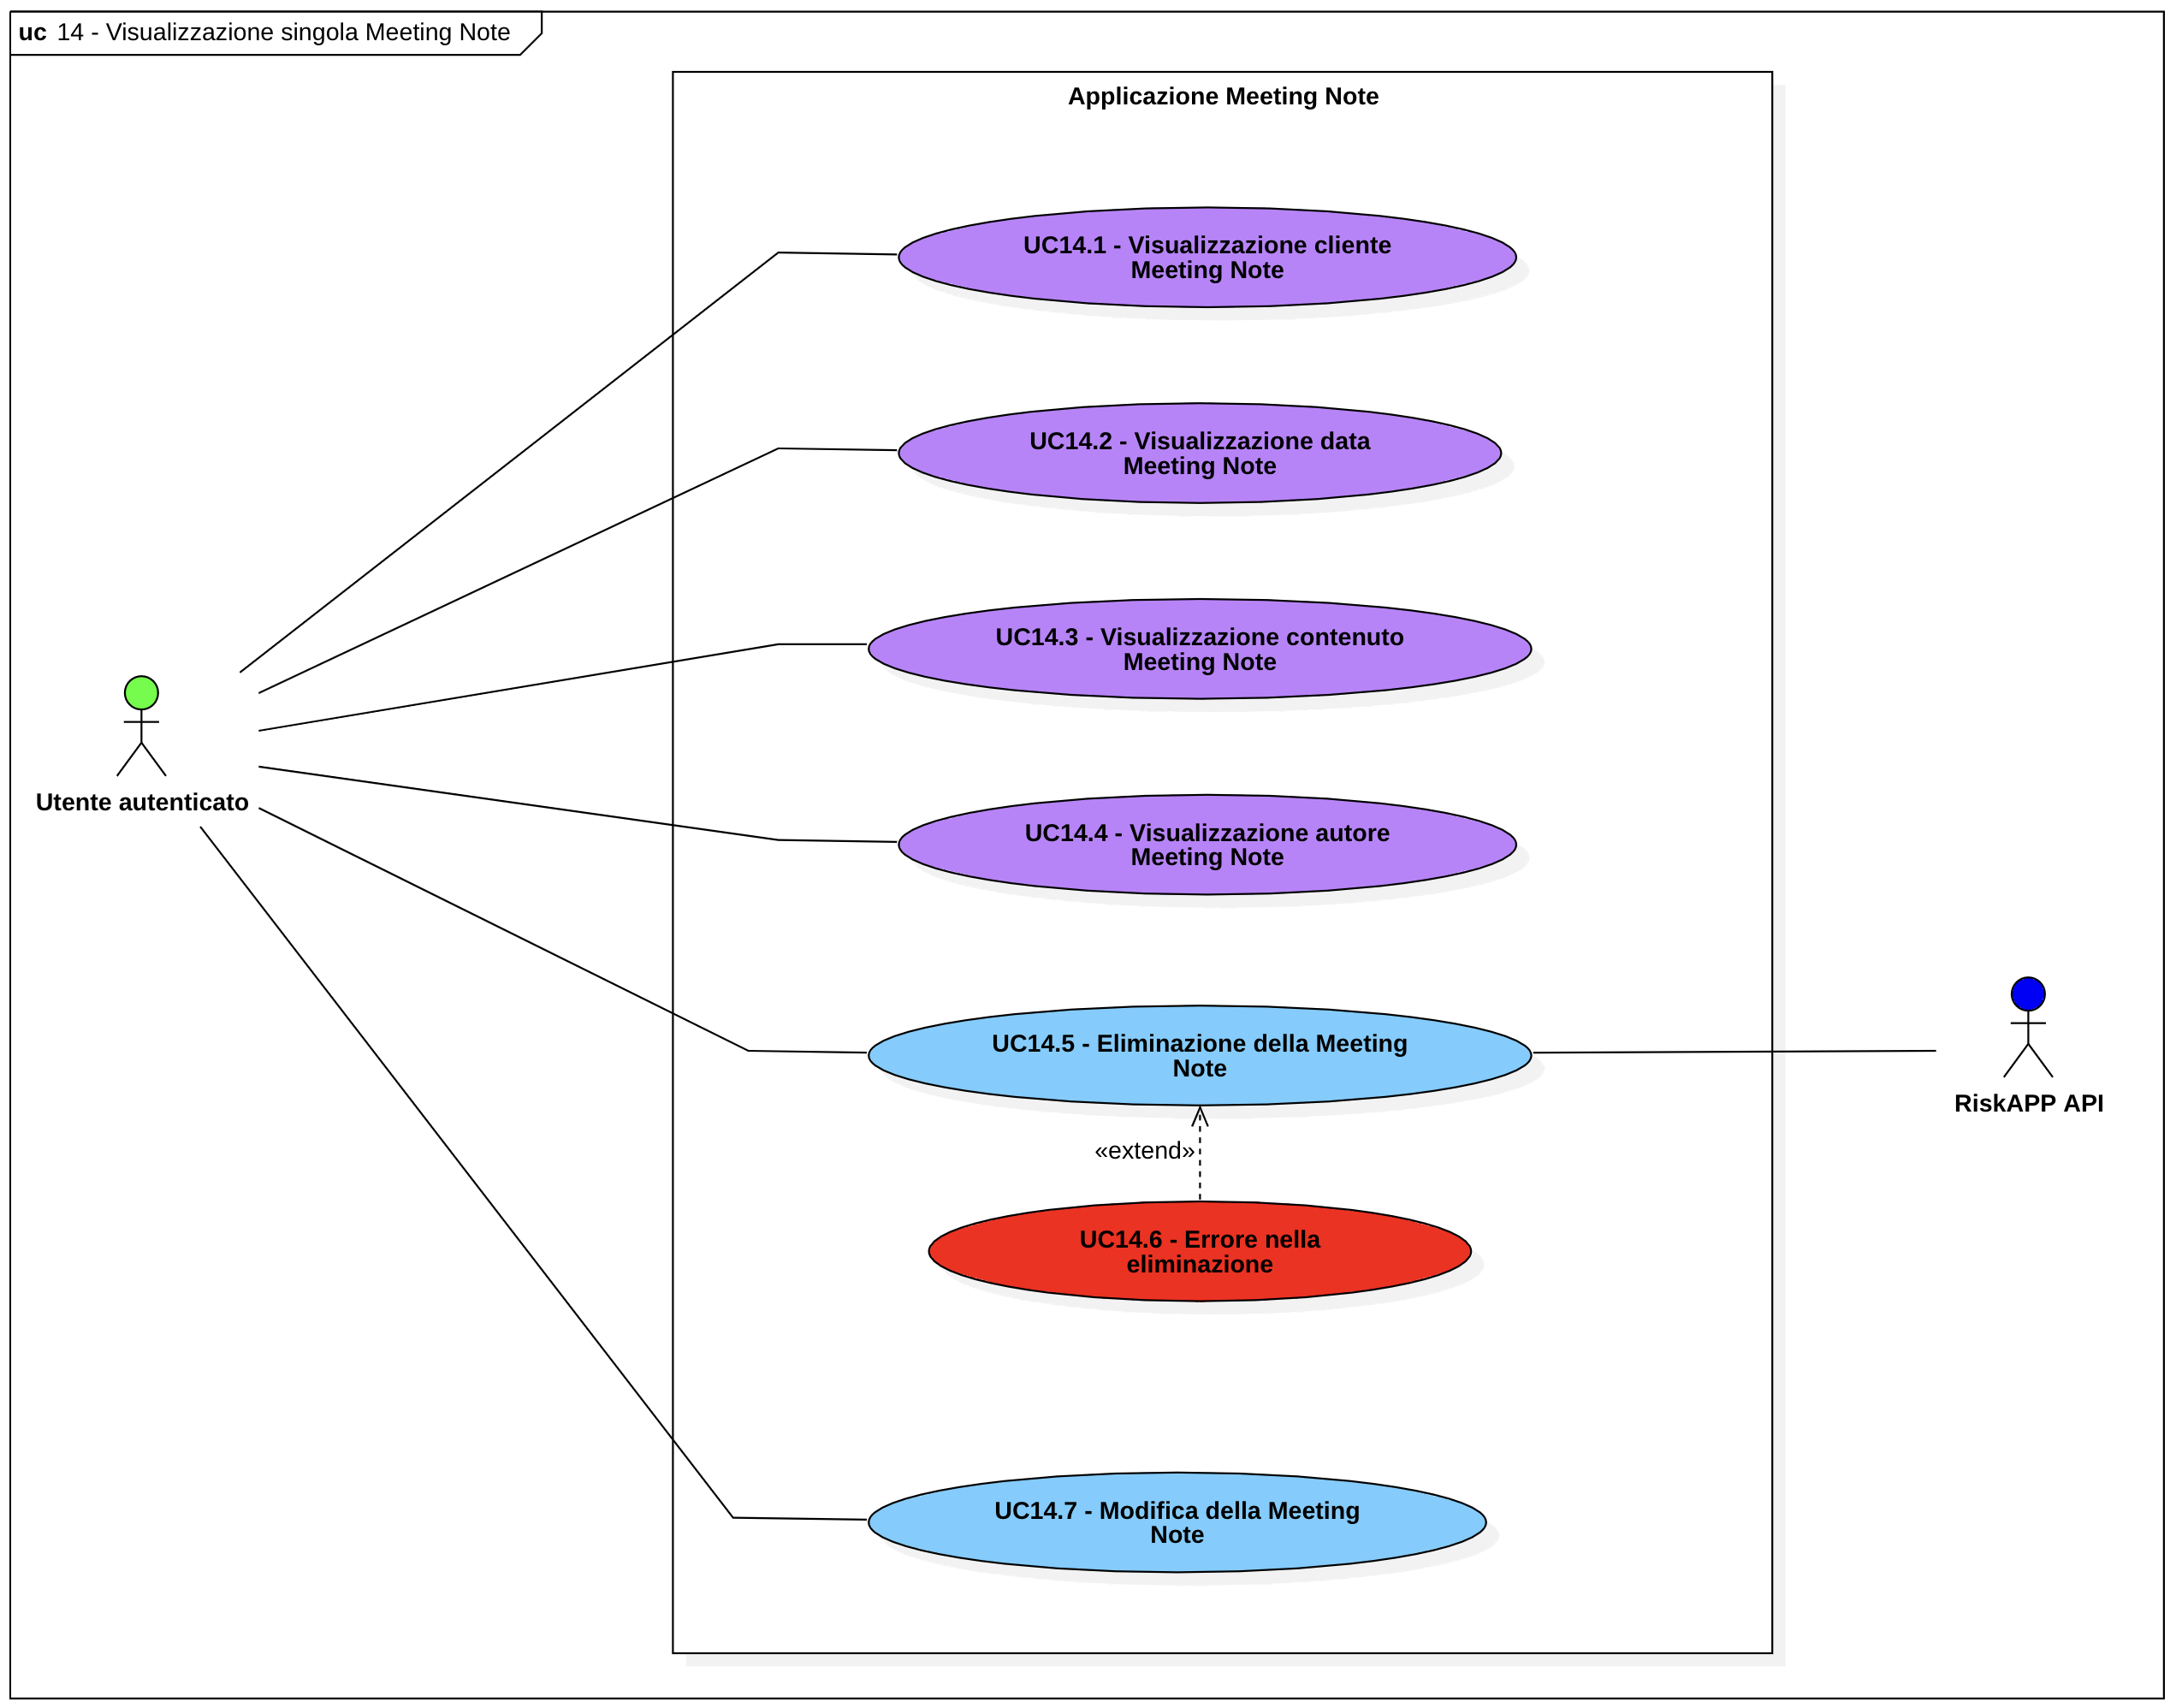
\includegraphics[width=1.0\columnwidth]{usecase/6-uc} 
    \caption{Use Case - Visualizzazione singola Meeting Note}
    \label{fig:uc-meetingnote-details}
\end{figure}

\begin{usecase}{14.1}{Visualizzazione cliente Meeting Note}
    \usecasemainactors{Utente autenticato}
    \usecasepre{L'utente visualizza i dettagli di una singola \gls{meetingnote}\glsoccur}
    \usecasedesc{L'utente vuole visualizzare il \gls{cliente}\glsoccur di una \gls{meetingnote}\glsoccur.}
    \usecasepost{È visualizzabile il \gls{cliente}\glsoccur di una \gls{meetingnote}\glsoccur}
    \usecaseimg{\ref{fig:uc-meetingnote-details}}
    \label{UC14.1}
\end{usecase}

\begin{usecase}{14.2}{Visualizzazione data Meeting Note}
    \usecasemainactors{Utente autenticato}
    \usecasepre{L'utente visualizza i dettagli di una singola \gls{meetingnote}\glsoccur}
    \usecasedesc{L'utente vuole visualizzare la data di una \gls{meetingnote}\glsoccur.}
    \usecasepost{È visualizzabile la data di una \gls{meetingnote}\glsoccur}
    \usecaseimg{\ref{fig:uc-meetingnote-details}}
    \label{UC14.2}
\end{usecase}

\begin{usecase}{14.3}{Visualizzazione contenuto Meeting Note}
    \usecasemainactors{Utente autenticato}
    \usecasepre{L'utente visualizza i dettagli di una singola \gls{meetingnote}\glsoccur}
    \usecasedesc{L'utente vuole visualizzare il contenuto di una \gls{meetingnote}\glsoccur.}
    \usecasepost{È visualizzabile il contenuto di una \gls{meetingnote}\glsoccur}
    \usecaseimg{\ref{fig:uc-meetingnote-details}}
    \label{UC14.3}
\end{usecase}

\begin{usecase}{14.4}{Visualizzazione autore Meeting Note}
    \usecasemainactors{Utente autenticato}
    \usecasepre{L'utente visualizza i dettagli di una singola \gls{meetingnote}\glsoccur}
    \usecasedesc{L'utente vuole visualizzare l'autore di una \gls{meetingnote}\glsoccur.}
    \usecasepost{È visualizzabile l'autore di una \gls{meetingnote}\glsoccur}
    \usecaseimg{\ref{fig:uc-meetingnote-details}}
    \label{UC14.4}
\end{usecase}

\begin{usecase}{14.5}{Eliminazione della Meeting Note}
    \usecasemainactors{Utente autenticato}
    \usecasesecondaryactors{\emph{RiskAPP API}}
    \usecasepre{L'utente visualizza i dettagli di una singola \gls{meetingnote}\glsoccur}
    \usecasedesc{L'utente vuole eliminare la \gls{meetingnote}\glsoccur selezionata.}
    \usecasepost{La \gls{meetingnote}\glsoccur selezionata è stata eliminata}
    \usecasealt{Se l'eliminazione fallisce, si verifica \hyperref[UC14.6]{UC14.6}}
    \usecaseimg{\ref{fig:uc-meetingnote-details}}
    \label{UC14.5}
\end{usecase}

\begin{usecase}{14.6}{Errore nella eliminazione}
    \usecasemainactors{Utente autenticato}
    \usecasesecondaryactors{\emph{RiskAPP API}}
    \usecasepre{L'utente visualizza i dettagli di una singola \gls{meetingnote}\glsoccur}
    \usecasedesc{L'eliminazione della \gls{meetingnote}\glsoccur selezionata fallisce e l'utente viene informato dell'errore; le motivazioni possono essere le seguenti:
        \begin{itemize}
            \item il sistema non è raggiungibile;
            \item token di autenticazione scaduto;
            \item connessione ad internet assente.
        \end{itemize}}
    \usecasepost{La \gls{meetingnote}\glsoccur selezionata non è stata eliminata}
    \usecaseimg{\ref{fig:uc-meetingnote-details}}
    \label{UC14.6}
\end{usecase}

\begin{usecase}{14.7}{Modifica della Meeting Note}
    \usecasemainactors{Utente autenticato}
    \usecasepre{L'utente visualizza i dettagli di una singola \gls{meetingnote}\glsoccur}
    \usecasedesc{L'utente vuole modificare la \gls{meetingnote}\glsoccur selezionata.}
    \usecasepost{La \gls{meetingnote}\glsoccur selezionata è stata modificata}
    \usecaseimg{\ref{fig:uc-meetingnote-details}}
    \label{UC14.7}
\end{usecase}

\newpage

\begin{figure}[!h] 
    \centering 
    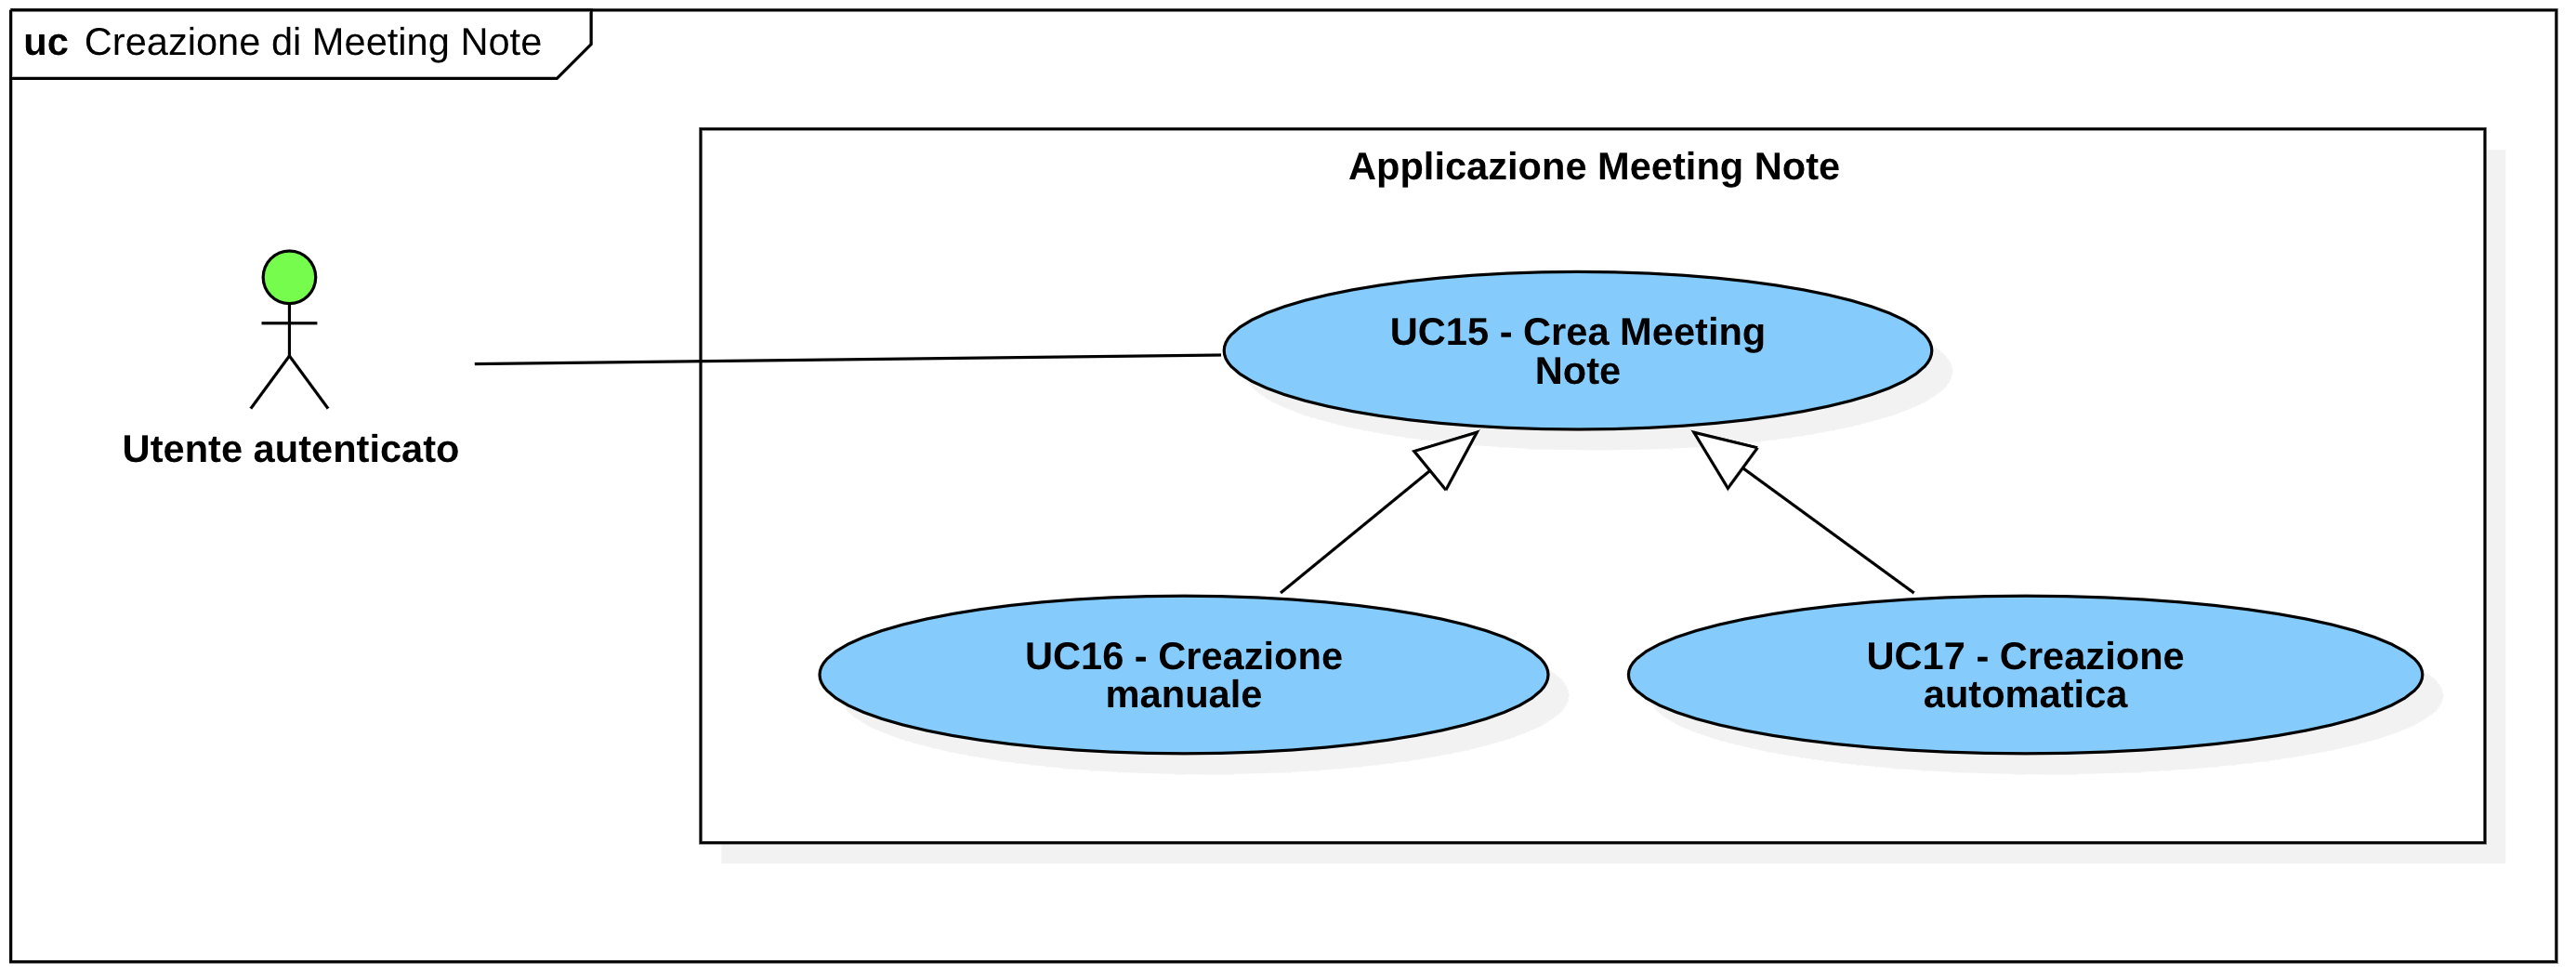
\includegraphics[width=1.0\columnwidth]{usecase/7-uc} 
    \caption{Use Case - Creazione Meeting Note}
    \label{fig:uc-meetingnote-create}
\end{figure}

\begin{usecase}{15}{Crea Meeting Note}
    \usecasemainactors{Utente autenticato}
    \usecasepre{L'utente è autenticato nel sistema}
    \usecasedesc{L'utente vuole creare una nuova \gls{meetingnote}\glsoccur.}
    \usecasepost{Una nuova \gls{meetingnote}\glsoccur è stata creata}
    \usecaseimg{\ref{fig:uc-meetingnote-create}}
    \label{UC15}
\end{usecase}

\begin{usecase}{16}{Creazione manuale}
    \usecasemainactors{Utente autenticato}
    \usecasepre{L'utente è autenticato nel sistema}
    \usecasedesc{L'utente vuole creare manualmente una nuova \gls{meetingnote}\glsoccur.}
    \usecasepost{Una nuova \gls{meetingnote}\glsoccur è stata creata manualmente}
    \usecaseimg{\ref{fig:uc-meetingnote-create}}
    \label{UC16}
\end{usecase}

\begin{usecase}{17}{Creazione automatica}
    \usecasemainactors{Utente autenticato}
    \usecasepre{L'utente è autenticato nel sistema}
    \usecasedesc{L'utente vuole creare automaticamente una nuova \gls{meetingnote}\glsoccur.}
    \usecasepost{Una nuova \gls{meetingnote}\glsoccur è stata creata automaticamente}
    \usecaseimg{\ref{fig:uc-meetingnote-create}}
    \label{UC17}
\end{usecase}

\newpage

\begin{figure}[!h] 
    \centering 
    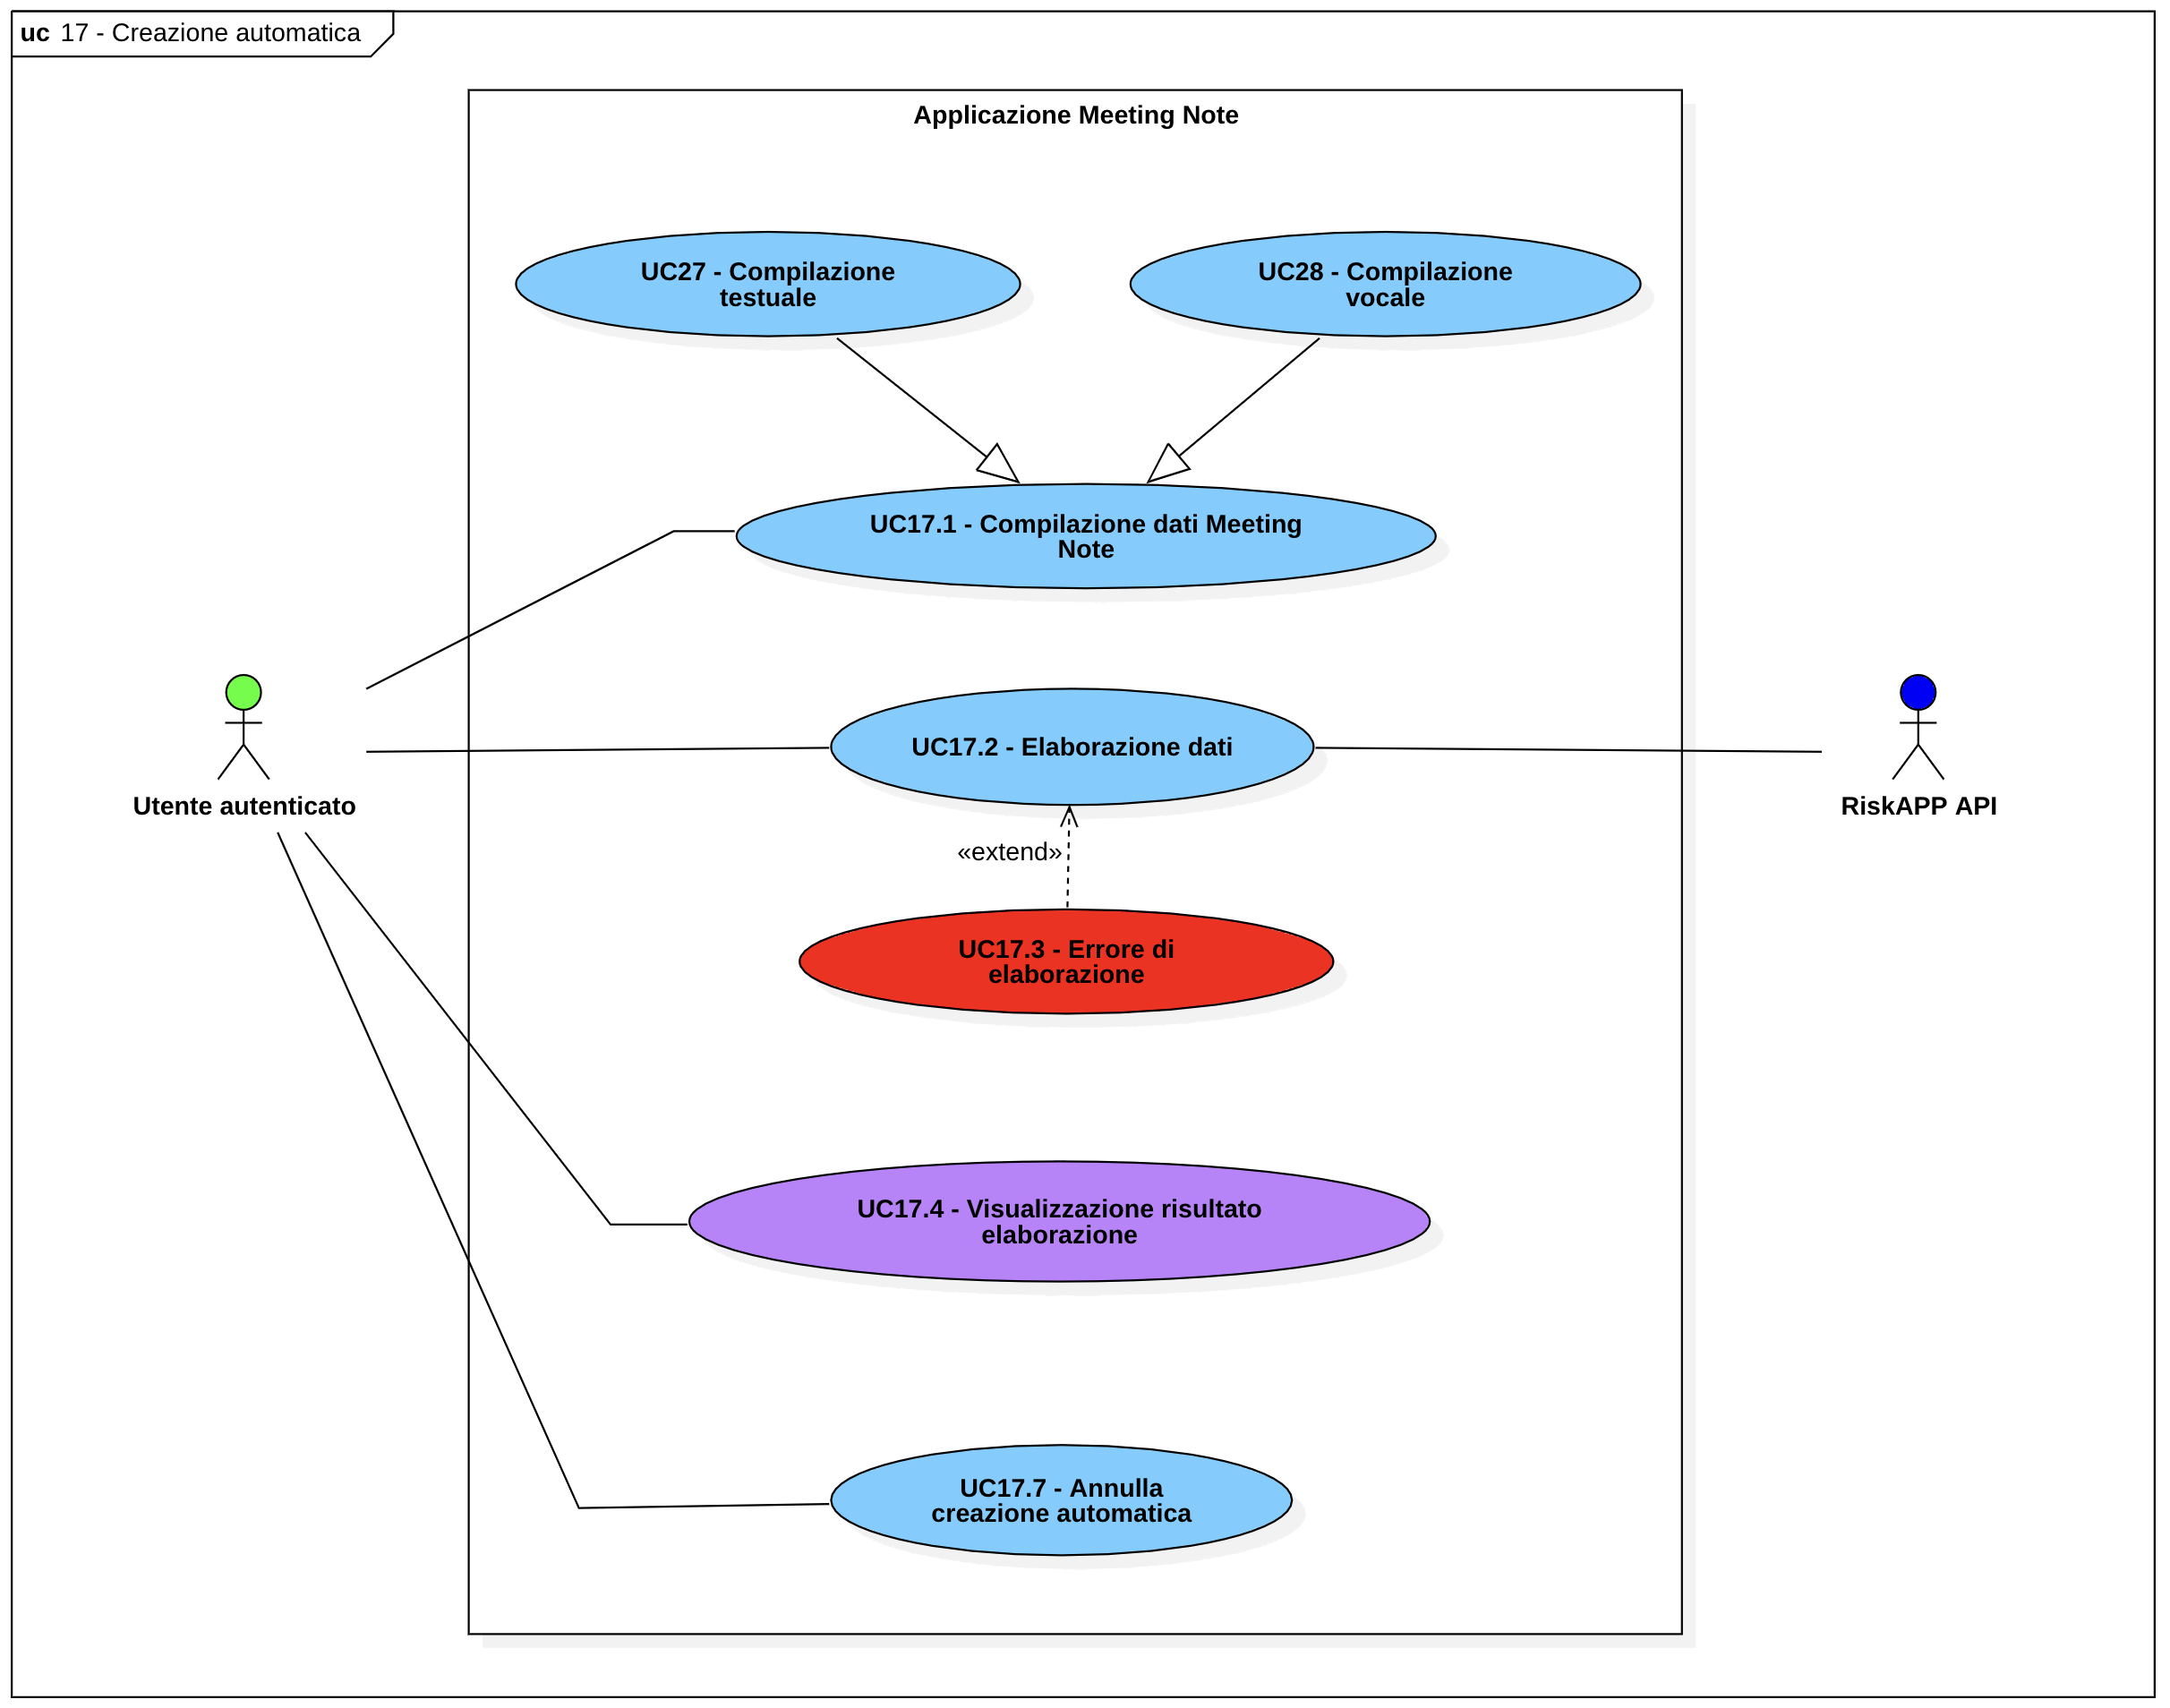
\includegraphics[width=1.0\columnwidth]{usecase/9-uc} 
    \caption{Use Case - Creazione automatica}
    \label{fig:uc-meetingnote-create-automatic}
\end{figure}

\begin{usecase}{17.1}{Compilazione dati Meeting Note}
    \usecasemainactors{Utente autenticato}
    \usecasepre{L'utente vuole creare automaticamente una \gls{meetingnote}\glsoccur}
    \usecasedesc{L'utente compila i dati necessari per la creazione automatica di una \gls{meetingnote}\glsoccur sotto forma di una descrizione testuale.}
    \usecasepost{È stato scritto una breve descrizione testuale con i dati necessari per la creazione automatica di una \gls{meetingnote}\glsoccur}
    \usecaseimg{\ref{fig:uc-meetingnote-create-automatic}}
    \label{UC17.1}
\end{usecase}

\begin{usecase}{17.2}{Elaborazione dati}
    \usecasemainactors{Utente autenticato}
    \usecasesecondaryactors{\emph{RiskAPP API}}
    \usecasepre{L'utente ha compilato i dati necessari per la creazione automatica di una \gls{meetingnote}\glsoccur}
    \usecasedesc{Il testo viene elaborato da una algoritmo di \gls{iag}\glsoccur per estrapolare i dati (cliente, data e contenuto) per la creazione automatica di una \gls{meetingnote}\glsoccur.}
    \usecasepost{I dati (cliente, data e contenuto) per la creazione automatica di una \gls{meetingnote}\glsoccur sono stati estrapolati}
    \usecasealt{Se l'elaborazione fallisce, si verifica \hyperref[UC17.3]{UC17.3}}
    \usecaseimg{\ref{fig:uc-meetingnote-create-automatic}}
    \label{UC17.2}
\end{usecase}

\begin{usecase}{17.3}{Errore elaborazione dati}
    \usecasemainactors{Utente autenticato}
    \usecasesecondaryactors{\emph{RiskAPP API}}
    \usecasepre{L'utente ha compilato i dati necessari per la creazione automatica di una \gls{meetingnote}\glsoccur}
    \usecasedesc{L'elaborazione dei dati per la creazione di una \gls{meetingnote}\glsoccur fallisce e l'utente viene informato dell'errore; le motivazioni possono essere le seguenti:
        \begin{itemize}
            \item l'algoritmo non è stato in grado di estrapolare i dati;
            \item il sistema non è raggiungibile;
            \item token di autenticazione scaduto;
            \item connessione ad internet assente.
        \end{itemize}}
    \usecasepost{I dati per la creazione automatica di una \gls{meetingnote}\glsoccur non sono stati estrapolati}
    \usecaseimg{\ref{fig:uc-meetingnote-create-automatic}}
    \label{UC17.3}
\end{usecase}

\begin{usecase}{17.4}{Visualizzazione risultato elaborazione}
    \usecasemainactors{Utente autenticato}
    \usecasepre{L'algoritmo ha estrapolato i dati per la creazione di una \gls{meetingnote}\glsoccur}
    \usecasedesc{L'utente vuole visualizzare i dati estrapolati dall'algoritmo per la creazione automatica di una \gls{meetingnote}\glsoccur, per accertarsi della loro correttezza.}
    \usecasepost{Sono visualizzabili i dati estrapolati dall'algoritmo per la creazione di una \gls{meetingnote}\glsoccur}
    \usecaseimg{\ref{fig:uc-meetingnote-create-automatic}}
    \label{UC17.4}
\end{usecase}

\newpage

\begin{figure}[!h] 
    \centering 
    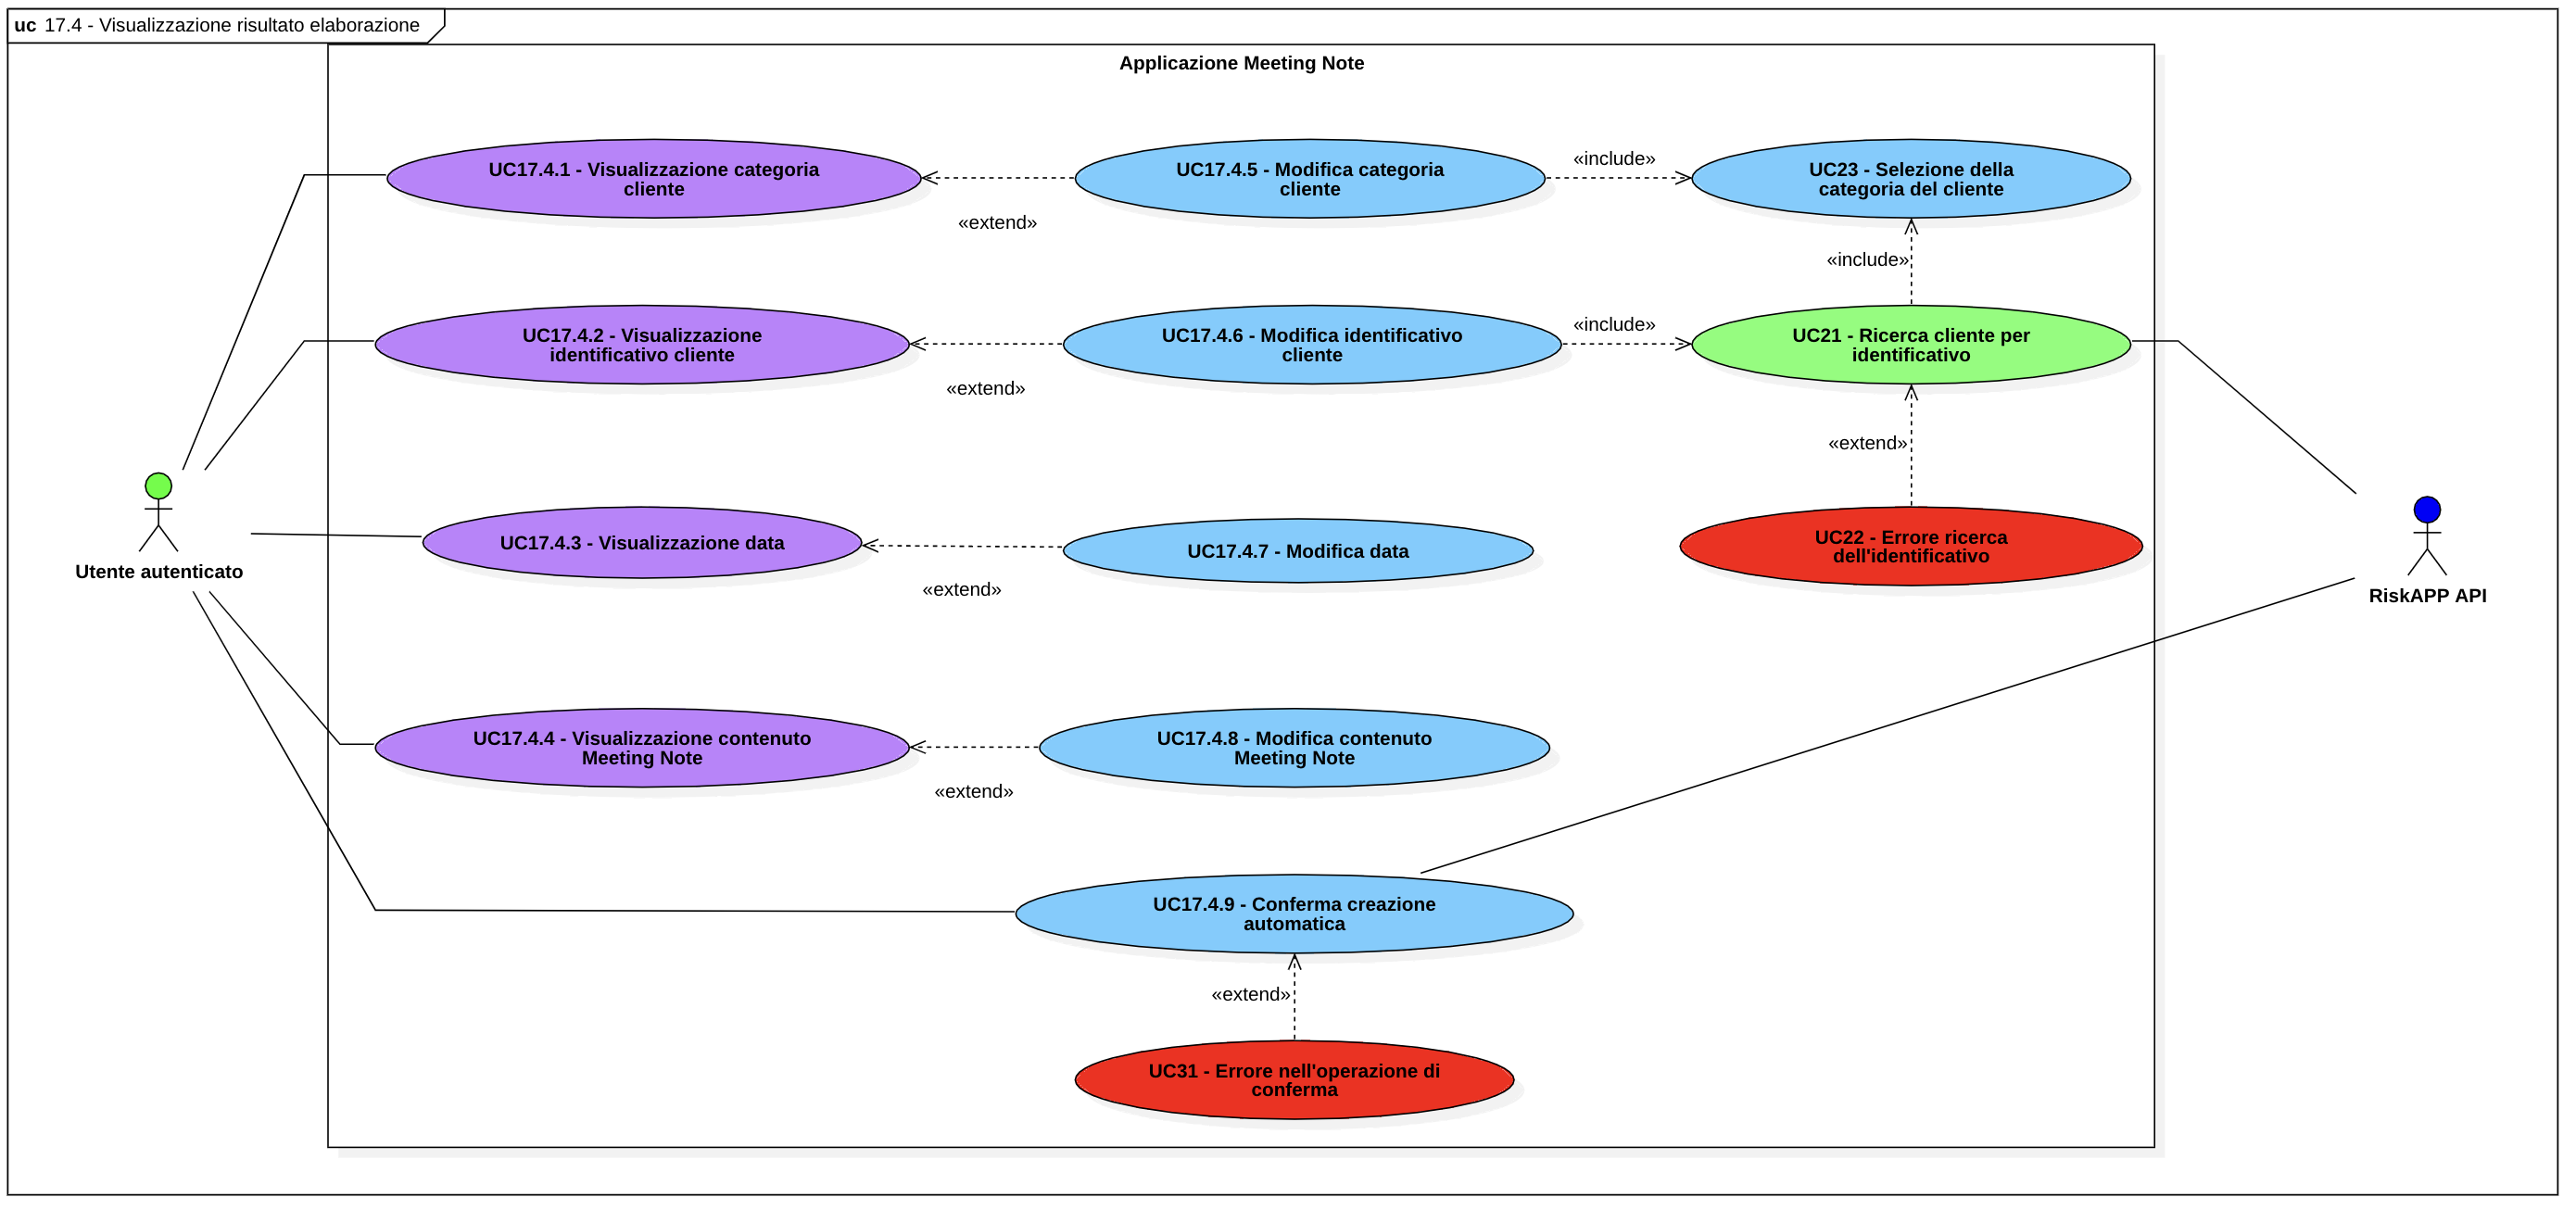
\includegraphics[width=1.0\columnwidth]{usecase/10-uc} 
    \caption{Use Case - Visualizzazione risultato elaborazione}
    \label{fig:uc-meetingnote-create-automatic-result}
\end{figure}

\begin{usecase}{17.4.1}{Visualizzazione categoria cliente}
    \usecasemainactors{Utente autenticato}
    \usecasepre{L'utente visualizza i dati estrapolati dall'algoritmo}
    \usecasedesc{L'utente vuole visualizzare la categoria del \gls{cliente}\glsoccur estrapolato}
    \usecasepost{È visualizzabile la categoria del \gls{cliente}\glsoccur estrapolato}
    \usecaseimg{\ref{fig:uc-meetingnote-create-automatic-result}}
    \label{UC17.4.1}
\end{usecase}

\begin{usecase}{17.4.2}{Visualizzazione identificativo cliente}
    \usecasemainactors{Utente autenticato}
    \usecasepre{L'utente visualizza i dati estrapolati dall'algoritmo}
    \usecasedesc{L'utente vuole visualizzare del \gls{cliente}\glsoccur estrapolato}
    \usecasepost{È visualizzabile l'identificativo del \gls{cliente}\glsoccur estrapolato}
    \usecaseimg{\ref{fig:uc-meetingnote-create-automatic-result}}
    \label{UC17.4.2}
\end{usecase}

\begin{usecase}{17.4.3}{Visualizzazione data}
    \usecasemainactors{Utente autenticato}
    \usecasepre{L'utente visualizza i dati estrapolati dall'algoritmo}
    \usecasedesc{L'utente vuole visualizzare la data estrapolata}
    \usecasepost{È visualizzabile la data estrapolata}
    \usecaseimg{\ref{fig:uc-meetingnote-create-automatic-result}}
    \label{UC17.4.3}
\end{usecase}

\begin{usecase}{17.4.4}{Visualizzazione il contenuto Meeting Note}
    \usecasemainactors{Utente autenticato}
    \usecasepre{L'utente visualizza i dati estrapolati dall'algoritmo}
    \usecasedesc{L'utente vuole visualizzare il contenuto estrapolato}
    \usecasepost{È visualizzabile il contenuto estrapolato}
    \usecaseimg{\ref{fig:uc-meetingnote-create-automatic-result}}
    \label{UC17.4.4}
\end{usecase}

\begin{usecase}{17.4.5}{Modifica categoria cliente}
    \usecasemainactors{Utente autenticato}
    \usecasepre{L'utente visualizza la categoria del \gls{cliente}\glsoccur estrapolato}
    \usecasedesc{L'utente modifica la categoria del \gls{cliente}\glsoccur}
    \usecasepost{La categoria del \gls{cliente}\glsoccur è stato modificato}
    \usecaseimg{\ref{fig:uc-meetingnote-create-automatic-result}}
    \label{15.4.5}
\end{usecase}

\begin{usecase}{17.4.6}{Modifica identificativo cliente}
    \usecasemainactors{Utente autenticato}
    \usecasepre{L'utente visualizza l'identificativo del \gls{cliente}\glsoccur estrapolato}
    \usecasedesc{L'utente modifica l'identificativo del \gls{cliente}\glsoccur}
    \usecasepost{L'identificativo del \gls{cliente}\glsoccur è stato modificato}
    \usecaseimg{\ref{fig:uc-meetingnote-create-automatic-result}}
    \label{15.4.6}
\end{usecase}

\begin{usecase}{17.4.7}{Modifica data}
    \usecasemainactors{Utente autenticato}
    \usecasepre{L'utente visualizza la data estrapolata}
    \usecasedesc{L'utente modifica la data}
    \usecasepost{La data è stata modificata}
    \usecaseimg{\ref{fig:uc-meetingnote-create-automatic-result}}
    \label{15.4.7}
\end{usecase}

\begin{usecase}{17.4.8}{Modifica contenuto Meeting Note}
    \usecasemainactors{Utente autenticato}
    \usecasepre{L'utente visualizza il contenuto estrapolato}
    \usecasedesc{L'utente modifica il contenuto}
    \usecasepost{Il contenuto è stato modificato}
    \usecaseimg{\ref{fig:uc-meetingnote-create-automatic-result}}
    \label{15.4.8}
\end{usecase}

\begin{usecase}{17.4.9}{Conferma creazione automatica}
    \usecasemainactors{Utente autenticato}
    \usecasepre{L'utente vuole creare automaticamente una \gls{meetingnote}\glsoccur}
    \usecasedesc{L'utente conferma la creazione automatica di una \gls{meetingnote}\glsoccur.}
    \usecasepost{Una nuova \gls{meetingnote}\glsoccur è stata creata automaticamente}
    \usecasealt{Se la conferma fallisce, si verifica \hyperref[UC31]{UC31}}
    \usecaseimg{\ref{fig:uc-meetingnote-create-automatic-result}}
    \label{15.4.9}
\end{usecase}

\begin{usecase}{17.5}{Annulla creazione automatica}
    \usecasemainactors{Utente autenticato}
    \usecasepre{L'utente é in fase di creazione automatica di una \gls{meetingnote}\glsoccur}
    \usecasedesc{L'utente annulla la creazione automatica di una \gls{meetingnote}\glsoccur.}
    \usecasepost{Non è stata creata una nuova \gls{meetingnote}\glsoccur}
    \usecaseimg{\ref{fig:uc-meetingnote-create-automatic}}
    \label{UC17.5}
\end{usecase}

\newpage

\begin{figure}[!h] 
    \centering 
    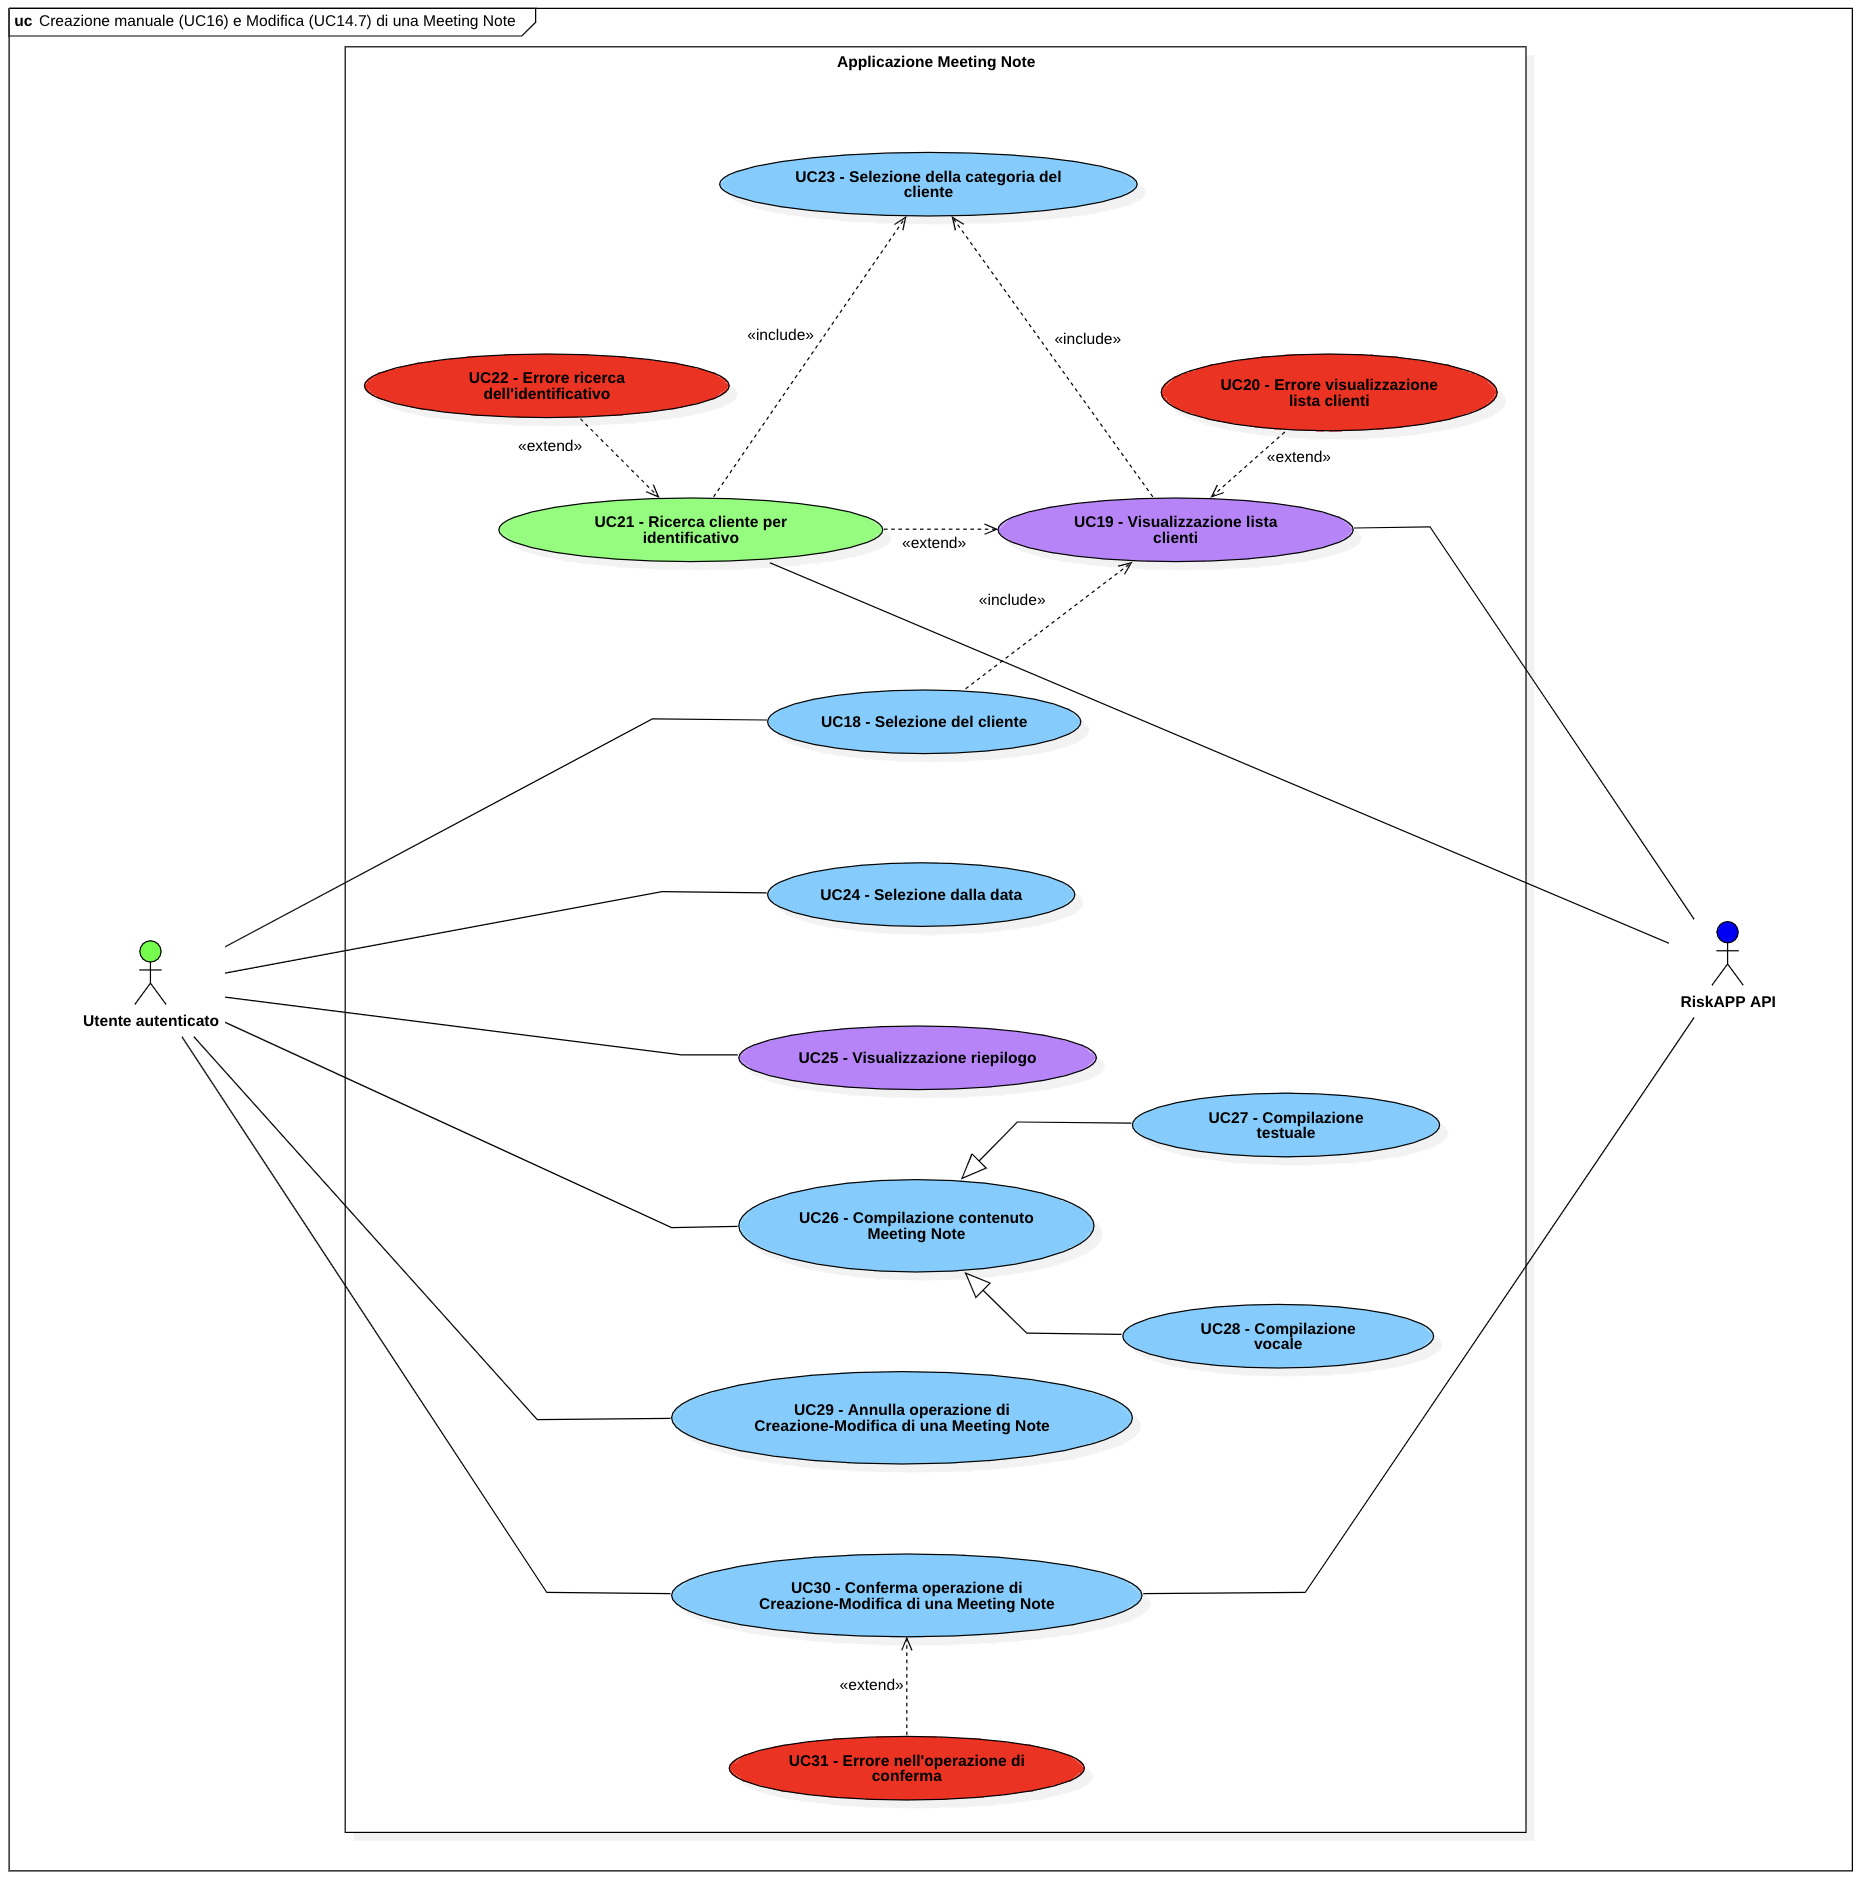
\includegraphics[width=1.0\columnwidth]{usecase/8-uc} 
    \caption{Use Case - Creazione manuale (\hyperref[UC16]{UC16}) e Modifica (\hyperref[UC14.7]{UC14.7}) di una Meeting Note}
    \label{fig:uc-meetingnote-create-manual}
\end{figure}

\noindent Per la creazione manuale (\hyperref[UC16]{UC16}) e modifica (\hyperref[UC14.7]{UC14.7}) di una \gls{meetingnote}\glsoccur sono stati individuati i seguenti \glspl{usecase}\glsoccur, che sono in comune tra le due funzionalità sopra citate, in quanto condividono la stessa sequenza di azioni, e dunque di attori principali, secondari, precondizioni e postcondizioni.

\begin{usecase}{18}{Selezione del cliente}
    \usecasemainactors{Utente autenticato}
    \usecasepre{L'utente vuole creare manualmente o modificare una \gls{meetingnote}\glsoccur}
    \usecasedesc{L'utente deve selezionare un \gls{cliente}\glsoccur per la creazione o la modifica di una \gls{meetingnote}\glsoccur.}
    \usecasepost{Il \gls{cliente}\glsoccur è stato selezionato}
    \usecaseimg{\ref{fig:uc-meetingnote-create-manual}}
    \label{UC18}
\end{usecase}

\begin{usecase}{19}{Visualizzazione lista clienti}
    \usecasemainactors{Utente autenticato}
    \usecasesecondaryactors{\emph{RiskAPP API}}
    \usecasepre{L'utente ha selezionato la categoria del \gls{cliente}\glsoccur}
    \usecasedesc{L'utente vuole visualizzare la lista di tutti i \glspl{cliente}\glsoccur della categoria selezionata.}
    \usecasepost{È visualizzabile la lista dei \glspl{cliente}\glsoccur filtrata per categoria}
    \usecasealt{Se la visualizzazione fallisce, si verifica \hyperref[UC20]{UC20}}
    \usecaseimg{\ref{fig:uc-meetingnote-create-manual}}
    \label{UC19}
\end{usecase}

\begin{usecase}{20}{Errore visualizzazione lista clienti}
    \usecasemainactors{Utente autenticato}
    \usecasesecondaryactors{\emph{RiskAPP API}}
    \usecasepre{L'utente ha selezionato la categoria del \gls{cliente}\glsoccur}
    \usecasedesc{La visualizzazione della lista dei \glspl{cliente}\glsoccur fallisce e l'utente viene informato dell'errore; le motivazioni possono essere le seguenti:
        \begin{itemize}
            \item la lista è vuota;
            \item il sistema non è raggiungibile;
            \item token di autenticazione scaduto;
            \item connessione ad internet assente.
        \end{itemize}}
    \usecasepost{Non è visualizzabile la lista dei \glspl{cliente}\glsoccur filtrata per categoria}
    \usecaseimg{\ref{fig:uc-meetingnote-create-manual}}
    \label{UC20}
\end{usecase}

\begin{usecase}{21}{Ricerca cliente per identificativo}
    \usecasemainactors{Utente autenticato}
    \usecasesecondaryactors{\emph{RiskAPP API}}
    \usecasepre{L'utente ha selezionato la categoria del \gls{cliente}\glsoccur}
    \usecasedesc{L'utente effettua una ricerca per identificativo del \gls{cliente}\glsoccur.}
    \usecasepost{L'identificativo del \gls{cliente}\glsoccur è stato trovato}
    \usecasealt{Se la ricerca fallisce, si verifica \hyperref[UC22]{UC22}}
    \usecaseimg{\ref{fig:uc-meetingnote-create-manual}}
    \label{UC21}
\end{usecase}

\begin{usecase}{22}{Errore ricerca dell'identificativo}
    \usecasemainactors{Utente autenticato}
    \usecasesecondaryactors{\emph{RiskAPP API}}
    \usecasepre{L'utente ha effettuato una ricerca per identificativo del \gls{cliente}\glsoccur}
    \usecasedesc{La ricerca dell'identificativo del \gls{cliente}\glsoccur fallisce e l'utente viene informato dell'errore; le motivazioni possono essere le seguenti:
        \begin{itemize}
            \item la lista risultante è vuota;
            \item il sistema non è raggiungibile;
            \item token di autenticazione scaduto;
            \item connessione ad internet assente.
        \end{itemize}}
    \usecasepost{L'identificativo del \gls{cliente}\glsoccur non è stato trovato}
    \usecaseimg{\ref{fig:uc-meetingnote-create-manual}}
    \label{UC22}
\end{usecase}

\begin{usecase}{23}{Selezione della categoria del cliente}
    \usecasemainactors{Utente autenticato}
    \usecasepre{L'utente è in fase di creazione o modifica}
    \usecasedesc{L'utente seleziona la categoria del \gls{cliente}\glsoccur per filtrare la lista dei \glspl{cliente}\glsoccur e/o la ricerca dell'identificativo.}
    \usecasepost{La categoria del \gls{cliente}\glsoccur è stata selezionata}
    \usecaseimg{\ref{fig:uc-meetingnote-create-manual}}
    \label{UC23}
\end{usecase}

\begin{usecase}{24}{Selezione della data}
    \usecasemainactors{Utente autenticato}
    \usecasepre{L'utente vuole creare manualmente o modificare una \gls{meetingnote}\glsoccur}
    \usecasedesc{L'utente deve selezionare una data, in cui è avvenuto l'incontro, per la creazione o la modifica di una \gls{meetingnote}\glsoccur.}
    \usecasepost{La data dell'incontro è stata selezionata}
    \usecaseimg{\ref{fig:uc-meetingnote-create-manual}}
    \label{UC24}
\end{usecase}

\begin{usecase}{25}{Visualizzazione riepilogo}
    \usecasemainactors{Utente autenticato}
    \usecasepre{L'utente ha selezionato un \gls{cliente}\glsoccur e una data}
    \usecasedesc{Viene visualizzato il riepilogo dei dati selezionati.}
    \usecasepost{È visualizzabile il riepilogo dei dati selezionati}
    \usecaseimg{\ref{fig:uc-meetingnote-create-manual}}
    \label{UC25}
\end{usecase}

\newpage

\begin{figure}[!h] 
    \centering 
    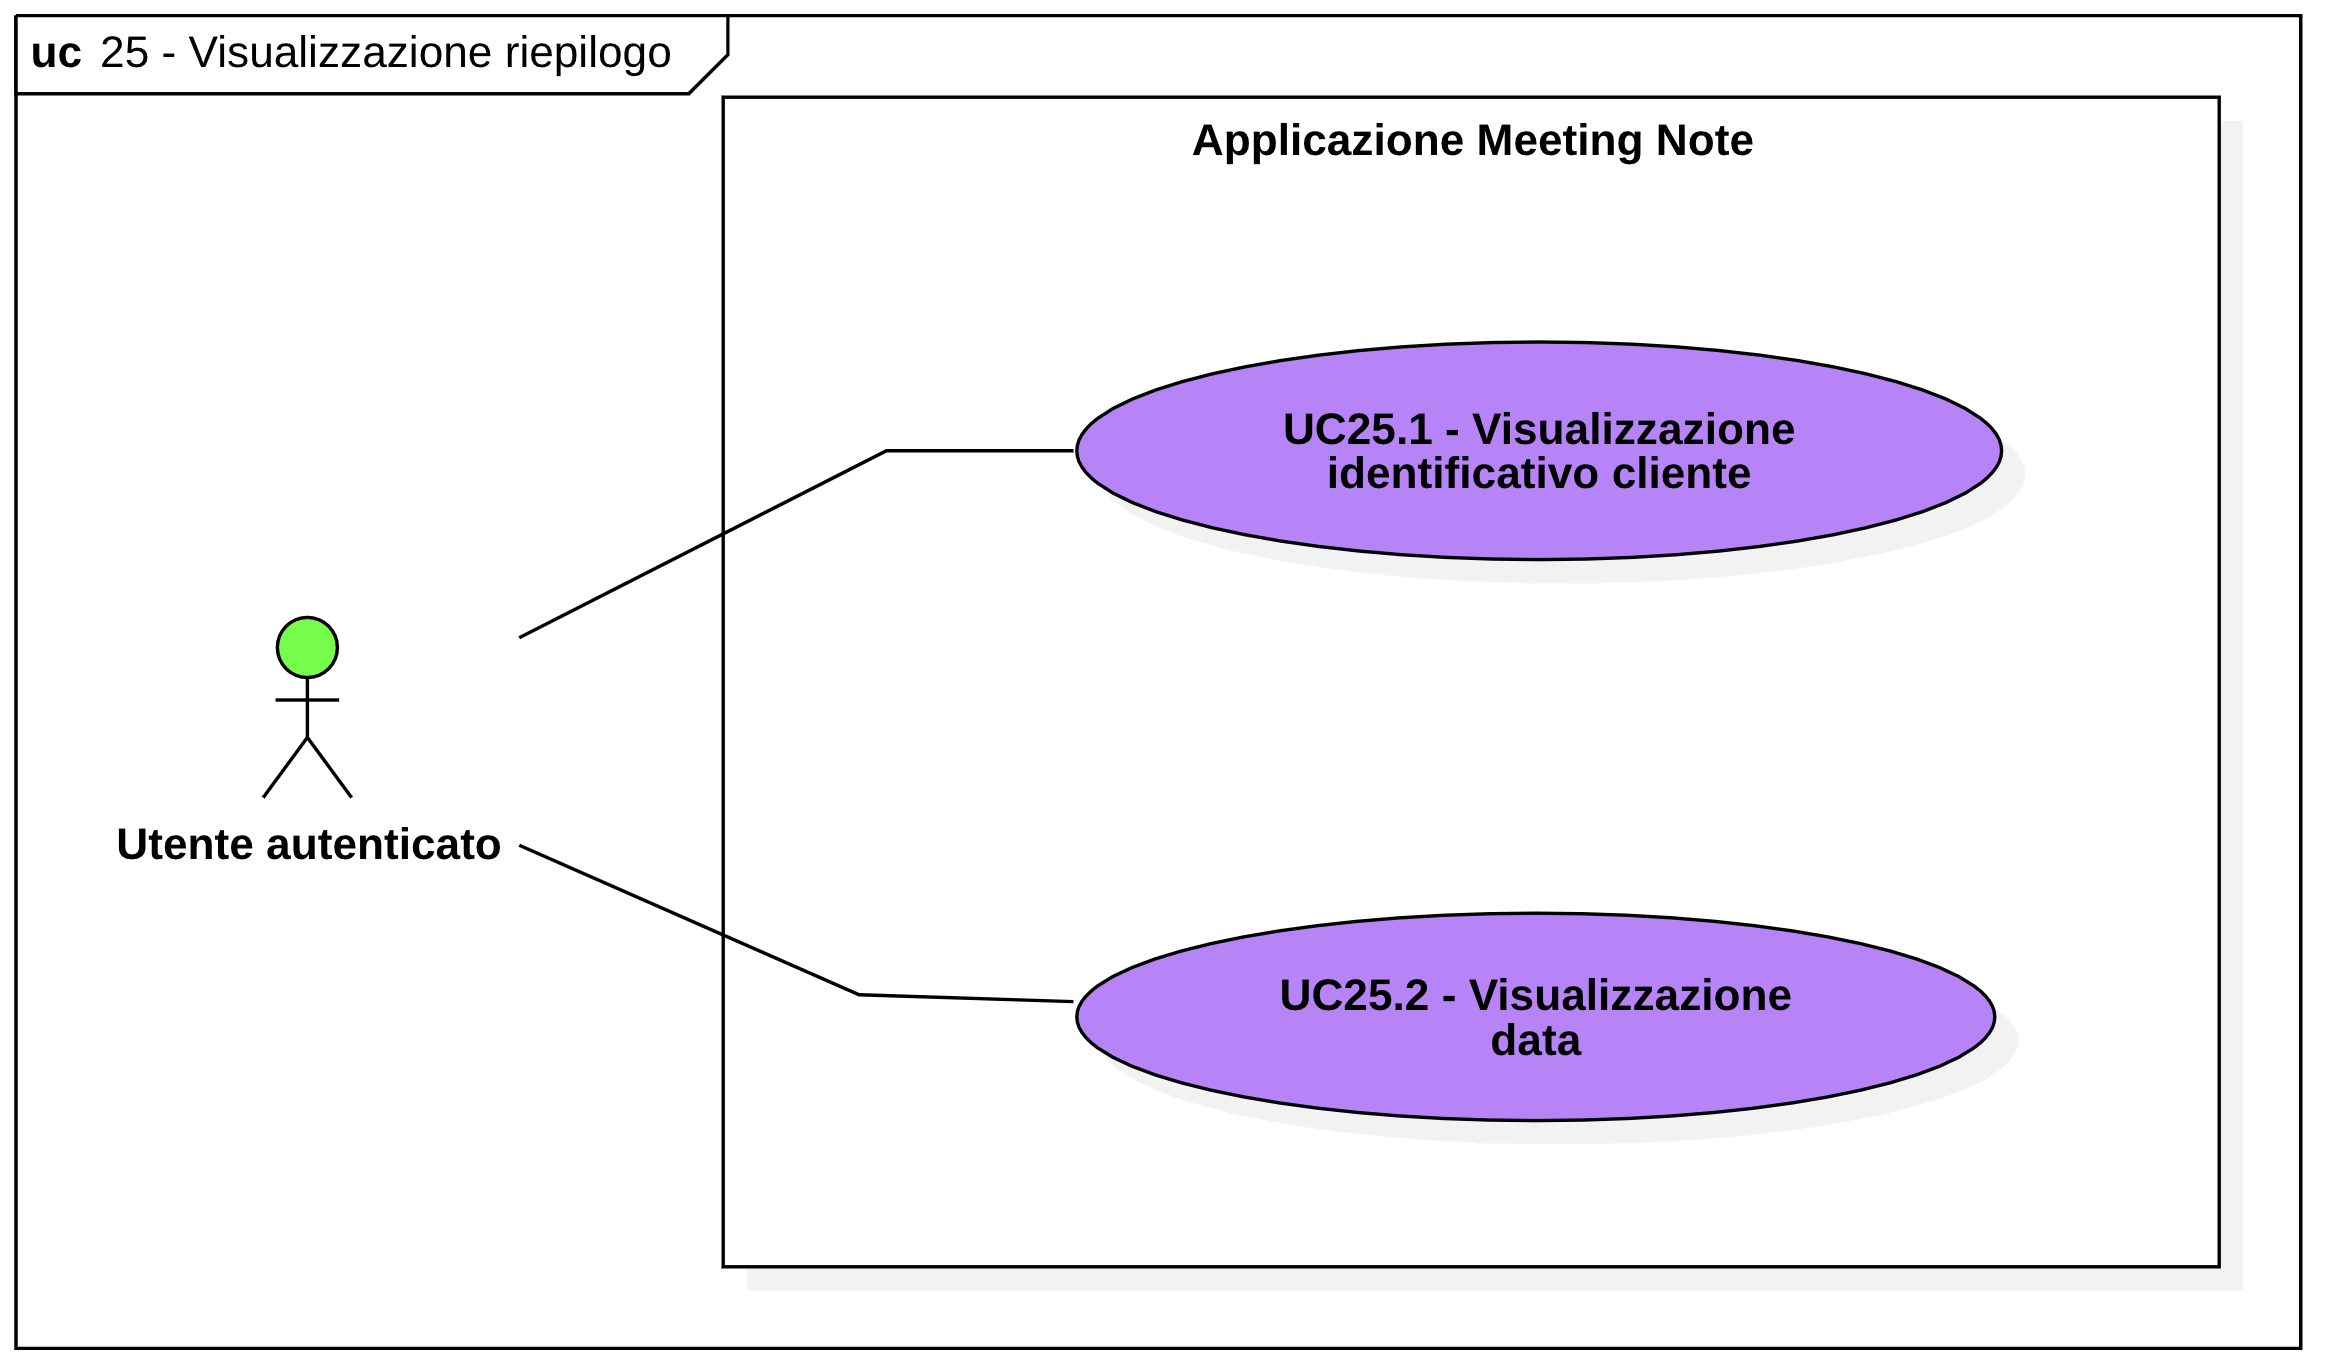
\includegraphics[width=1.0\columnwidth]{usecase/11-uc} 
    \caption{Use Case - Visualizzazione riepilogo}
    \label{fig:uc-meetingnote-create-manual-result}
\end{figure}

\begin{usecase}{25.1}{Visualizzazione identificativo cliente}
    \usecasemainactors{Utente autenticato}
    \usecasepre{L'utente visualizza il riepilogo}
    \usecasedesc{Viene visualizzato l'identificativo del \gls{cliente}\glsoccur selezionato.}
    \usecasepost{È visualizzabile l'identificativo del \gls{cliente}\glsoccur selezionato}
    \usecaseimg{\ref{fig:uc-meetingnote-create-manual-result}}
    \label{UC25.1}
\end{usecase}

\begin{usecase}{25.2}{Visualizzazione data}
    \usecasemainactors{Utente autenticato}
    \usecasepre{L'utente visualizza il riepilogo}
    \usecasedesc{Viene visualizzata la data selezionata.}
    \usecasepost{È visualizzabile la data selezionata}
    \usecaseimg{\ref{fig:uc-meetingnote-create-manual-result}}
    \label{UC25.2}
\end{usecase}

\begin{usecase}{26}{Compilazione contenuto Meeting Note}
    \usecasemainactors{Utente autenticato}
    \usecasepre{L'utente vuole creare manualmente o modificare una \gls{meetingnote}\glsoccur}
    \usecasedesc{L'utente deve compilare il contenuto della \gls{meetingnote}\glsoccur.}
    \usecasepost{Il contenuto della \gls{meetingnote}\glsoccur è compilato}
    \usecaseimg{\ref{fig:uc-meetingnote-create-manual}}
    \label{UC26}
\end{usecase}

\begin{usecase}{27}{Compilazione testuale}
    \usecasemainactors{Utente autenticato}
    \usecasepre{L'utente deve compilare il contenuto della \gls{meetingnote}\glsoccur}
    \usecasedesc{L'utente deve compilare il contenuto della \gls{meetingnote}\glsoccur con l'ausilio della tastiera.}
    \usecasepost{Il contenuto della \gls{meetingnote}\glsoccur è stato compilato con l'ausilio della tastiera}
    \usecaseimg{\ref{fig:uc-meetingnote-create-manual}}
    \label{UC27}
\end{usecase}

\begin{usecase}{28}{Compilazione vocale}
    \usecasemainactors{Utente autenticato}
    \usecasepre{L'utente deve compilare il contenuto della \gls{meetingnote}\glsoccur}
    \usecasedesc{L'utente deve compilare il contenuto della \gls{meetingnote}\glsoccur attraverso la dettatura vocale.}
    \usecasepost{Il contenuto della \gls{meetingnote}\glsoccur è stato compilato attraverso la dettatura vocale}
    \usecaseimg{\ref{fig:uc-meetingnote-create-manual}}
    \label{UC28}
\end{usecase}

\begin{usecase}{29}{Annulla operazione di Creazione-Modifica di una Meeting Note}
    \usecasemainactors{Utente autenticato}
    \usecasepre{L'utente ha selezionato: \gls{cliente}\glsoccur, data e compilato il contenuto della \gls{meetingnote}\glsoccur}
    \usecasedesc{L'utente vuole annullare l'operazione di creazione o modifica di una \gls{meetingnote}\glsoccur.}
    \usecasepost{L'operazione di creazione o modifica di una \gls{meetingnote}\glsoccur è annullata}
    \usecaseimg{\ref{fig:uc-meetingnote-create-manual}}
    \label{UC29}
\end{usecase}

\begin{usecase}{30}{Conferma operazione di Creazione-Modifica di una Meeting Note}
    \usecasemainactors{Utente autenticato}
    \usecasesecondaryactors{\emph{RiskAPP API}}
    \usecasepre{L'utente ha selezionato: \gls{cliente}\glsoccur, data e compilato il contenuto della \gls{meetingnote}\glsoccur}
    \usecasedesc{L'utente vuole confermare l'operazione di creazione o modifica di una \gls{meetingnote}\glsoccur.}
    \usecasepost{L'operazione di creazione o modifica di una \gls{meetingnote}\glsoccur è confermata}
    \usecasealt{Se la conferma fallisce, si verifica \hyperref[UC31]{UC31}}
    \usecaseimg{\ref{fig:uc-meetingnote-create-manual}}
    \label{UC30}
\end{usecase}

\begin{usecase}{31}{Errore nell'operazione di conferma}
    \usecasemainactors{Utente autenticato}
    \usecasesecondaryactors{\emph{RiskAPP API}}
    \usecasepre{L'utente ha confermato l'operazione di creazione o modifica di una \gls{meetingnote}\glsoccur}
    \usecasedesc{La conferma dell'operazione di creazione o modifica della \gls{meetingnote}\glsoccur fallisce e l'utente viene informato dell'errore; le motivazioni possono essere le seguenti:
        \begin{itemize}
            \item il sistema non è raggiungibile;
            \item token di autenticazione scaduto;
            \item connessione ad internet assente.
        \end{itemize}}
    \usecasepost{La conferma dell'operazione di creazione o modifica di una \gls{meetingnote}\glsoccur è fallita}
    \usecaseimg{\ref{fig:uc-meetingnote-create-manual}}
    \label{UC31}
\end{usecase}

\clearpage

\section{Tracciamento dei requisiti}

Da un'attenta analisi dei requisiti e dei casi d'uso effettuata sul progetto è stata stilata la tabella che traccia i requisiti.\\
Sono stati individuati diversi tipi di requisiti e si è quindi fatto utilizzo di un codice identificativo per distinguerli.\\
Il codice dei requisiti è così strutturato R(F/Q/V)(N/D/O) dove:
\begin{enumerate}
	\item[R =] requisito
    \item[F =] funzionale
    \item[Q =] qualitativo
    \item[V =] di vincolo
    \item[N =] obbligatorio (necessario)
    \item[D =] desiderabile
    \item[Z =] opzionale
\end{enumerate}

Di seguito sono riportate le tabelle che raccolgono, per tipologia, i requisiti individuati.\\
\begin{itemize}
    \item \textbf{Requisiti funzionali}: descrivono le funzionalità offerte dal prodotto software. Si faccia riferimento alle tabelle \ref{tab:requisiti-funzionali-1}, \ref{tab:requisiti-funzionali-2}, \ref{tab:requisiti-funzionali-3}, \ref{tab:requisiti-funzionali-4};
    \item \textbf{Requisiti qualitativi}: descrivono le caratteristiche qualitative che il prodotto software deve possedere. Si faccia riferimento alla tabella \ref{tab:requisiti-qualitativi};
    \item \textbf{Requisiti di vincolo}: descrivono i vincoli che il prodotto software deve rispettare. Si faccia riferimento alla tabella \ref{tab:requisiti-vincolo}.
\end{itemize}

\clearpage

\begin{table}%
\caption{Tabella del tracciamento dei requisti funzionali - 1}
\label{tab:requisiti-funzionali-1}
\begin{tabularx}{\textwidth}{lXl}
\hline\hline
\textbf{Requisito} & \textbf{Descrizione} & \textbf{Use Case}\\
\hline
RFN-1 \label{RFN-1} & Il sistema permette di effettuare l'autenticazione & \hyperref[UC01]{UC01} \\
\hline
RFN-2 \label{RFN-2} & Il sistema permette di inserire le credenziali (\emph{username} e \emph{password}) per effettuare l'autenticazione & \hyperref[UC02]{UC02} \\
\hline
RFN-3 \label{RFN-3} & Il sistema permette il riconoscimento biometrico per effettuare l'autenticazione & \hyperref[UC03]{UC03} \\
\hline
% INSERIRE RFN CHE SPECIFICA IL FALLIMENTO DELL'AUTENTICAZIONE (IN TEORIA CI SONO ALTRI CASI SIMILI, DA SPECIFICARE ANALOGAMENTE)
RFN-4 \label{RFN-4} & Il sistema deve notificare l'utente in caso di inserimento di credenziali errate & \hyperref[UC04]{UC04} \\ % \hyperref[UC08.8]{UC08.8}
\hline
RFN-5 \label{RFN-5} & Il sistema deve notificare l'utente in caso in cui il sistema, ovvero la piattaforma \emph{RiskAPP} non sia raggiungibile & \hyperref[UC04]{UC04} \\ %, \hyperref[UC06]{UC06}, \hyperref[UC07.6]{UC07.6}, \hyperref[UC08.8]{UC08.8}, \hyperref[UC09]{UC09}, \hyperref[UC13]{UC13}, \hyperref[UC14.6]{UC14.6}, \hyperref[UC17.3]{UC17.3}, \hyperref[UC20]{UC20}, \hyperref[UC22]{UC22}, \hyperref[UC31]{UC31} 
\hline
RFN-6 \label{RFN-6} & Il sistema deve permettere all'utente, in caso in cui il riconoscimento biometrico fallisca, di poter inserire le credenziali manualmente & \hyperref[UC04]{UC04} \\
\hline
RFN-7 \label{RFN-7} & Il sistema deve notificare l'utente in caso di connessione internet assente & \hyperref[UC04]{UC04} \\ %, \hyperref[UC06]{UC06}, \hyperref[UC07.6]{UC07.6}, \hyperref[UC08.8]{UC08.8}, \hyperref[UC09]{UC09}, \hyperref[UC13]{UC13}, \hyperref[UC14.6]{UC14.6}, \hyperref[UC17.3]{UC17.3}, \hyperref[UC20]{UC20}, \hyperref[UC22]{UC22}, \hyperref[UC31]{UC31} 
\hline
RFN-8 \label{RFN-8} & Il sistema permette di visualizzare la lista di \emph{Meeting Note} & \hyperref[UC05]{UC05} \\
\hline
RFN-9 \label{RFN-9} & Il sistema permette di visualizzare i clienti di ciascuna \emph{Meeting Note} nella lista & \hyperref[UC05.1]{UC05.1} \\
\hline
RFN-10 \label{RFN-10} & Il sistema permette di visualizzare la data dell'incontro di ciascuna \emph{Meeting Note} nella lista & \hyperref[UC05.2]{UC05.2} \\
\hline
RFN-11 \label{RFN-11} & Il sistema permette di visualizzare parzialmente il contenuto di ciascuna \emph{Meeting Note} nella lista & \hyperref[UC05.3]{UC05.3} \\
\hline
RFN-12 \label{RFN-12} & Il sistema deve notificare l'utente in caso la lista di \emph{Meeting Note} sia vuota & \hyperref[UC06]{UC06} \\
\hline
RFN-13 \label{RFN-13} & Il sistema deve notificare l'utente in caso sia scaduto il token di autenticazione & \hyperref[UC06]{UC06} \\ % \hyperref[UC07.6]{UC07.6}, \hyperref[UC08.8]{UC08.8}, \hyperref[UC09]{UC09}, \hyperref[UC13]{UC13}, \hyperref[UC14.6]{UC14.6}, \hyperref[UC17.3]{UC17.3}, \hyperref[UC20]{UC20}, \hyperref[UC22]{UC22}, \hyperref[UC31]{UC31}
\hline
RFN-14 \label{RFN-14} & Il sistema permette di effettuare una ricerca nella lista di \emph{Meeting Note} & \hyperref[UC07]{UC07} \\
\hline
RFN-15 \label{RFN-15} & Il sistema permette di effettuare una ricerca nella lista di \emph{Meeting Note} per identificativo del cliente & \hyperref[UC07.1]{UC07.1} \\
\hline
RFN-16 \label{RFN-16} & Il sistema permette di selezionare la categoria del cliente in modo da effettuare una ricerca nella lista di \emph{Meeting Note} per identificativo del cliente & \hyperref[UC07.2]{UC07.2} \\
\hline
RFN-17 \label{RFN-17} & Il sistema permette di effettuare una ricerca nella lista di \emph{Meeting Note} per data & \hyperref[UC07.3]{UC07.3} \\
\hline
RFN-18 \label{RFN-18} & Il sistema permette di effettuare una ricerca nella lista di \emph{Meeting Note} per data singola & \hyperref[UC07.4]{UC07.4} \\
\hline
RFN-19 \label{RFN-19} & Il sistema permette di effettuare una ricerca nella lista di \emph{Meeting Note} per intervallo di date & \hyperref[UC07.5]{UC07.5} \\
\hline
RFN-20 \label{RFN-20} & Il sistema permette di notificare l'utente in caso la lista filtrata sia vuota & \hyperref[UC07.6]{UC07.6} \\
\hline
RFN-21 \label{RFN-21} & Il sistema permette di visualizzare i dati personali dell'utente & \hyperref[UC08]{UC08} \\
\hline
\end{tabularx}
\end{table}

\clearpage

\begin{table}%
\caption{Tabella del tracciamento dei requisti funzionali - 2}
\label{tab:requisiti-funzionali-2}
\begin{tabularx}{\textwidth}{lXl}
\hline\hline
\textbf{Requisito} & \textbf{Descrizione} & \textbf{Use Case}\\
\hline
RFN-22 \label{RFN-22} & Il sistema permette di visualizzare il nome dell'utente & \hyperref[UC08.1]{UC08.1} \\
\hline
RFN-23 \label{RFN-23} & Il sistema permette di visualizzare il cognome dell'utente & \hyperref[UC08.2]{UC08.2} \\
\hline
RFN-24 \label{RFN-24} & Il sistema permette di visualizzare la email dell'utente & \hyperref[UC08.3]{UC08.3} \\
\hline
RFN-25 \label{RFN-25} & Il sistema permette di visualizzare l'avatar dell'utente & \hyperref[UC08.4]{UC08.4} \\
\hline
RFN-26 \label{RFN-26} & Il sistema permette di effettuare il logout & \hyperref[UC08.5]{UC08.5} \\
\hline
RFN-27 \label{RFN-27} & Il sistema permette di abilitare il riconoscimento biometrico & \hyperref[UC08.6]{UC08.6} \\
\hline
RFN-28 \label{RFN-28} & Il sistema permette di confermare l'abilitazione del riconoscimento biometrico, inserendo le credenziali (\emph{username} e \emph{password}) & \hyperref[UC08.7]{UC08.7} \\
\hline
RFN-29 \label{RFN-29} & Il sistema permette di notificare l'utente in caso in cui la conferma per l'abilitazione del riconoscimento biometrico non vada a buon fine & \hyperref[UC08.8]{UC08.8} \\
\hline
RFN-30 \label{RFN-30} & Il sistema permette di notificare l'utente se la visualizzazione dei dati personali fallisce & \hyperref[UC09]{UC09} \\
\hline
RFN-31 \label{RFN-31} & Il sistema permette di ordinare la lista di \emph{Meeting Note} & \hyperref[UC10]{UC10} \\
\hline
RFN-32 \label{RFN-32} & Il sistema permette di ordinare la lista di \emph{Meeting Note} per data meno recente & \hyperref[UC11]{UC11} \\
\hline
RFN-33 \label{RFN-33} & Il sistema permette di ordinare la lista di \emph{Meeting Note} per data più recente & \hyperref[UC12]{UC12} \\
\hline
RFN-34 \label{RFN-34} & Il sistema permette di notificare l'utente se l'ordinamento della lista di \emph{Meeting Note} fallisce & \hyperref[UC13]{UC13} \\
\hline
RFN-35 \label{RFN-35} & Il sistema permette di visualizzare il contenuto integrale di una \emph{Meeting Note} selezionata & \hyperref[UC14]{UC14} \\
\hline
RFN-36 \label{RFN-36} & Il sistema permette di visualizzare l'identificativo del cliente di una \emph{Meeting Note} selezionata & \hyperref[UC14.1]{UC14.1} \\
\hline
% SCORDATO LA PARTITA IVA PER I CONTRAENTI (CLIENTI)
RFN-37 \label{RFN-37} & Il sistema permette di visualizzare la data dell'incontro di una \emph{Meeting Note} selezionata & \hyperref[UC14.2]{UC14.2} \\
\hline
RFN-38 \label{RFN-38} & Il sistema permette di visualizzare il contenuto dell'incontro di una \emph{Meeting Note} selezionata & \hyperref[UC14.3]{UC14.3} \\
\hline
RFN-39 \label{RFN-39} & Il sistema permette di visualizzare l'autore di una \emph{Meeting Note} selezionata & \hyperref[UC14.4]{UC14.4} \\
\hline
RFN-40 \label{RFN-40} & Il sistema permette di eliminare una \emph{Meeting Note} selezionata & \hyperref[UC14.5]{UC14.5} \\
\hline
RFN-41 \label{RFN-41} & Il sistema permette di notificare l'utente in caso in cui l'eliminazione di una \emph{Meeting Note} selezionata fallisca & \hyperref[UC14.6]{UC14.6} \\
\hline
RFN-42 \label{RFN-42} & Il sistema permette di modificare una \emph{Meeting Note} selezionata & \hyperref[UC14.7]{UC14.7} \\
\hline
\end{tabularx}
\end{table}

\clearpage

\begin{table}%
    \caption{Tabella del tracciamento dei requisti funzionali - 3}
    \label{tab:requisiti-funzionali-3}
    \begin{tabularx}{\textwidth}{lXl}
    \hline\hline
    \textbf{Requisito} & \textbf{Descrizione} & \textbf{Use Case}\\
    \hline
    RFN-43 \label{RFN-43} & Il sistema permette di effettuare la creazione di una \emph{Meeting Note} & \hyperref[UC15]{UC15} \\
    \hline
    RFN-44 \label{RFN-44} & Il sistema permette di effettuare la creazione manuale di una \emph{Meeting Note} & \hyperref[UC16]{UC16} \\
    \hline
    RFD-45 \label{RFD-45} & Il sistema permette di effettuare la creazione automatica di una \emph{Meeting Note} & \hyperref[UC17]{UC17} \\
    \hline
    RFD-46 \label{RFD-46} & Il sistema permette di compilare i dati (cliente, data e contenuto), sotto forma di una descrizione testuale, di una \emph{Meeting Note} per la creazione automatica & \hyperref[UC17.1]{UC17.1} \\
    \hline
    RFD-47 \label{RFD-47} & Il sistema permette di effettuare l'elaborazione del testo da parte di un algoritmo di \gls{iag}\glsoccur per l'estrapolazione dei dati (cliente, data e contenuto) & \hyperref[UC17.2]{UC17.2} \\
    \hline
    RFD-48 \label{RFD-48} & Il sistema permette di notificare l'utente in caso in cui l'elaborazione del testo non vada a buon fine & \hyperref[UC17.3]{UC17.3} \\
    \hline
    RFD-49 \label{RFD-49} & Il sistema permette di notificare l'utente in caso in cui l'algoritmo di elaborazione non è in grado di estrapolare, dal testo, i dati (cliente, data e contenuto) & \hyperref[UC17.3]{UC17.3} \\
    \hline
    RFD-50 \label{RFD-50} & Il sistema permette di visualizzare il risultato dell'elaborazione dei dati & \hyperref[UC17.4]{UC17.4} \\
    \hline
    RFD-51 \label{RFD-51} & Il sistema permette di visualizzare la categoria del cliente estrapolato & \hyperref[UC17.4.1]{UC17.4.1} \\
    \hline
    RFD-52 \label{RFD-52} & Il sistema permette di visualizzare l'identificativo del cliente estrapolato & \hyperref[UC17.4.2]{UC17.4.2} \\
    \hline
    RFD-53 \label{RFD-53} & Il sistema permette di visualizzare la data dell'incontro estrapolata & \hyperref[UC17.4.3]{UC17.4.3} \\
    \hline
    RFD-54 \label{RFD-54} & Il sistema permette di visualizzare il contenuto dell'incontro estrapolato & \hyperref[UC17.4.4]{UC17.4.4} \\
    \hline
    RFD-55 \label{RFD-55} & Il sistema permette di modificare la categoria del cliente estrapolato & \hyperref[UC17.4.5]{UC17.4.5} \\
    \hline
    RFD-56 \label{RFD-56} & Il sistema permette di modificare l'identificativo del cliente estrapolato & \hyperref[UC17.4.6]{UC17.4.6} \\
    \hline
    RFD-57 \label{RFD-57} & Il sistema permette di modificare la data dell'incontro estrapolata & \hyperref[UC17.4.7]{UC17.4.7} \\
    \hline
    RFD-58 \label{RFD-58} & Il sistema permette di modificare il contenuto dell'incontro estrapolato & \hyperref[UC17.4.8]{UC17.4.8} \\
    \hline
    RFD-59 \label{RFD-59} & Il sistema permette di confermare la creazione automatica & \hyperref[UC17.4.9]{UC17.4.9} \\
    \hline
    RFD-60 \label{RFD-60} & Il sistema permette di annullare l'operazione di creazione automatica & \hyperref[UC17.5]{UC17.5} \\
    \hline
\end{tabularx}
\end{table}

\clearpage

\begin{table}%
    \caption{Tabella del tracciamento dei requisti funzionali - 4}
    \label{tab:requisiti-funzionali-4}
    \begin{tabularx}{\textwidth}{lXl}
    \hline\hline
    \textbf{Requisito} & \textbf{Descrizione} & \textbf{Use Case}\\
    \hline
    RFN-61 \label{RFN-61} & Il sistema permette di selezionare il cliente per la creazione manuale di una \emph{Meeting Note} & \hyperref[UC18]{UC18} \\
    \hline
    RFN-62 \label{RFN-62} & Il sistema permette di visualizzare la lista dei clienti per la selezione & \hyperref[UC19]{UC19} \\
    \hline
    RFN-63 \label{RFN-63} & Il sistema permette di notificare l'utente in caso cui la visualizzazione della lista dei clienti fallisca & \hyperref[UC20]{UC20} \\
    \hline
    RFN-64 \label{RFN-64} & Il sistema deve notificare l'utente in caso la lista dei clienti sia vuota & \hyperref[UC20]{UC20} \\ % \hyperref[UC22]{UC22}
    \hline
    RFN-65 \label{RFN-65} & Il sistema deve permettere di ricercare un cliente nella lista per identificativo & \hyperref[UC21]{UC21} \\
    \hline
    RFN-66 \label{RFN-66} & Il sistema deve permettere di selezionare la categoria del cliente & \hyperref[UC23]{UC23} \\
    \hline
    RFN-67 \label{RFN-67} & Il sistema permette di selezionare la data per la creazione manuale di una \emph{Meeting Note} & \hyperref[UC24]{UC24} \\
    \hline
    RFN-68 \label{RFN-68} & Il sistema permette di visualizzare il riepilogo dei dati selezionati & \hyperref[UC25]{UC25} \\
    \hline
    RFN-69 \label{RFN-69} & Il sistema permette di visualizzare l'identificativo del cliente selezionato & \hyperref[UC25.1]{UC25.1} \\
    \hline
    RFN-70 \label{RFN-70} & Il sistema permette di visualizzare la data selezionata & \hyperref[UC25.2]{UC25.2} \\
    \hline
    RFN-71 \label{RFN-71} & Il sistema permette di compilare il contenuto della \emph{Meeting Note} & \hyperref[UC26]{UC26} \\
    \hline
    RFN-72 \label{RFN-72} & Il sistema permette di compilare il contenuto della \emph{Meeting Note} con l'ausilio della tastiera & \hyperref[UC27]{UC27} \\
    \hline
    RFN-73 \label{RFN-73} & Il sistema permette di compilare il contenuto della \emph{Meeting Note} con l'ausilio della dettatura vocale & \hyperref[UC28]{UC28} \\
    \hline
    RFN-74 \label{RFN-74} & Il sistema permette di annullare l'operazione di creazione o modifica di una \emph{Meeting Note} & \hyperref[UC29]{UC29} \\
    \hline
    RFN-75 \label{RFN-75} & Il sistema permette di confermare l'operazione di creazione o modifica di una \emph{Meeting Note} & \hyperref[UC30]{UC30} \\
    \hline
    RFN-76 \label{RFN-76} & Il sistema permette di notificare l'utente in caso in cui la conferma dell'operazione di creazione o modifica di una \emph{Meeting Note} non vada a buon fine & \hyperref[UC31]{UC31} \\
    \hline
\end{tabularx}
\end{table}

\clearpage

\noindent Nelle precedenti tabelle, sono presenti alcuni requisiti funzionali che coinvolgono più \glspl{usecase}\glsoccur, la motivazione risiede nel fatto che essi ne modellano un comportamento comune, nello specifico si trattano di casi in cui vengono descritti scenari alternativi per la gestione di eccezioni.\\
Di seguito, che per questioni di leggibilità non stati inseriti nella tabella, verranno elencati tali \gls{usecase}\glsoccur e i corrispettivi requisiti:
\begin{itemize}
    \item \textbf{\hyperref[RFN-4]{RFN-4 }}: \hyperref[UC08.8]{UC08.8};
    \item \textbf{\hyperref[RFN-5]{RFN-5 }}: \hyperref[UC06]{UC06}, \hyperref[UC07.6]{UC07.6}, \hyperref[UC08.8]{UC08.8}, \hyperref[UC09]{UC09}, \hyperref[UC13]{UC13}, \hyperref[UC14.6]{UC14.6}, \hyperref[UC17.3]{UC17.3}, \hyperref[UC20]{UC20}, \hyperref[UC22]{UC22}, \hyperref[UC31]{UC31};
    \item \textbf{\hyperref[RFN-7]{RFN-7}}: \hyperref[UC06]{UC06}, \hyperref[UC07.6]{UC07.6}, \hyperref[UC08.8]{UC08.8}, \hyperref[UC09]{UC09}, \hyperref[UC13]{UC13}, \hyperref[UC14.6]{UC14.6}, \hyperref[UC17.3]{UC17.3}, \hyperref[UC20]{UC20}, \hyperref[UC22]{UC22}, \hyperref[UC31]{UC31};
    \item \textbf{\hyperref[RFN-13]{RFN-13}}: \hyperref[UC07.6]{UC07.6}, \hyperref[UC08.8]{UC08.8}, \hyperref[UC09]{UC09}, \hyperref[UC13]{UC13}, \hyperref[UC14.6]{UC14.6}, \hyperref[UC17.3]{UC17.3}, \hyperref[UC20]{UC20}, \hyperref[UC22]{UC22}, \hyperref[UC31]{UC31};
    \item \textbf{\hyperref[RFN-64]{RFN-64}}: \hyperref[UC22]{UC22}.
\end{itemize}

\clearpage

\begin{table}%
\caption{Tabella del tracciamento dei requisiti qualitativi}
\label{tab:requisiti-qualitativi}
\begin{tabularx}{\textwidth}{lXl}
\hline\hline
\textbf{Requisito} & \textbf{Descrizione} & \textbf{Fonte}\\
\hline
RQD-1 & Il sistema deve garantire il corretto funzionamento attraverso l'implementazione ed esecuzione di test & \hyperref[F01]{F01} \\
\hline
RQN-2 & Il codice prodotto deve essere disponibile su \gls{github}\glsoccur, nella repository aziendale  & Azienda \\
\hline
RQN-3 & Il codice prodotto deve essere documentato & Azienda \\
\hline
RQN-4 & L'applicazione deve soddisfare la proprietà di \gls{responsivita}\glsoccur del \emph{layout} & Azienda \\
\hline
\end{tabularx}
\end{table}%

\begin{table}%
\caption{Tabella del tracciamento dei requisiti di vincolo}
\label{tab:requisiti-vincolo}
\begin{tabularx}{\textwidth}{lXl}
\hline\hline
\textbf{Requisito} & \textbf{Descrizione} & \textbf{Fonte}\\
\hline
RVN-1 & Utilizzo del linguaggio \emph{dart}\cite{site:dart} per lo sviluppo dell'applicazione & Azienda \\
\hline
RVN-2 & Utilizzo di \emph{Flutter}\cite{site:flutter} per lo sviluppo dell'applicazione & Azienda \\
\hline
RVN-3 & Utilizzo delle \gls{apig}\glsoccur della piattaforma \emph{RiskAPP} per la comunicazione con il \gls{backend}\glsoccur & Azienda \\
\hline
RVN-4 & Assicurare la compatibilità con gli \emph{smartphone} & Azienda \\
\hline
RVN-5 & Assicurare la compatibilità con la versione del sistema operativo \emph{Android} $\geq$ 5 & \hyperref[RVN-2]{RVN-2} \\
\hline
RVN-6 & Assicurare la compatibilità con la versione del sistema operativo \emph{iOS} $\geq$ 11 & \hyperref[RVN-2]{RVN-2} \\
\hline
RVZ-7 & Eseguire il deploy dell'applicazione sui sistemi operativi \emph{Android} e \emph{iOS} & \hyperref[D02]{D02} \\
\hline
RVN-8 & Per l'implementazione della dettatura vocale, utilizzare una libreria di terze parti opportuna & \hyperref[RFN-73]{RFN-73} \\
\hline
RVN-9 & Per l'implementazione del riconoscimento biometrico, utilizzare una librearia di terze parti opportuna & \hyperref[RFN-3]{RFN-3} \\
\hline
RVN-10 & Assicurare il salvataggio del token di autenticazione nella memoria locale del dispositivo & \hyperref[RFN-1]{RFN-1} \\
\hline
RVN-11 & Implementare una libreria di terze parti per il salvataggio in locale del token di autenticazione & \hyperref[RVN-10]{RVN-10} \\
\hline
RVN-12 & Assicurare il salvataggio e la cifratura delle credenziali di accesso nella memoria locale del dispositivo & \hyperref[RFN-2]{RFN-2} \\
\hline
RVN-13 & Implementare una libreria di terze parti per la cifratura delle credenziali di accesso & \hyperref[RVN-12]{RVN-12} \\
\hline
RVN-14 & Assicurare la presenza di connessione ad internet per la comunicazione con le \gls{apig}\glsoccur della piattaforma \emph{RiskAPP} & \hyperref[RVN-3]{RVN-3} \\
\hline
RVN-15 & Implementare una libreria di terze parti per effettuare le chiamate \gls{httpg}\glsoccur & \hyperref[RVN-3]{RVN-3} \\
\hline
RVN-16 & Tutte le \emph{Meeting Note} create devono essere salvate nel \emph{backend} & Azienda \\
\hline
\end{tabularx}
\end{table}%

    \chapter{Progettazione}
\label{cap:progettazione}

\intro{In questo capitolo verrà illustrata la fase di progettazione del prodotto, partendo dalla realizzazione di un mockup, passando per la definizione dell'architettura e le tecnologie da utilizzare.}\\

\section{Mockup}
\label{sec:mockup}

Il primo passo per la progettazione dell'applicazione è stato quello di realizzare un \gls{mockup}\glsoccur con lo scopo di definirne il più dettagliatamente possibile l'interfaccia grafica: il numero di viste necessarie, la loro struttura, i componenti grafici e la loro disposizione, la \emph{palette} dei colori, come l'utente interagirà con l'applicazione e come questa dovrà rispondere a tali interazioni simulabili attraverso un prototipo. Infatti, per l'implementazione della \gls{uig}\glsoccur si è rivelato essere di notevole utilità, in quanto ha reso più semplice e veloce la realizzazione di quest'ultima, avendo compreso a priori come questa dovesse essere strutturata.\\
Inoltre il \gls{mockup} è stato utilizzato per definire le funzionalità che l'applicazione deve offrire, in modo da avere un'idea più chiara di come queste debbano essere implementate e, infine, come è stato menzionato nella sezione \ref{subsec:variazione-pianificazione}, è stato indispensabile per la fase di \emph{analisi dei requisiti} .\\ 
Si specifica che nel corso della fase di implementazione sono state apportate delle modifiche all'interfaccia grafica per migliorarne l'usabilità, mantenendo però invariata la struttura generale dell'applicazione e prestando particolare attenzione all'esperienza utente, in modo da rendere l'utilizzo dell'applicazione, in mobilità, il più semplice e intuitivo possibile.\\
|| FORSE, HA SENSO METTERE IN CONFRONTO IL MOCKUP E REALE UI ? ||\\
Di seguito dunque vengono presentate le schermate che compongono il mockup dell'applicazione, con una breve descrizione riguardanti le funzionalità che esse offrono e i componenti grafici che la compongono, con lo scopo di rendere più chiara la loro funzione e il loro utilizzo. 

\subsection{Schermata di login}
\label{subsec:login}


\section{Architettura}
\label{sec:architettura}
% State Management -> RIVERPOD + Diagramma illustrativo
% https://codewithandrea.com/articles/flutter-app-architecture-riverpod-introduction/

\subsection{Architettura Flutter}
\label{subsec:architettura-flutter}

Per comprendere al meglio la peculiarità di \emph{Flutter} descritta nella sezione \ref{subsec:flutter} è necessario analizzare l'architettura\cite{site:flutter-architecture} delle applicazioni realizzate con essa, che sono composte dagli elementi illustrati nella figura \ref{fig:architettura-flutter}, tra i quali, i principali sono descritti di seguito:
\begin{itemize}
    \item \textbf{Embedder}: fornisce un punto d'ingresso con il sistema operativo ospitante per accedere ai servizi forniti da esso. Questo consente dunque l'esecuzione dell'applicazione su diverse piattaforme e la possibilità di utilizzare librerie per accedere a funzionalità esclusive di determinati sistemi operativi, oppure viceversa, integrare il codice \emph{Flutter} in un'applicazione nativa già esistente;
    \item \textbf{Flutter engine}: è il componente centrale che fornisce l'implementazione di basso livello dell'\gls{apig}\glsoccur principale di \emph{Flutter}, inclusa la grafica, il layout di testo, operazioni di \emph{I/O}, rete, ecc.;
    \item \textbf{Flutter framework}: componente con il quale lo sviluppatore interagisce attraverso un insieme di librerie, che partendo dal basso sono:
    \begin{itemize}
        \item \textbf{foundation}: fornisce un'astrazione delle funzionalità di animazione, grafica e \gls{gesture}\glsoccur;
        \item \textbf{rendering}: fornisce un'astrazione per gestire il layout. Con questo livello è possibile costruire un albero di oggetti renderizzabili.
        \item \textbf{widget}: ogni oggetto renderizzabile ha una classe corrispondente in questa libreria, definiti appunto \emph{widget}, l'unità fondamentale in \emph{Flutter}, che permettono la realizzazione dell'interfaccia grafica;
        \item \textbf{Material e Cupertino}: forniscono un'implementazione di alto livello dei \emph{widget} per la realizzazione di interfacce grafiche seguendo le linee guida di \emph{Material Design} e \emph{Cupertino}, rispettivamente per le piattaforme \emph{Android} e \emph{iOS}.
    \end{itemize}
    \item \textbf{Dart App}: codice sorgente sviluppato dall'utente, contenente i \emph{widget} per l'implementazione della \gls{uig}\glsoccur e la logica dell'applicazione.
\end{itemize}

Inoltre, essendo un \gls{framework}\glsoccur \gls{open-source}\glsoccur, è possibile utilizzare librerie di terze parti, sviluppate dalla community, per aggiungere funzionalità all'applicazione, come ad esempio librerie per la gestione dello stato dell'applicazione, librerie per la gestione delle richieste HTTP, ecc. \\

\begin{figure}[!h] 
    \centering 
    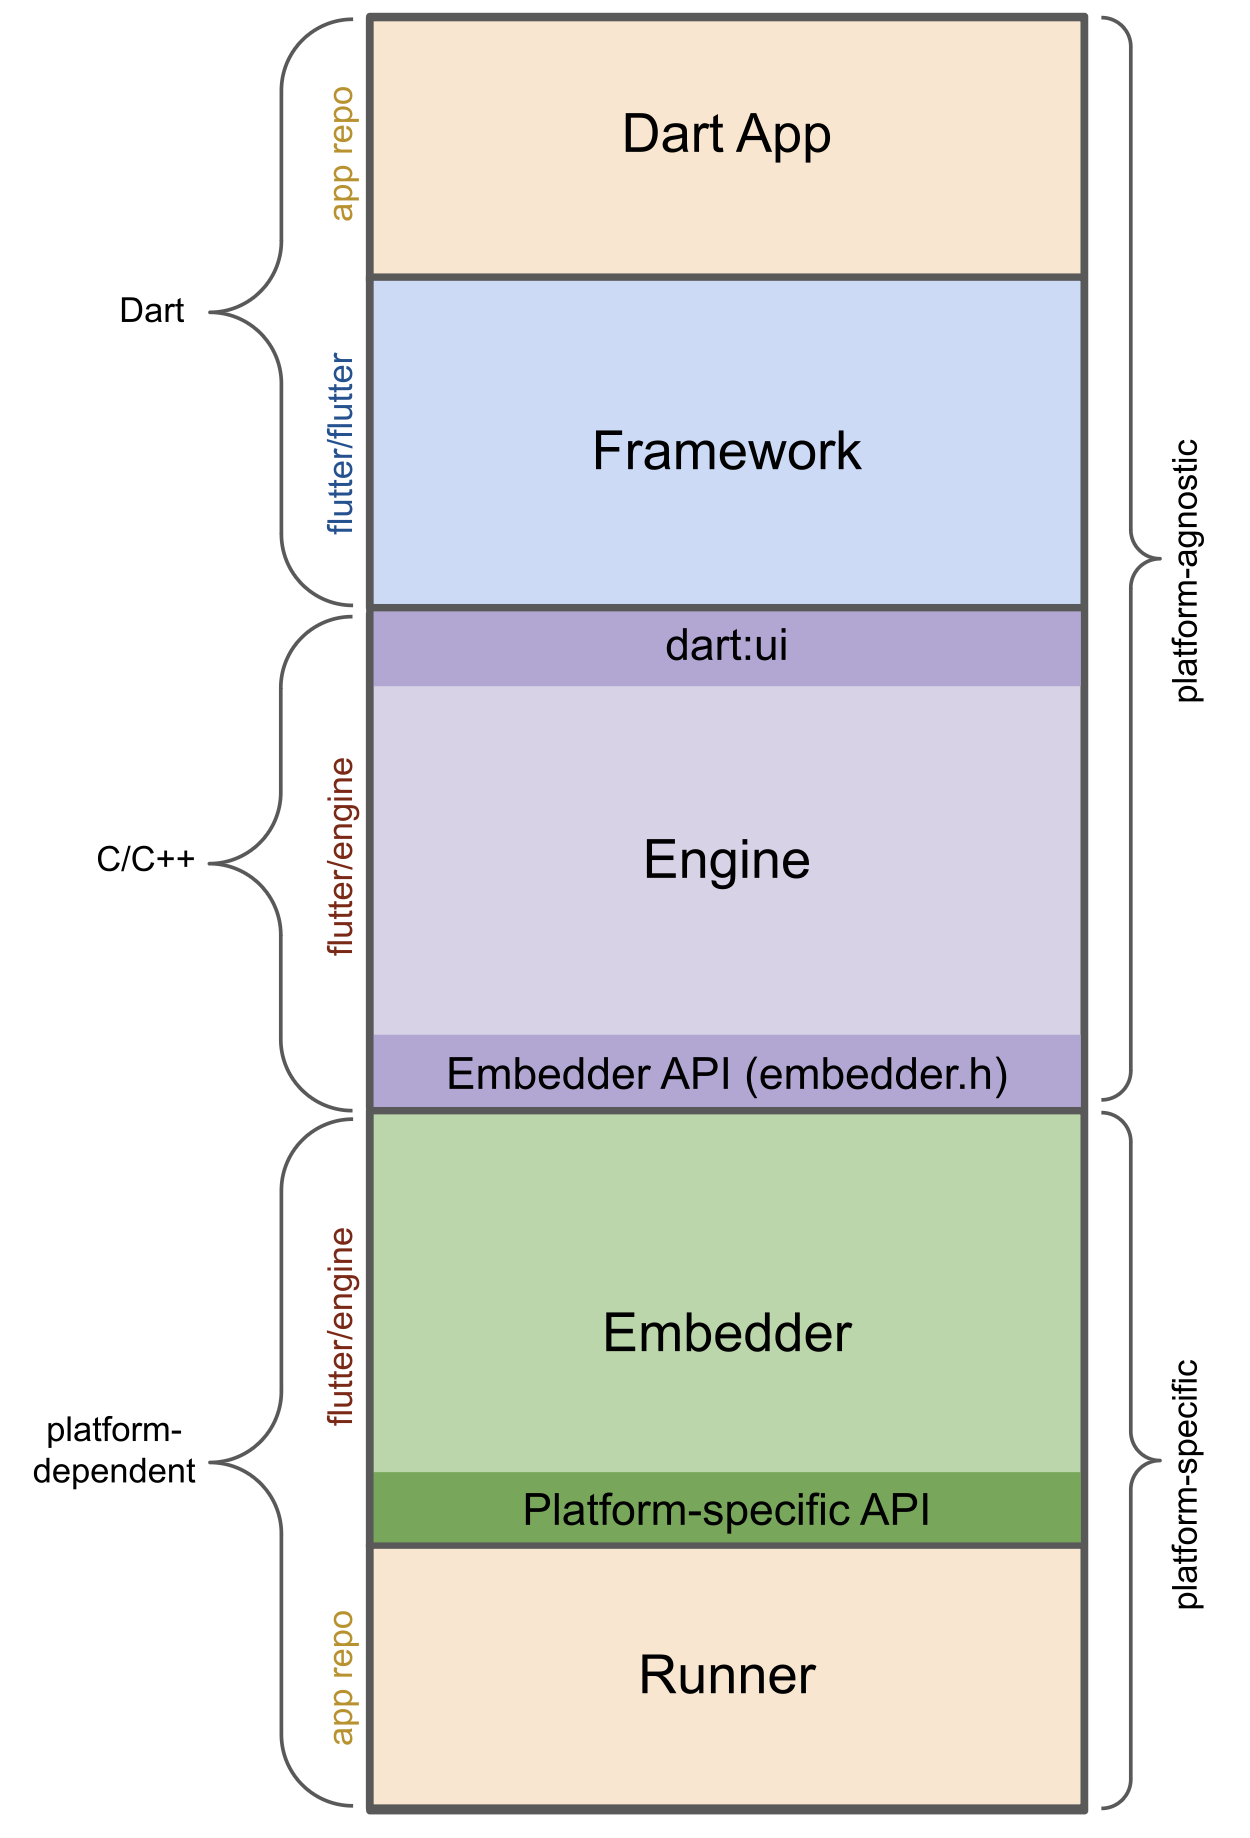
\includegraphics[width=0.4\columnwidth]{images/flutter-app-anatomy.png} 
    \caption{Struttura di un'applicazione in \emph{Flutter}.}
    \label{fig:architettura-flutter}
\end{figure}

Lo stato posseduto dai \lstinline{StatefulWidget} (vedi sezione \ref{subsec:flutter}) può essere considerato come \emph{ephemeral} (ing. effimero) o \emph{app state} (ing. stato dell'applicazione). \\
\emph{Ephemeral} è uno stato che può essere opportunamente confinato all'interno di un singolo \emph{widget} e gestito attraverso la primitiva \lstinline{setState()}, che permette di definire come aggiornarlo.\\
Mentre \emph{app state} è uno stato che viene condiviso tra più \emph{widget} e per la sua gestione, più complessa utilizzando solamente la primitiva sopra citata, esistono diverse librerie di terze parti, ciascuna con le proprie peculiarità a seconda del caso d'uso.\\
\indent La problematica di come gestire lo stato dell'applicazione è definito in gergo \emph{state management}\cite{site:flutter-state-mgmt}, e dopo un'attenta analisi delle librerie disponibili, si è scelto di utilizzare \emph{Riverpod}\cite{site:riverpod}.\\

\subsection{Riverpod}
\label{subsec:riverpod}
% cos'è
% come funziona
% vantaggi
% svantaggi
% motivazione della scelta
\emph{Riverpod} semplifica notevolmente lo \emph{state management} e si basa su un concetto evoluto da \emph{Provider}\cite{site:provider}, libreria da cui deriva.\\
A differenza di \lstinline{InheritedWidget}\cite{site:inheritw} che permette di condividere lo stato tra più \emph{widget}, \emph{Riverpod}, che ne è una reimplementazione, fornisce \emph{providers} che sono indipendenti dai \emph{widget}, in quanto una volta dichiarato il \lstinline{ProviderScope} a livello globale, possono essere richiamati ovunque.\\
Da questo ne consegue che si evita di aggiornare l'interfaccia grafica, ovvero di richiamare il metodo \lstinline{build()} di un \emph{widget} quando non è necessario, poichè è un'operazione costosa.
Un \emph{provider} dunque è un oggetto che può essere richiamato da un \emph{widget} con la finalità di leggerne un valore.\\
Ne esistono di varie tipologie, per le quali si rimanda alla documentazione ufficiale\cite{site:riverpod}, ma quelle utilizzate in questo progetto sono:
\begin{itemize}
    \item \lstinline{FutureProvider}: utilizzato per ricevere un valore generato da un'operazione asincrona (es: richiesta \gls{httpg}\glsoccur);
    \item \lstinline{StateNotifierProvider}: utilizzato per gestire una classe che mantiene uno stato, più complesso di una semplice variabile primitiva, e di esporre dei metodi per monitorarlo o aggiornarlo.
\end{itemize}

\subsection{Architettura dell'applicazione}
\label{subsec:architettura-app}

Per l'architettura dell'applicazione si è scelto di utilizzare un \emph{pattern} architetturale basato su \gls{mvcg}\glsoccur, che permette di separare la logica dell'applicazione dalla sua rappresentazione grafica, in modo da rendere più semplice la manutenzione e l'aggiunta di nuove funzionalità.\\
Nel dettaglio l'applicazione è composta da quattro livelli:
\begin{itemize}
    \item \textbf{Data Layer}: contiene le classi che si occupano di recuperare i dati dal server, attraverso richieste \gls{httpg}\glsoccur, e di convertirli in oggetti rappresentati nel \emph{domain layer};
    \item \textbf{Domain Layer}: contiene le classi che rappresentano i dati dell'applicazione;
    \item \textbf{Application Layer}: contiene le classi che si occupano di gestire la logica dell'applicazione;
    \item \textbf{Presentation Layer}: contiene le classi che si occupano di gestire l'interfaccia, ovvero di eseguire il rendering dei \emph{widget} e di gestire gli eventi generati dall'utente.
\end{itemize}
Questa architettura permette inoltre di avere la possibilità di definire eventualmente più sorgenti da cui recuperare i dati senza dover modificare il codice relativo ai livelli superiori, in quanto è sufficiente modificare il \emph{data layer}\cite{site:app-architecture}.\\

\section{Struttura del progetto}
\label{sec:struttura-progetto}
% Struttura del progetto: cartelle, file, ecc. -> LAYER FIRST
Un altro aspettato importante da considerare per la realizzazione di un progetto software è la sua struttura, ovvero come organizzare i file e le cartelle che lo compongono.\\
Dopo opportune ricerche ed analisi, si è scelto di adottare, tra le due alternative disponibili, la struttura \emph{layer first}, che prevede di organizzare i file e le cartelle in base al livello a cui appartengono, in modo da rendere più semplice la manutenzione e l'aggiunta di nuove funzionalità.\\
\emph{Feature first}, l'altra alternativa, organizza invece i file e le cartelle, mantendendo la separazione tra i livelli, in base alle funzionalità che l'applicazione offre.\\
Il motivo principale per cui la scelta non è ricaduta su quest'ultima è che, nonostante sia quella che garantisca un'organizzazione e manutenzione del codice migliore, risulta essere più complessa da implementare in quanto adatta per progetti di dimensione e complessità maggiore.\\
Di seguito verranno illustrati entrambi gli approcci, in modo da poterli confrontare e comprendere meglio le loro differenze\cite{site:project-structure}.\\
\begin{multicols}{2}
    \begin{verbatim}
        // LAYER FIRST
        lib/
            data/
                feature1.dart
                feature2.dart
            domain/
                feature1.dart
                feature2.dart
            application/
                feature1.dart
                feature2.dart
            presentation/
                feature1.dart
                feature2.dart
    \end{verbatim}
    \begin{verbatim}
        // FEATURE FIRST
        lib/
            feature1/
                data.dart
                domain.dart
                application.dart
                presentation.dart
            feature2/
                data.dart
                domain.dart
                application.dart
                presentation.dart
    \end{verbatim}
\end{multicols}

% \section{Diagrammi UML}
% \label{sec:uml}
% dove inserirli?
% UML -> Diagrammi delle classi

% \subsubsection{Namespace 1} %**************************
% Descrizione namespace 1.

% \begin{namespacedesc}
%     \classdesc{Classe 1}{Descrizione classe 1}
%     \classdesc{Classe 2}{Descrizione classe 2}
% \end{namespacedesc}

\section{Ambiente di sviluppo}
\label{sec:ambiente-sviluppo}
% SEGUI ISSUE #4 E #5 PER LA STESURA DI QUESTA SEZIONE
Di seguito viene descritto l'ambiente di sviluppo e data una panoramica delle tecnologie e strumenti utilizzati.

\subsection*{Figma}
\label{subsec:figma}

\emph{Figma}\cite{site:figma} è un software di editor di grafica vettoriale che permette di progettare interfacce grafiche per applicazioni \emph{web} e \emph{mobile}.\\
È stato utilizzato per la realizzazione del \gls{mockup}\glsoccur dell'applicazione, in quanto vi è la possibilità di creare un prototipo interattivo, che simula l'interazione dell'utente con l'applicazione, e di condividerlo con il team di sviluppo, in modo da avere un'idea più chiara di come l'applicazione debba essere strutturata e di come debba funzionare.\\

\subsection*{Git}
\label{subsec:git}

\emph{Git}\cite{site:git} è un sistema di controllo di versione, finalizzato al tracciamento del codice sorgente e delle sue modifiche, inoltre ne permette la condivisione e dunque la collaborazione tra più sviluppatori.\\
Inoltre è possibile, eventualmente, in caso di errori, di poter ripristinare una versione precedente del codice sorgente.\\

\subsection*{GitHub}
\label{subsec:github}

% DA DEFINIRE: ISSUE, MILESTONE
\emph{GitHub}\cite{site:github} è un servizio di hosting per il codice sorgente di progetti software che utilizza \emph{Git}.\\
Per questo progetto è stato utilizzato per la condivisione e gestione del codice sorgente attraverso una repository dedicata, fornita dall'azienda.\\
Per la pianificazione della fase di implementazione è stato utilizzato il sistema di \gls{issuetracking}\glsoccur integrato, creando delle \gls{milestone}\glsoccur per ogni classe di obbiettivi da raggiungere in base alla loro priorità (vedi sezione \ref{sec:obiettivi}).\\
In ciascuna \gls{milestone}\glsoccur sono state create delle \emph{issue}, in base ai requisiti o ad un insieme di questi, necessarie per il raggiungimento di ciascun obbiettivo, garantendo così una maggiore organizzazione e tracciabilità del lavoro svolto e dei progressi fatti.\\

\subsection*{VSCode}
\label{subsec:vscode}

Editor di codice sorgente \gls{open-source}\glsoccur che oltre a fornire le funzionalità di base necessarie per lo sviluppo (ad esempio: controllo di sintassi, \emph{debugging}, analisi statica del codice, ecc.), supporta molti linguaggi di programmazione ed è possibile estendere le sue funzionalità o il numero di linguaggi supportati attraverso delle estensioni.\\
Di fatto per questo progetto si è reso necessario l'installazione di alcune estensioni, tra cui:
\begin{itemize}
    \item \textbf{Flutter}\cite{site:flutter-extension};
    \item \textbf{Dart}\cite{site:dart-extension}.
\end{itemize}

\subsection*{Flutter}
\label{subsec:flutter}

\emph{Flutter}\cite{site:flutter} è un \gls{framework}\glsoccur che consente di sviluppare applicazioni native per diverse piattaforme, come Android, iOS, web e desktop, utilizzando un unico linguaggio di programmazione, riducendo i tempi e i costi di produzione, senza compromettere le prestazioni dell'applicazione.\\
Il concetto centrale di \emph{Flutter} è quello dei \emph{widget}, oggetti che descrivono come deve essere visualizzata una parte dell'interfaccia grafica. Questi possono essere di due tipi:
\begin{itemize}
    \item \textbf{StatelessWidget}: non hanno uno stato interno, ovvero non cambiano nel tempo, e sono definiti da un insieme di proprietà, chiamate \emph{proprietà immutabili}, che vengono passate al costruttore del \emph{widget};
    \item \textbf{StatefulWidget}: al contrario, possiedono uno stato interno mutabile, e viene usato quando una parte dell'interfaccia utente può cambiare dinamicamente.
\end{itemize}

\subsection*{StarUML}
\label{subsec:staruml}

\emph{StarUML}\cite{site:staruml} è uno strumento di modellazione per sistemi software che sono sviluppati secondo il paradigma \emph{orientato agli oggetti}, attraverso la creazione di diagrammi \gls{umlg}\glsoccur.\\
È stato utilizzato per la realizzazione dei casi d'uso (vedi sezione \ref{sec:usecase}) e dei diagrammi delle classi.\\

\subsection*{Emulatori Android e iOS}
\label{subsec:emulatori}

Per testare l'applicazione su dispositivi \emph{Android} e \emph{iOS} è stato utilizzato rispettivamente \emph{Android Studio}\cite{site:android-studio} e \emph{Xcode}\cite{site:xcode}, che forniscono degli emulatori per le rispettive piattaforme.\\

A completare l'ambiente di sviluppo, l'azienda mi ha fornito l'accesso alle \gls{apig}\glsoccur del loro \gls{backend}\glsoccur attraverso lo \emph{Swagger}\cite{site:swagger}, strumento che, tra le altre cose, consente di consultare la documentazione delle \gls{apig}\glsoccur e di testarle attraverso un'interfaccia grafica \emph{web}.\\
Si specifica che per lo sviluppo dell'applicazione, l'utilizzo di tali \gls{apig} è stato svolto su un \emph{server} di collaudo.
    \chapter{Implementazione}
\label{cap:implementazione}

\intro{In questo capitolo si discuterà dell'implementazione (o codifica) dell'applicazione in conseguenza alle scelte progettuali descritte nel capitolo precedente. Inoltre verranno descritte le librerie di terze parti utilizzate, motivandone la scelta.}\\

Seguendo quanto descritto nel capitolo \ref{cap:progettazione}, si è proceduto con l'implementazione del prodotto software.\\
Di seguito verrà illustratta l'effettiva struttura del progetto basata sull'approccio \emph{layer first} (sezione \ref{sec:struttura-progetto}), descrivendone poi la varie classi contenute nei file di ciascuna cartella. \\

\begin{verbatim}
    assets/
    lib/
        components/
        constants/
        data/
            model/
            service/
        provider/
        screens
        styles/
        utils/
        main.dart
\end{verbatim}

L'architettura menzionata nella sezione \ref{subsec:architettura-app} è stata implementata nel seguente modo: il \emph{data layer} e \emph{domain layer} sono stati implementati rispettivamente in \lstinline{service} e \lstinline{model}, contenute all'interno della cartella \lstinline{data}, mentre l'\emph{application layer} è stato implementato nella cartella \lstinline{provider} e il \emph{presentation layer} nella cartella \lstinline{screens}.\\
Le restanti invece sono servite come ausilio per l'implementazione delle funzionalità dei \emph{layer} sopracitati, come ad esempio \lstinline{components} per la creazione di \emph{widget} personalizzati e utilizzati dal \emph{presentation layer}.

\section{Components}
\label{sec:components}

In questa cartella sono raccolti tutti i \emph{widget} personalizzati, utilizzati dalle schermate presenti in \emph{screens} (sezione \ref{sec:screens}).\\
Di seguito verranno descritti i vari \emph{widget} implementati, suddivisi in base alla loro funzionalità.\\
Si specifica inoltre che la maggior parte di questi abbiano una visibilità pubblica, in quanto devono essere utilizzati dalle schermate, mentre alcuni hanno una visibilità privata, poichè sono stati creati per essere utilizzati esclusivamente all'interno di altri \emph{widget} contenuti nel medesimo file.

\subsection{Alert Dialogs}
\label{subsec:alert-dialogs}

Nel file denominato \lstinline{alert_dialogs.dart} sono stati implementati dei \lstinline{StatelessWidget} che consentono di personalizzare un \emph{alert dialog}.

\subsubsection*{CustomBaseAlertDialog}
\label{subsubsec:custom-base-alert-dialog}

È una classe che implementa un \lstinline{AlertDialog}\cite{site:alert-dialog} e ne definisce l'aspetto base, fissando alcuni elementi, come \lstinline{Text}\cite{site:text} per il titolo, \lstinline{Widget} per l'icona posta sotto il titolo, il suo colore e \gls{padding}\glsoccur.\\
Mentre è possibile scegliere se aggiungere o meno un testo descrittivo e dei pulsanti di conferma e/o annulla, in base al contesto dell'operazione.

\subsubsection*{IconAlertDialog}
\label{subsubsec:icon-alert-dialog}

Classe che implementa \lstinline{CustomBaseAlertDialog} personalizzandolo ulteriormente impostando con dei valori fissi sia il \gls{padding}\glsoccur che la dimensione dell'icona.\\
Attraverso il costruttore è obbligatorio passare il \emph{widget} di tipo \lstinline{IconData}\cite{site:icon-data}, il suo colore e un titolo, mentre è opzionale passare un testo descrittivo, e se aggiungere o meno dei bottoni di conferma e/o annulla.

\subsubsection*{LoadingAlertDialog}
\label{subsubsec:loading-alert-dialog}

Personalizzazione di \lstinline{IconAlertDialog} in cui viene impostata come icona un \lstinline{CircularProgressIndicator}\cite{site:circular-progress-indicator}, che rappresenta un indicatore di caricamento.\\
È possibile decidere, attraveso il costruttore, il colore dell'indicatore e il titolo da visualizzare.\\
Lo scopo di questa classe è quella di essere utilizzata per mostrare un indicatore di caricamento durante l'esecuzione di un'operazione asincrona.

\subsubsection*{WarningAlertDialog}
\label{subsubsec:warning-alert-dialog}

Personalizzazione di \lstinline{IconAlertDialog} dove si richiede, nel costruttore, di passare un'icona e il suo colore, un titolo, il contenuto del testo descrittivo, l'azione che deve compiere il bottone di conferma alla sua pressione e il suo stile grafico (sezione \ref{subsec:button-styles}), mentre il pulsante di annullamento è stato fissato.\\
Lo scopo di questa classe è quella di essere utilizzata per mostrare un messaggio di avvertimento all'utente riguardante una scelta e la sua conferma.

\begin{figure}[!h] 
    \centering 
    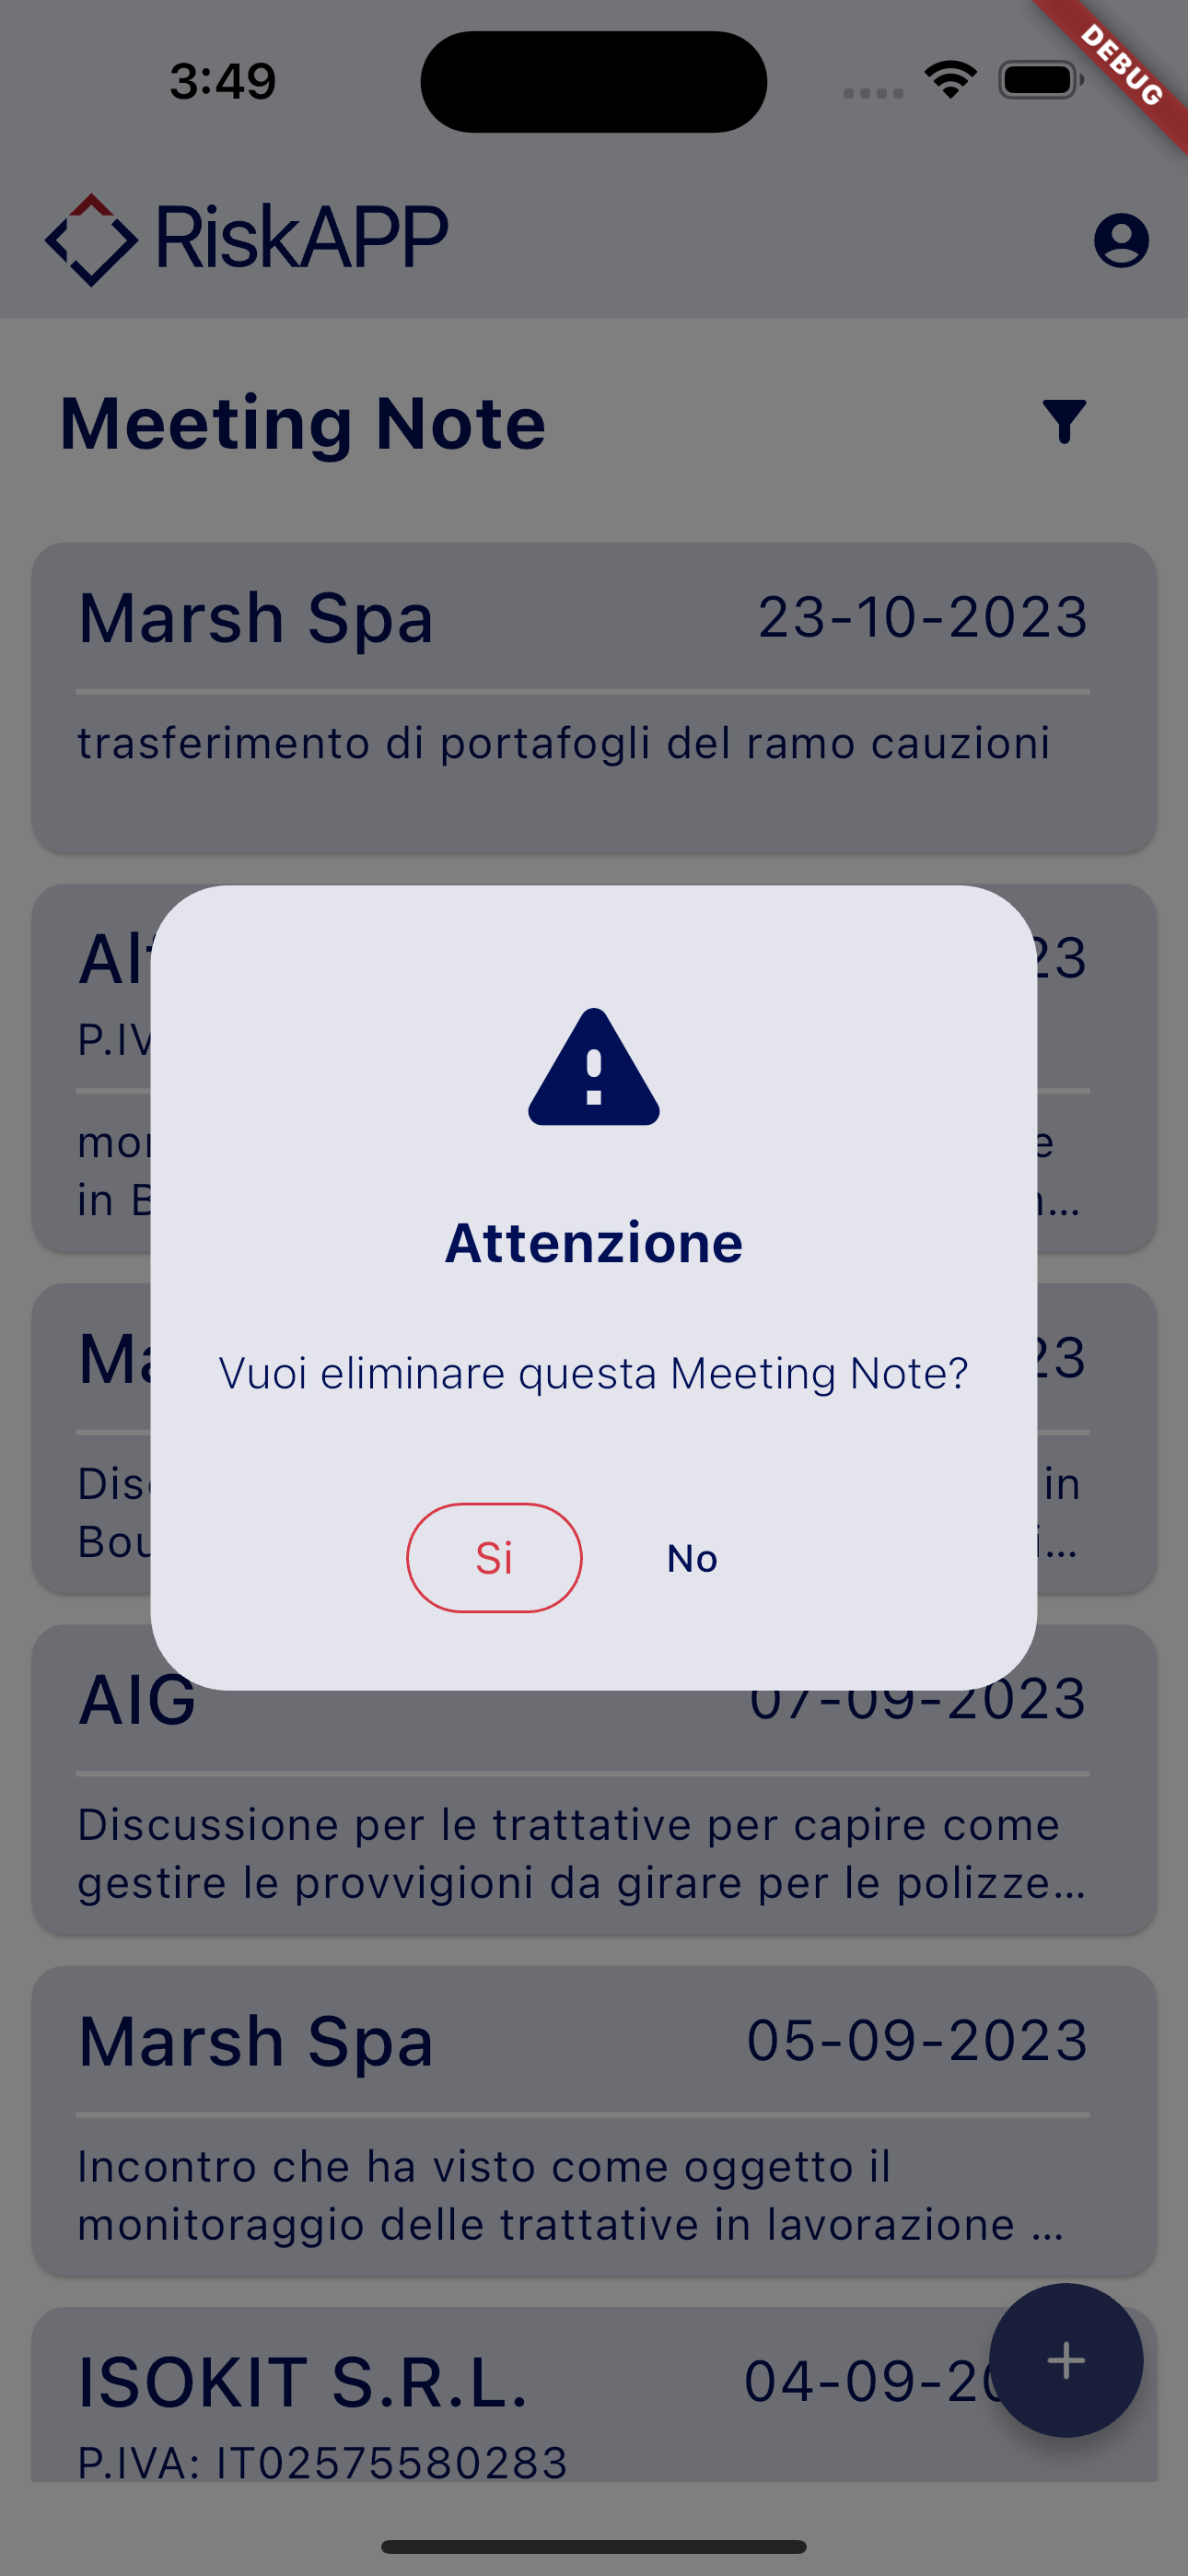
\includegraphics[width=0.3\columnwidth]{screenshot/14-del_dialog} 
    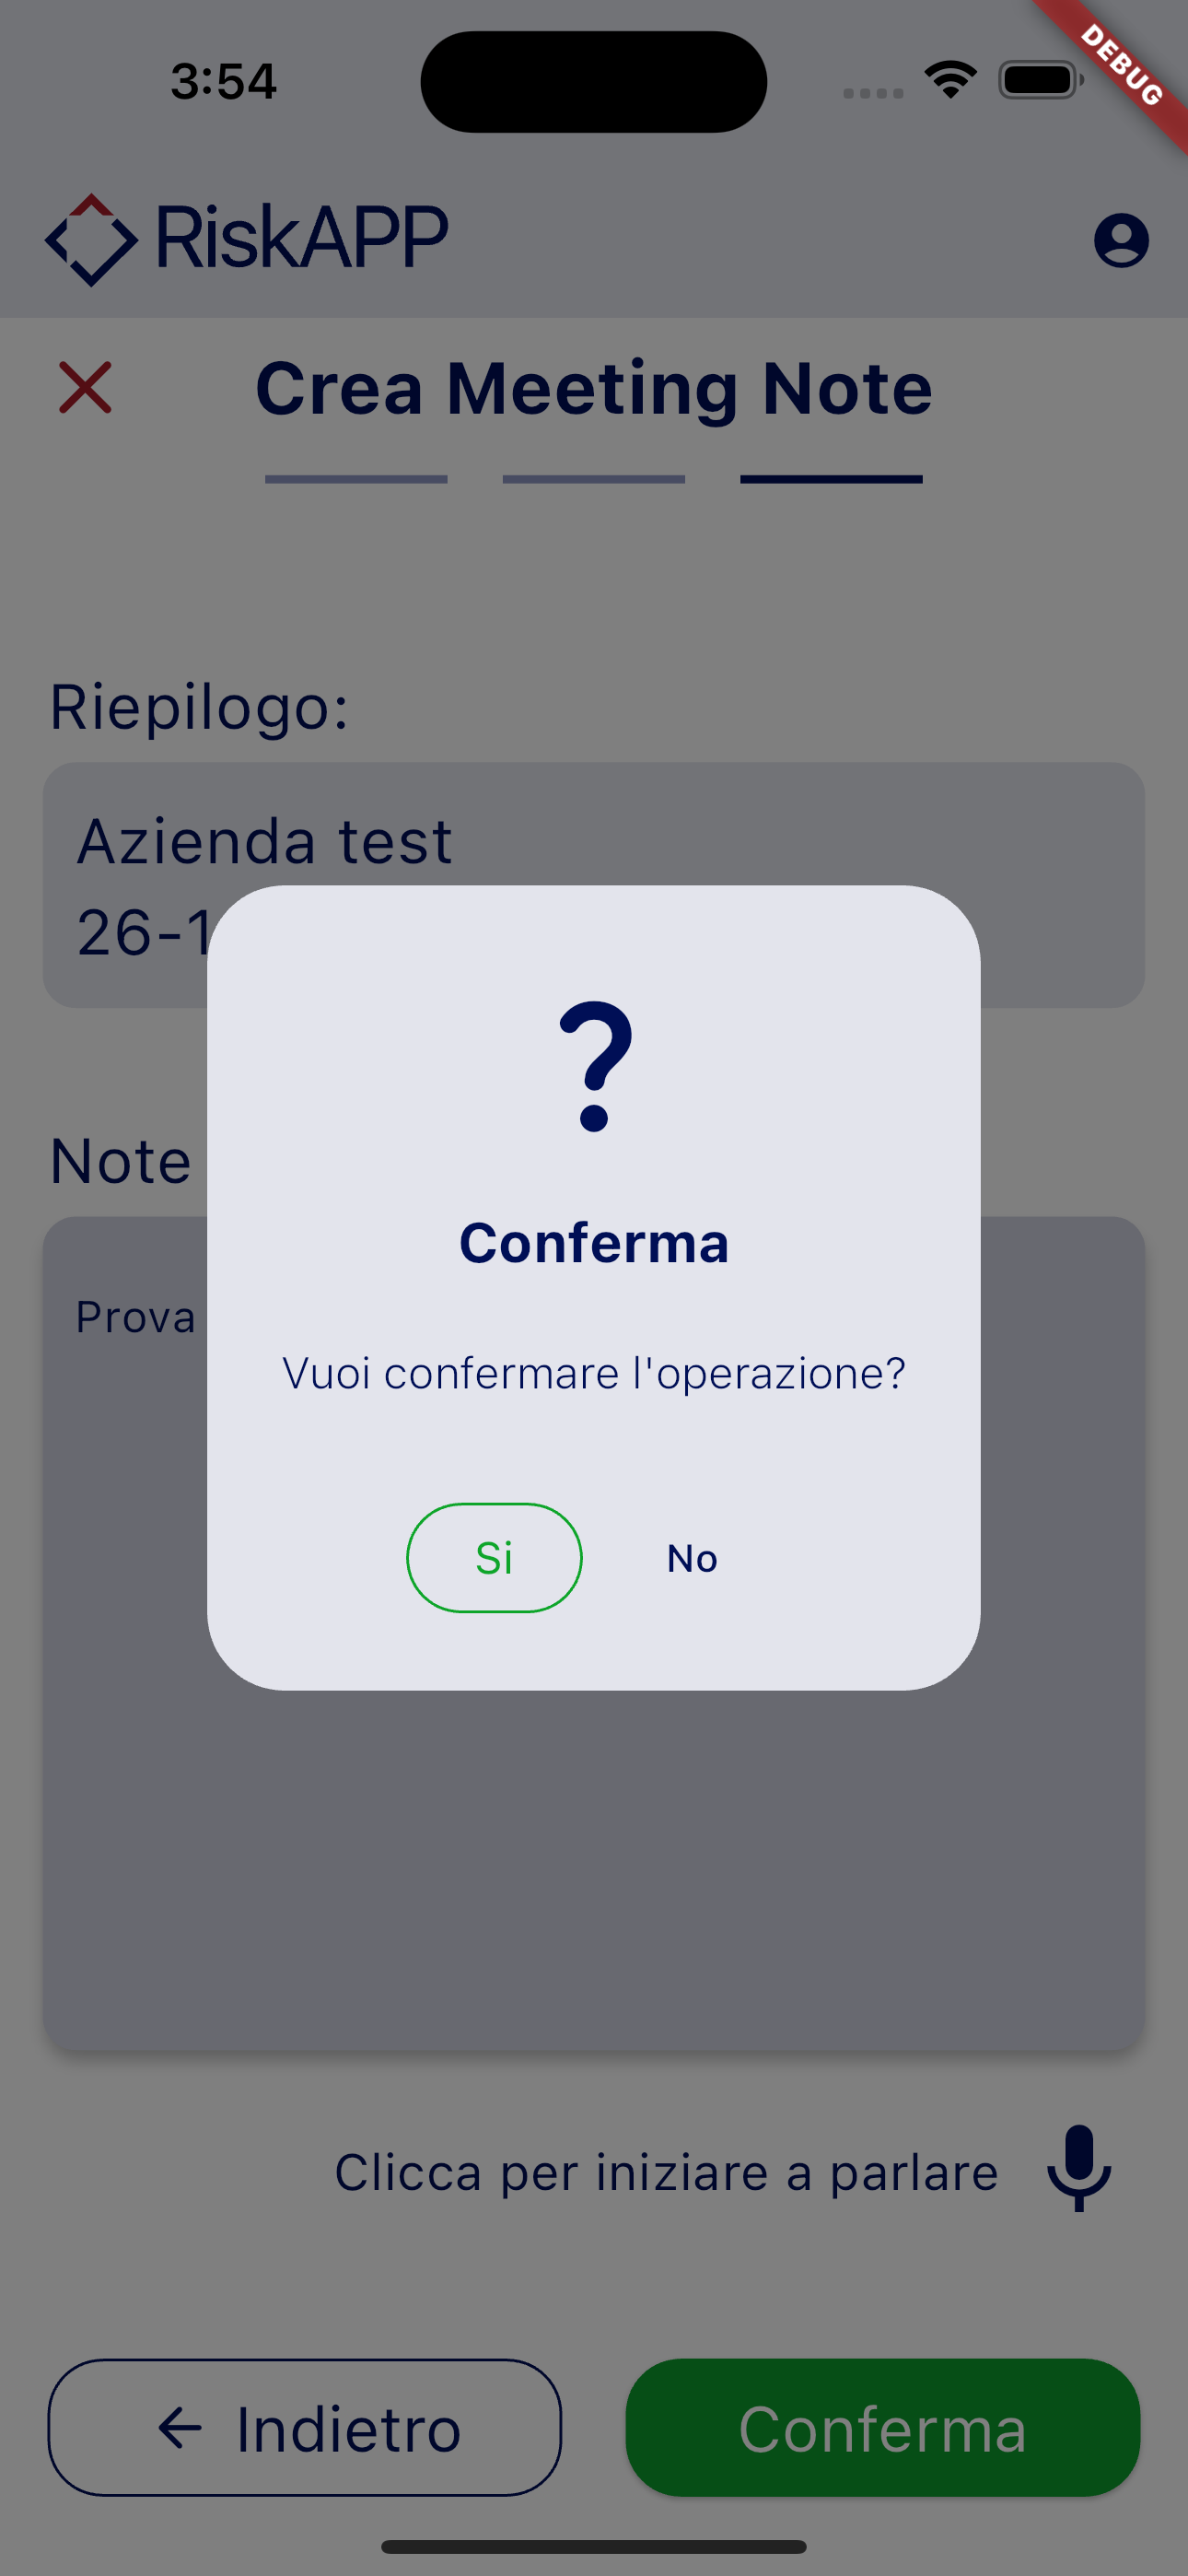
\includegraphics[width=0.3\columnwidth]{screenshot/23-wc3_confirm_dialog}
    \caption{Esempi di \lstinline{WarningAlertDialog}}
    \label{fig:warning-alert-dialog}
\end{figure}

\newpage

\subsubsection*{ResponseDialog}
\label{subsubsec:response-dialog}

Personalizzazione di \lstinline{IconAlertDialog} dove si richiede, nel costruttore, di passare un'icona, il suo colore e un titolo (figura \ref{fig:response-dialog}).\\
Lo scopo di questa classe è quella di essere utilizzata per mostrare un messaggio di risposta all'utente riguardante l'esito di un'operazione.\\

\begin{figure}[!h] 
    \centering 
    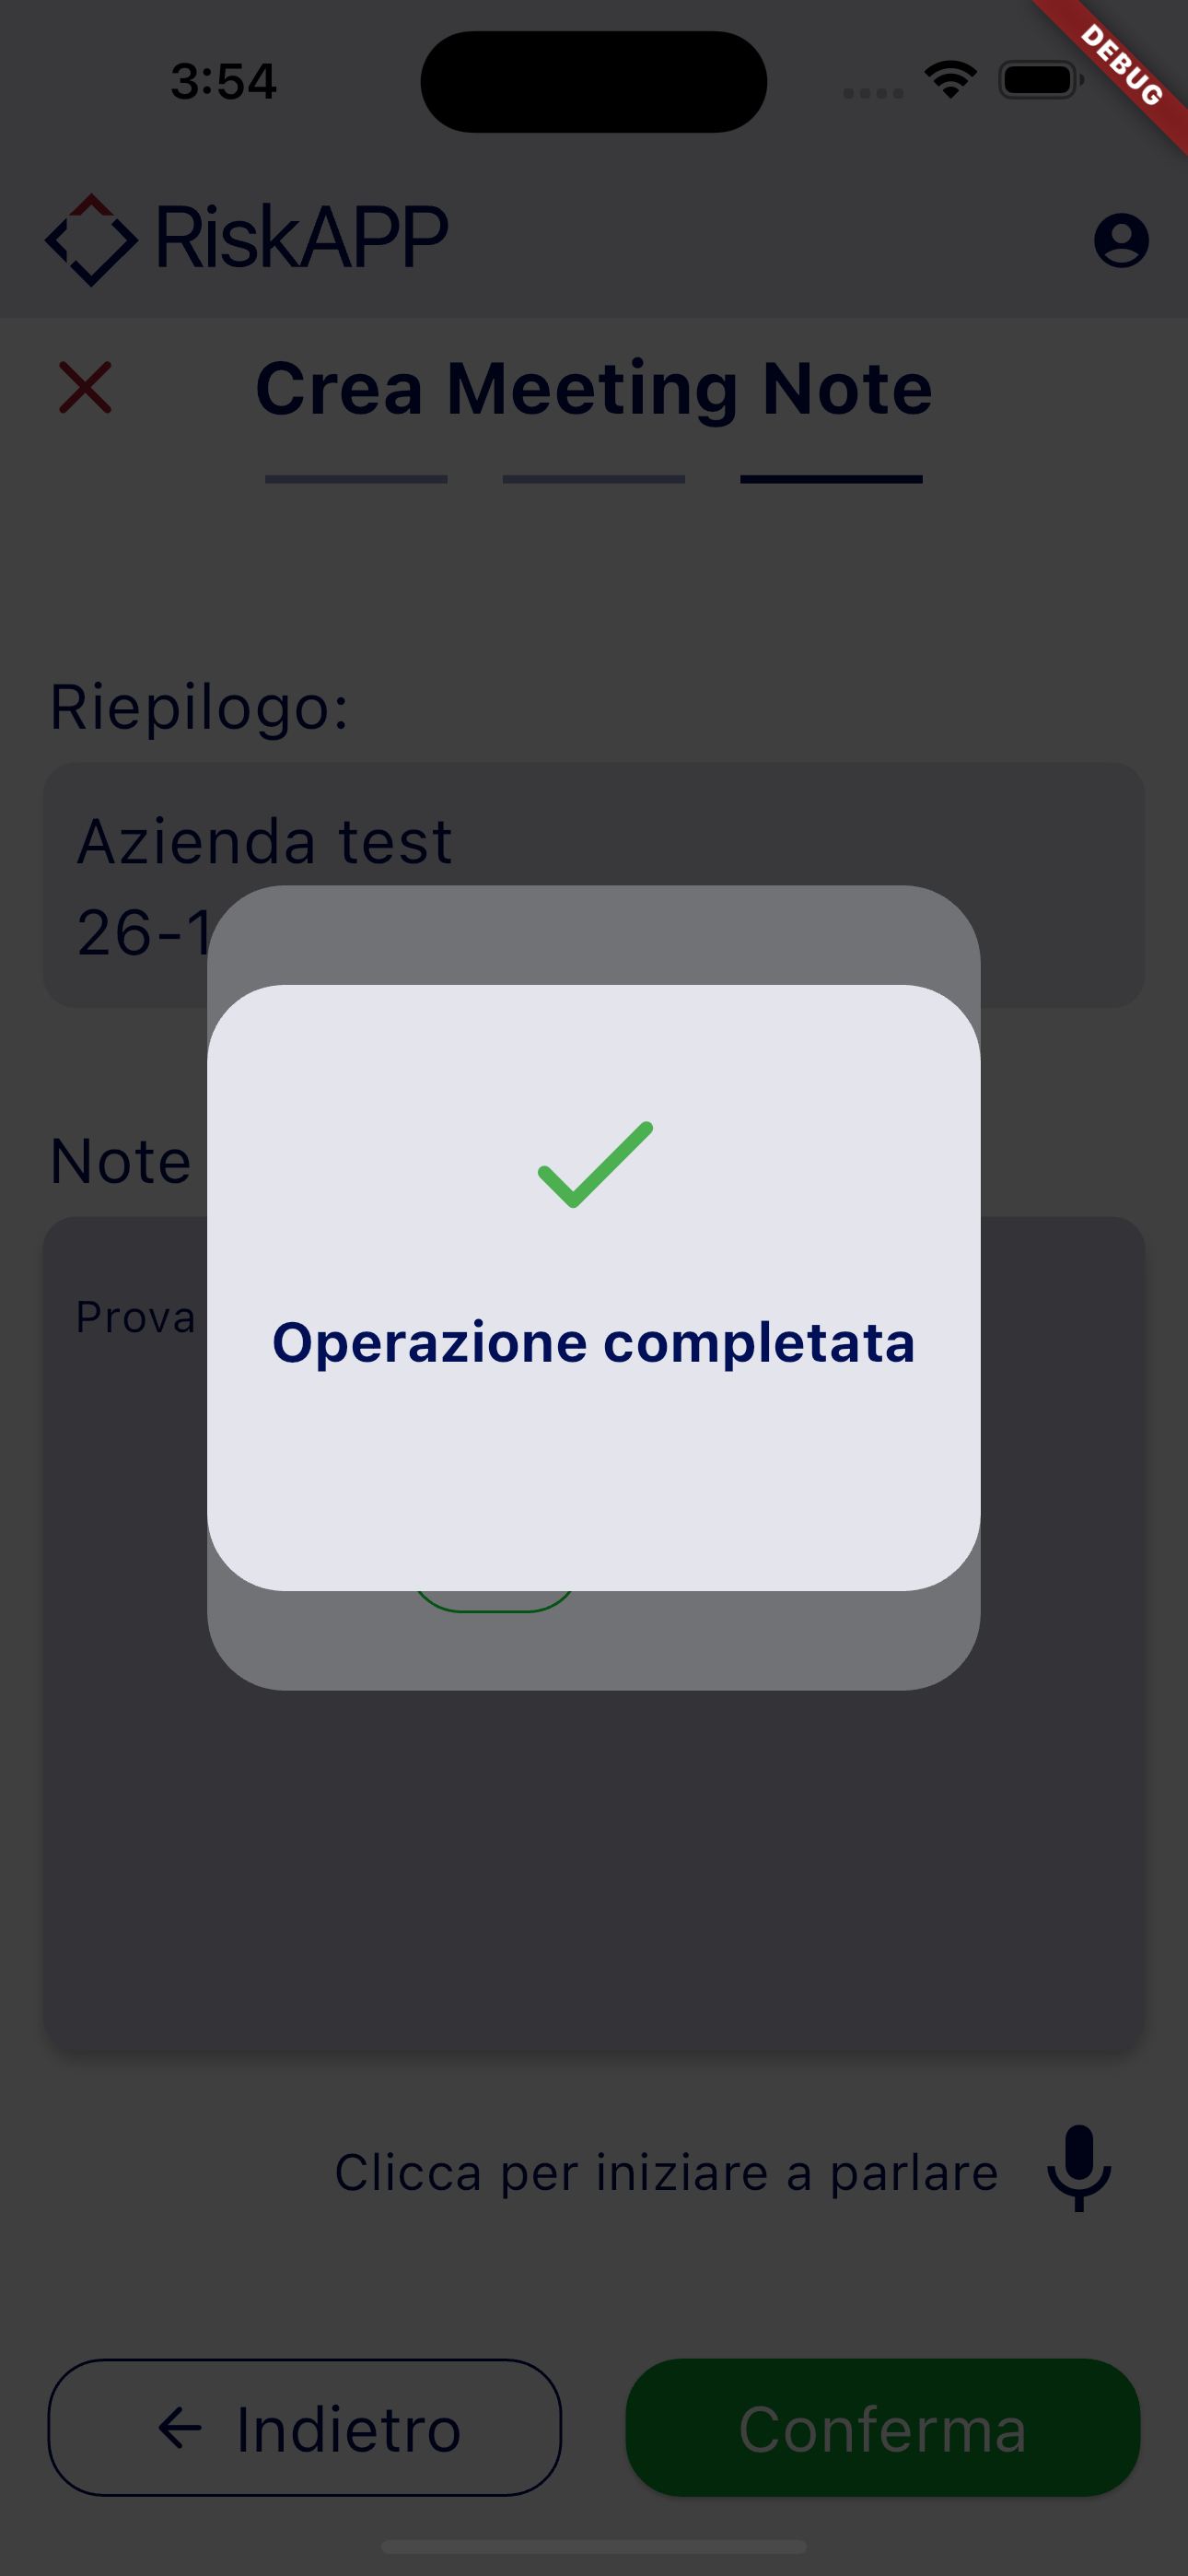
\includegraphics[width=0.3\columnwidth]{screenshot/24-wc3_success_dialog} 
    \caption{Esempio di \lstinline{ResponseDialog}}
    \label{fig:response-dialog}
\end{figure}

\subsection{App Bars}
\label{subsec:app-bars}

Nel file denominato \lstinline{app_bars.dart} sono stati implementati dei \lstinline{StatelessWidget} che consentono di personalizzare un \emph{app bar}.

\subsubsection*{CustomAppBar}
\label{subsubsec:custom-app-bar}

Classe che implementa \lstinline{AppBar}\cite{site:app-bar} definendone il colore di background, applicato dal tema dell'applicazione (sezione \ref{subsec:app-theme}) e il titolo, in cui si tratta dell'applicazione di un'immagine vettoriale contenuta nella cartella \lstinline{assets} la quale rappresenta il logo dell'azienda.\\
Infine è possibile scegliere se aggiungere o meno un'icona, che rappresenta il pulsante di accesso alla schermata dell'account utente (figure \ref{fig:home-screen} e \ref{fig:account-screen}).\\
La motivazione di quest'ultima scelta è a causa del fatto che questa personalizzazione dell'\lstinline{AppBar} viene utilizzata per la quasi totalità delle viste, anche in quella dell'account utente, dove non si rende necessaria l'icona menzionata precedentemente poichè ci si trova già in tale vista.

\subsubsection*{LoginAppBar}
\label{subsubsec:login-app-bar}

Classe che implementa \lstinline{AppBar}, personalizzandolo appositamente per la schermata di \emph{login} (sezione \ref{subsec:login-screen}), che è simile a quella precedente, differenziandosi per la non presenza dell'icona che funge da pulsante di accesso alla schermata dell'account utente e per l'allineamento centrale del titolo (figura \ref{fig:login-screen}).

\subsection{Biomteric Switch}
\label{subsec:biometric-switch}

Nel file denominato \lstinline{biometric_switch.dart} è stato implementato un \lstinline{StatefulWidget} per costruire un componente in grado di permettere all'utente di abilitare il riconoscimento biometrico. \\
Questo \emph{widget} è composto da un \lstinline{Switch}\cite{site:switch} e un \lstinline{Text}\cite{site:text} che rappresenta il testo descrittivo (figura \ref{fig:account-screen}).\\
Inoltre ne viene definito l'aspetto e il comportamento attraverso la definizione di un \lstinline{State} che estende \lstinline{StatefulWidget} implementando il metodo \lstinline{build} per la costruzione del \emph{widget} e il metodo \lstinline{onChanged} per la gestione dell'evento di cambiamento di stato dello \lstinline{Switch}.\\
Stato che è rappresentato da due variabili di tipo \lstinline{bool}, una che si occupa di gestire l'abilitazione del componente e l'altro che indica se nel dispositivo in cui viene eseguita l'applicazione è supportato il riconoscimento biometrico.\\
La prima tra queste, ad ogni suo cambiamento di stato, viene salvata in locale attraverso una libreria di terze parti (di cui verrà discussa nella sezione \ref{subsec:shared-preferences}) per mantenere in memoria la preferenza dell'utente. \\
Il caso in cui la seconda variabile menzionata precedentemente sia \lstinline{false}, dunque non vi è il supporto per il riconoscimento biometrico, si notifica l'utente di tale mancanza e si disabilita lo \lstinline{Switch}.

\subsection{Date Picker}
\label{subsec:date-picker}

Nel file denominato \lstinline{date_picker.dart} sono stati implementati dei \emph{widget} per costruire dei componenti in grado di permettere all'utente di selezionare una data o un intervallo di date.

\subsubsection*{DateButton}
\label{subsubsec:date-button}

Questo componente estende \lstinline{StatelessWidget} e si occupa di costruire un bottone che visualizza la data, o un intervallo di date, selezionata/e dall'utente.\\
Ha visibilità privata, poichè è stato creato per essere utilizzato esclusivamente all'interno dei \emph{widget} contenuti nello stesso file.\\
È composto da un \lstinline{TextButton}\cite{site:text-button}, in cui viene definito l'aspetto grafico, e un \lstinline{Text} per visualizzare la data o un intervallo di date (figura \ref{fig:filter-panel}), passato attraverso il costruttore, insieme anche al comportamento del pulsante, definito attraverso il metodo \lstinline{onPressed}\cite{site:on-pressed}.

\subsubsection*{CustomDateRangePicker}
\label{subsubsec:custom-date-range-picker}

Questo componente estende \lstinline{StatefulWidget} e si occupa di costruire un \emph{widget} che permette all'utente di selezionare un intervallo di date.\\
È composto da \lstinline{DateButton}, al quale il primo parametro che viene passato è l'intervallo di date da visualizzare, di default o selezionato dall'utente, precedentemente formattato da un metodo privato \lstinline{dateFormatter}: riceve in input la data iniziale e finale dell'intervallo (nel caso in cui si intenda selezionare un singolo giorno è sufficiente impostarne con esso entrambi i cambi) e restituisce una stringa che rappresenta l'intervallo di date formattato opportunamente.\\
Mentre come secondo parametro viene passato un altro metodo privato \lstinline{show} che si occupa di visualizzare il calendario e di consentire all'utente di seleziona un intervallo (figura \ref{fig:date-range-picker}). \\
Inoltre è presente un metodo pubblico \lstinline{onDateRangeSelected} che si occupa di gestire l'evento di selezione dell'intervallo di date, aggiornando lo stato del \emph{widget}. \\
Lo scopo di questo \emph{widget} è quello di fornire la possibilità all'utente di selezionare una singola data o intervallo di date per filtrare la lista di \emph{Meeting Note} e viene impiegato solamente all'interno del \lstinline{FilterPanel} (sezione \ref{subsec:filter-panel}).

\begin{figure}[!h] 
    \centering 
    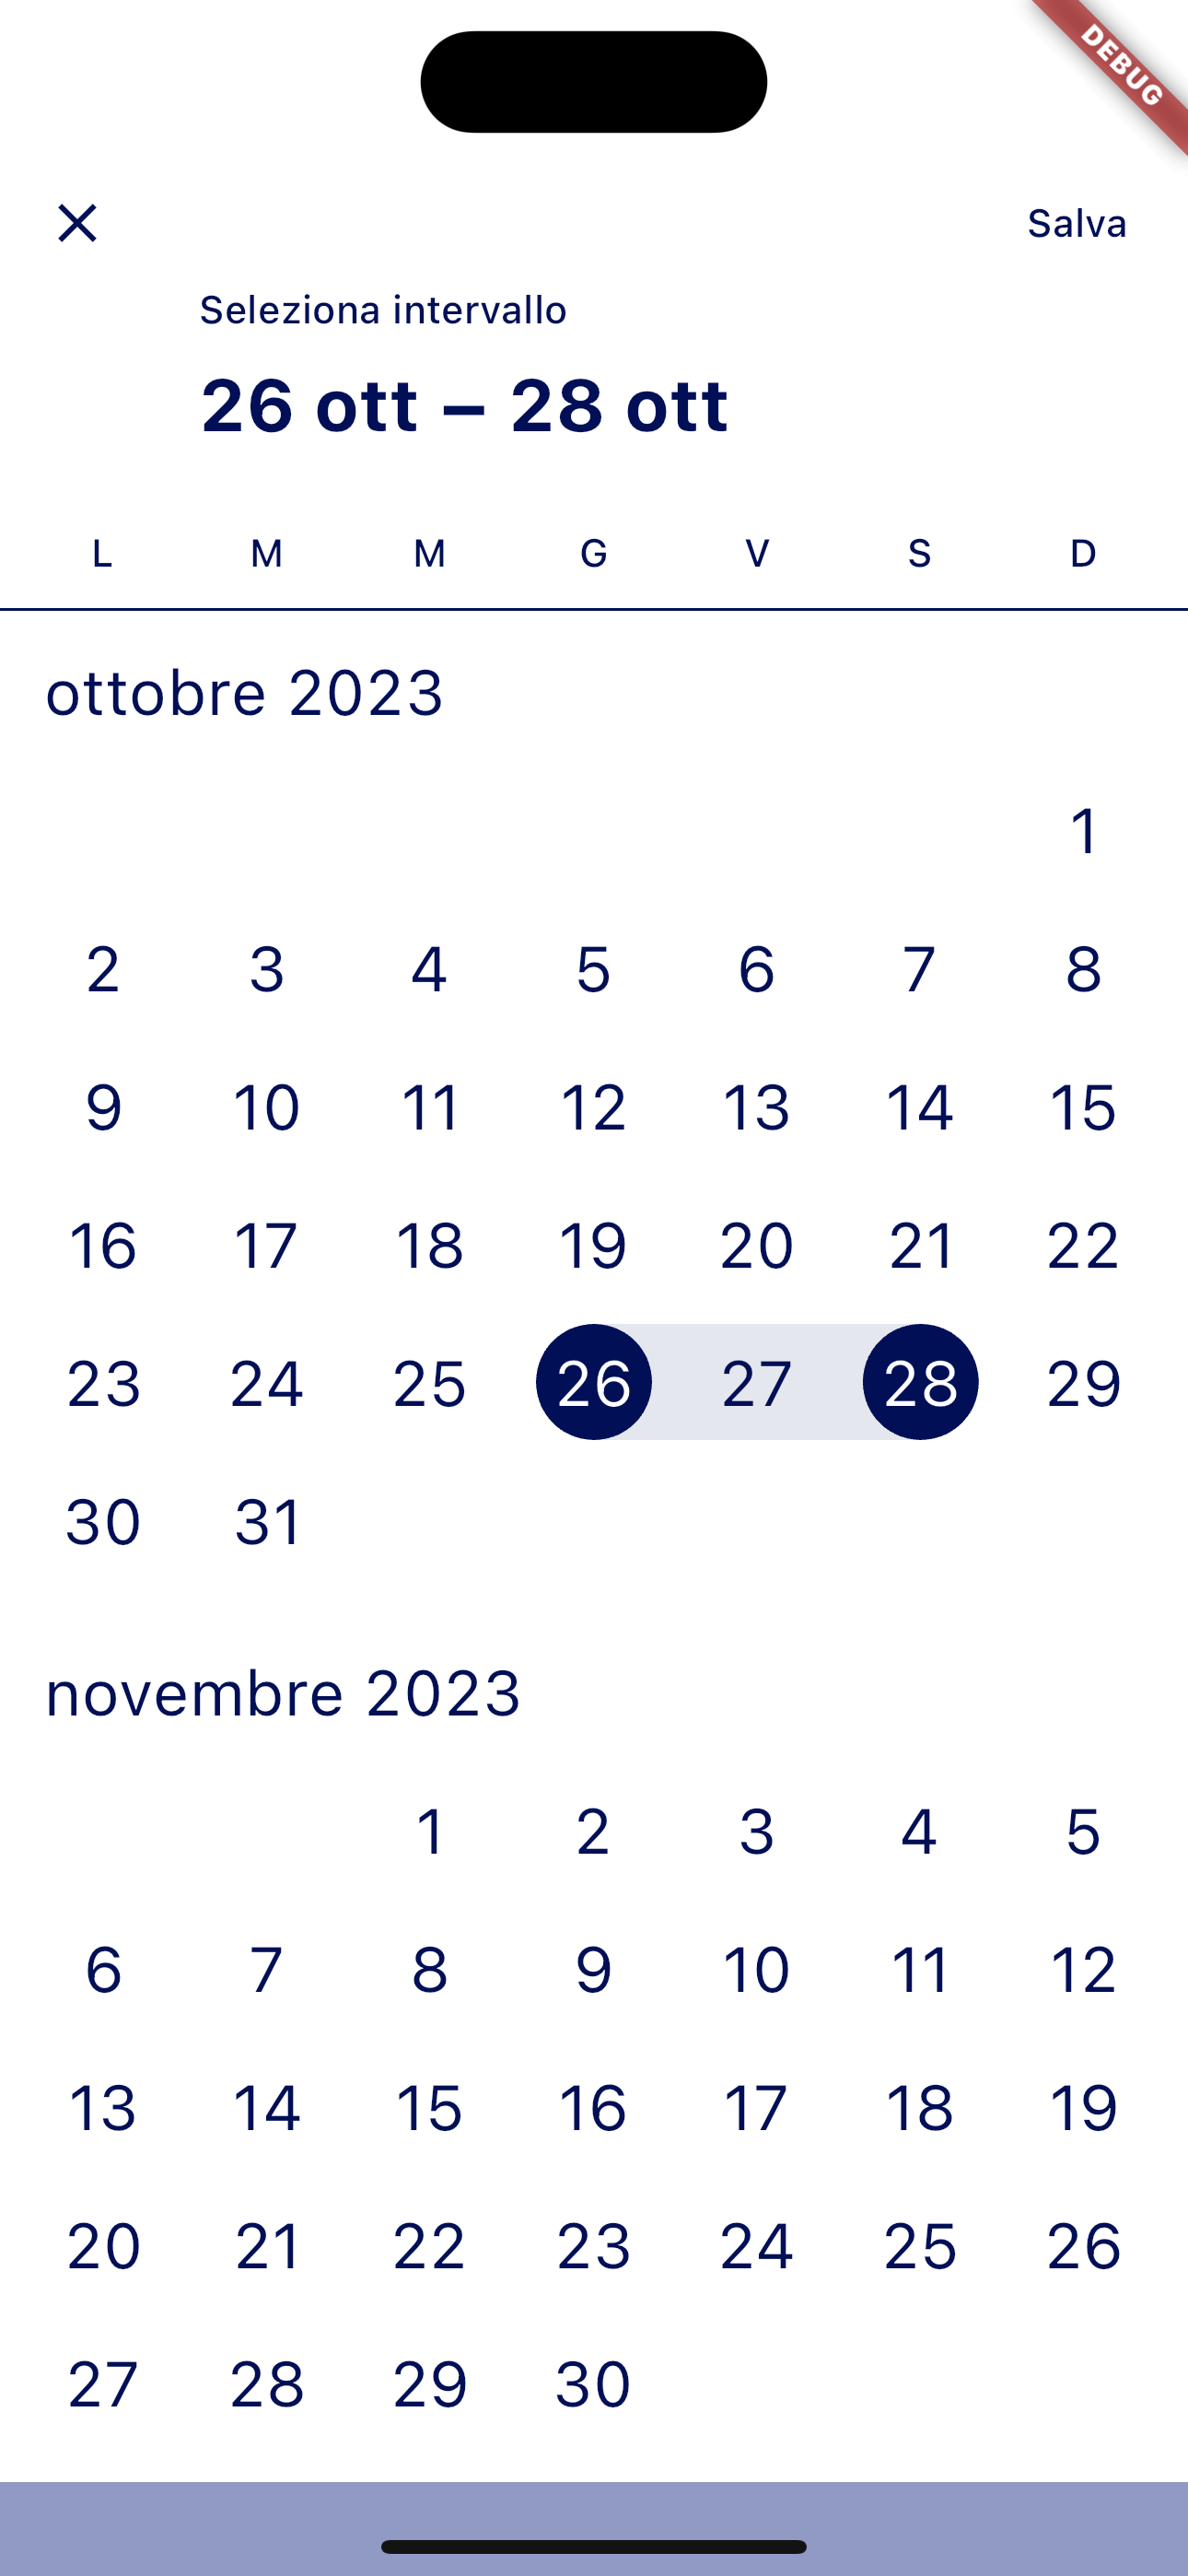
\includegraphics[width=0.3\columnwidth]{screenshot/11-date_range_picker} 
    \caption{Selettore di intervallo di date}
    \label{fig:date-range-picker}
\end{figure}

\subsubsection*{CustomDatePicker}
\label{subsubsec:custom-date-picker}

L'implementazione di questo componente è del tutto analoga a quella di \lstinline{CustomDateRangePicker}, con la differenza che permette all'utente di selezionare una singola data (figura \ref{fig:smart-popup}).\\
Mentre il suo scopo è quello di fornire all'utente, nel momento di revisione dei dati estratti dall'elaborazione del testo da parte di un algoritmo di \emph{intelligenza artificiale}, di modificare la data di una \emph{Meeting Note} da creare.

\subsection{Filter Panel}
\label{subsec:filter-panel}

Nel file denominato \lstinline{filter_panel.dart} è stato implementato un \lstinline{ConsumerStatefulWidget}\cite{site:reading-provider}, il cui comportamento è il medesimo di uno \lstinline{StatefulWidget}, con la differenza che è in grado di leggere i dati forniti da un \emph{Provider} (sezione \ref{subsec:riverpod}).
Tale componente è composto da quattro \emph{widget}, ciascuno dei quali consente di filtrare la lista di \emph{Meeting Note}  secondo i criteri definiti in fase di analisi dei requisiti, che verranno elencati di seguito (figura \ref{fig:filter-panel}):
\begin{itemize}
    \item \lstinline{CustomObjectPicker} (la cui implementazione è discussa nella sezione \ref{subsec:object-picker});
    \item \lstinline{CustomAutocomplete} (la cui implementazione è discussa nella sezione \ref{subsubsec:custom-autocomplete});
    \item \lstinline{CustomDateRangePicker} (la cui implementazione è discussa nella sezione \ref{subsubsec:custom-date-range-picker});
    \item \lstinline{CustomToogleButtons} (la cui implementazione è discussa nella sezione \ref{subsec:toogle-buttons}).
\end{itemize}
Come da prassi, ne viene definito l'aspetto grafico e il comportamento che deve avere.\\
Per quanto riguarda quest'ultimo, che sostanzialmente consiste nel memorizzare e passare alla schermata dedicata quali filtri sono stati attivati dall'utente, tale operazione viene effettuata attraverso uno \lstinline{StateNotifierProvider} (sezione \ref{subsec:riverpod}) e una classe \lstinline{FilteringOptions} (sezione \ref{subsec:filtering}).

\begin{figure}[!h] 
    \centering 
    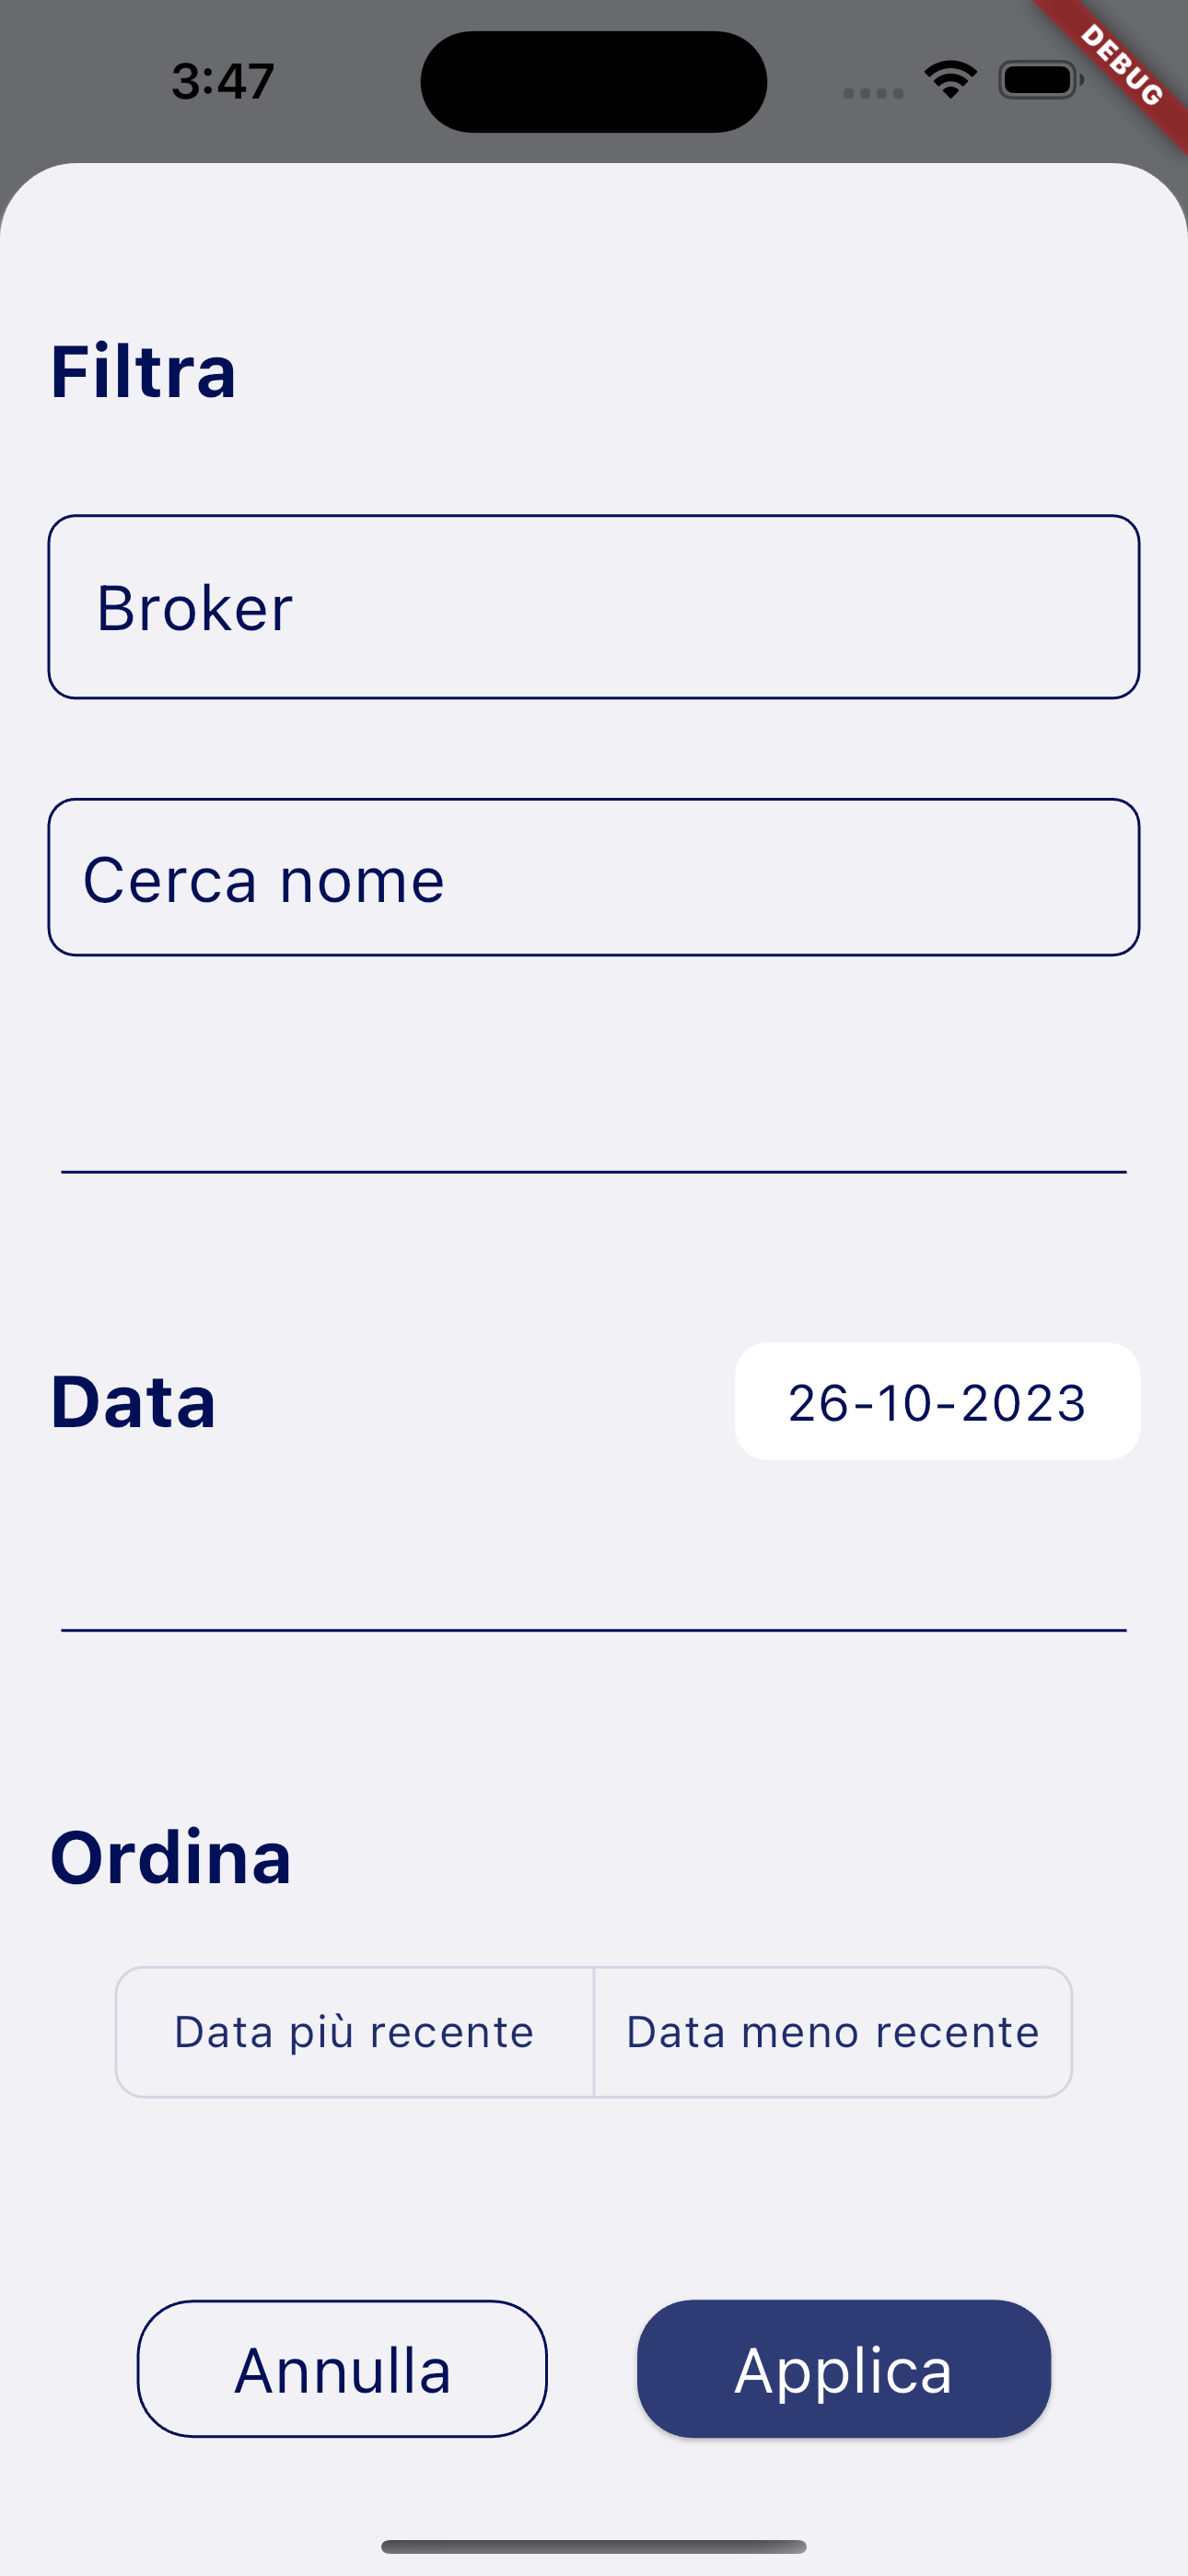
\includegraphics[width=0.3\columnwidth]{screenshot/8-filter_panel} 
    \caption{Popup del \lstinline{FilterPanel}}
    \label{fig:filter-panel}
\end{figure}

\subsection{Login Form}
\label{subsec:login-form}

Nel file denominato \lstinline{login_form.dart} è stato implementato un \lstinline{ConsumerStatefulWidget} (discusso nella sezione \ref{subsec:riverpod}).\\
Lo scopo di questo componente è quello di consentire all'utente di autenticarsi all'applicazione, per farlo ci sono due modi: inserendo manualmente le credenziali oppure utilizzando il riconoscimento biometrico.\\
Per soddisfare il primo caso, il componente è composto da due \lstinline{TextFormField}\cite{site:text-form-field} e un \lstinline{ElevatedButton}\cite{site:elevated-button} di cui vengono definiti l'aspetto grafico.\\
Il \lstinline{TextFormField} riguardante l'inserimento della password presenta anche un pulsante per mostrarla in chiaro o nasconderla (figura \ref{fig:login-screen}).\\
Il pulsante di conferma è disabilitato fintanto che non vengono inserite entrambe le credenziali.\\
Successivamente attraverso l'ausilio di \lstinline{authProvider} (sezione \ref{subsec:authentication-provider}) viene effettuata la richiesta di autenticazione, che in caso di successo porta alla schermata principale dell'applicazione, salvando il \emph{token} di autenticazione ricevuto (sezione \ref{subsec:shared-preferences}), altrimenti viene mostrato un messaggio di errore.\\ 
Mentre nel secondo caso, si effettua un controllo per verificare se l'utente in precedenza aveva abilitato tale funzionalità, in caso affermativo viene eseguito il riconoscimento biometrico (sezione \ref{subsec:biometric-auth}), altrimenti si prosegue con l'inserimento manuale delle credenziali (figura \ref{fig:login-screen}).\\
L'operazione e l'esito dell'autenticazione attraverso il riconoscimento biometrico, che avviene sempre attraverso \lstinline{authProvider}, è simile a quello descritto per l'autenticazione manuale, con la differenza che quest'ultimo metodo preleva le credenziali dalla memoria locale, precedentemente salvate dall'operazione di abilitazione del riconoscimento biometrico da parte dell'utente (sezione \ref{subsec:biometric-switch}). \\
Inoltre è presente una variabile di stato \lstinline{isVerification} che se impostata a \lstinline{true} indica che questa \emph{form} viene impiegata come verifica delle credenziali per confermare l'abilitazione del riconscimento biometrico (sezione \ref{subsec:account-screen}).

\subsection{Meeting Note Card}
\label{subsec:meeting-note-card}

Nel file denominato \lstinline{meeting_note_card.dart} sono stati implementati dei \lstinline{StatelessWidget} per costruire un componente in grado di visualizzare una \emph{Meeting Note} in una lista, e/o in dettaglio, con la possibilità di eliminarla e/o modificarla. \\
Si specifica che tutti i dati necessari da visualizzare sono stati passati attraverso il costruttore.

\subsubsection*{MeetingNoteTitle}
\label{subsubsec:meeting-note-title}

Si tratta di un \emph{widget} che si occupa di disporre gli elementi che compongono il titolo di una 
\emph{Meeting Note}, ovvero l'identificativo del cliente e la data dell'incontro, in modo tale che entrambi siano posizionati sulla stessa riga, con il primo che occupa la maggior parte dello spazio e il secondo che viene posizionato a destra.\\
Inoltre è stato aggiunto un \lstinline{Divider}\cite{site:divider} che funge da separatore tra il titolo e il contenuto parziale della \emph{Meeting Note}, visualizzabile direttamente nella lista di \emph{Meeting Note}.

\subsubsection*{MeetingNoteItem}
\label{subsubsec:meeting-note-item}

\emph{Widget} che effettivamente costruisce l'\emph{item} della lista di \emph{Meeting Note}, composto da un \lstinline{ListTile}\cite{site:list-tile}, in cui nella proprietà \lstinline{title} viene posto \lstinline{MeetingNoteTitle} e in \lstinline{subtitle} il contenuto della \emph{Meeting Note} stroncato ad un massimo di due righe di testo (figura \ref{fig:home-screen}).\\
All'evento \lstinline{onTap} del componente, viene mostrato a schermo una modale che appare dal basso contenente i dettagli della \emph{Meeting Note}.\\
Si vuole precisare che contrariamente a quanto pensato durante la realizzazione del \gls{mockup}\glsoccur, si è deciso di apportare una modifica per quanto riguarda la visualizzazione dei dettagli della \emph{Meeting Note}, in quanto essendo l'applicazione usata da utenti in mobilità, è più ergonomico mostrare i dettagli in una modale che appare dal basso, piuttosto che dall'espansione di un \emph{item}.

\subsubsection*{MeetingNoteCard}
\label{subsubsec:meeting-note-card}

Componente contenuto nella modale menzionata precedentemente, il quale si occupa di disporre tutti gli elementi di cui è composta una \emph{Meeting Note} (figura \ref{fig:meeting-note-card}).\\
È composto da un \lstinline{MeetingNoteTitle}, il contenuto della \emph{Meeting Note}, l'autore e i due pulsanti che permettono di eliminarla e/o modificarla, il comportamento della prima azione viene passata per parametro, mentre per la seconda viene definita direttamente in quanto è stato sufficiente rimandare alla schermata del \emph{wizard} per poi effettuare le modifiche (da sezione \ref{subsec:wizard-screen-1} a \ref{subsec:wizard-screen-3}).

\begin{figure}[!h] 
    \centering 
    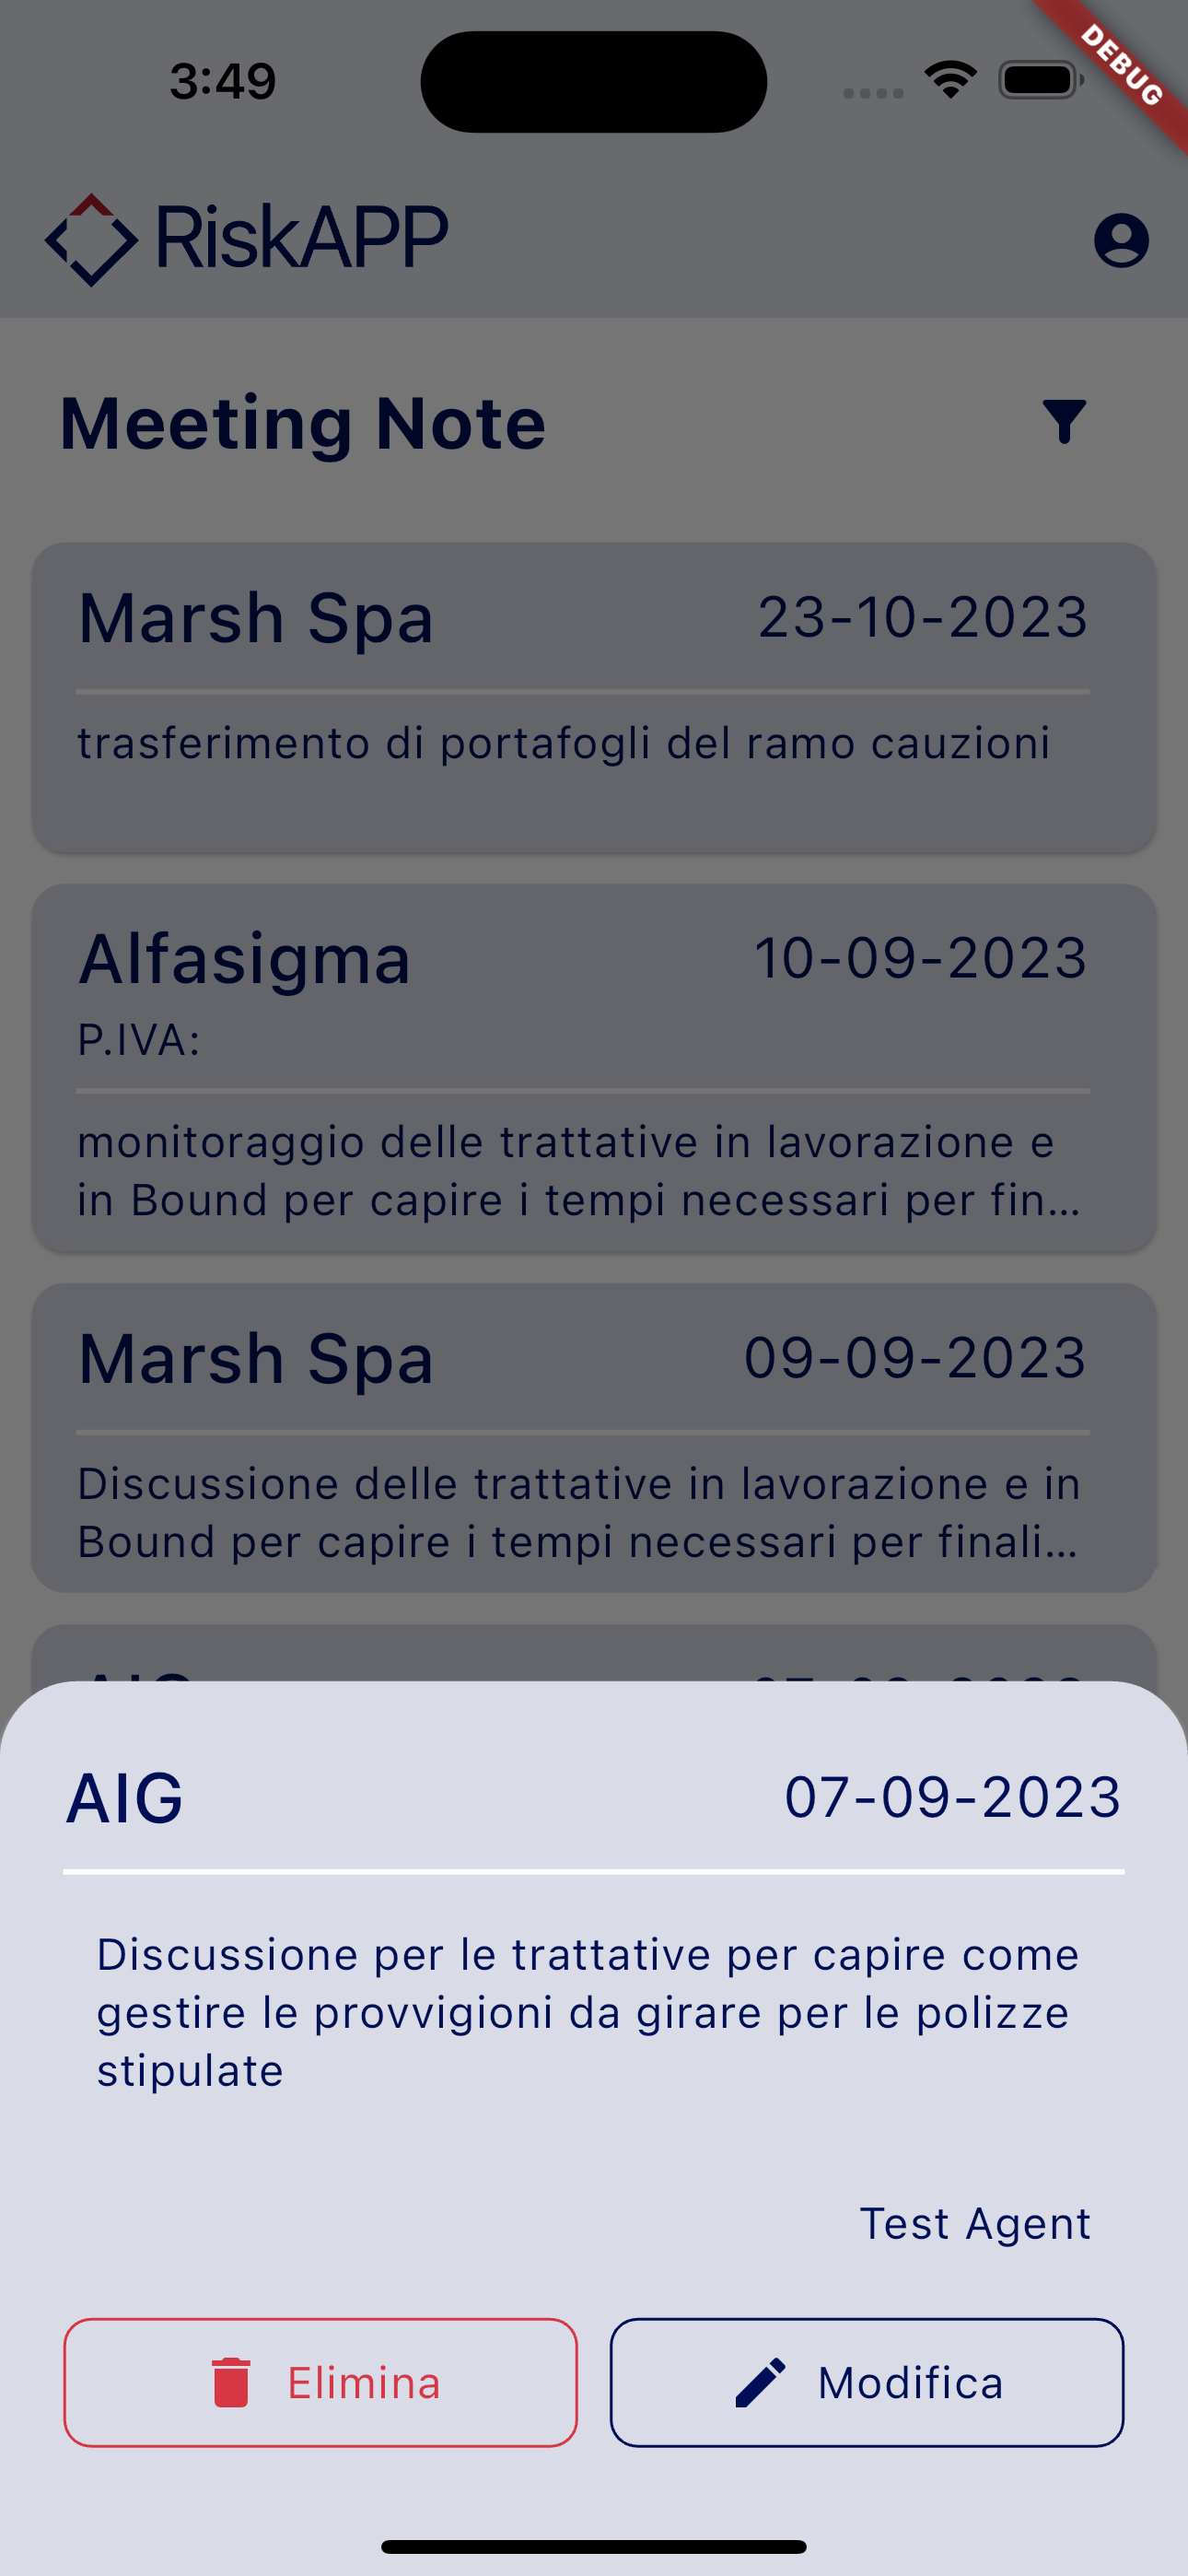
\includegraphics[width=0.3\columnwidth]{screenshot/13-meeting_note} 
    \caption{\emph{Meeting Note Card}}
    \label{fig:meeting-note-card}
\end{figure}

\subsection{Object Picker}
\label{subsec:object-picker}

Nel file denominato \lstinline{object_picker.dart} è stato implementato \lstinline{CustomObjectPicker}, classe che estende un \lstinline{StatefulWidget} per costruire un componente in grado di permettere all'utente di selezionare la categoria dei clienti. \\
Viene utilizzato all'interno del \emph{Filter Panel} (sezione \ref{subsec:filter-panel}), dal \emph{wizard} di creazione/modifica di una \emph{Meeting Note} (sezione \ref{subsec:wizard-screen-1}) e nella schermata di revisione per la creazione automatica di una \emph{Meeting Note} (sezione \ref{subsec:smart-creation-screen}).\\
Anche per questo componente si è pensato di rivisitarlo rispetto al \gls{mockup}\glsoccur, in quanto si è deciso di utilizzare un \lstinline{CupertinoPicker}\cite{site:cupertino-picker}, che visualizza le categorie dei clienti selezionabili, passate in input attraverso il costruttore, al posto di un \lstinline{DropdownMenu}\cite{site:dropdown-menu}, questo per favorire l'utilizzo dell'applicazione da parte di utenti in mobilità, poichè il primo appare dal basso e dunque diventa più facilmente raggiungibile (figura \ref{fig:object-picker}). \\
Inoltre sono stati definiti dei metodi che permettono di ottenere la categoria selezionata attraverso l'indice e di aggiornare lo stato del \emph{widget} al cambiamento di quest'ultima.

\begin{figure}[!h] 
    \centering 
    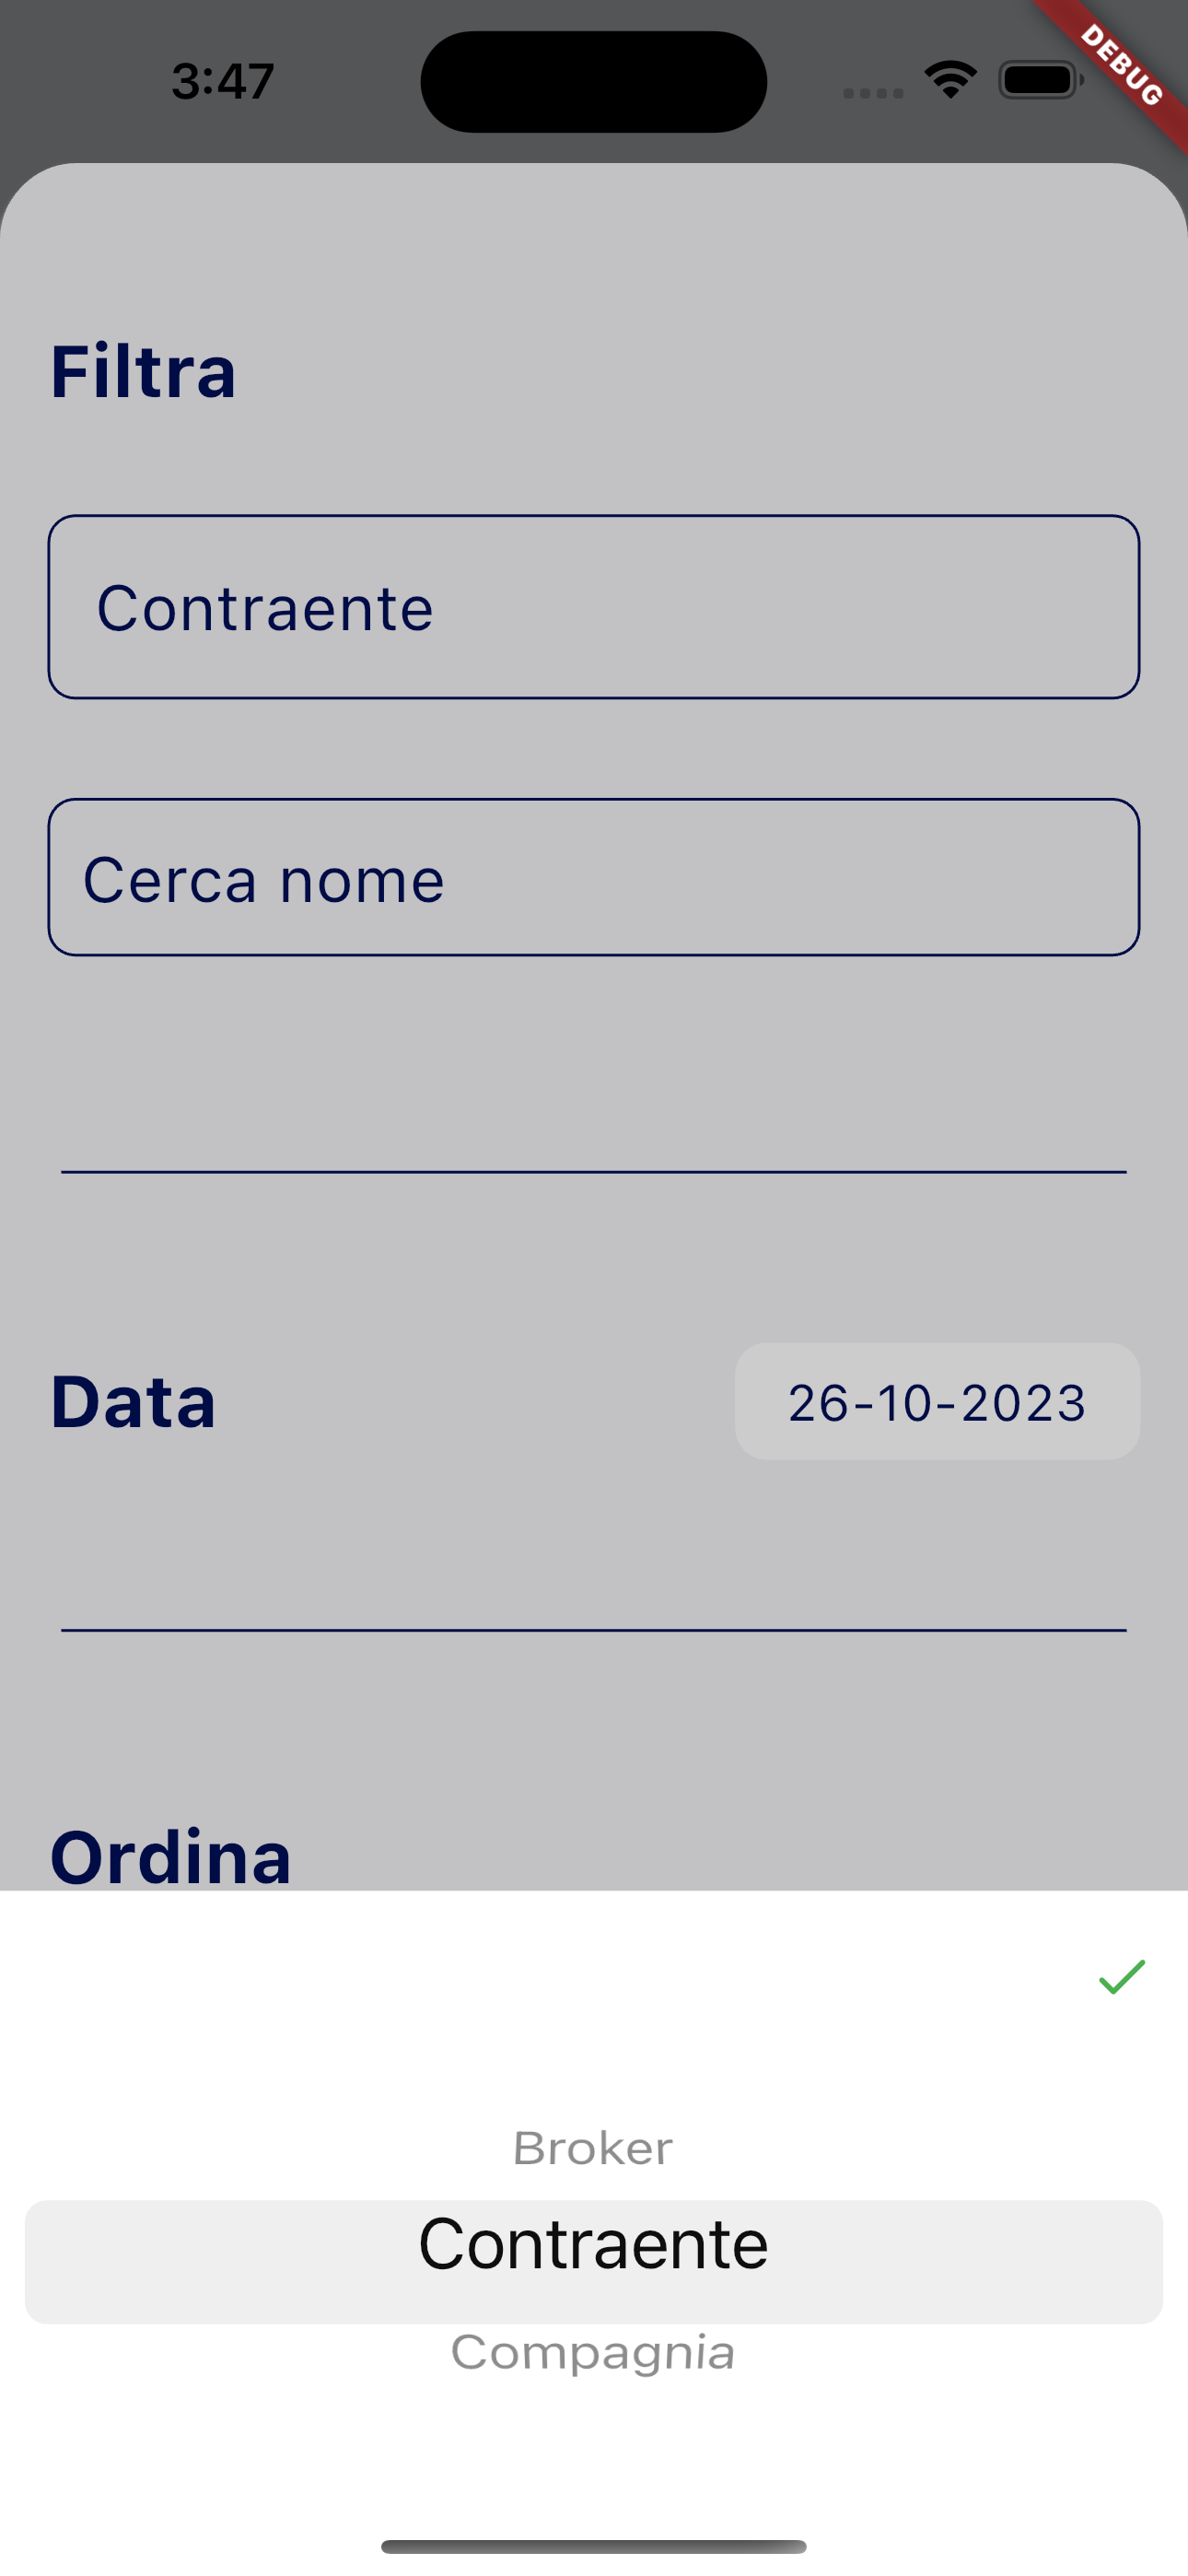
\includegraphics[width=0.3\columnwidth]{screenshot/9-object_picker}
    \caption{Selettore di categoria dei clienti}
    \label{fig:object-picker}
\end{figure}

\subsection{Recording Button}
\label{subsec:recording-button}

Nel file denominato \lstinline{recording_button.dart} è stato implementato un \lstinline{StatelessWidget} per costruire un componente in grado di permettere all'utente di attivare la dettatura vocale ( requisito \hyperref[RFN-73]{RFN-73}).\\
È composto da un \lstinline{Text}\cite{site:text} che esplicita all'utente lo scopo del pulsante, da un \lstinline{IconButton}\cite{site:icon-button} e da un \lstinline{AvatarGlow}\cite{site:avatar-glow} per rappresentare l'animazione che viene visualizzata quando la dettatura vocale è attiva.\\
L'attivazione avviene in base al valore della variabile \lstinline{bool} \lstinline{isRecording} che viene passata attraverso il costruttore, come anche il comportamento del pulsante, definito attraverso il metodo \lstinline{onPressed}\cite{site:on-pressed}.

\begin{figure}[!h] 
    \centering 
    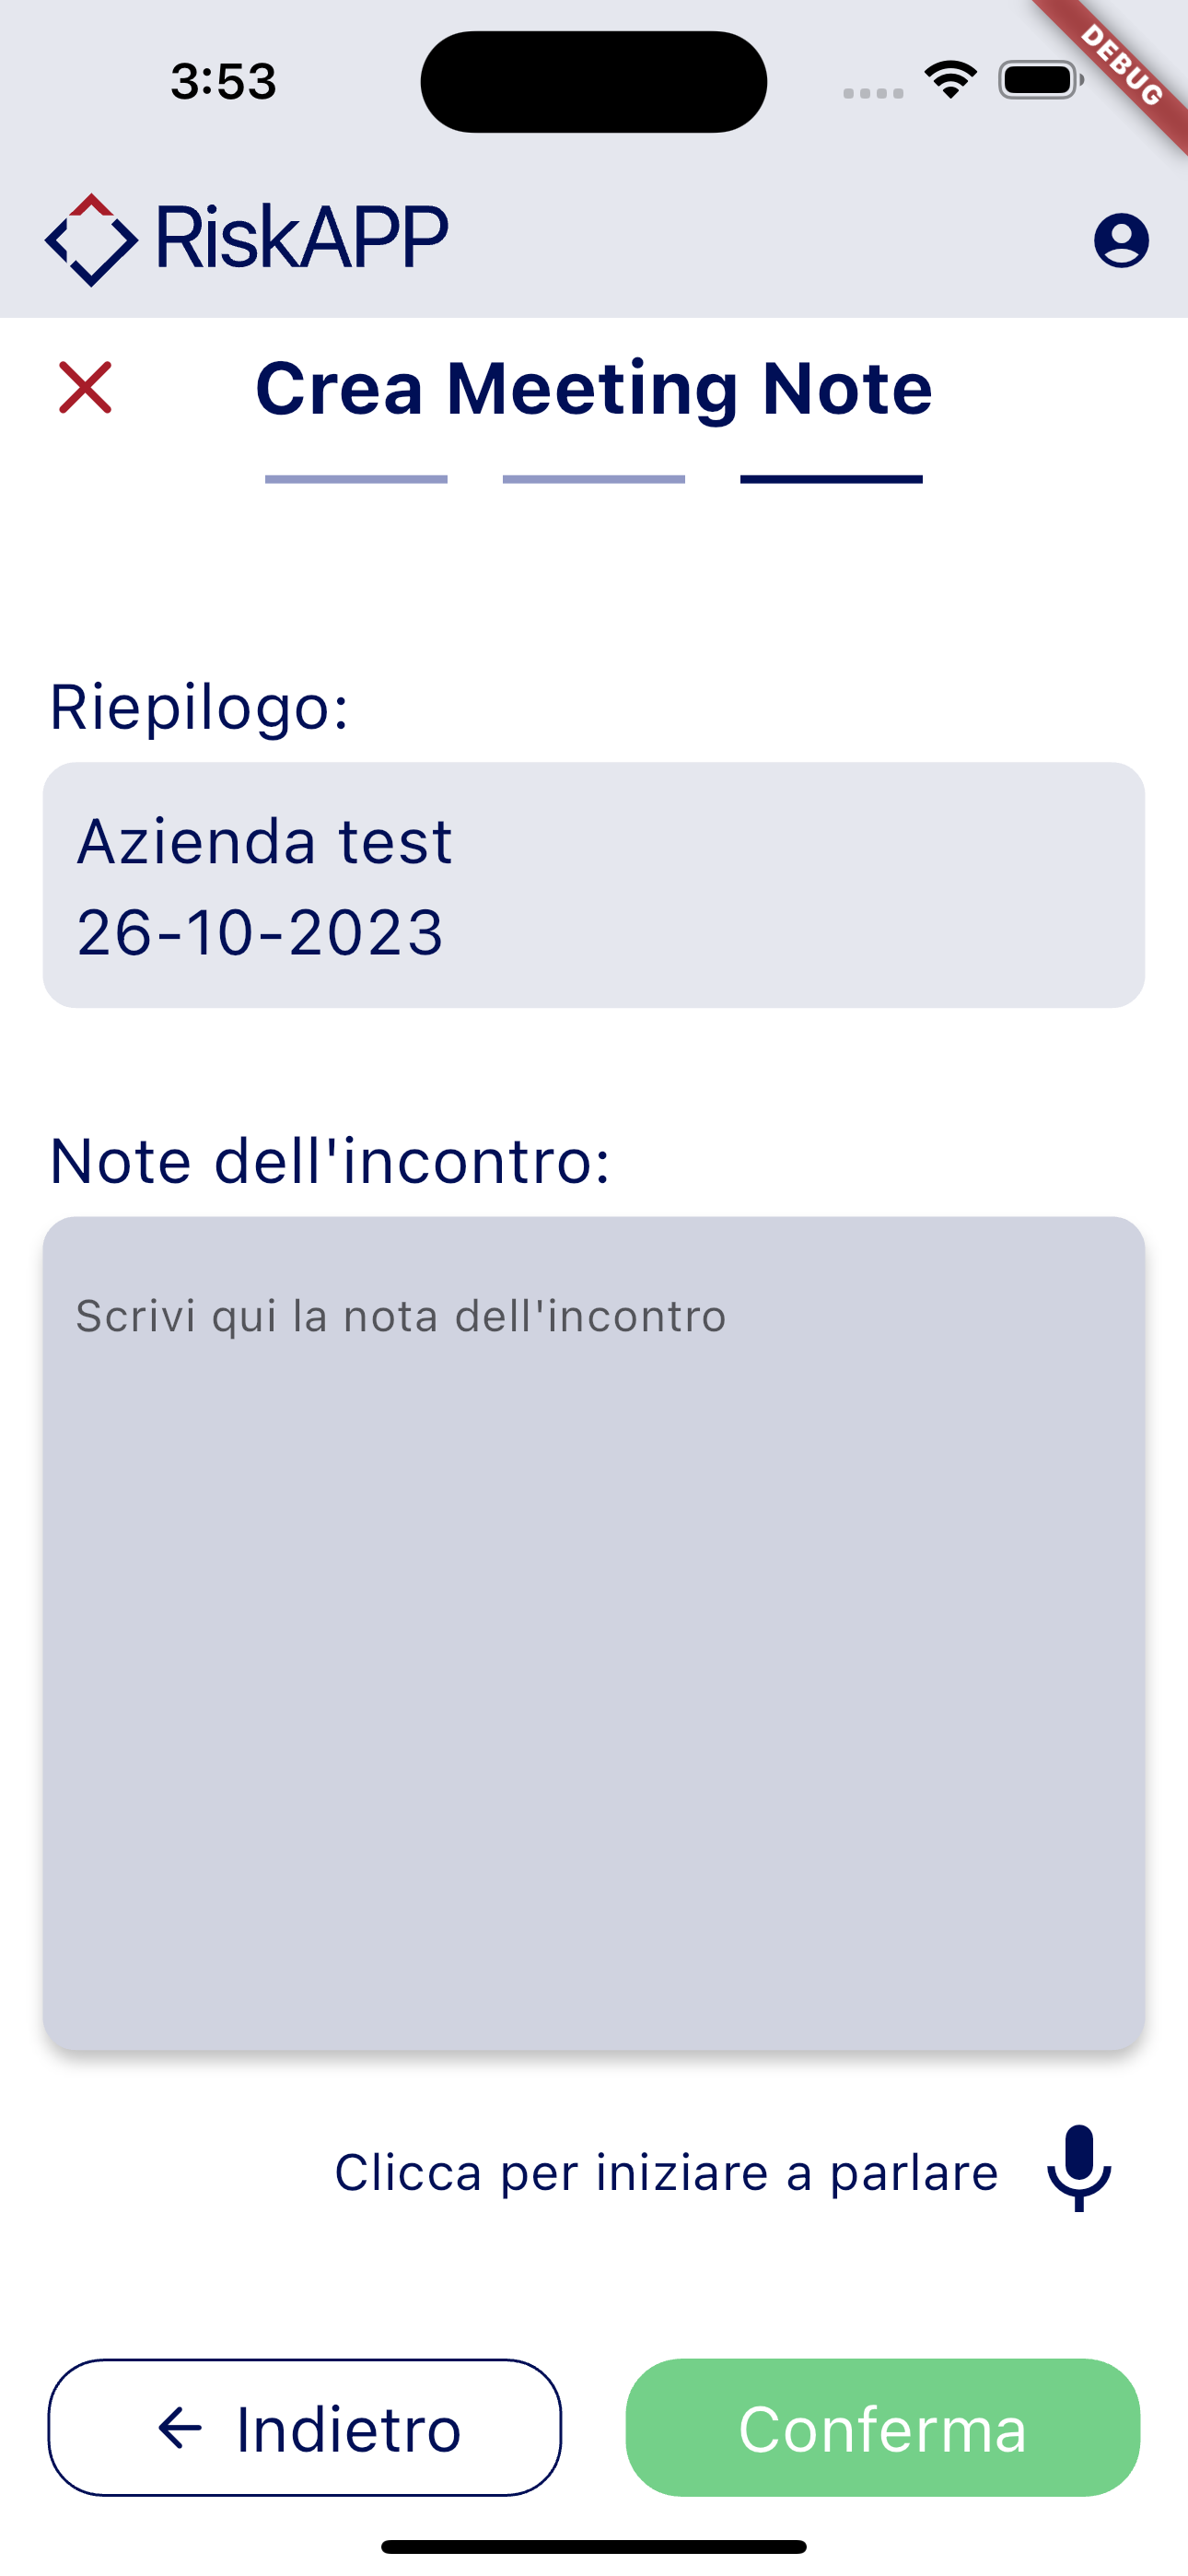
\includegraphics[width=0.3\columnwidth]{screenshot/20-wc3}
    \hfill
    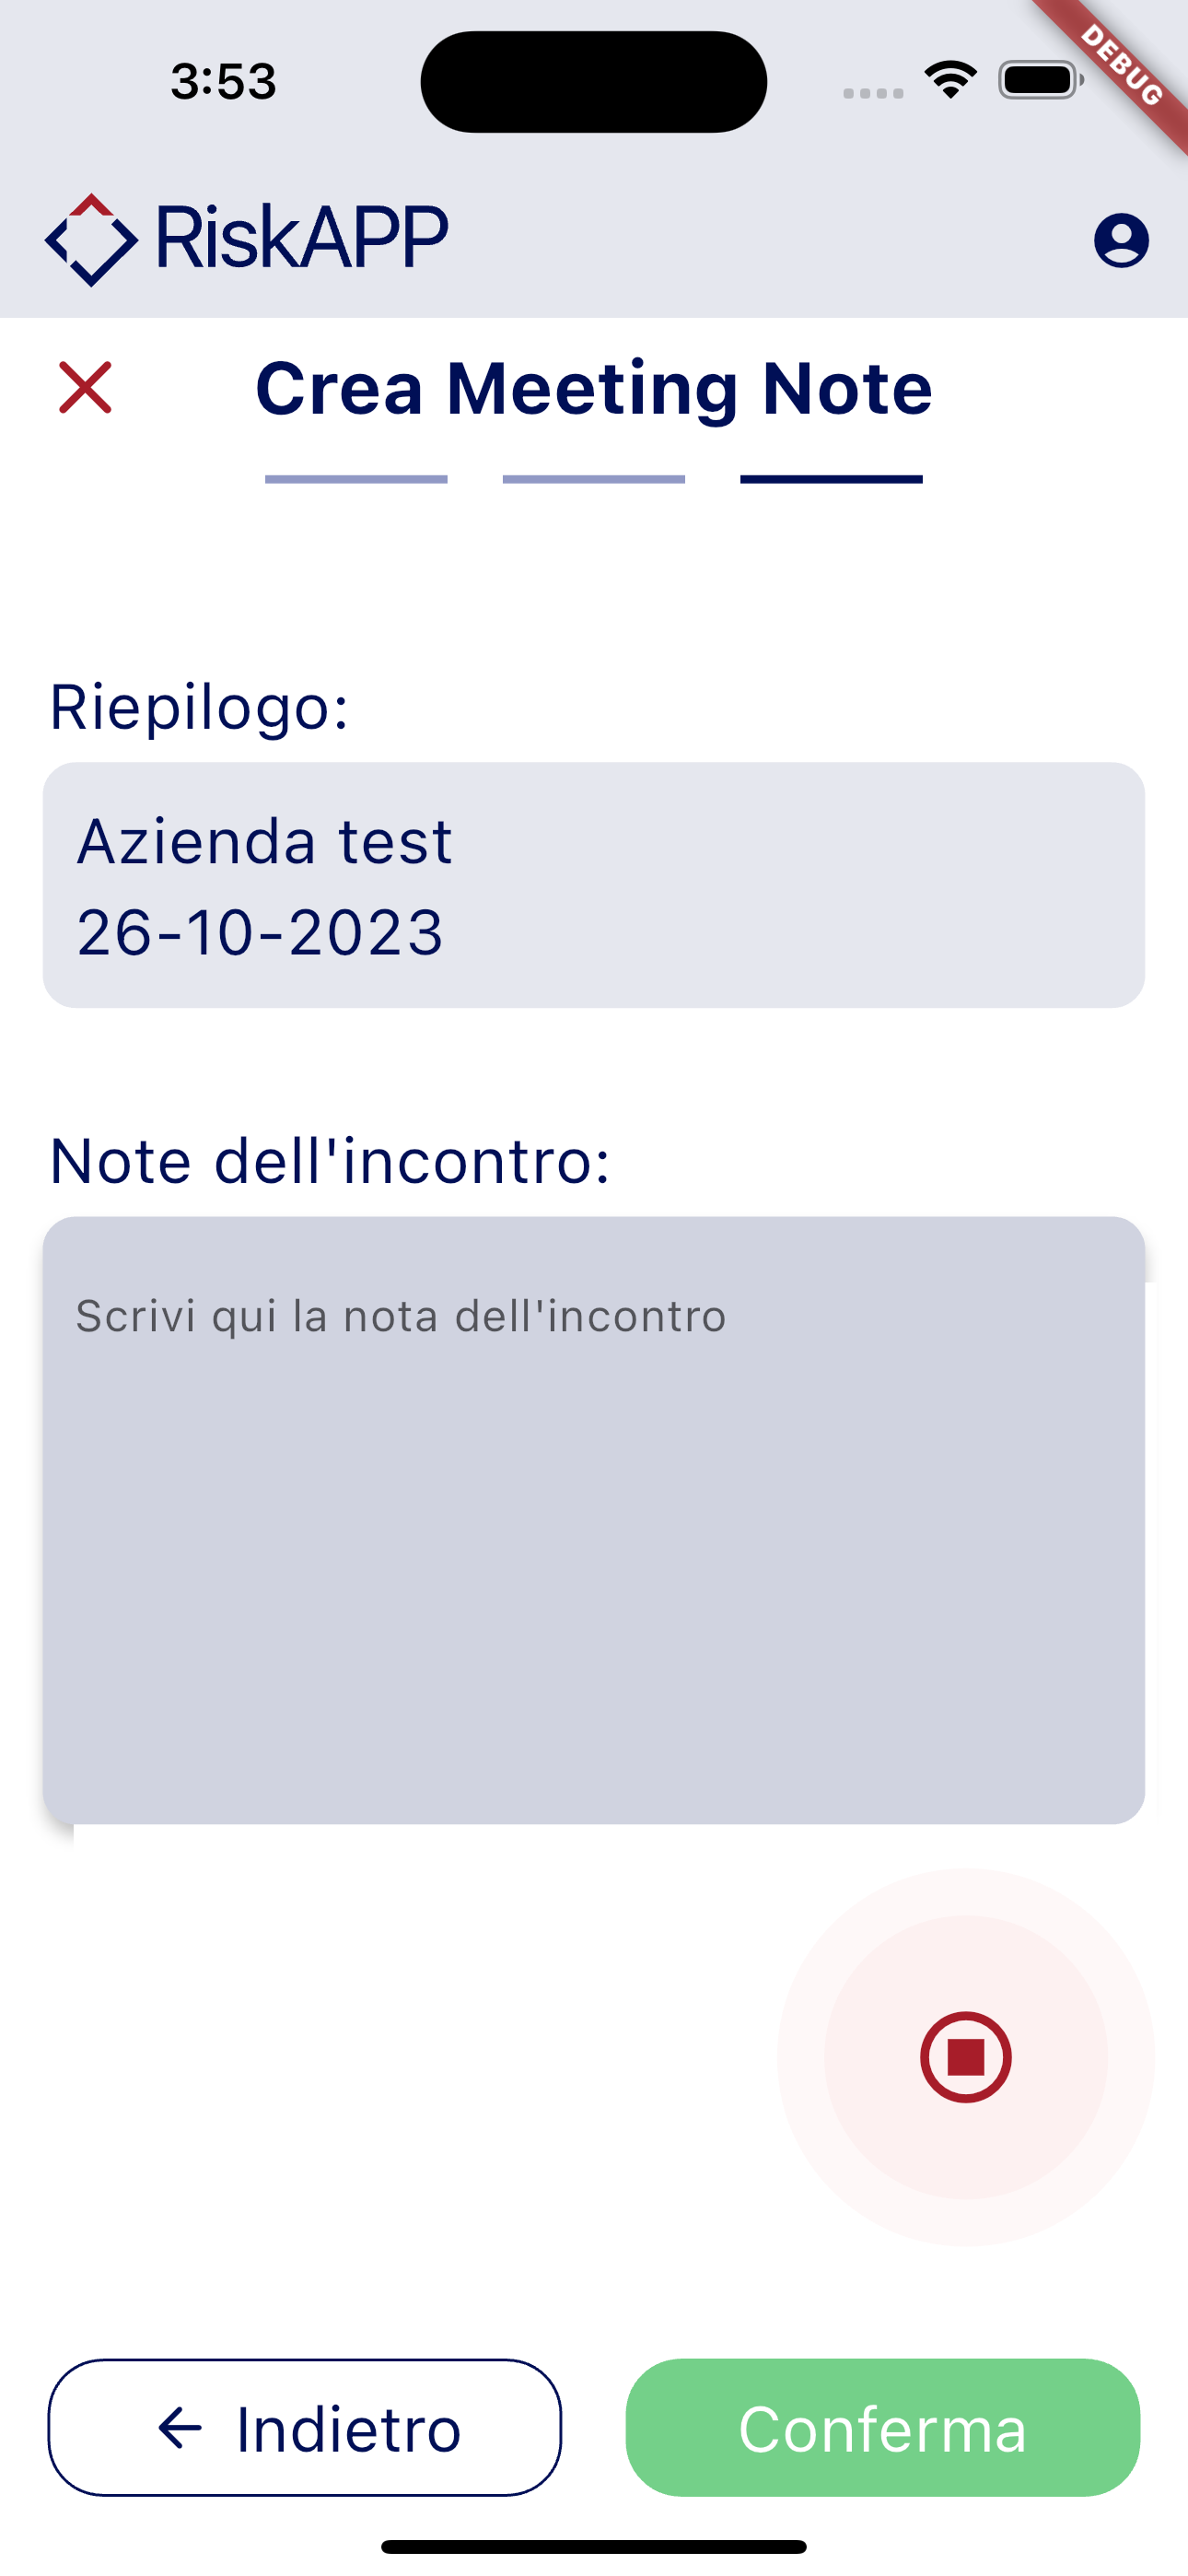
\includegraphics[width=0.3\columnwidth]{screenshot/21-wc3_record} 
    \caption{Pulsante rispettivamente nello stato di non attivazione e attivazione della dettatura vocale}
    \label{fig:record-button}
\end{figure}

\newpage

\subsection{Screens Template}
\label{subsec:screens-template}

Nel file denominato \lstinline{screens_template.dart} sono stati implementati dei \lstinline{StatelessWidget} per costruire diversi componenti che rappresentano gli elementi comuni per la struttura delle schermate dell'applicazione.

\subsubsection*{BaseScreen}
\label{subsubsec:base-screen}

Classe in cui viene definito la struttura e l'aspetto base che dovranno avere tutte le schermate dell'applicazione.\\
È composto da un \lstinline{Scaffold}\cite{site:scaffold}, contenitore principale di tutti gli elementi grafici, in cui viene applicato il tema dell'applicazione (sezione \ref{subsec:app-theme}). \\
Sono state definite poi varie proprietà di base dello \lstinline{Scaffold}, tra cui \lstinline{appBar} con \lstinline{CustomAppBar} (sezione \ref{subsubsec:custom-app-bar}) e un \lstinline{body}, passato per parametro del costruttore, in quanto ogni schermata ha il suo contenuto.\\
È stata inoltre definita la proprietà \lstinline{bottomNavigationBar} che non viene utilizzata da tutte le schermate, ma vi è comunque la possibilità di implementarla nel caso cui si vogliano aggiungere dei pulsanti di navigazione nella parte inferiore della vista per avanzare o retrocedere tra le varie schermate dell'applicazione.\\
Per abilitare tali pulsanti è sufficiente passare, a seconda delle necessità, un \emph{widget} \lstinline{forwardButton} per la progressione e/o \lstinline{backButton} per la retrocessione.

\subsubsection*{WizardScreen}
\label{subsubsec:wizard-screen}

Classe che implementa \lstinline{BaseScreen} e che si occupa di fornire un \emph{template} per le schermate che compongono il \gls{wizard}\glsoccur di creazione/modifica di una \emph{Meeting Note} (figure \ref{fig:w1}, \ref{fig:w2} e \ref{fig:w3}).\\
Imposta a \lstinline{true} la proprietà \lstinline{enableIcon} per mantenere il pulsante di accesso alla schermata dell'account utente.\\
Attraverso i parametri del costruttore è obbligatorio passare il \lstinline{body}, mentre sono opzionali \lstinline{forwardButton} e \lstinline{backButton}.

\subsubsection*{WizardHeader}
\label{subsubsec:wizard-header}

Classe che definisce l'aspetto grafico dell'\emph{header} del \gls{wizard}\glsoccur di creazione/modifica di una \emph{Meeting Note}.\\
É composto da un \lstinline{Text}\cite{site:text} che rappresenta il titolo della schermata e da un \lstinline{IconButton}\cite{site:icon-button}, ha lo scopo di mostrare un \lstinline{WarningAlertDialog} (sezione \ref{subsubsec:warning-alert-dialog}) chiedendo all'utente se vuole abbandonare il \gls{wizard}\glsoccur, in caso affermativo viene mostrata la schermata principale dell'applicazione, altrimenti viene chiusa la modale (figura \ref{fig:wizard-header}). 

\begin{figure}[!h] 
    \centering 
    
\includegraphics[width=0.3\columnwidth]{screenshot/42-wizard_header} 
    \caption{Applicazione di \emph{WizardHeader}}
    \label{fig:wizard-header}
\end{figure}

\subsubsection*{WizardStepper}
\label{subsubsec:wizard-stepper}

Classe che è composta da tre \lstinline{Step} (sezione \ref{subsubsec:step}), il numero massimo di passi pensato per il \gls{wizard}\glsoccur, inoltre riceve in input il numero di passo corrente in modo da evidenziare a che punto l'utente si trova nella progressione.
Si specifica che \lstinline{WizardStepper} è privato, è stato infatti creato con lo scopo di essere utilizzato esclusivamente all'interno di questo \emph{widget} (figura \ref{fig:wizard-stepper}).\\

\begin{figure}[!h] 
    \centering 
    
\includegraphics[width=0.3\columnwidth]{screenshot/41-wizard_stepper} 
    \caption{Applicazione di \emph{WizardStepper}}
    \label{fig:wizard-stepper}
\end{figure}

\subsubsection*{Step}
\label{subsubsec:step}

Classe che definisce l'aspetto grafico di un passo del \gls{wizard}\glsoccur di creazione/modifica di una \emph{Meeting Note}.\\
Sostanzialmente consiste in un \lstinline{Divider}\cite{site:divider} che rappresenta un passo, definendo due colori diversi per evidenziare quello in cui l'utente si trova da quelli precedenti e/o successivi.

\subsection{Scroll Date Picker}
\label{subsec:scroll-date-picker}

Nel file denominato \lstinline{scroll_date_picker.dart} è stata definita la classe \lstinline{CustomScrollDatePicker} che estende \lstinline{StatefulWidget} per costruire un componente in grado di permettere all'utente di selezionare una data, nel momento di creazione/modifica di una \emph{Meeting Note} (figura \ref{fig:w2}).\\
È composto da un \lstinline{Text}\cite{site:text} che visualizza la data selezionata, un \lstinline{ScrollDatePicker}\cite{site:scroll-date-picker} e un pulsante che reimposta la data selezionata a quella corrente (figura \ref{fig:w2}).\\
Espone dei metodi che permettono di ottenere la data selezionata con \lstinline{selectedDate}, e di aggiornare lo stato del \emph{widget} al cambiamento di quest'ultima con \lstinline{onDateChanged}.

\subsection{Search Bar}
\label{subsec:search-bar}

Nel file denominato \lstinline{search_bar.dart} sono stati implementati dei \emph{widget} che estendono \lstinline{StatelessWidget} per costruire dei componenti in grado di permettere all'utente di effettuare una ricerca.

\subsubsection*{CustomSearchBar}
\label{subsubsec:custom-search-bar}

Classe che implementa una \lstinline{SearchBar}\cite{site:search-bar} in cui viene definito pressochè solo l'aspetto grafico in quanto attraverso il costruttore è obbligatorio passare un \lstinline{TextEditingController}\cite{site:text-editing-controller}, che si occupa di gestire il testo inserito dall'utente, e un metodo \lstinline{onChanged} che gestisce l'evento di cambiamento del testo inserito dall'utente, mentre è opzionale passare il colore del \emph{background} del componente. \\
Lo scopo è quello di fornire all'utente la possibilità di effettuare una ricerca all'interno della lista dei clienti (figura \ref{fig:w1}).

\subsubsection*{CustomAutocomplete}
\label{subsubsec:custom-autocomplete}

Classe che implementa \lstinline{Autocomplete}\cite{site:autocomplete}, consente di fornire dei suggerimenti per l'autocompletamento nella ricerca, in cui viene anche qui definito solo l'aspetto grafico. \\
Attraverso il costruttore si rende necessario passare dei metodi fondamentali: \lstinline{optionsBuilder} che fornisce i suggerimenti per l'autocompletamento, \lstinline{displayStringForOption} che definisce quale attributo dell'oggetto suggerito visualizzare e \lstinline{onSelected} che si occupa di gestire l'evento di selezione di un suggerimento.\\
Viene impiegato nel \emph{widget} \lstinline{FilterPanel} (sezione \ref{subsec:filter-panel}) per fornire all'utente la possibilità di ricercare un cliente e nella scherma di conferma per la creazione automatica di una \emph{Meeting Note} (sezione \ref{subsec:smart-creation-screen})

\begin{figure}[!h] 
    \centering 
    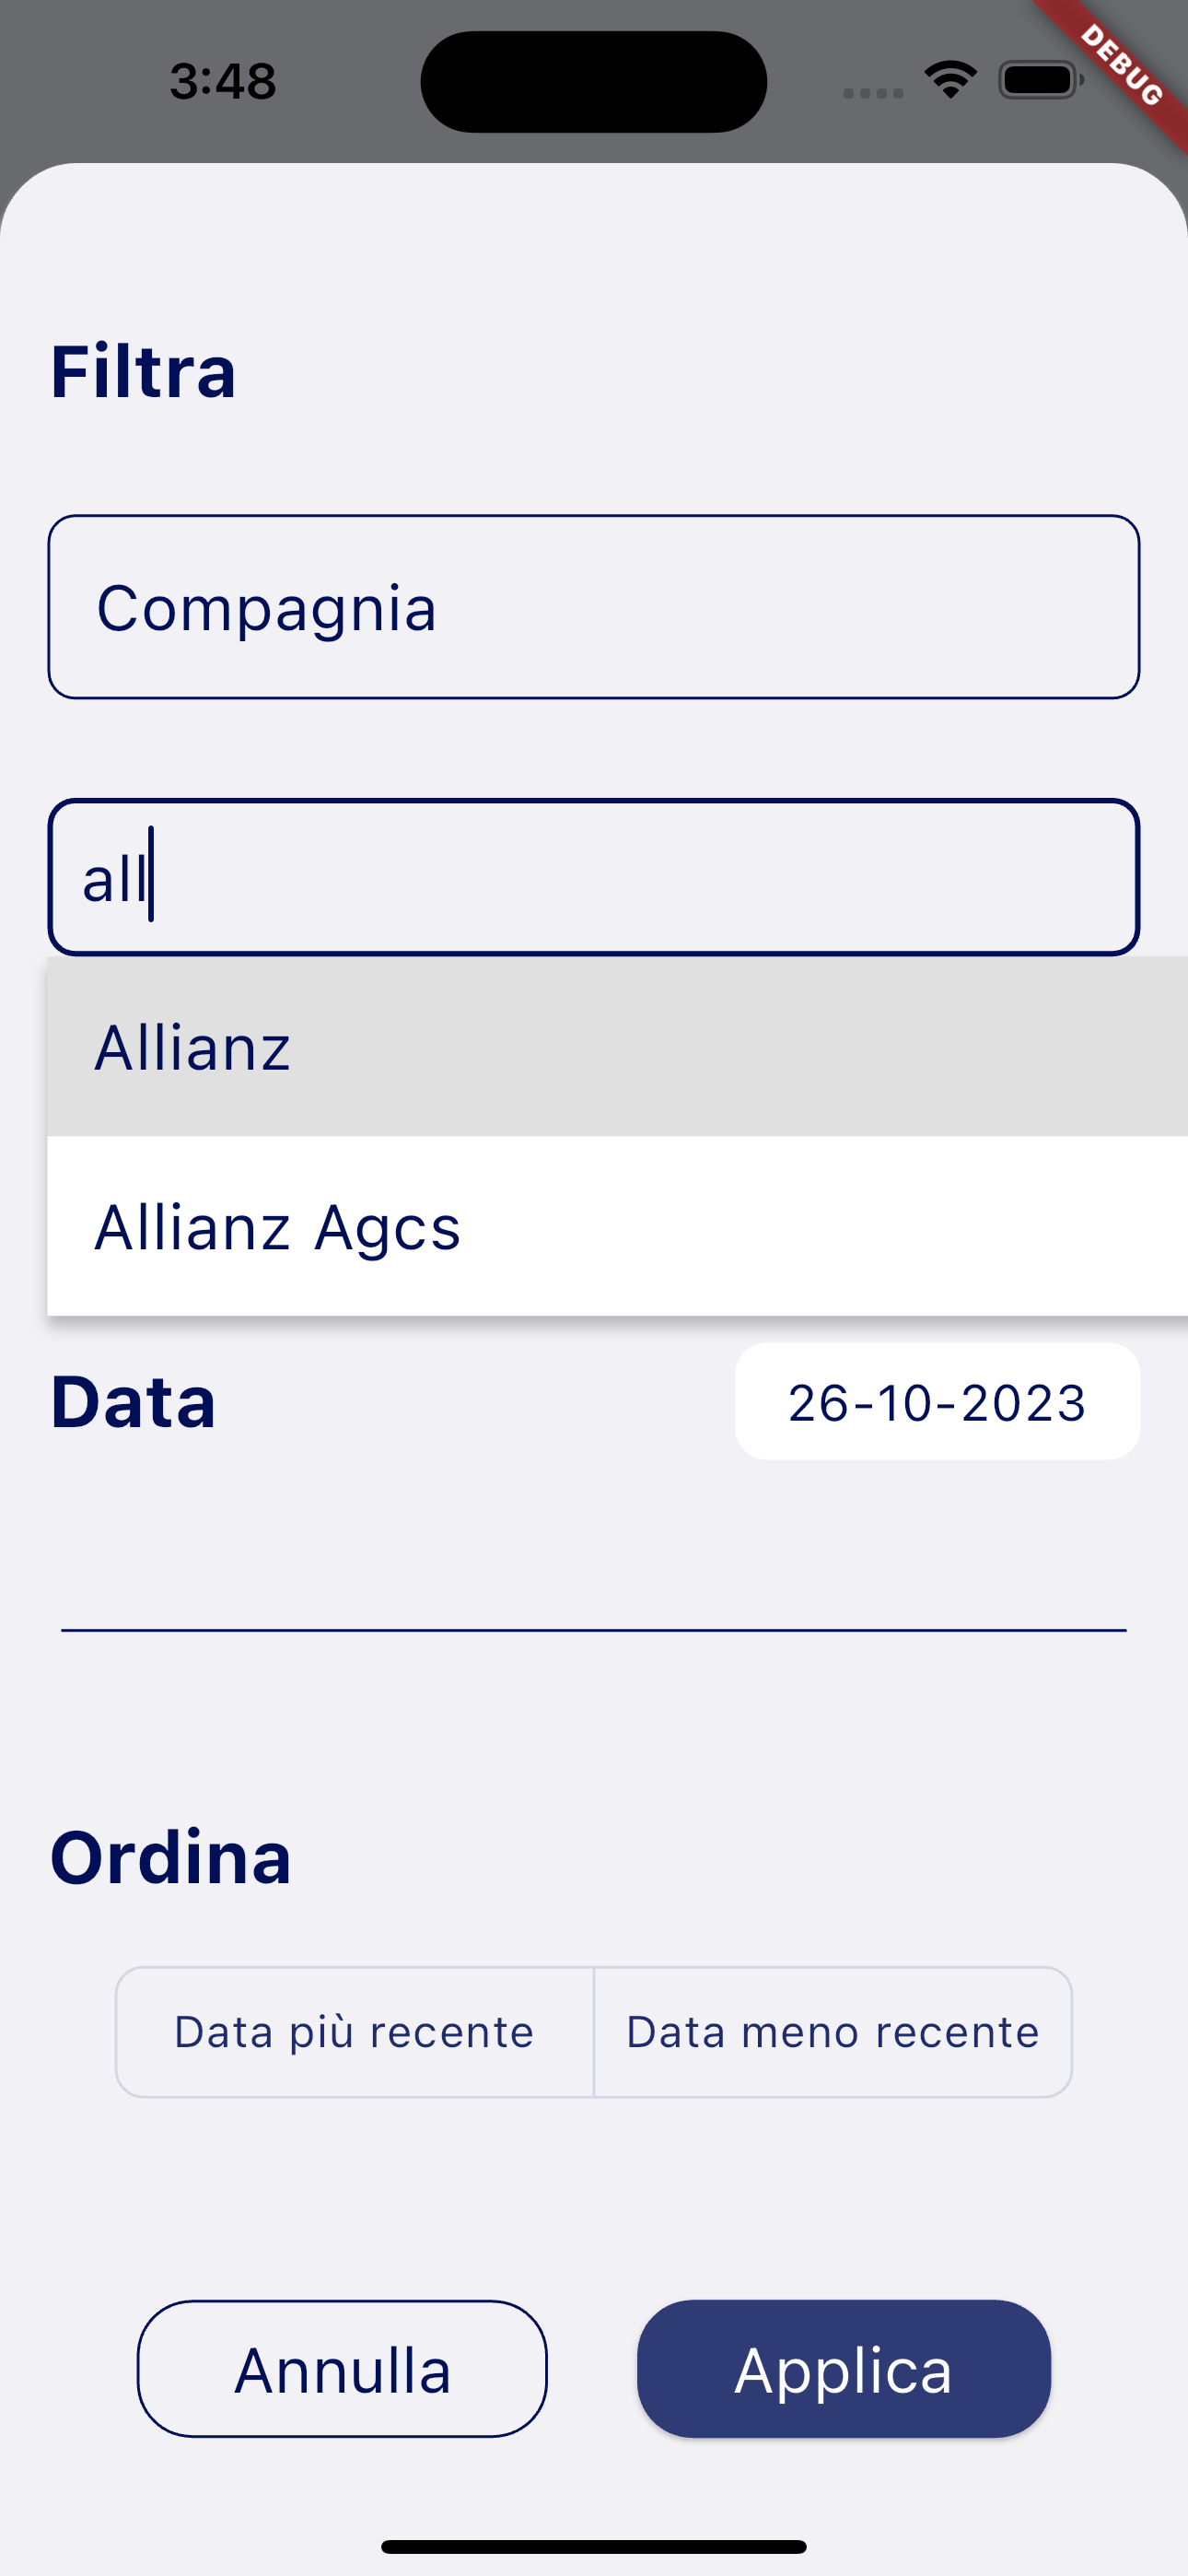
\includegraphics[width=0.3\columnwidth]{screenshot/10-autcomplete} 
    \caption{Applicazione di \emph{Autocomplete}}
    \label{fig:autocomplete}
\end{figure}

\subsection{Text Box}
\label{subsec:text-box}

Nel file denominato \lstinline{text_box.dart} è stato implementato un \lstinline{StatefulWidget} per costruire un componente in grado di permettere all'utente di inserire del testo.\\
È composto da semplicemente un \lstinline{TextField}\cite{site:text-field} in cui viene personalizzato nell'aspetto grafico, è richiesto dal costruttore il passagio dell'altezza di questo componente, in modo da poterlo utilizzare in diverse situazioni, poi è necessatio passare un \lstinline{TextEditingController}\cite{site:text-editing-controller} e un metodo \lstinline{onChanged} che si occupa di gestire l'evento di cambiamento del testo inserito dall'utente.\\
Viene utilizzato per la creazione/modifica di una \emph{Meeting Note} e per la creazione automatica.

\begin{figure}[!h] 
    \centering 
    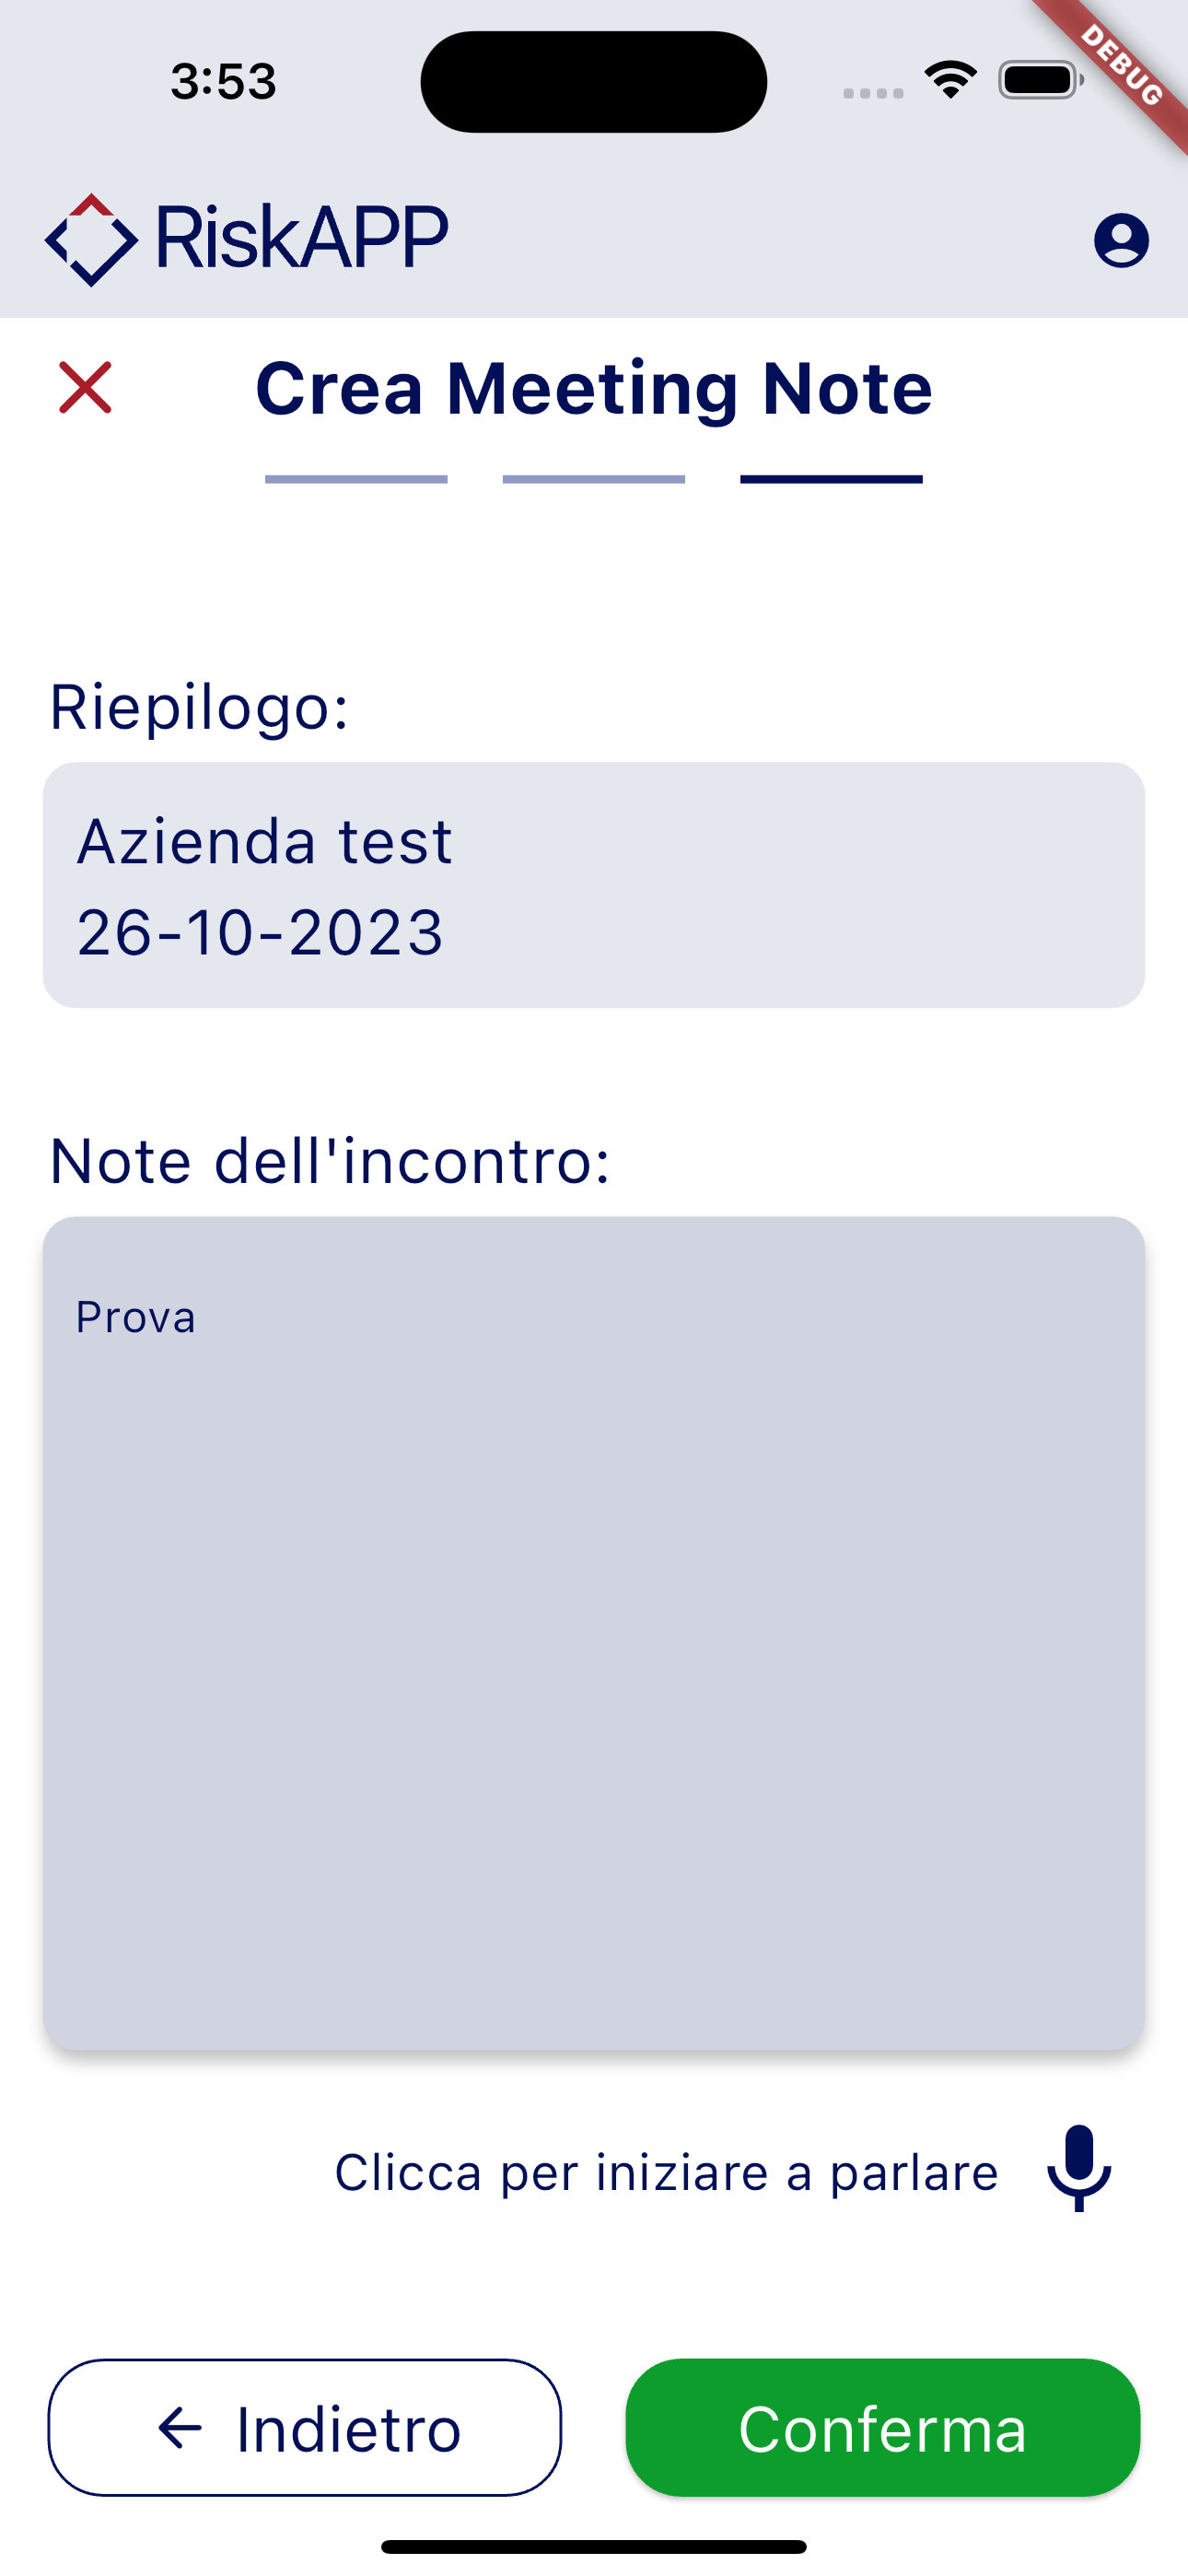
\includegraphics[width=0.3\columnwidth]{screenshot/22-wc3_textbox} 
    \caption{Applicazione di \emph{TextBox}}
    \label{fig:text-box}
\end{figure}

\subsection{Toogle Buttons}
\label{subsec:toogle-buttons}

Nel file denominato \lstinline{toogle_buttons.dart} è stato implementato un \lstinline{StatefulWidget} per costruire un componente in grado di permettere all'utente di selezionare una delle due opzioni disponibili.\\
È composto da un \lstinline{ToggleButtons}\cite{site:toggle-buttons} di cui viene definito l'aspetto grafico e il comportamento.\\
Attraverso il costruttore è necessario passare un \lstinline{List<Widget>} contenente le due opzioni disponibili, un \lstinline{List<bool>} che indica quale opzione è stata selezionata e un metodo \lstinline{onChoiceSelected} che si occupa di gestire l'evento di selezione di un'opzione.\\
Viene impiegato nel \lstinline{FilterPanel} (sezione \ref{subsec:filter-panel}) per fornire all'utente la possibilità di selezionare una delle due opzioni disponibili per filtrare la lista di \emph{Meeting Note}.

\begin{figure}[!h] 
    \centering 
    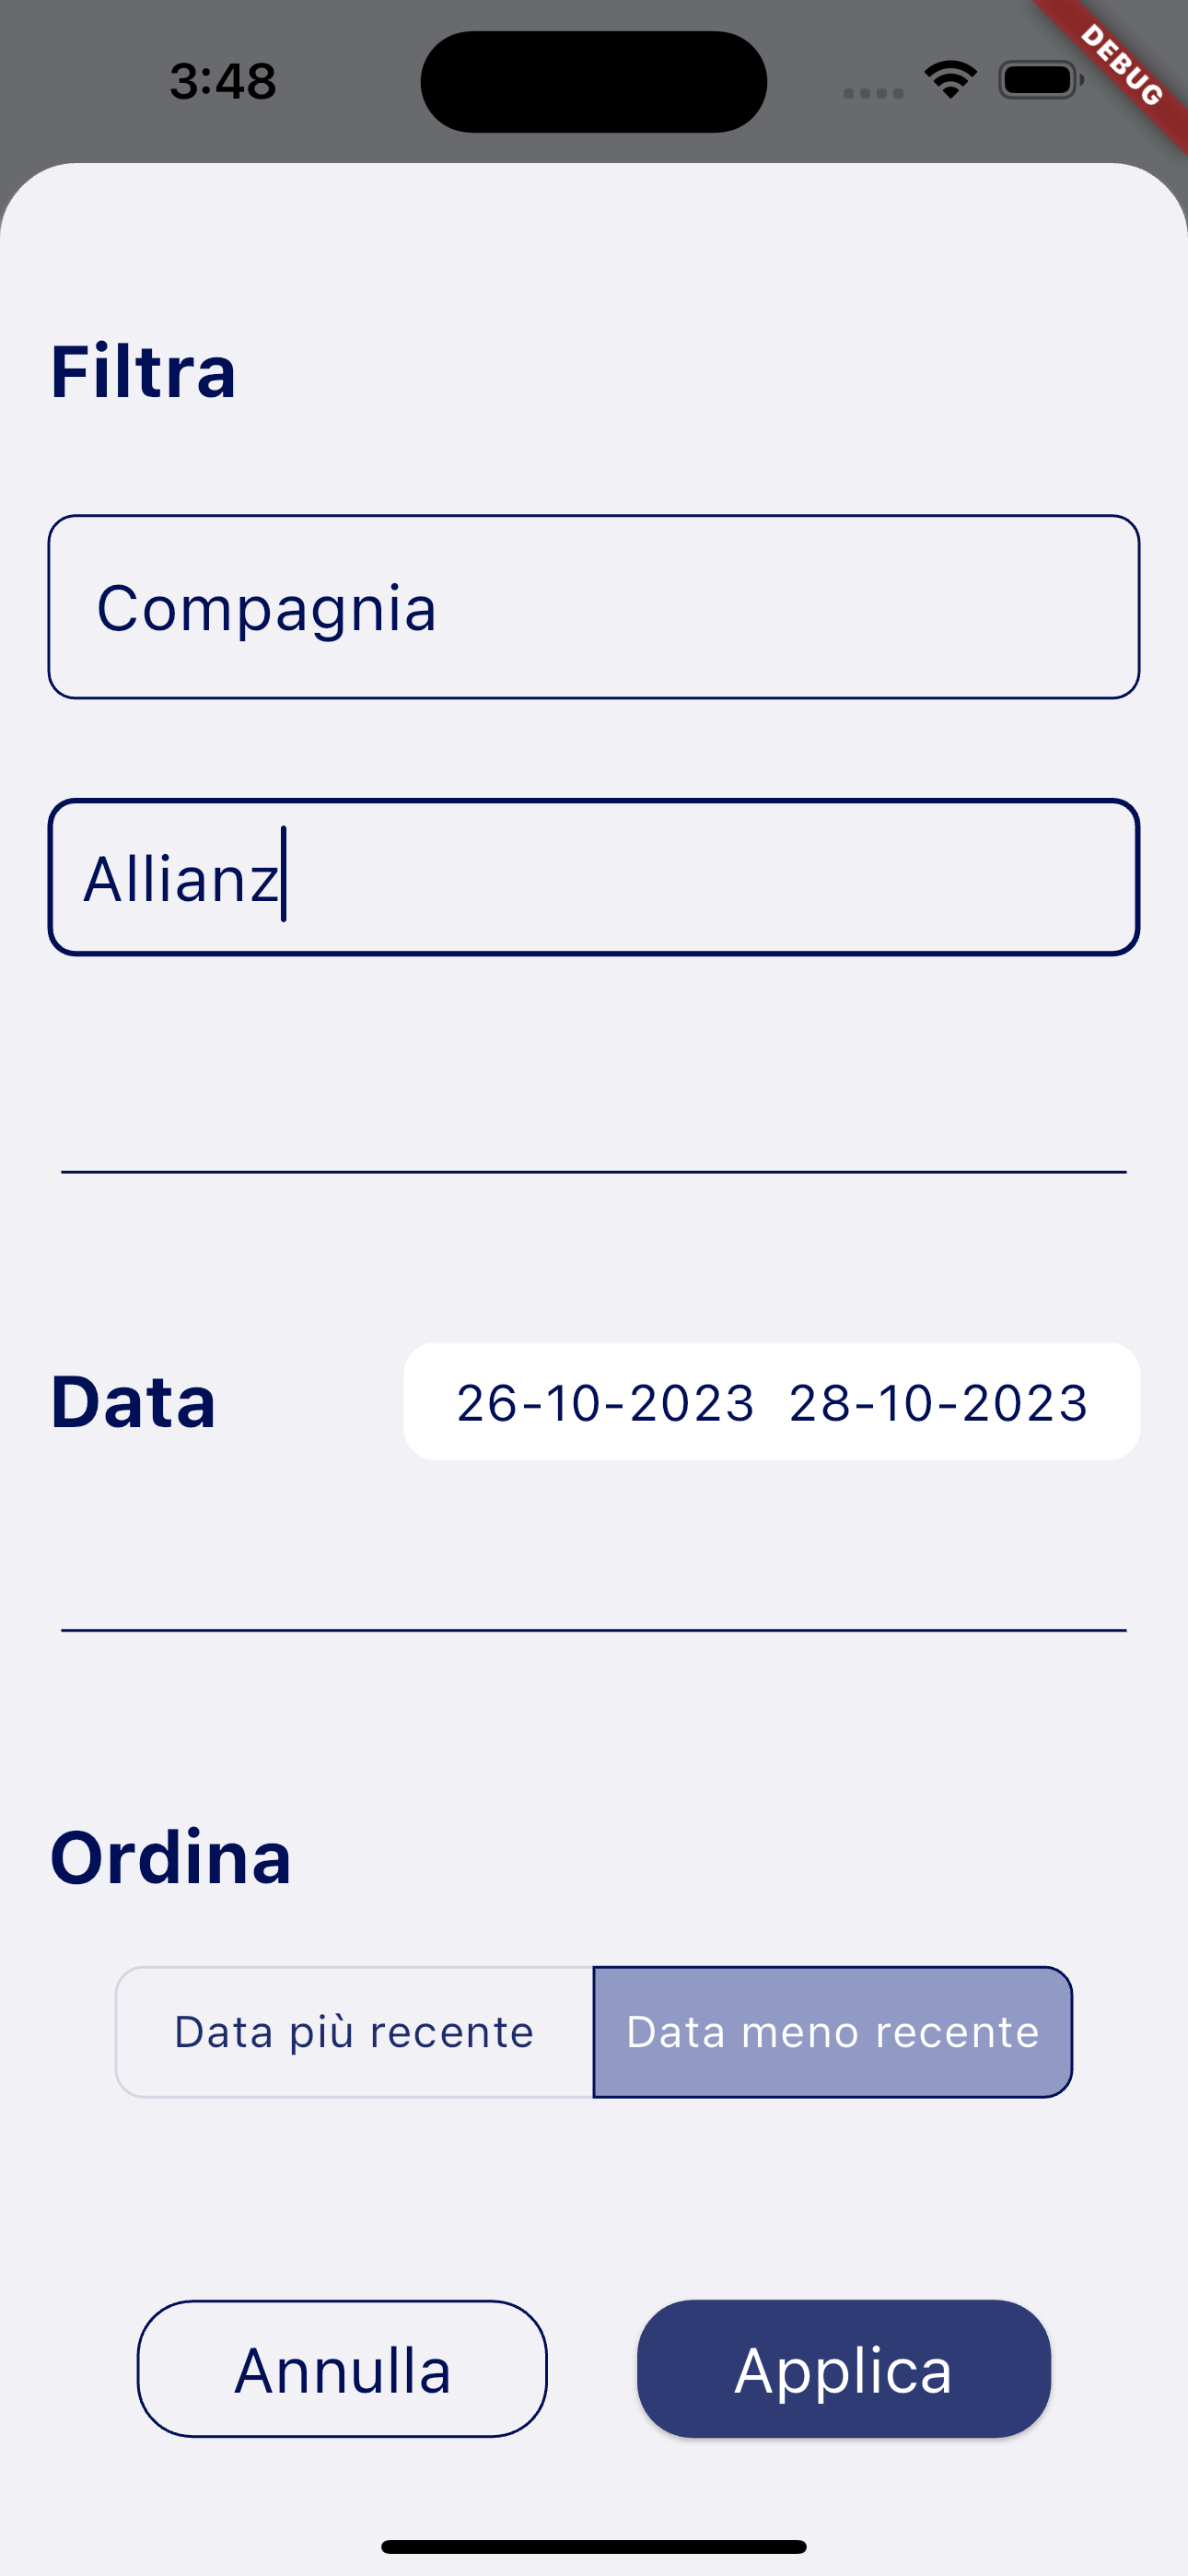
\includegraphics[width=0.3\columnwidth]{screenshot/12-toggle_buttons} 
    \caption{Applicazione di \emph{ToggleButtons}}
    \label{fig:toggle-button}
\end{figure}

\clearpage

\subsection{Warning Alert}
\label{subsec:warning-alert}

Nel file denominato \lstinline{warning_alert.dart} è stato implementato un \lstinline{StatelessWidget} per costruire un componente composto da un \lstinline{Text}\cite{site:text} e un \lstinline{Icon}\cite{site:icon}, il loro scopo è quello di visualizzare il messaggio di avvertimento, attraverso i parametri del costruttore viene passato il messaggio e il colore che devono avere il testo e l'icona.\\
I casi in cui viene richiesto si faccia riferimento ai seguenti requisiti: \hyperref[RFN-12]{RFN-12}, \hyperref[RFN-13]{RFN-13}, \hyperref[RFN-20]{RFN-20}, \hyperref[RFN-30]{RFN-30}, \hyperref[RFN-34]{RFN-34}, \hyperref[RFN-64]{RFN-64}.

\begin{figure}[!h] 
    \centering 
    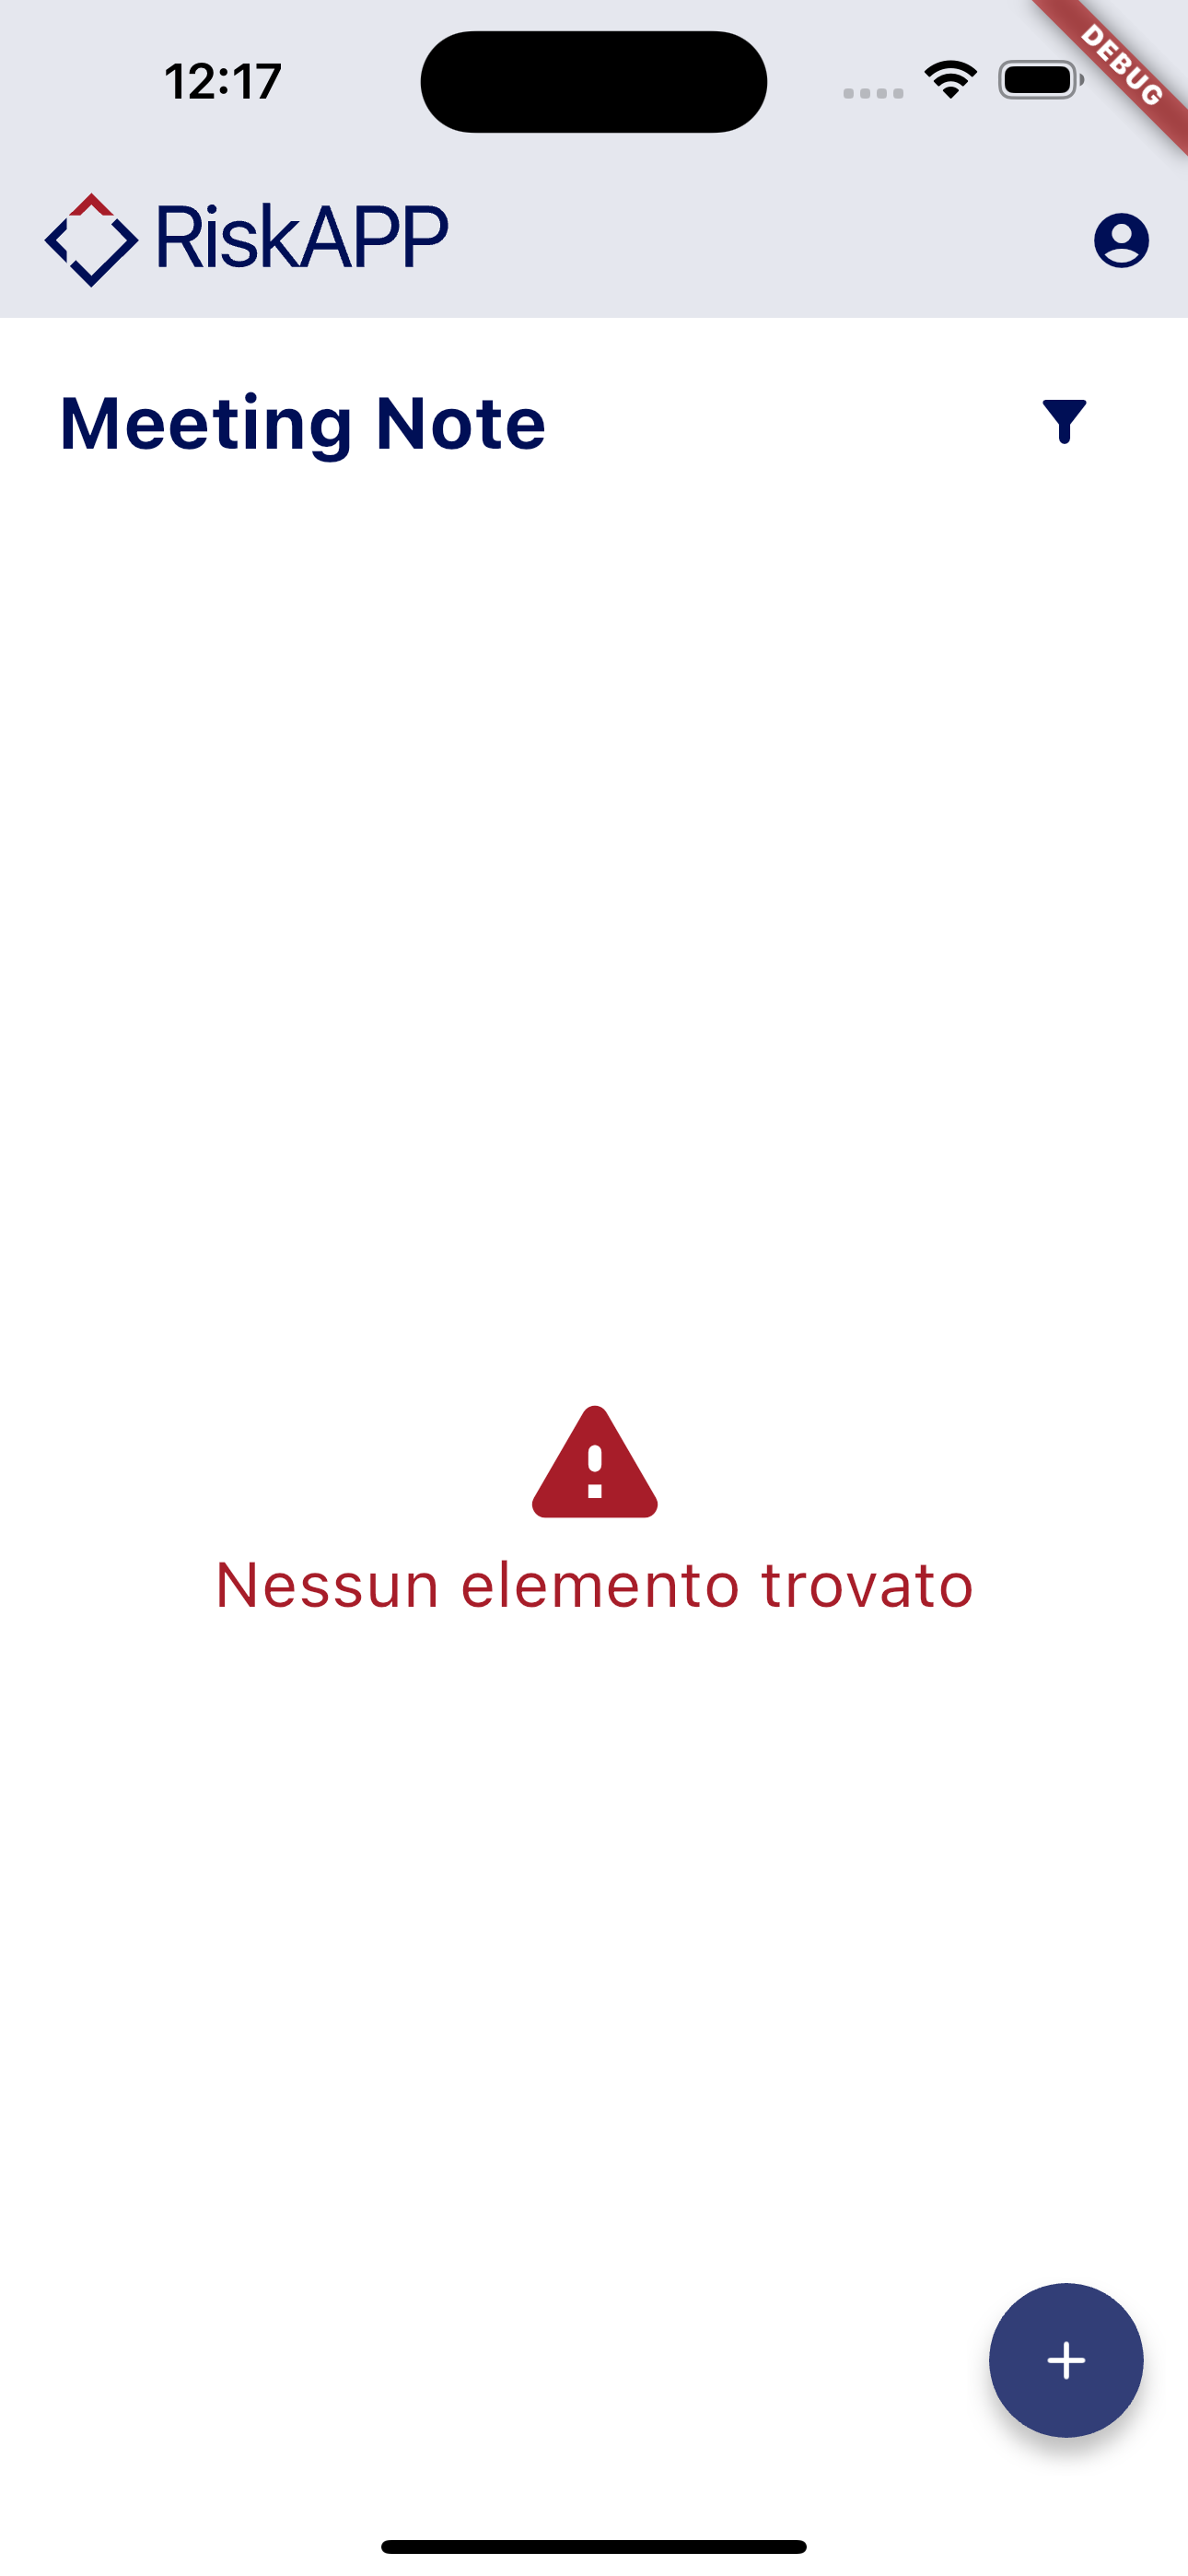
\includegraphics[width=0.3\columnwidth]{screenshot/37-warning_alert1}
    \hfill
    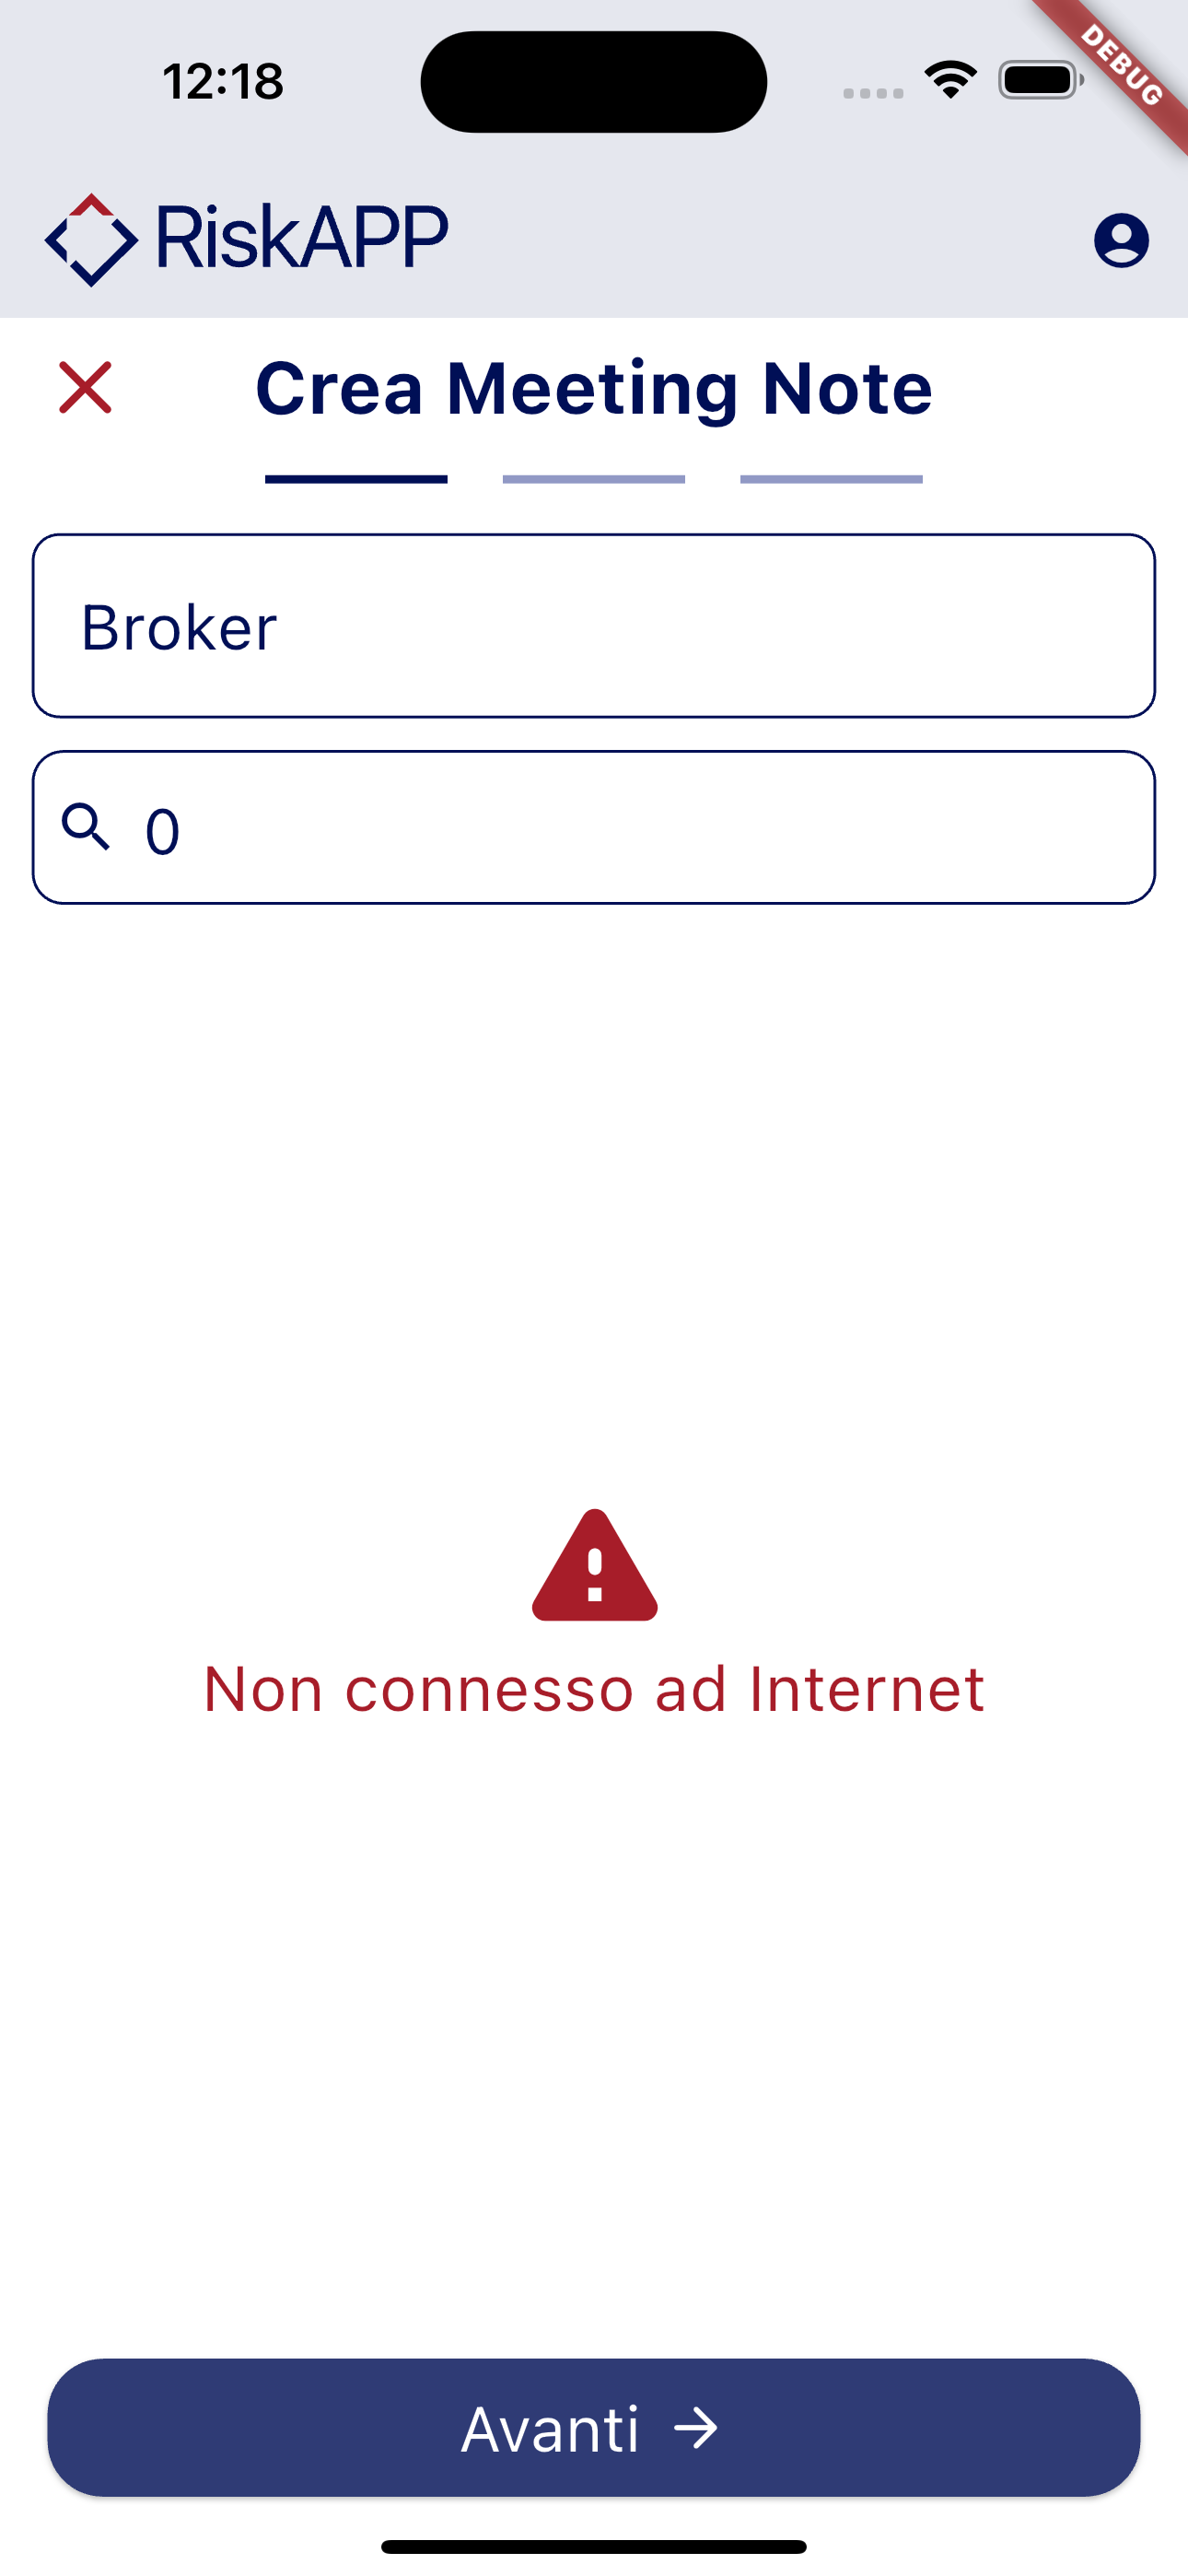
\includegraphics[width=0.3\columnwidth]{screenshot/39-warning_alert3} 
    \caption{Esempio di \emph{WarningAlert}}
    \label{fig:warning-alert}
\end{figure}

\section{Constants}
\label{sec:constants}

In questa cartella sono presenti file che contengono delle costanti utilizzate all'interno dell'applicazione.\\
Le costanti sono incapsulate all'interno di classi, raggrupate in base al loro utilizzo, e sono state definite in maniera statica così da essere richiamate senza dover istanziare un oggetto.\\
Lo scopo è quello di centralizzare tutte le costanti in un unico posto, in modo da poterle modificare facilmente e da poterle utilizzare in maniera uniforme all'interno dell'applicazione.

\subsection{App constants}
\label{subsec:app-constants}

Nel file denominato \lstinline{app_constants.dart} sono state definite delle costanti di tipo \lstinline{String} che rappresentano ad esempio i nomi delle schermate, dei campi di una \emph{Meeting Note} o il contenuto testuale di alcuni pulsanti, ecc.

\subsection{API constants}
\label{subsec:api-constants}

Nel file denominato \lstinline{api_constants.dart} sono state definite due classi che contengono le costanti utilizzate per effettuare le richieste al \gls{backend}\glsoccur.\\
Nella prima classe \lstinline{ApiUrls} sono presenti le costanti che si riferiscono agli \gls{endpoint}\glsoccur dell'\gls{apig}\glsoccur, mentre nella seconda, \lstinline{ApiFields}, sono presenti quelle che si riferiscono al nome dei parametri che devono essere passati all'\gls{urig}\glsoccur di alcune richieste al \gls{backend}\glsoccur. \\
L'utilizzo di queste costanti avviene esclusivamente all'interno delle classi contenute nella cartella \emph{services} (sezione \ref{subsec:services}).

\section{Data}
\label{sec:data}

Questa cartella contiene due cartelle rappresentanti rispettivamente i \emph{data layer} e \emph{domain layer} dell'applicazione.

\subsection{Model}
\label{subsec:model}

Sono contenuti i file che rappresentano il modello dei dati utilizzato all'interno dell'applicazione.\\
Si specifica, per evitare rindondanze, che alcune classi in questione sono state implementate seguendo un \emph{pattern} specifico: oltre alla definizione degli attributi opportuni, ovvero quelli specificati, e che sono vincolanti, nelle \gls{apig}\glsoccur del \gls{backend}\glsoccur, sono presenti un costruttore \emph{factory}\cite{site:factory} \lstinline{fromJson}, come si intuisce si occupa di convertire da \gls{jsong}\glsoccur all'oggetto interessato, dei metodi che ritornano il valore di ciascun attributo e un metodo \lstinline{toString} che ritorna una stringa rappresentante un'istanza della classe.\\
Quest'ultimo metodo è stato definito con il solo scopo di visualizzare il contenuto di un oggetto in fase di \emph{debugging}.
Nel corso di questa sezione verrà specificato quando una classe è stata implementata seguendo tale \emph{pattern}, mentre per le altre verrà descritta nel dettaglio. \\
Inoltre in quasi tutti i file è presente una classe, il cui nome termina con suffisso \lstinline{Response}, che estende \lstinline{BaseResponse} (sezione \ref{subsubsec:status-response}) e rappresenta l'esito di una richiesta \gls{httpg}\glsoccur fatta al \gls{backend}\glsoccur, nel caso in cui l'esito sia positivo contiene anche il valore da restituire.\\
Infine, per ogni classe è sottinteso la presenza del costruttore con tutti gli attributi presenti. 

\subsubsection*{Authentication}
\label{subsubsec:authentication}

In questo file sono state definite tutte le classi necessari per eseguire l'operazione di autenticazione all'applicazione, di seguito verrà descritta l'implementazione di ciascuna.

\paragraph*{AuthArgs} ~ \\
\label{par:auth-args}

\noindent Classe che incapsula i parametri necessari per effettuare la richiesta di autenticazione, è composta da due attributi di tipo \lstinline{String} che rappresentano lo \emph{username} e la \emph{password} dell'utente.\\
Inoltre espone due metodi che si occupano di effettuare degli \gls{overriding}\glsoccur dei metodi \lstinline{operator ==}\cite{site:operator-equals} e \lstinline{hashCode}\cite{site:hascode-property} per poter effettuare il confronto tra due oggetti di tipo \lstinline{AuthArgs}.\\
Infine è presente un metodo \lstinline{toString} che ritorna una stringa rappresentante un'istanza della classe.

\paragraph*{AuthValues} ~ \\
\label{par:auth-values}

\noindent Classe che incapsula il valore restituito dal \gls{backend}\glsoccur in seguito alla richiesta di autenticazione, è composta da un attributo di tipo \lstinline{String} che rappresenta il \emph{token} di autenticazione.\\
La sua implementazione è stata effettuata seguendo il \emph{pattern} descritto nell'introduzione di questa sezione.

\paragraph*{AuthResponse} ~ \\
\label{par:auth-response}

\noindent Classe che estende \lstinline{BaseResponse} (sezione \ref{subsubsec:status-response}), nella quale viene aggiunto un attributo di tipo \lstinline{AuthValues} che ne rappresenta il valore restituito.

\subsubsection*{Meeting Note}
\label{subsubsec:meeting-note}

In questo file sono state definite tutte le classi necessari per gestire i dati riguardanti le \emph{Meeting Note} all'interno dell'applicazione, di seguito verrà descritta l'implementazione di ciascuna.

\paragraph*{RawMeetingNote} ~ \\
\label{par:raw-meeting-note}

\noindent Classe che si occupa di incapsulare i dati di una \emph{Meeting Note} ricevuti da una chiamata al \gls{backend}\glsoccur, che però non sono ancora utilizzabili all'interno dell'applicazione, la quasi totalità degli attributi di tipo \lstinline{String} ed alcuni di essi dunque non sono del tipo opportuno per la loro elaborazione all'interno dell'applicazione.\\
Gli attributi di tipo \lstinline{String} in questione sono:
\begin{itemize}
    \item \lstinline{uuid}, utilizzato per l'identificazione di una \emph{Meeting Note};
    \item \lstinline{meetingDate}, la data dell'incontro;
    \item \lstinline{note}, il contenuto della \emph{Meeting Note};
    \item \lstinline{userCreator}, l'autore della \emph{Meeting Note}.
\end{itemize}
Inoltre sono presenti tre attributi opzionali di tipo \lstinline{MeetingNoteObject}, ciascuno rappresentante un \gls{cliente}\glsoccur delle tre categorie: tra i quali solo uno di loro viene restituito da una chiamata al \emph{backend} e dunque non è nullo, poichè una \emph{Meeting Note} può essere associata ad un solo \gls{cliente}\glsoccur.\\
Una considerazione necessaria da fare è per l'attributo \lstinline{meetingDate} che non è di tipo \lstinline{DateTime}\cite{site:date-time}, dunque non è possibile effettuare ad esempio un confronto tra due date, situazione analoga per l'attributo \lstinline{userCreator} che è di tipo \lstinline{String} e non \lstinline{User}.\\
Per questo motivo è stata definita la classe \lstinline{MeetingNote} (discussa di seguito) che si occupa di effettuare la conversione da \lstinline{RawMeetingNote} a \lstinline{MeetingNote} e permette quindi di operare più facilmente su questi dati. \\
La sua implementazione è stata effettuata seguendo il \emph{pattern} nell'introduzione di questa sezione, con un ulteriore metodo \lstinline{toJson} che si occupa di convertire l'oggetto in \gls{jsong}\glsoccur per poterlo inviare al \gls{backend}\glsoccur.

\paragraph*{PaginatedMeetingNote} ~ \\
\label{par:paginated-meeting-note}

\noindent Classe che si occupa di incapsulare una lista di \lstinline{RawMeetingNote} paginata, con l'ulteriore presenza di due attributi di tipo \lstinline{String} che rappresentano rispettivamente il \emph{link} alla pagina precedente e successiva.\\
La sua implementazione è stata effettuata seguendo il \emph{pattern} nell'introduzione di questa sezione.

\paragraph*{MeetingNote} ~ \\
\label{par:meeting-note}

\noindent Classe che si occupa di incapsulare i dati di una \emph{Meeting Note} pronta per essere utilizzata all'interno dell'applicazione ed è composta dai seguenti attributi:
\begin{itemize}
    \item \lstinline{uuid} di tipo \lstinline{String}, utilizzato per l'identificazione di una \emph{Meeting Note};
    \item \lstinline{meetingDate} di tipo \lstinline{DateTime}\cite{site:date-time}, la data dell'incontro;
    \item \lstinline{note} di tipo \lstinline{String}, il contenuto della \emph{Meeting Note};
    \item \lstinline{user} di tipo \lstinline{User}, l'autore della \emph{Meeting Note};
    \item \lstinline{object} di tipo \lstinline{MeetingNoteObject}, il \gls{cliente}\glsoccur associato alla \emph{Meeting Note}.
\end{itemize}
La sua implementazione, molto semplice, consiste nei metodi per ottenere i valori degli attributi e un metodo \lstinline{toString} che ritorna una stringa che rappresenta l'oggetto.

\paragraph*{MeetingNoteResponse} ~ \\
\label{par:meeting-note-response}

\noindent Classe che estende \lstinline{BaseResponse}, nella quale viene aggiunto un attributo di tipo \lstinline{List<MeetingNote>} che ne rappresenta il valore restituito.

\paragraph*{SmartCreationValue} ~ \\
\label{par:smart-creation-value}

\noindent Classe che si occupa di incapsulare i dati, risultati dell'elaborazione da parte di un algoritmo di \gls{ai}\glsoccur per la creazione automatica di una \emph{Meeting Note}, è composta dai seguenti attributi:
\begin{itemize}
    \item \lstinline{customer} di tipo \lstinline{String}, il nome del \gls{cliente}\glsoccur elaborato dall'algoritmo;
    \item \lstinline{date} di tipo \lstinline{DateTime}, la data dell'incontro elaborato dall'algoritmo;
    \item \lstinline{category} di tipo \lstinline{String}, la categoria del \gls{cliente}\glsoccur elaborato dall'algoritmo;
    \item \lstinline{note} di tipo \lstinline{String}, il contenuto della \emph{Meeting Note} elaborato dall'algoritmo.
\end{itemize}
La sua implementazione è stata effettuata seguendo il \emph{pattern} nell'introduzione di questa sezione, con un ulteriore metodo \lstinline{toJson} che si occupa di convertire l'oggetto in \gls{jsong}\glsoccur per poterlo inviare al \gls{backend}\glsoccur e un altro metodo \lstinline{getObjectCategory} che converte l'attributo \lstinline{category} in un oggetto di tipo \lstinline{ObjectCategory}.

\paragraph*{SmartCreationResponse} ~ \\
\label{par:smart-creation-response}

\noindent Classe che estende \lstinline{BaseResponse}, nella quale viene aggiunto un attributo di tipo \lstinline{SmartCreationValue} che ne rappresenta il valore restituito.

\subsubsection*{Meeting Note Object}
\label{subsubsec:meeting-note-object}

In questo file sono state definite tutte le classi necessarie per gestire i dati riguardanti i \glspl{cliente} all'interno dell'applicazione, di seguito verrà descritta l'implementazione di ciascuna.

\paragraph*{MeetingNoteObject} ~ \\
\label{par:meeting-note-object}

\noindent Classe che rappresenta il modello di un \gls{cliente} relativo ad una \emph{Meeting Note}, ed è composta dai seguenti attributi:
\begin{itemize}
    \item \lstinline{uuid}, di tipo \lstinline{String}, utilizzato per l'identificazione di un \gls{cliente};
    \item \lstinline{name}, di tipo \lstinline{String}, il nome del \gls{cliente};
    \item \lstinline{vatNumber}, di tipo \lstinline{String}, il numero di partita IVA del \gls{cliente} ed è presente solo per i \emph{contraenti};
    \item \lstinline{category}, di tipo \lstinline{ObjectCategory}, la categoria del \gls{cliente}.
\end{itemize}
La sua implementazione è stata effettuata seguendo il \emph{pattern} nell'introduzione di questa sezione.

\paragraph*{PaginatedObject} ~ \\
\label{par:paginated-object}

\noindent Dalle specifiche dell'\gls{apig}\glsoccur, solamente i clienti di tipo \emph{broker} e \emph{contraente} vengono resituiti in modo paginato, per questo motivo è stata definita questa classe che rappresenta un \emph{wrapper} di una lista di \lstinline{MeetingNoteObject} e di due altri attributi di tipo \lstinline{String} che rappresentano rispettivamente il \emph{link} alla pagina precedente e successiva.\\
La sua implementazione è stata effettuata seguendo il \emph{pattern} nell'introduzione di questa sezione.

\paragraph*{ObjectValue} ~ \\
\label{par:object-value}

\noindent É una classe \emph{sealed}\cite{site:sealed-class} in cui è stato definito un costruttore di \emph{default} e un metodo \lstinline{toString} che ritorna una stringa che rappresenta l'oggetto.\\

\paragraph*{ObjectListValue} ~ \\
\label{par:object-list-value}

\noindent Classe che estende \lstinline{ObjectValue} e rappresenta il valore restituito in seguito alla richiesta di ottenere la lista dei clienti, indipendentemente a quale categoria appartengono e se sono paginati o meno.\\
Ridefinisce il costruttore e il metodo \lstinline{toString}, mentre viene aggiunto un metodo per ottenere la lista dei clienti.

\paragraph*{SingleObjectValue} ~ \\
\label{par:single-object-value}

\noindent Classe che estende \lstinline{ObjectValue} e rappresenta il valore restituito in seguito alla richiesta di ottenere un singolo cliente, la sua implementazione è analoga a quella di \lstinline{ObjectListValue}.

\paragraph*{MeetingNoteObjectResponse} ~ \\
\label{par:meeting-note-object-response}

\noindent Classe che estende \lstinline{BaseResponse}, nella quale viene aggiunto un attributo di tipo \lstinline{ObjectValue} che ne rappresenta il valore restituito.

\subsubsection*{Object Category}
\label{subsubsec:object-category}

Si tratta semplicemente di una enumerazione che rappresenta le tre categorie dei \glspl{cliente}\glsoccur:
\begin{itemize}
    \item \lstinline{ObjectCategory.broker}: rappresenta la categoria dei broker;
    \item \lstinline{ObjectCategory.contractor}: rappresenta la categoria dei contraenti;
    \item \lstinline{ObjectCategory.delegatedInsurer}: rappresenta la categoria delle compagnie assicurative.
\end{itemize}

\subsubsection*{Status Response}
\label{subsubsec:status-response}

La classe astratta \lstinline{BaseResponse} modella l'esito di una qualsiasi richiesta \gls{httpg}\glsoccur fatta al \gls{backend}\glsoccur. \\
Ha un attributo di tipo \lstinline{StatusResponse}, una enumerazione che rappresenta tre possibili stati di una richiesta \gls{httpg}\glsoccur:
\begin{itemize}
    \item \lstinline{StatusResponse.success}: la richiesta è andata a buon fine;
    \item \lstinline{StatusResponse.unauthorizedException}: la richiesta non è andata a buon fine a causa del \emph{token} di autenticazione scaduto (sezione \ref{subsec:exception-handler});
    \item \lstinline{StatusResponse.genericException}: la richiesta non è andata a buon fine per un errore generico.
\end{itemize}
Inoltre espone due metodi, il primo si occupa di restituire il valore dell'attributo \lstinline{StatusResponse} e il secondo di restituire una stringa che rappresentante un'istanza della classe.

\subsubsection*{User}
\label{subsubsec:user}

In questo file sono state definite tutte le classi necessari per gestire l'utente all'interno dell'applicazione, di seguito verrà descritta l'implementazione di ciascuna.

\paragraph*{User} ~ \\
\label{par:user}

\noindent Classe che modella l'utente all'interno dell'applicazione, gli attributi che la compongono sono: \emph{email}, \emph{firstName}, \emph{lastName}, di tipo \lstinline{String}, e \emph{profile} di tipo \lstinline{Profile}. \\
La sua implementazione è stata effettuata seguendo il \emph{pattern} specificato nell'introduzione di questa sezione.

\paragraph*{Profile} ~ \\
\label{par:profile}

\noindent Classe che modella il profilo dell'utente all'interno dell'applicazione, gli attributi che la compongono sono: \emph{uuid}, un identificativo univoco assegnato ad ogni utente, e l'\emph{avatar}, contiene il link dell'immagine profilo, entrambi di tipo \lstinline{String}. \\
La sua implementazione è stata effettuata seguendo il \emph{pattern} specificato nell'introduzione di questa sezione.

\paragraph*{UserResponse} ~ \\
\label{par:user-response}

\noindent Classe che estende \lstinline{BaseResponse}, nella quale viene aggiunto un attributo di tipo \lstinline{User} che ne rappresenta il valore restituito.

\subsection{Services}
\label{subsec:services}

In questa sezione verranno discusse le classi che si occupano di effettuare le richieste \gls{httpg}\glsoccur al \gls{backend}\glsoccur attraverso le \gls{apig}\glsoccur, per evitare rindondanze, ogni servizio, eccetto \lstinline{BaseService}, gestisce le eventuali eccezioni in caso una chiamata non vada a buon fine.

\subsubsection*{Authentication Service}
\label{subsubsec:authentication-service}

In questo file è definita una classe che estende \lstinline{BaseService} (classe discussa di seguito) con la composizione di \lstinline{PostRequest} per definire il metodo \lstinline{getToken} che si occupa di effettuare una richiesta \lstinline{POST} al \gls{backend}\glsoccur. \\
Riceve in input un oggetto di tipo \lstinline{AuthArgs} (sezione \ref{subsec:model}) e restituisce un oggetto di tipo \lstinline{AuthResponse}.

\subsubsection*{Base Service}
\label{subsubsec:base-service}

In questo file sono state definite tutte le classi necessarie per fornire un'astrazione per le chiamate \gls{httpg}\glsoccur, di seguito verrà descritta l'implementazione di ciascuna.

\paragraph*{BaseService} ~ \\
\label{par:base-service}

\noindent Classe astratta che si occupa di fornire un'interfaccia per gestire le chiamate \gls{httpg}\glsoccur e provede a definire i metodi fondamentali per effettuare una richiesta:
\begin{itemize}
    \item \lstinline{getUrl}, che si occupa di restituire l'\gls{urig}\glsoccur della risorsa data una stringa in input;
    \item \lstinline{handleResponse}, invocata per ogni tipologia di richiesta, che si occupa di determinare se essa è avvenuta con successo o meno, in caso di quest'ultimo viene lanciata un'eccezione.
\end{itemize}
Le seguenti classi sono di tipo \lstinline{mixin}\cite{site:mixins} e aggiungono funzionalità alla classe \lstinline{BaseService}: ogni classe \lstinline{mixin} si occupa di fornire un implementazione per una chiamata \gls{httpg}\glsoccur specifica. \\
Successivamente, quando verranno utilizzate, la classe in questione dovrà estendere \lstinline{BaseService} e includere alcune di queste classi \lstinline{mixin}, in modo da aggiungere ad un servizio le chiamate necessarie.\\
Di seguito verranno descritte le classi \lstinline{mixin}, per ciascuna si specificheranno i parametri necessari per la configurazione dell'\emph{header} o del \emph{body} della richiesta, a seconda delle necessità. \\

\paragraph*{GetRequest} ~ \\
\label{par:get-request}

\noindent Classe \lstinline{mixin} che si occupa di fornire un'implementazione per effettuare una richiesta \lstinline{GET}, i parametri necessari richiesti nell'\emph{header} sono l'\emph{url} della risorsa e il \emph{token} di autenticazione.

\paragraph*{PatchRequest} ~ \\
\label{par:patch-request}

\noindent Classe \lstinline{mixin} che si occupa di fornire un'implementazione per effettuare una richiesta \lstinline{PATCH}, i parametri necessari sono l'\emph{url} della risorsa, il \emph{token} di autenticazione e il contenuto per il \emph{body} della richiesta.

\paragraph*{DeleteRequest} ~ \\
\label{par:delete-request}

\noindent Classe \lstinline{mixin} che si occupa di fornire un'implementazione per effettuare una richiesta \lstinline{DELETE}, i parametri necessari sono l'\emph{url} della risorsa e il \emph{token} di autenticazione.

\paragraph*{PostRequest} ~ \\
\label{par:post-request}

\noindent Classe \lstinline{mixin} che si occupa di fornire un'implementazione per effettuare una richiesta \lstinline{POST}. \\
Vi sono presenti due metodi, il primo si occupa di effettuare una \lstinline{POST} con lo scopo di salvare dei dati sul \emph{backend}, i parametri necessari sono l'\emph{url} della risorsa, il \emph{token} di autenticazione e il \emph{body} della richiesta. \\
Il secondo si occupa di effettuare una \lstinline{POST} con lo scopo di ottenere il \emph{token} di autenticazione, l'unico parametro necessario è di tipo \lstinline{AuthArgs}.

\subsubsection*{Meeting Note Object Service}
\label{subsubsec:meeting-note-object-service}

In questo file è definita una classe che estende \lstinline{BaseService} (classe discussa in precedenza) con la composizione di \lstinline{GetRequest} per definire i seguenti metodi:
\begin{itemize}
    \item \lstinline{getMeetingNoteObject}, ritorna \lstinline{MeetingNoteObjectResponse} (sezione \ref{subsec:model}) in seguito alla richiesta di ottenere un singolo \gls{cliente}\glsoccur per la creazione di una \emph{Meeting Note}, per fare ciò è necessario passare il \emph{token} di autenticazione, l'\emph{url} della risorsa, includendo il parametro \emph{uuid} del cliente e la sua categoria;
    \item \lstinline{getContractors}, ritorna \lstinline{MeetingNoteObjectResponse} (sezione \ref{subsec:model}) in seguito alla richiesta di ottenere la lista paginata dei \glspl{cliente}\glsoccur di tipo \emph{contraente}, per fare ciò è necessario passare obbligatoriamente il \emph{token} di autenticazione, \lstinline{pageSize} e \lstinline{pageNumber} che rappresentano rispettivamente la dimensione della pagina e il numero della pagina, opzionalmente è possibile passare anche il nome del \gls{cliente} da ricercare;
    \item \lstinline{getBrokers}, implementazione analoga a \lstinline{getContractors} ma per i \glspl{cliente}\glsoccur di tipo \emph{broker};
    \item \lstinline{getDelegatedInsurers}, ritorna \lstinline{MeetingNoteObjectResponse} (sezione \ref{subsec:model}) in seguito alla richiesta di ottenere la lista non paginata dei \glspl{cliente}\glsoccur di una \emph{compagnia assicurativa}, per fare ciò è necessario passare il \emph{token} di autenticazione ed opzionalmente il nome del \gls{cliente} da ricercare;
    \item \lstinline{buildUrl}, si occupa di costruire l'\gls{urig}\glsoccur della risorsa in base ai parametri passati, che sono: l'\emph{url} della risorsa, la dimensione della pagina, il numero della pagina e il nome del \gls{cliente} da ricercare, esso viene utilizzato dai metodi \lstinline{getContractors} e \lstinline{getBrokers}.
\end{itemize}

\subsubsection*{Meeting Note Service}
\label{subsubsec:meeting-note-service}

In questo file è definita una classe che estende \lstinline{BaseService} (classe discussa in precedenza) con la composizione di \lstinline{GetRequest}, \lstinline{PostRequest}, \lstinline{PatchRequest} e \lstinline{DeleteRequest} per definire i seguenti metodi:
\begin{itemize}
    \item \lstinline{getMeetingNotes}, ritorna \lstinline{MeetingNoteResponse} (sezione \ref{subsec:model}) in seguito alla richiesta di ottenere la lista paginata delle \emph{Meeting Note}, per fare ciò è necessario passare obbligatoriamente il \emph{token} di autenticazione, \lstinline{pageSize} e \lstinline{pageNumber} che rappresentano rispettivamente la dimensione della pagina e il numero della pagina, opzionalmente è possibile passare anche un oggetto \lstinline{FilteringOptions} (sezione \ref{subsec:filtering}) che rappresenta le opzioni di filtraggio. \\
    Nel dettaglio, ad ogni chiamata riceve la lista di \lstinline{RawMeetingNote} e la converte in una lista di \lstinline{MeetingNote} (sezione \ref{subsec:model});
    \item \lstinline{postMeetingNote}, ritorna \lstinline{StatusResponse} in seguito alla richiesta di creare una \emph{Meeting Note}, per fare ciò è necessario passare il \emph{token} di autenticazione e un oggetto di tipo \lstinline{MeetingNote} (sezione \ref{subsec:model}), convertendo quest'ultimo in \gls{jsong}\glsoccur attraverso un metodo dedicato;
    \item \lstinline{patchMeetingNote}, ritorna \lstinline{StatusResponse} in seguito alla richiesta di modificare una \emph{Meeting Note}, per fare ciò è necessario passare il \emph{token} di autenticazione e un oggetto di tipo \lstinline{MeetingNote} (sezione \ref{subsec:model}), convertendo quest'ultimo in \gls{jsong}\glsoccur attraverso un metodo dedicato;
    \item \lstinline{deleteMeetingNote}, ritorna \lstinline{StatusResponse} in seguito alla richiesta di eliminare una \emph{Meeting Note}, per fare ciò è necessario passare il \emph{token} di autenticazione e l'\emph{uuid} della \emph{Meeting Note};
    \item \lstinline{postSmartCreationMeetingNote}, ritorna \lstinline{SmartCreationResponse} (sezione \ref{subsec:model}) in seguito alla richiesta di creare una \emph{Meeting Note} in modo automatico, per fare ciò è necessario passare il \emph{token} di autenticazione e il testo da elaborare;;
    \item \lstinline{buildUrl}, si occupa di costruire l'\gls{urig}\glsoccur della risorsa in base ai parametri passati, che sono: la dimensione della pagina, il numero della pagina ed eventualmente le opzioni di filtraggio, esso viene utilizzato dal metodo \lstinline{getMeetingNotes}.
\end{itemize}

\subsubsection*{User Service}
\label{subsubsec:user-service}

In questo file è definita una classe che estende \lstinline{BaseService} (classe discussa in precedenza) con la composizione di \lstinline{GetRequest} per definire il metodo \lstinline{getUser} che si occupa di effettuare una richiesta \lstinline{GET} al \gls{backend}\glsoccur per ottenere i dati dell'utente, ricevendo in input il \emph{token} di autenticazione e tornando un oggetto di tipo \lstinline{UserResponse}.

\section{Provider}
\label{sec:provider}

In questa cartella sono presenti le classi che si occupano di gestire la \emph{logica di business} dell'applicazione, si tratta dunque dell'\emph{application layer} (sezione \ref{subsec:architettura-app}).\\
In ciascun file viene definita una classe al cui interno sono stati implementati dei metodi opportuni per effettuare delle operazioni e al di fuori di essa si istanzia un \lstinline{FutureProvider}\cite{site:future-provider} (discusso nella sezione \ref{subsec:riverpod}) per esporre questi metodi al \emph{presentation layer}.\\
Inoltre ciascuna classe per effettuare le operazioni necessarie si avvale dei corrispettivi servizi (sezione \ref{subsec:services}) e modelli (sezione \ref{subsec:model}) precedentemente discussi. \\
Si vuole infine precisare che, eccetto per \lstinline{AuthenticationHelper} (sezione \ref{subsec:authentication-provider}), nelle restanti classi, ogni metodo che effettua una richiesta include l'operazione di lettura del \emph{token} per autenticare quest'ultime.

\subsection{Authentication Provider}
\label{subsec:authentication-provider}

In questo file è definita la classe \lstinline{AuthenticationHelper} che si occupa di gestire la logica dell'autenticazione all'applicazione, in particolare espone i seguenti metodi:
\begin{itemize}
    \item \lstinline{verifyCredentials}, si occupa di verificare la validità delle credenziali, passate per parametro, inserite dall'utente;
    \item \lstinline{authenticate}, verifica le credenziali dell'utente, avvalendosi del metodo \lstinline{verifyCredentials} e in caso di successo ritorna un \emph{token} di autenticazione attraverso l'oggetto \lstinline{AuthResponse} salvandolo poi in locale con l'ausilio della libreria \lstinline{shared_preferences}\cite{site:shared-preferences} (sezione \ref{subsec:shared-preferences});
    \item \lstinline{logout}, si occupa di effettuare il \emph{logout} dall'applicazione, eliminando il \emph{token} di autenticazione salvato in locale e riportando l'utente alla schermata di \emph{login};
    \item \lstinline{isAuthenticated}, verifica se l'utente è autenticato, controllando se il \emph{token} di autenticazione è salvato in locale;
    \item \lstinline{isUnauthorized}, verifica se l'utente è autorizzato ad effettuare una chiamata \gls{httpg}\glsoccur, controllandone l'esito e in caso negativo effettua il \emph{logout} dall'applicazione, poichè significa che il \emph{token} di autenticazione è scaduto;
    \item \lstinline{isBiometricEnabled}, verifica se l'utente ha abilitato l'autenticazione biometrica all'interno dell'applicazione, controllando se il \emph{flag} è salvato in locale;
    \item \lstinline{readCredentials}, si occupa di leggere le credenziali cifrate salvate in locale, attraverso la libreria \lstinline{FlutterSecureStorage}\cite{site:flutter-secure-storage}, restituendo un oggetto di tipo \lstinline{AuthArgs} (sezione \ref{subsec:model});
    \item \lstinline{saveCredentials}, si occupa di salvare le credenziali cifrate in locale, ricevendo in input un oggetto di tipo \lstinline{AuthArgs} (sezione \ref{subsec:model});
    \item \lstinline{removeCredentials}, si occupa di eliminare le credenziali cifrate salvate in locale;
\end{itemize}

\subsection{Meeting Note Object Provider}
\label{subsec:meeting-note-object-provider}

In questo file è definita la classe \lstinline{MeetingNoteObjectHelper} che si occupa di gestire la logica dei \glspl{cliente}\glsoccur all'interno dell'applicazione, in particolare espone i seguenti metodi:
\begin{itemize}
    \item \lstinline{getContractors} si occupa di ottenere la lista paginata di tutti i \glspl{cliente}\glsoccur di tipo \emph{contraente} oppure solo di quelli ricercati dall'utente attraverso il passaggio del parametro \lstinline{searchTerm}, dati in input il numero della pagina e la dimensione della pagina, restituendo un oggetto di tipo \lstinline{MeetingNoteObjectResponse};
    \item \lstinline{getBrokers} implementazione analoga a \lstinline{getContractors} ma per i \glspl{cliente}\glsoccur di tipo \emph{broker};
    \item \lstinline{getDelegatedInsurers} implementazione analoga ai due metodi precedenti ma per i \glspl{cliente}\glsoccur di tipo \emph{compagnia assicurativa} e senza la possibilità di paginazione.
\end{itemize}

\subsection{Meeting Note Provider}
\label{subsec:meeting-note-provider}

In questo file è definita la classe \lstinline{MeetingNoteHelper} che si occupa di gestire la logica delle \emph{Meeting Note} all'interno dell'applicazione, in particolare espone i seguenti metodi:
\begin{itemize}
    \item \lstinline{fecthMeetingNotes}, si occupa di ottenere la lista paginata delle \emph{Meeting Note} oppure solo di quelle filtrate dall'utente attraverso il passaggio del parametro \lstinline{filteringOptions} (sezione \ref{subsec:filtering}), dati in input il numero della pagina e la dimensione della pagina, restituendo un oggetto di tipo \lstinline{MeetingNoteResponse};
    \item \lstinline{createMeetingNote}, si occupa di memorizzare la \emph{Meeting Note} creata e passata in input come oggetto di tipo \lstinline{MeetingNote} nel \gls{backend}\glsoccur, restituendo un oggetto di tipo \lstinline{StatusResponse} in quanto è sufficiente ritornare l'esito della richiesta;
    \item \lstinline{deleteMeetingNote}, si occupa di eliminare la \emph{Meeting Note} passata in input lo \lstinline{uuid} come parametro, restituendo un oggetto di tipo \lstinline{StatusResponse} in quanto è sufficiente ritornare l'esito della richiesta;
    \item \lstinline{modifyMeetingNote}, si occupa di modificare la \emph{Meeting Note} passata in input come oggetto di tipo \lstinline{MeetingNote}, restituendo un oggetto di tipo \lstinline{StatusResponse} in quanto è sufficiente ritornare l'esito della richiesta;
    \item \lstinline{smartCreation}, si occupa di creare una \emph{Meeting Note} in modo automatico, passando in input il testo da elaborare, restituendo un oggetto di tipo \lstinline{SmartCreationResponse}.
\end{itemize}

\subsection{User Provider}
\label{subsec:user-provider}

In questo file è definita la classe \lstinline{UserHelper} che si occupa di gestire la logica dell'utente all'interno dell'applicazione, in particolare espone il metodo \lstinline{initUser} che si occupa di ottenere i dati dell'utente, restituendo un oggetto di tipo \lstinline{UserResponse}.

\section{Screens}
\label{sec:screens}

In questa cartella sono presenti tutte le schermate dell'applicazione, le quali verranno descritte di seguito.

\subsection{Account Screen}
\label{subsec:account-screen}

Schermata che permette all'utente di visualizzare i propri dati, letti attraverso \lstinline{UserProvider} (sezione \ref{subsec:user-provider}), la cui classe estende \lstinline{ConsumerWidget} (sezione \ref{subsec:riverpod}) in modo da essere in grado di invocare un \emph{provider}. \\
Per la definizione dell'aspetto grafico questa schermata implementa \lstinline{BaseScreen} (sezione \ref{subsec:screens-template}) e prima di renderizzare ulteriori componenti effettua un controllo sullo stato della connessione ad internet, ottenuto attraverso il \lstinline{NetworkAwareProvider} (sezione \ref{subsec:network-handler}), in caso di assenza di connessione viene mostrato un \lstinline{WarningAlert} (sezione \ref{subsec:warning-alert}) con il relativo messaggio di errore. \\
Altrimenti viene mostrato il contenuto della schermata servendosi di \lstinline{FutureBuilder}\cite{site:future-builder} per invocare il metodo \lstinline{initUser} e ottenere i dati dell'utente, in particolare ci possono essere vari esiti:
\begin{itemize}
    \item \emph{waiting}, viene mostrato un \lstinline{CircularProgressIndicator}\cite{site:circular-progress-indicator} per indicare che la richiesta è in corso;
    \item \emph{unauthorizedException}, l'utente non è autorizzato ad effettuare la richiesta, viene reindirizzato alla schermata di \emph{login};
    \item \emph{genericException}, la richiesta non è andata a buon fine per un errore generico e viene mostrato un \lstinline{WarningAlert} con il relativo messaggio di errore;
    \item \emph{success}, la richiesta è andata a buon fine e viene mostrato il contenuto della schermata.
\end{itemize}
In quest'ultimo caso vengono renderizzati i seguenti componenti (figura \ref{fig:account-screen}):
\begin{itemize}
    \item \lstinline{TextButton}\cite{site:text-button}, effettua il \emph{logout} dall'applicazione, alla sua pressione mostra un \lstinline{WarningAlertDialog} (sezione \ref{subsec:warning-alert}) informando l'utente dell'evento, che ne deve confermare o meno l'operazione;
    \item \lstinline{CircleAvatar}\cite{site:circle-avatar}, mostra l'immagine profilo dell'utente;
    \item \lstinline{AccountCard}, \emph{StatelessWidget} privato, creato appositamente con lo scopo di definire l'aspetto grafico per la visualizzazione del nome, cognome e la mail dell'utente;
    \item \lstinline{BiometricOption}, \emph{StatefulWidget} privato che implementa \lstinline{BiometricSwitch} (sezione \ref{subsec:biometric-switch}), si ricorda che lo stato di questo componente è salvato in locale attraverso la libreria \lstinline{shared_preferences}\cite{site:shared-preferences} (sezione \ref{subsec:shared-preferences}); per la sua attivazione verrà richiesto all'utente di confermare l'operazione attraverso l'inserimento delle credenziali di autenticazione, anch'esse salvate in locale attraverso la libreria \lstinline{FlutterSecureStorage}\cite{site:flutter-secure-storage} (sezione \ref{subsec:shared-preferences}).
\end{itemize}

\begin{figure}[!h] 
    \centering 
    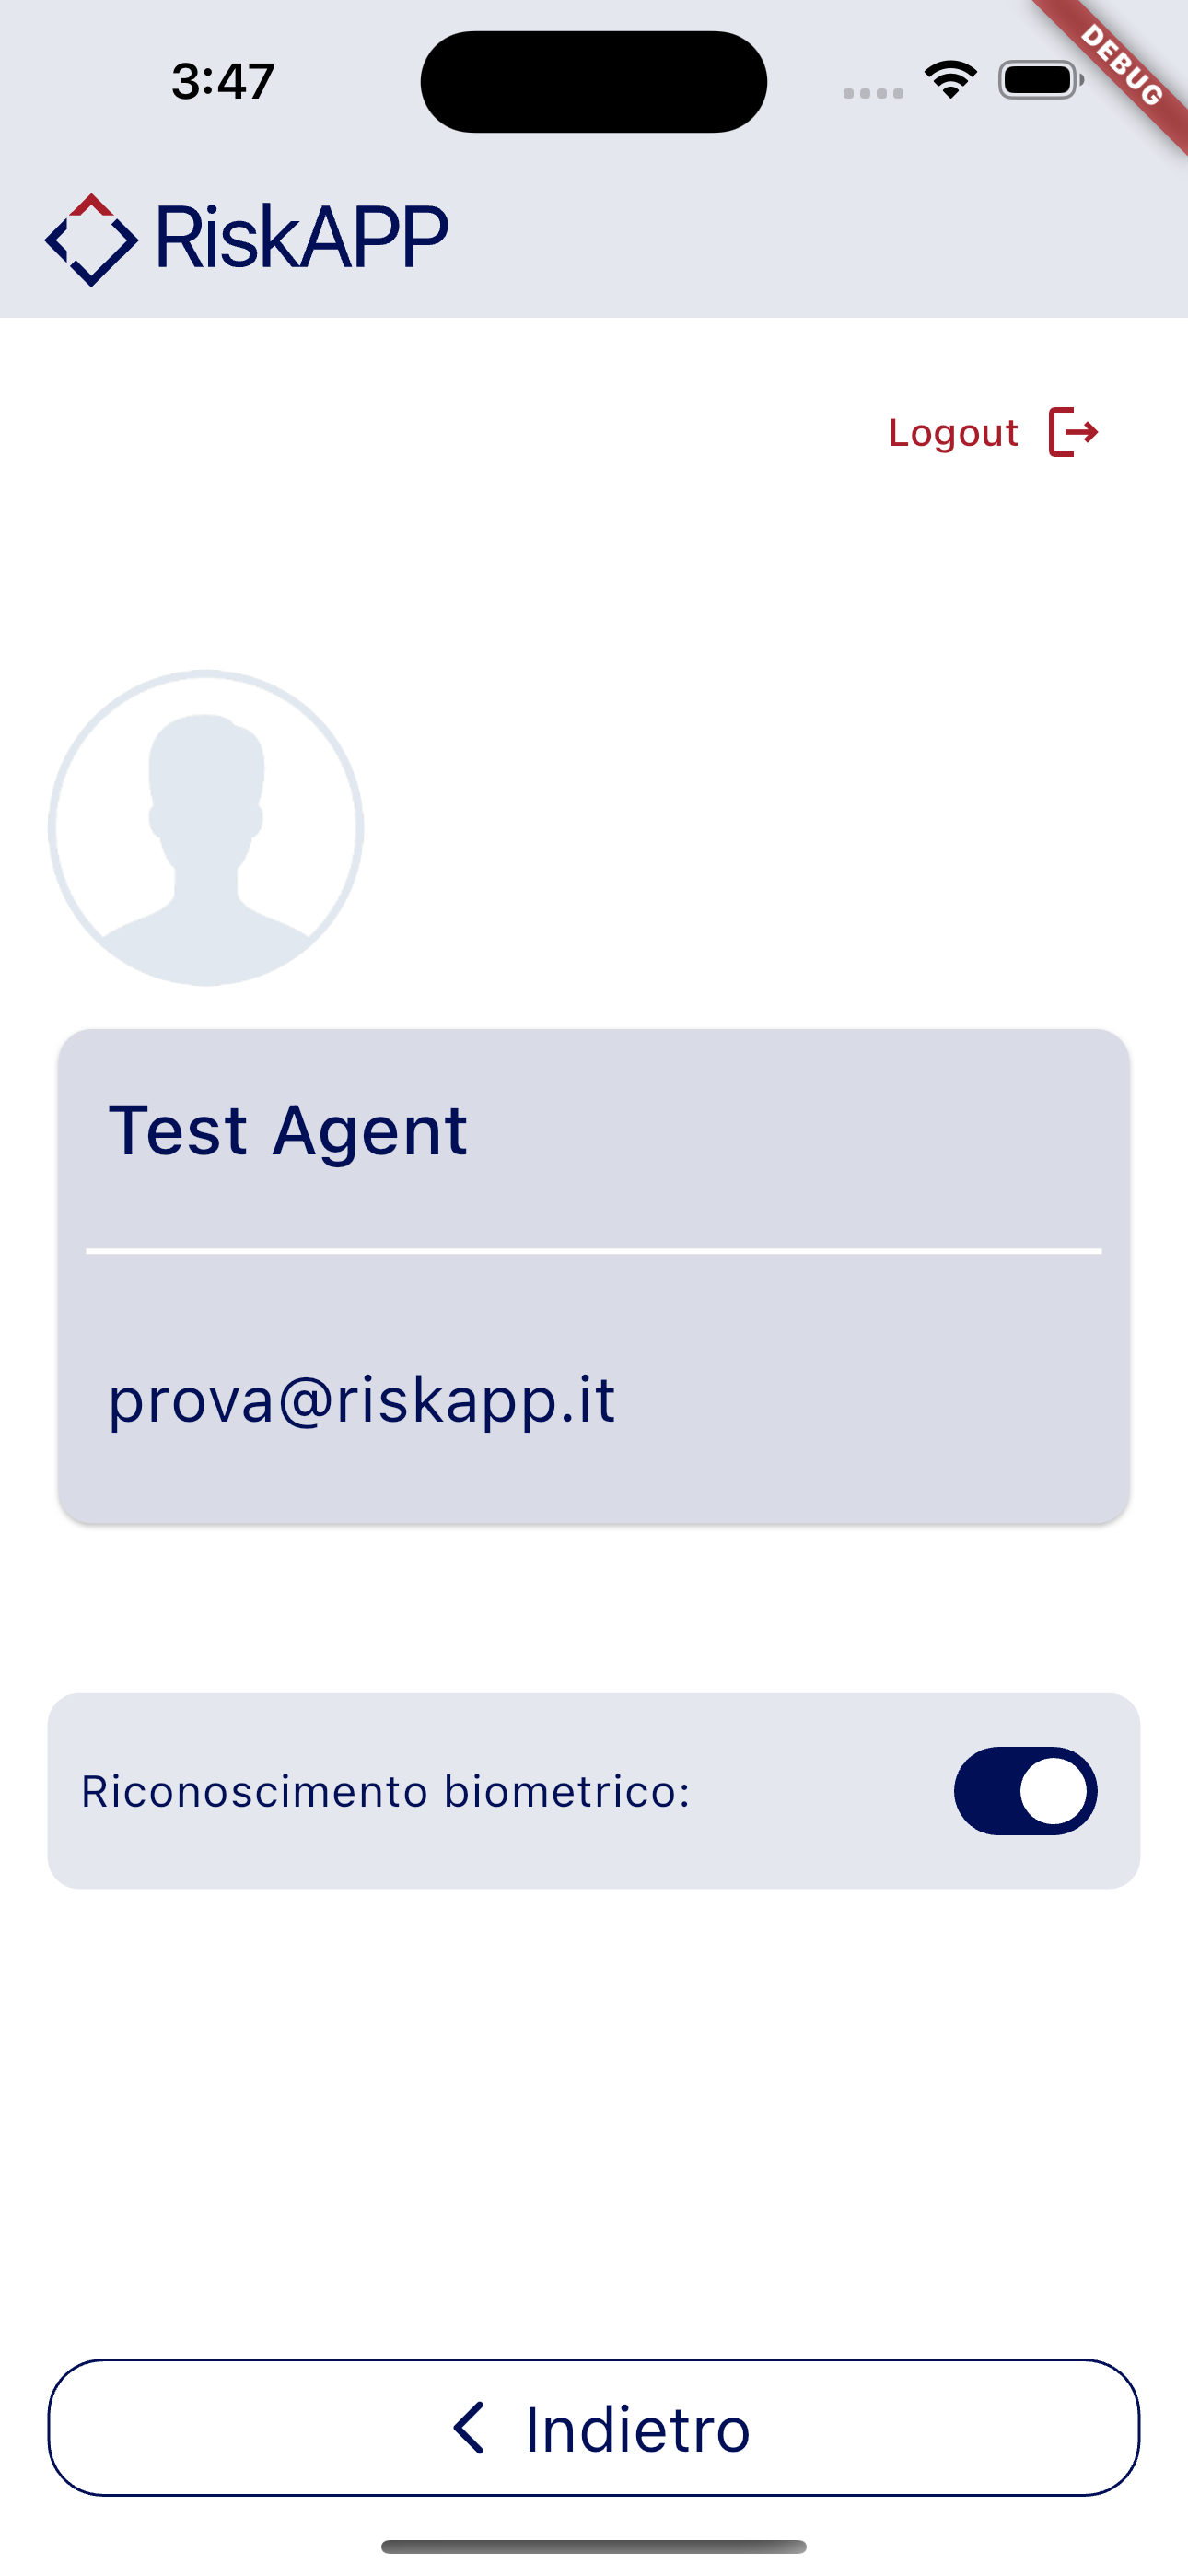
\includegraphics[width=0.3\columnwidth]{screenshot/6-account_screen} 
    \caption{Account Screen}
    \label{fig:account-screen}
\end{figure}

\subsection{Home Screen}
\label{subsec:home-screen}

Schermata principale dell'applicazione, la cui classe estende \lstinline{ConsumerStatefulWidget} (sezione \ref{subsec:riverpod}) in modo da essere in grado di invocare un \emph{provider}. \\
Prima della renderizzazione dell'aspetto grafico viene effettuata l'inizializzazione delle variabili di stato, in particolare:
\begin{itemize}
    \item \lstinline{filteringOptions}, oggetto di tipo \lstinline{FilteringOptions} (sezione \ref{subsec:filtering}) che incapsula le opzioni di filtraggio attive;
    \item \lstinline{isFiltering}, \lstinline{bool} che indica se l'utente ha attivato o meno almeno un filtro;
    \item \lstinline{pagingController}, oggetto di tipo \lstinline{PagingController}\cite{site:infinite-scroll-pagination} che si occupa di gestire la paginazione dei dati.
\end{itemize}
Per la definizione dell'aspetto grafico questa schermata implementa \lstinline{BaseScreen} (sezione \ref{subsec:screens-template}) e il suo contenuto è strutturato come segue (figura \ref{fig:home-screen}):
\begin{itemize}
    \item \lstinline{HomeHeader}, \emph{StatelessWidget} privato che mostra il titolo della schermata e due pulsanti, uno per eliminare i filtri attivati e l'altro per aprire il \lstinline{FilterPanel} (sezione \ref{subsec:filter-panel});
    \item \lstinline{SpeedDial}, componente che mostra un \lstinline{FloatingActionButton}\cite{site:fab} che consente all'utente di scegliere la modalità di creazione di una \emph{Meeting Note}, in base alla scelta quest'ultimo verrà reindirizzato alla schermata corrispondente;
    \item \lstinline{PagedListView}\cite{site:infinite-scroll-pagination}, componente che si occupa di mostrare la lista paginata delle \emph{Meeting Note}, in particolare si avvale del \lstinline{PagingController} per gestire la paginazione dei dati, lista che è composta da \lstinline{MeetingNoteItem} (sezione \ref{subsec:meeting-note-card}) che definisce la rappresentazione grafica della \emph{Meeting Note} e permette all'utente di modificarla o eliminarla.
\end{itemize}
Nel dettaglio, prima della visualizzazione della lista paginata, si effettua un controllo dello stato della connessione ad internet attraverso il \lstinline{NetworkAwareProvider} (sezione \ref{subsec:network-handler}), in caso di assenza di connessione viene mostrato un \lstinline{WarningAlert} (sezione \ref{subsec:warning-alert}) con il relativo messaggio di errore. \\
Altrimenti viene mostrato il contenuto della schermata servendosi del metodo privato \lstinline{fetchPage} che si occupa di effettuare la richiesta al \gls{backend}\glsoccur attraverso \lstinline{MeetingNoteProvider} (sezione \ref{subsec:meeting-note-provider}), controllando se l'utente è autorizzato ad effettuare la richiesta attraverso il metodo \lstinline{isUnauthorized} fornito da \lstinline{authProvider} (sezione \ref{subsec:authentication-provider}), per poi restituire la lista paginata delle \emph{Meeting Note} e aggiornare lo stato del \lstinline{PagingController}. \\
È presente un ulteriore metodo privato \lstinline{showWarningDialog} che si occupa di mostrare un \lstinline{WarningAlertDialog} (sezione \ref{subsec:warning-alert}) chiedendo conferma l'utente per la eliminazione di una \emph{Meeting Note} e in base alla scelta dell'utente e all'esito della richiesta, vengono gestiti i seguenti casi {i medesimi illustrati nella sezione \ref{subsec:model}, paragrafo \emph{StatusResponse}}.

\begin{figure}[!h] 
    \centering 
    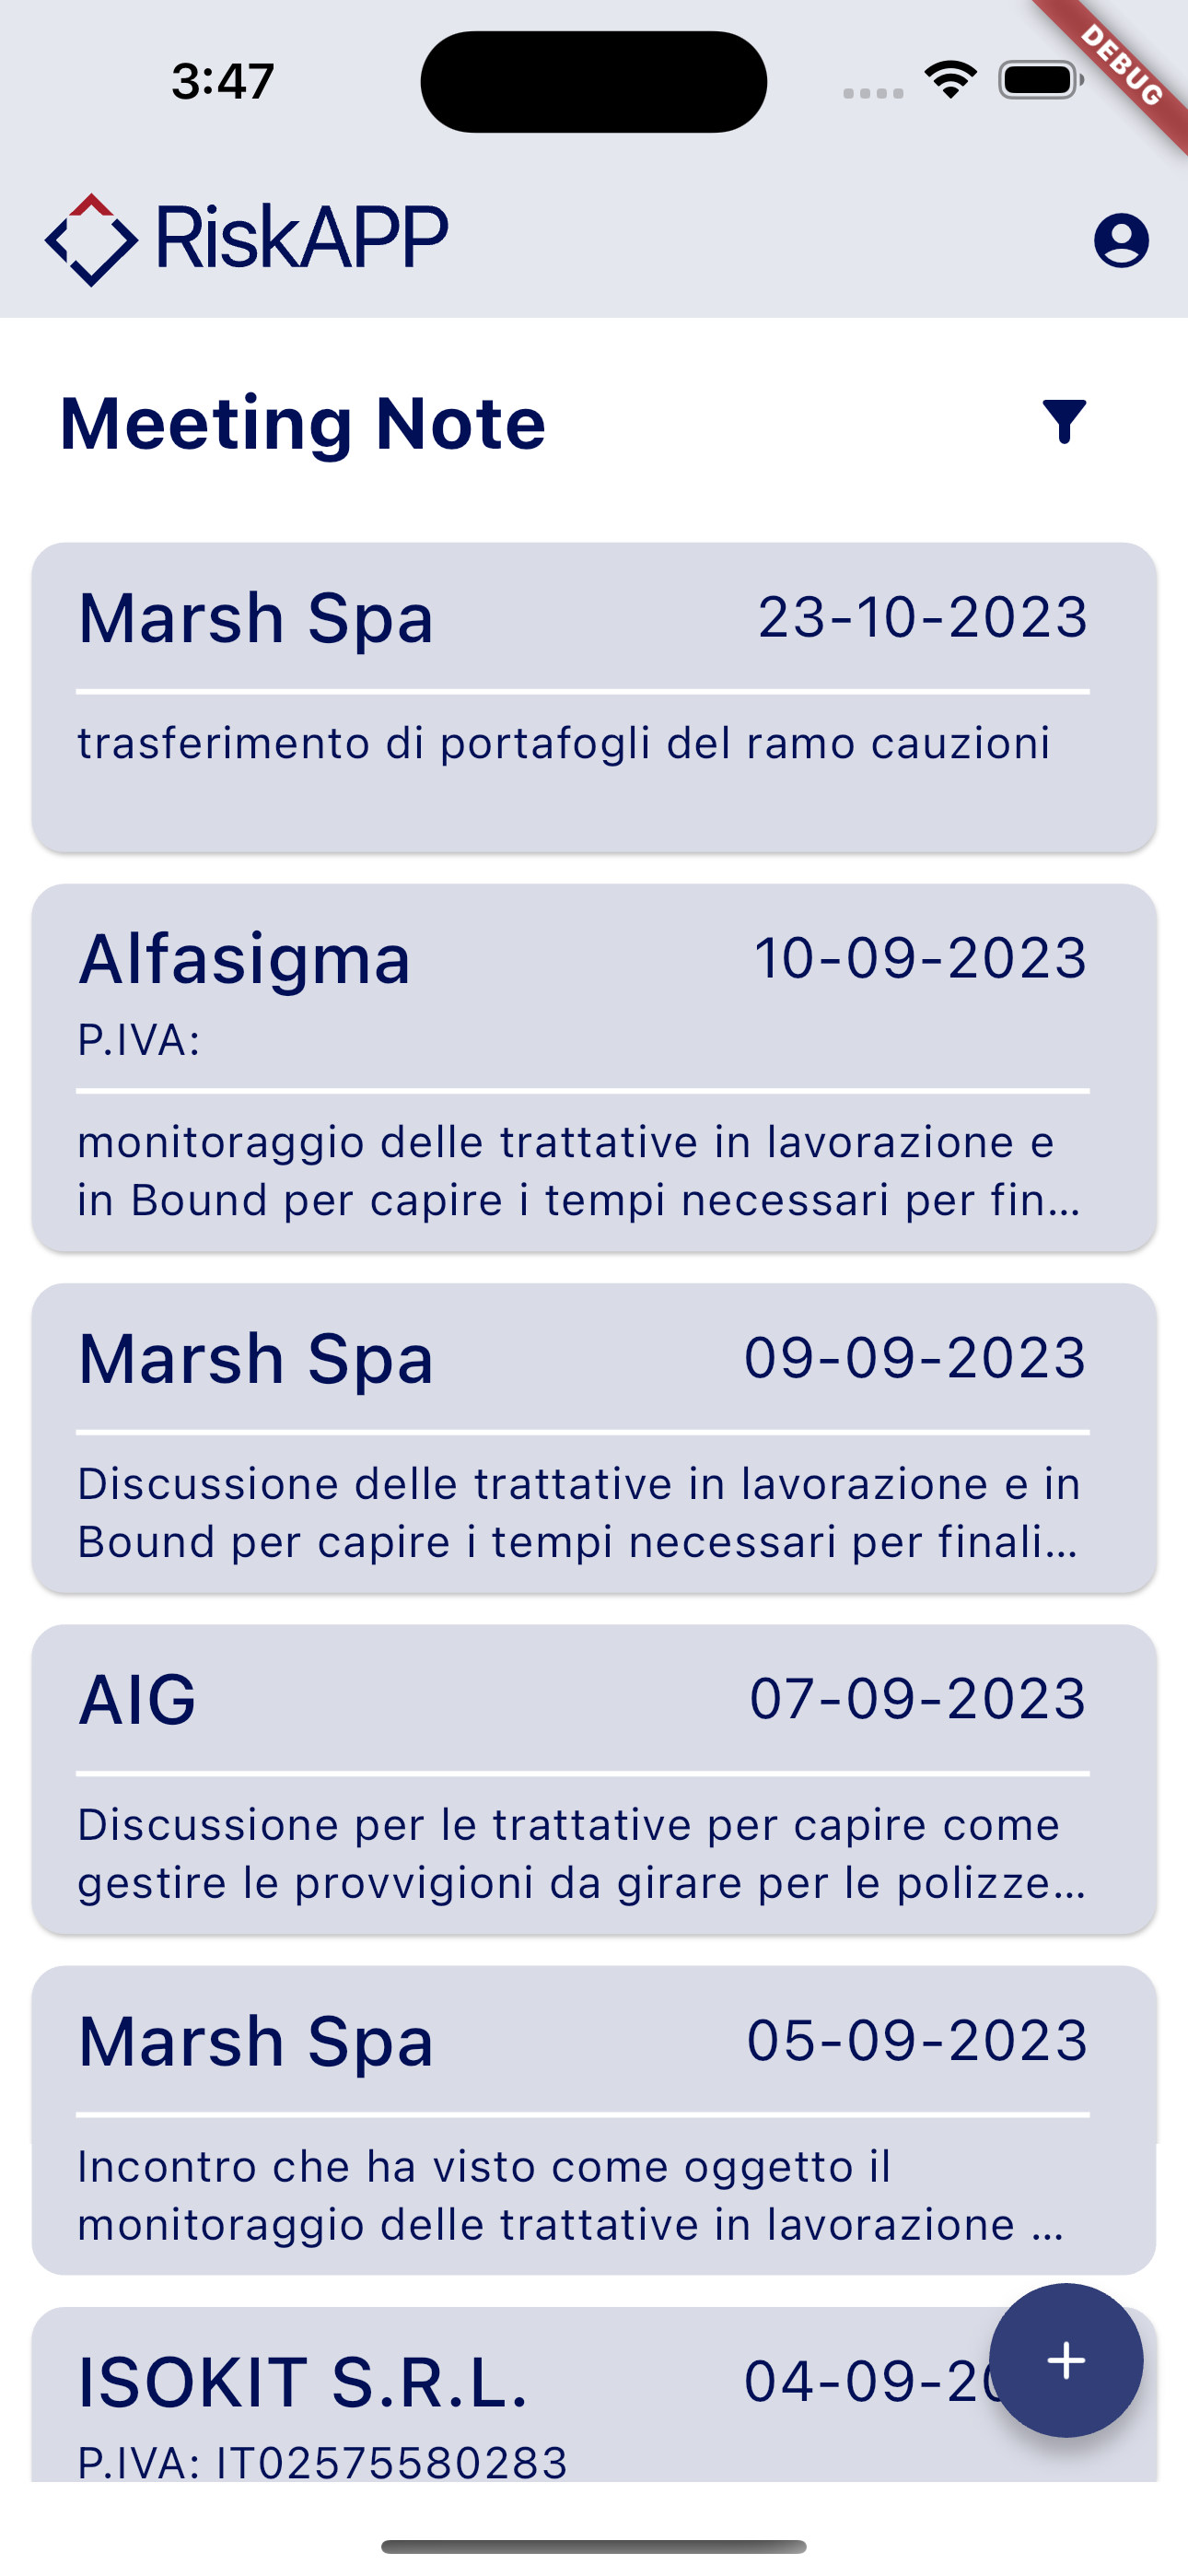
\includegraphics[width=0.3\columnwidth]{screenshot/5-home_screen}
    \caption{Home Screen}
    \label{fig:home-screen}
\end{figure}

\newpage

\subsection{Login Screen}
\label{subsec:login-screen}

Schermata che permette all'utente di effettuare l'autenticazione all'applicazione. \\
Definisce semplicemente l'aspetto grafico della schermata (figura \ref{fig:login-screen}): implementando \lstinline{BaseScreen} (sezione \ref{subsec:screens-template}), impostando \lstinline{LoginAppBar} (sezione \ref{subsec:app-bars}) e nel \lstinline{body} viene definito il titolo e richiamato il \lstinline{LoginForm} (sezione \ref{subsec:login-form}), che si occupa di gestire il comportamento e per questo motivo tale classe viene estesa con \emph{StatelessWidget}.

\begin{figure}[!h] 
    \centering 
    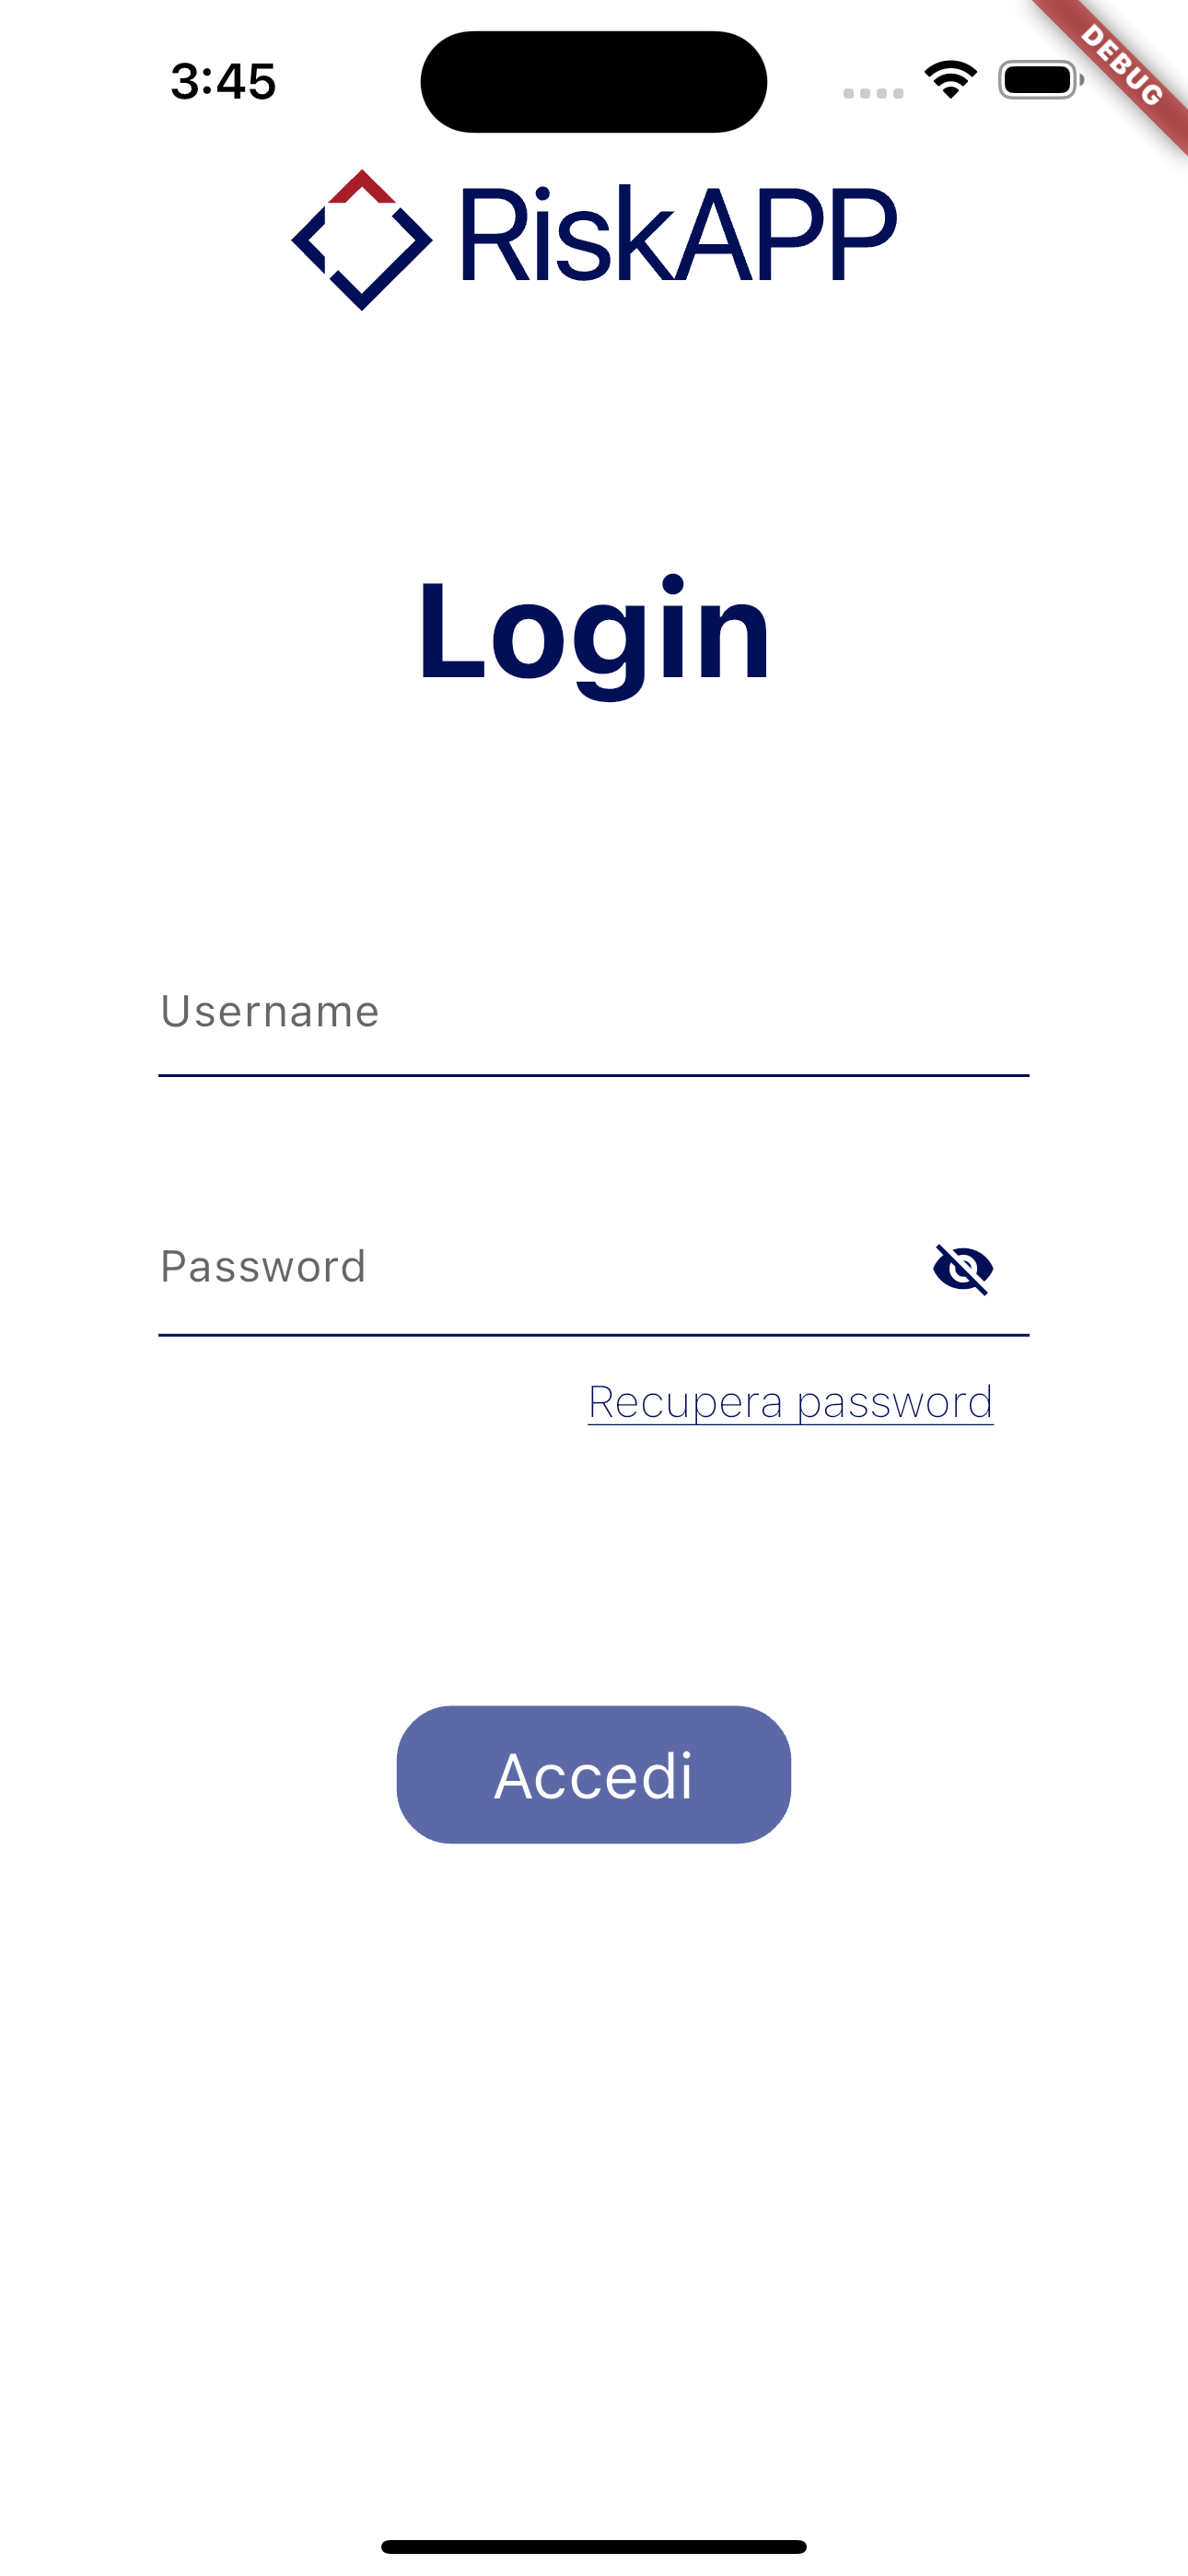
\includegraphics[width=0.3\columnwidth]{screenshot/1-login_screen} 
    \caption{Login Screen}
    \label{fig:login-screen}
\end{figure}

\newpage

\subsection{Smart Creation Screen}
\label{subsec:smart-creation-screen}

Schermata che permette all'utente di creare una \emph{Meeting Note} in modo automatico e data la sua complessità, essa è stata suddivisa in tre classi, di seguito verranno descritte nel dettaglio. \\

\subsubsection*{SmartCreationPage}
\label{subsubsec:smart-creation-page}

Classe che si occupa di ricevere in input il contenuto testuale dall'utente che verrà elaborato da un algoritmo di \emph{intelligenza artificiale} per creare una \emph{Meeting Note} in modo automatico. \\
Prima della renderizzazione dell'aspetto grafico viene effettuata l'inizializzazione delle variabili di stato, in particolare:
\begin{itemize}
    \item \lstinline{textController}, \lstinline{TextEditingController}\cite{site:text-editing-controller} che si occupa di gestire il contenuto testuale inserito dall'utente;
    \item \lstinline{isButtonEnabled}, \lstinline{bool} che indica se l'utente ha inserito del testo oppure no e abilita di conseguenza il pulsante che avvia l'elaborazione del testo;
    \item \lstinline{speechToText}, \lstinline{SpeechToText}\cite{site:speech-to-text} che si occupa di gestire la dettatura vocale;
    \item \lstinline{listenedWords}, \lstinline{String} che memorizza quanto detto dall'utente.
\end{itemize}
Per la definizione dell'aspetto grafico questa schermata implementa \lstinline{WizardScreen} (sezione \ref{subsec:screens-template}) e il suo contenuto è strutturato come segue (figura \ref{fig:smart-screen}):
\begin{itemize}
    \item \lstinline{WizardHeader}, imposta il titolo della schermata (sezione \ref{subsec:screens-template});
    \item \lstinline{CustomTextBox}, componente che si occupa di ricevere in input il contenuto testuale inserito dall'utente, che può avvenire in due modalità differenti come specificato nei requisiti \hyperref[RFN-72]{RFN-72} e \hyperref[RFN-73]{RFN-73} (sezione \ref{subsec:text-box});
    \item \lstinline{RecordingButton}, componente che si occupa attivare la dettatura vocale (sezione \ref{subsec:recording-button});
    \item \lstinline{ElevatedButton}\cite{site:elevated-button}, componente che si occupa di avviare l'elaborazione del testo inserito dall'utente.
\end{itemize}
Nel dettaglio quest'ultima operazione viene effettuata servendosi di \lstinline{meetingNoteProvider} per effettuare l'elaborazione e di \lstinline{authProvider} per autorizzare la richiesta attraverso il metodo \lstinline{isUnauthorized}, inoltre viene mostrato un \lstinline{CircularProgressIndicator}\cite{site:circular-progress-indicator} per indicare che la richiesta è in corso. \\
Al termine dell'elaborazione, con i tre possibili esiti (i medesimi illustrati nella sezione \ref{subsec:model}, paragrafo \emph{Status Response}), e in caso di successo viene mostrato \lstinline{ConfirmCreationPopup} attraverso una modale che appare dal basso.

\begin{figure}[!h] 
    \centering 
    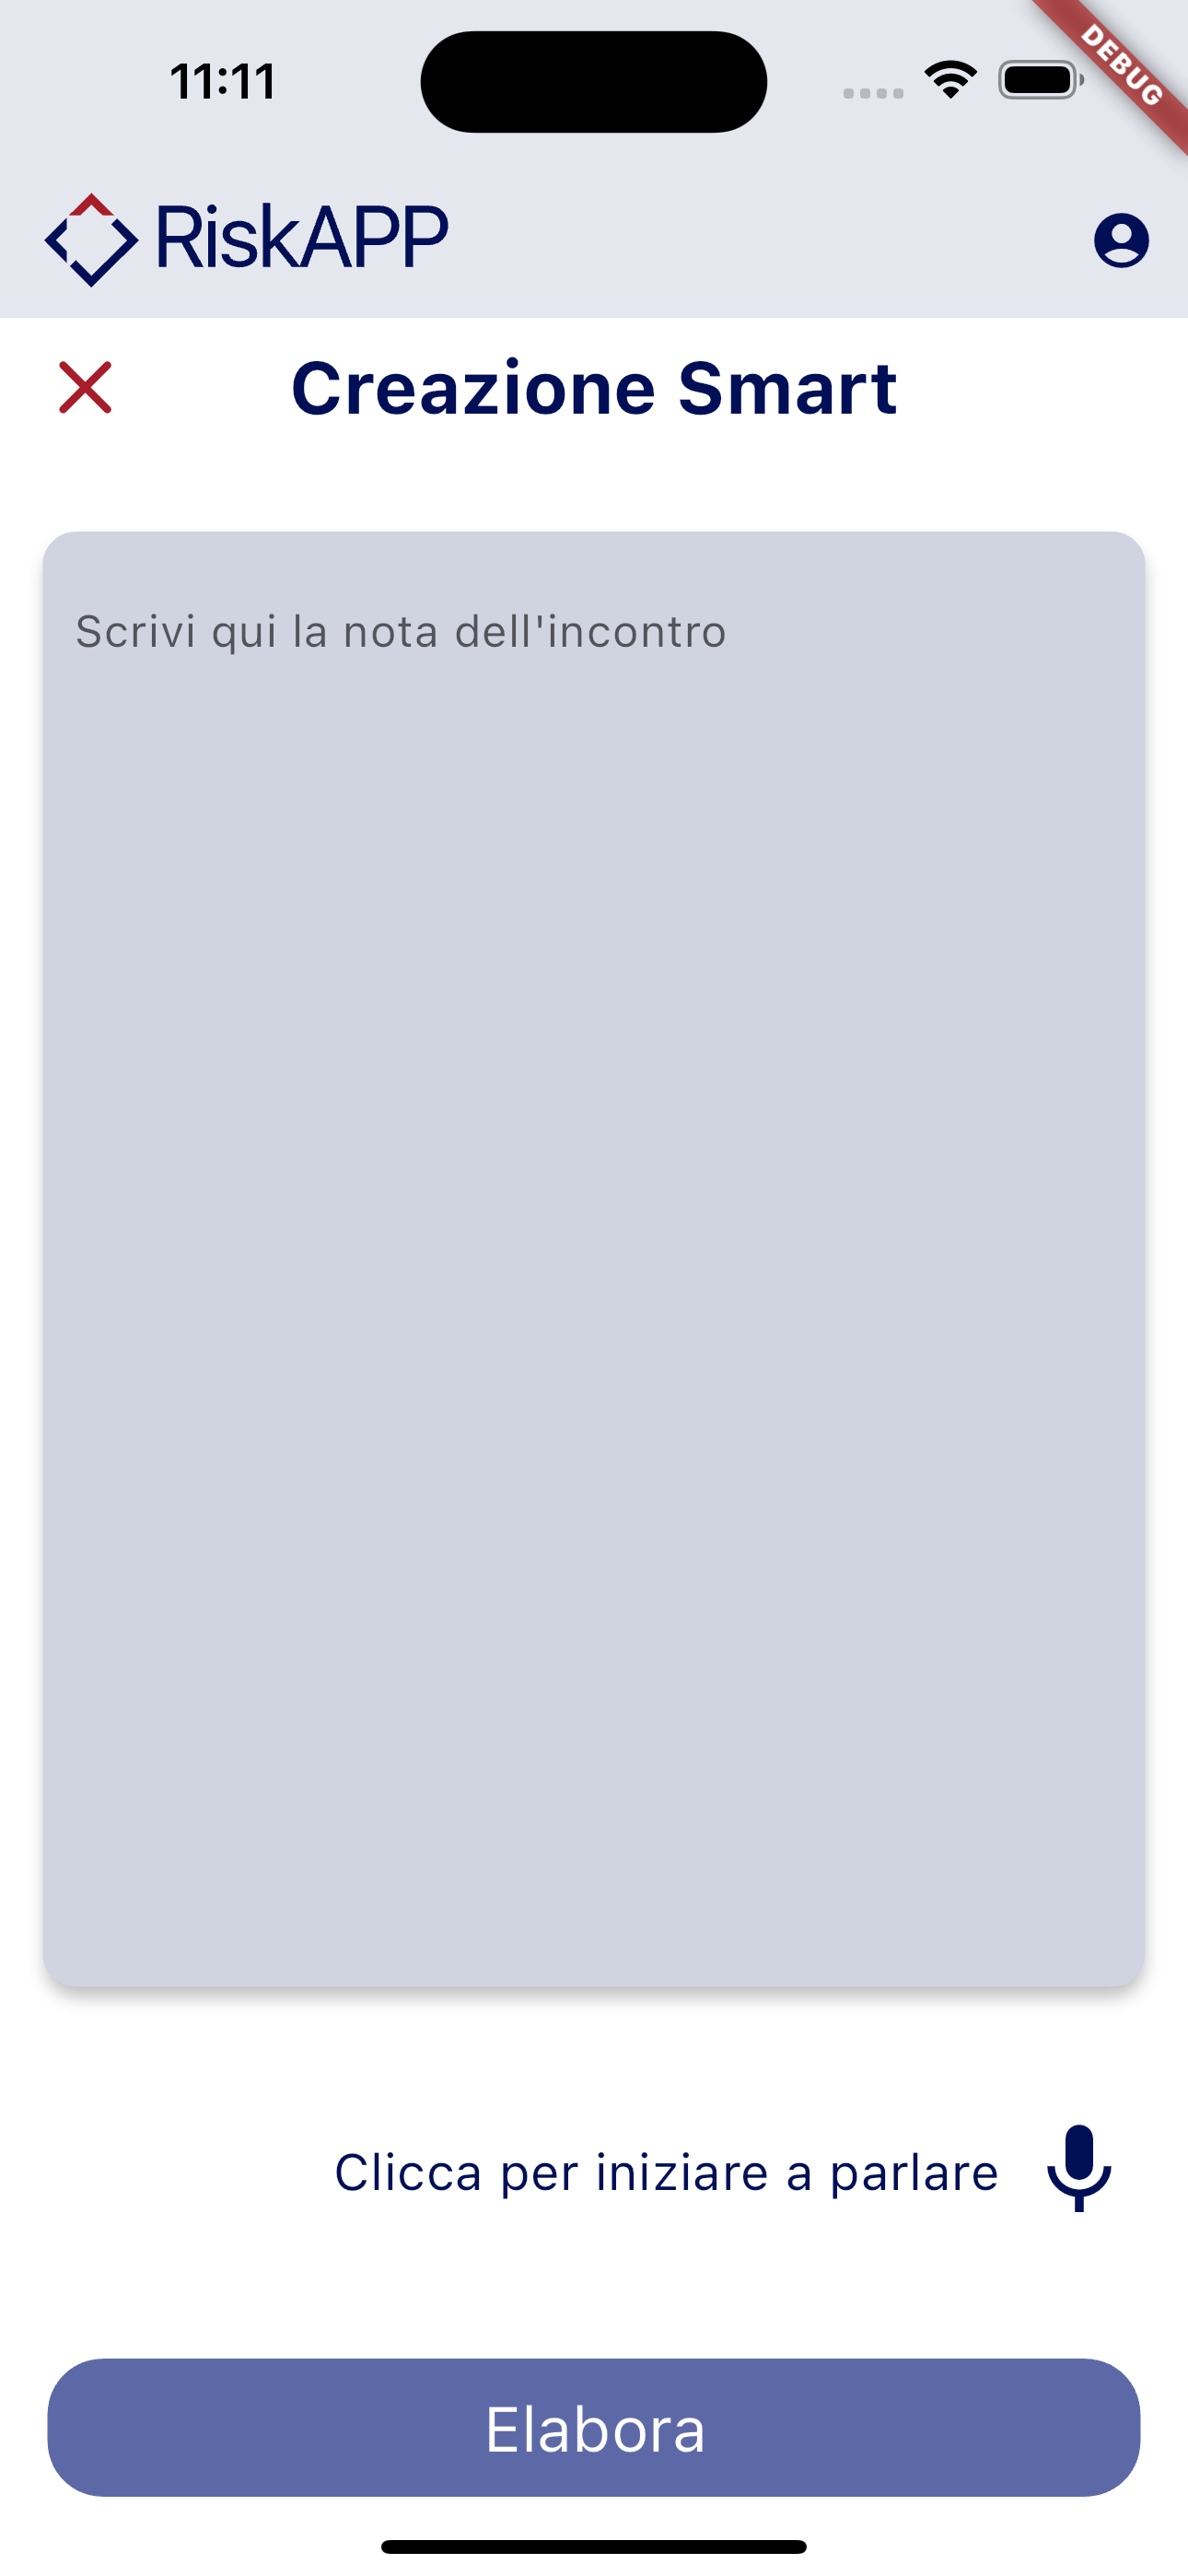
\includegraphics[width=0.3\columnwidth]{screenshot/36-smart_screen} 
    \caption{Smart Creation Screen}
    \label{fig:smart-screen}
\end{figure}

\subsubsection*{ConfirmCreationPopup}
\label{subsubsec:confirm-creation-popup}

Classe che si occupa di mostrare all'utente i dati estratti dall'elaborazione del testo, passati input dal costruttore dall'oggetto di tipo \lstinline{SmartCreationValue} e di permettergli di confermare la creazione della \emph{Meeting Note} o di eventualmente apportare delle modifiche ad alcuni campi. \\
Prima della renderizzazione dell'aspetto grafico viene effettuata l'inizializzazione delle variabili di stato, in particolare:
\begin{itemize}
    \item \lstinline{selectedCategory}, \lstinline{ObjectCategory} che rappresenta la categoria del \gls{cliente}\glsoccur estratto dall'elaborazione del testo;
    \item \lstinline{selectedCategoryIndex}, \lstinline{int} che rappresenta l'indice della categoria del \gls{cliente}\glsoccur;
    \item \lstinline{initialValue}, \lstinline{String} che viene inzializzato con il nome del \gls{cliente}\glsoccur estratto dall'elaborazione del testo;
    \item \lstinline{debouncedSearch} (sezione \ref{subsec:debouncer}), si occupa di gestire la ricerca del \gls{cliente}\glsoccur attraverso il componente \lstinline{CustomAutocomplete};
    \item \lstinline{selectedMeetingNoteObject}, \lstinline{MeetingNoteObject} che si occupa di gestire eventuali modifiche sulla ricerca dell'identificativo del cliente apportate dall'utente ;
    \item \lstinline{isButtonEnabled}, \lstinline{bool} che abilita il pulsante di creazione se tutti i campi sono correttamente compilati;
    \item \lstinline{isNameFound}, \lstinline{bool} che indica se l'identificativo del \gls{cliente}\glsoccur, estratto dall'algoritmo sia stato trovato o meno;
    \item \lstinline{selectedDate}, \lstinline{DateTime} che rappresenta la data estratta dall'elaborazione del testo;
    \item \lstinline{textController}, \lstinline{TextEditingController} che si occupa di gestire il contenuto testuale inserito dall'utente.;
\end{itemize}
La struttura di questa modale è la seguente (figura \ref{fig:smart-popup}):
\begin{itemize}
    \item \lstinline{TitleLabel}, mostra il titolo della \emph{label} per ogni campo elencato di seguito;
    \item \lstinline{CustomObjectPicker}, componente che si occupa di mostrare la lista delle categorie dei \glspl{cliente}\glsoccur e di permettere eventualmente all'utente di apportare modifiche, il cui funzionamento è supportato dalle variabili di stato \lstinline{selectedCategory} e \lstinline{selectedCategoryIndex} (sezione \ref{subsec:object-picker});
    \item \lstinline{CustomAutoComplete}, componente che visualizza l'identificativo del cliente e permette all'utente di apportare modifiche effettuando una ricerca, il suo funzionamento è supportato dalle variabili di stato \lstinline{initialValue}, \lstinline{debouncedSearch} e \lstinline{selectedMeetingNoteObject}, imposta inoltre il valore di \lstinline{isNameFound} in base all'esito della ricerca (sezione \ref{subsec:search-bar});
    \item \lstinline{CustomDatePicker}, componente che visualizza la data estratta dall'elaborazione del testo e permette all'utente di apportare modifiche, il suo funzionamento è supportato dalla variabile di stato \lstinline{selectedDate} (sezione \ref{subsec:date-picker});
    \item \lstinline{CustomTextBox}, componente che visualizza il contenuto dell'incontro estratto dall'elaborazione del testo e permette all'utente di apportare modifiche, il suo funzionamento è supportato dalla variabile di stato \lstinline{textController} (sezione \ref{subsec:text-box});
    \item \lstinline{OutlineButton}\cite{site:outline-button}, componente che si occupa di confermare la creazione della \emph{Meeting Note} richiamando il metodo \lstinline{onConfirmation}.
\end{itemize}
Vi sono presenti inoltre due metodi privati, \lstinline{search} e \lstinline{onConfirmation}. \\
Il primo si occupa di effettuare la ricerca dell'identificativo del \gls{cliente}\glsoccur ricevuto input come parametro, con l'ausilio di \lstinline{meetingNoteObjectProvider} (sezione \ref{subsec:meeting-note-object-provider}) e di controllare l'autorizzazione della richiesta con \lstinline{authProvider}, prima di tutto ciò viene assicurata la presenza di connessione ad internet da \lstinline{networkAwareProvider} (sezione \ref{subsec:network-handler}). \\
Vengono gestiti inoltre i vari esiti della richiesta (i medesimi illustrati nella sezione \ref{subsec:model},  paragrafo \emph{Status Response}) e solamente in caso di successo viene restituito il risultato e aggiornato lo stato di \lstinline{selectedMeetingNoteObject}. \\
Mentre il secondo mostra all'utente una finestra di dialogo attraverso la quale si chiede all'utente di confermare la creazione della \emph{Meeting Note} e in caso affermativo viene effettuata la richiesta al \gls{backend}\glsoccur attraverso \lstinline{meetingNoteProvider} (sezione \ref{subsec:meeting-note-provider}), seguendo poi lo stesso algoritmo descritto sopra.

\subsubsection*{TitleLabel}
\label{subsubsec:title-label}

Classe privata che estende \lstinline{StatelessWidget} e definisce solamente l'aspetto grafico del titolo per la label di ogni campo della \emph{Meeting Note}.

\begin{figure}[!h] 
    \centering 
    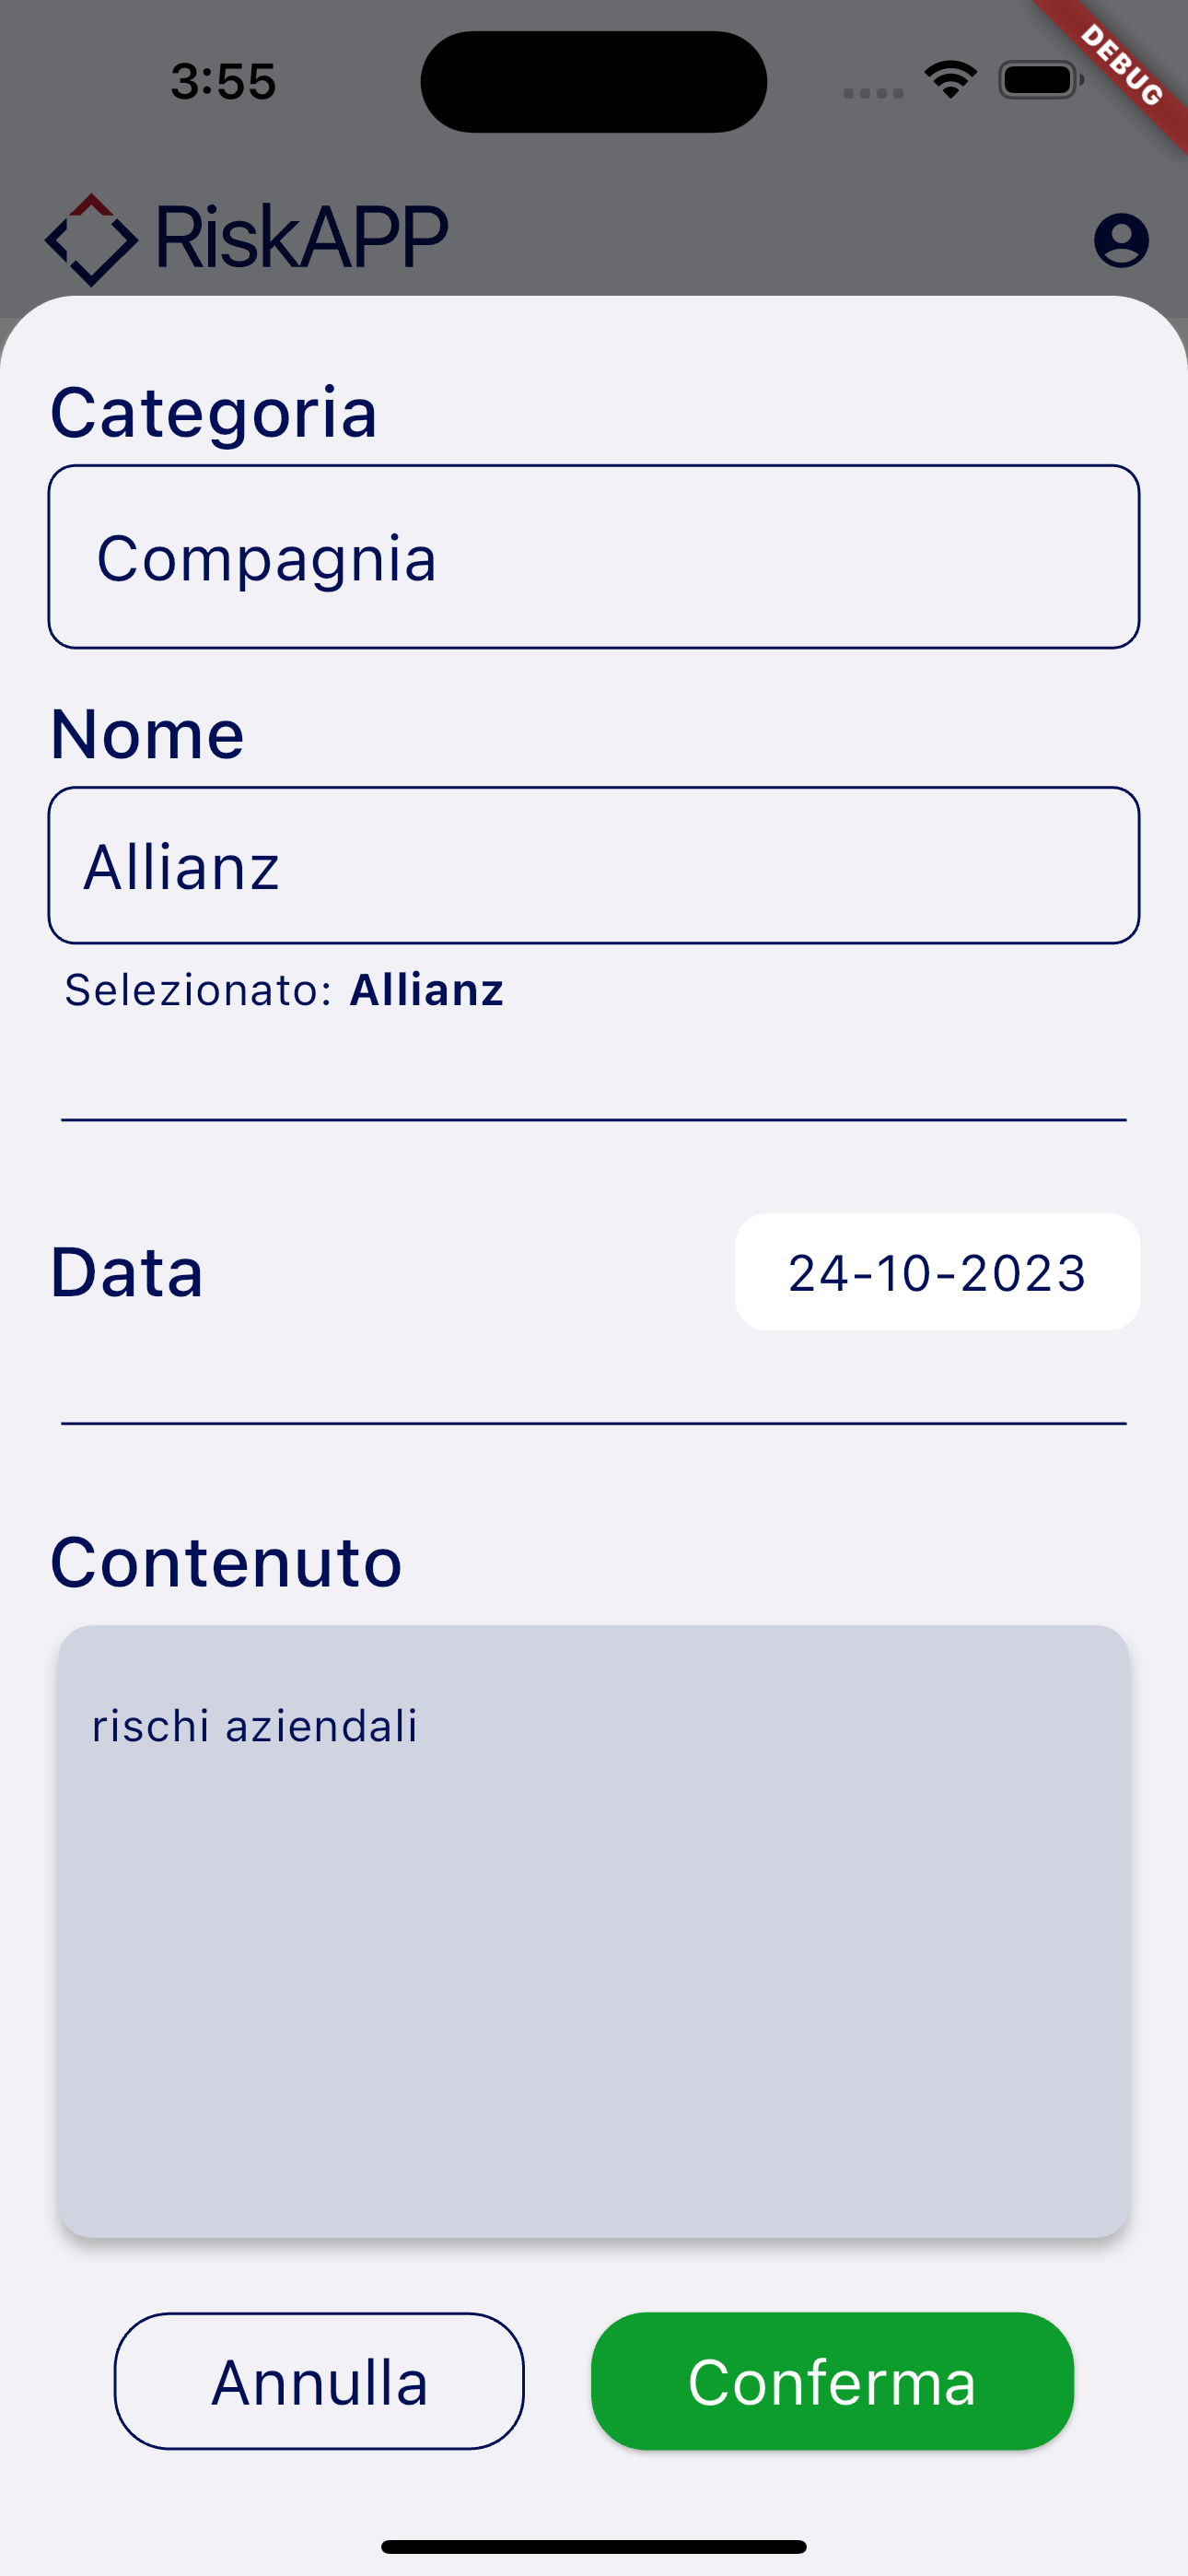
\includegraphics[width=0.3\columnwidth]{screenshot/30-smart_confirm} 
    \caption{Confirm Creation Popup}
    \label{fig:smart-popup}
\end{figure}

\subsection{Wizard Screen 1}
\label{subsec:wizard-screen-1}

% Classi
    % - WizardPage1 (ConsumerStatefulWidget)
        % - Parametri costruttore
            % - title (String)
            % - meetingNote (MeetingNote)
        % - Variabili di stato -> inizializzate via initState
            % - selectedCategory (ObjectCategory)
            % - selectedCategoryIndex (int)
            % - searchController (TextEditingController)
            % - selectedMeetingNoteObject (MeetingNoteObject)
            % - pagingController (PagingController)
            % - searchTerm (String)
            % - isButtonEnabled (bool)
        % - Provider
            % - meetingNoteObjectProvider
            % - authProvider
            % - networkAwareProvider    
        % - Struttura
            % - WizardScreen
            % - WizardHeader
            % - CustomObjectPicker
            % - CustomSearchBar
            % - MeetingNoteObjectList
            % - ForwardButton
        % - Metodi
            % - initState
            % - dispose
            % - fetchPage
            % - isEditingMode
            % - showWizardPage2
    % - MeetingNoteObjectList (StatefulWidget)
        % - Parametri costruttore
            % - onObjectSelected (Function)
            % - pagingController (PagingController)
            % - isEditingMode (bool)
        % - Variabili di stato -> initState
            % - selectedIndex (int)
        % - Struttura
            % - PagedListView
            % - MeetingNoteObjectItem
        % - Metodi
            % - initState
    % - MeetingNoteObjectItem (StatefulWidget)
        % - Parametri costruttore
            % - isContractor (bool)
            % - vatNumber (String)
            % - name (String)
            % - index (int)
            % - selectedIndex (int)
            % - onTap (Function)
        % - Struttura
            % - ListTile
            % - title (Text) -> identificativo cliente
            % - subtitle (Text) -> se isContractor == true


Schermata inerente al primo \emph{step} per la creazione/modifica di una \emph{Meeting Note}, data la sua complessità, essa è stata suddivisa in classi, di cui verranno descritte nel dettaglio. 

\subsubsection*{WizardPage1}
\label{subsubsec:wizard-page-1}

Per comprendere in quale modalità viene richiamato il \gls{wizard}\glsoccur è presente un metodo privato \lstinline{isEditingMode} che restituisce \lstinline{true} se l'utente sta modificando una \emph{Meeting Note} e \lstinline{false} se sta creando una nuova \emph{Meeting Note}. \\
Questo avviene controllando l'oggetto \lstinline{MeetingNote} passato in input alla classe \lstinline{WizardPage1} se è vuoto, in tal caso l'utente sta creando una nuova \emph{Meeting Note}, altrimenti sta modificando una \emph{Meeting Note} esistente. \\
Prima della renderizzazione dell'aspetto grafico viene effettuata l'inizializzazione delle variabili di stato, in particolare:
\begin{itemize}
    \item \lstinline{selectedCategory}, \lstinline{ObjectCategory} che assume il valore della categoria del cliente della \emph{Meeting Note} passata in input se l'utente sta modificando, altrimenti viene inizializzato di \emph{deafult} con \lstinline{ObjectCategory.broker};
    \item \lstinline{selectedCategoryIndex}, \lstinline{int} che assume il valore dell'indice della categoria del cliente della \emph{Meeting Note} passata in input se l'utente sta modificando, altrimenti viene inizializzato di \emph{deafult} con \lstinline{0};
    \item \lstinline{searchController}, \lstinline{TextEditingController} che assume il valore dell'identificativo del cliente della \emph{Meeting Note} passata in input se l'utente sta modificando, altrimenti viene inizializzato di \emph{deafult} con una stringa vuota;
    \item \lstinline{selectedMeetingNoteObject}, \lstinline{MeetingNoteObject} che assume il valore del cliente della \emph{Meeting Note} passata in input se l'utente sta modificando, altrimenti viene inizializzato di \emph{deafult} con \lstinline{null};
    \item \lstinline{pagingController}, \lstinline{PagingController} che si occupa di gestire la paginazione dei dati;
    \item \lstinline{searchTerm}, \lstinline{String} che assume il valore dell'identificativo del cliente della \emph{Meeting Note} passata in input se l'utente sta modificando con il conseguente aggiornamento di \lstinline{pagingController}, altrimenti viene inizializzato di \emph{deafult} con una stringa vuota;
    \item \lstinline{isButtonEnabled}, \lstinline{bool} che abilita il pulsante di creazione se tutti i campi sono correttamente compilati e viene inizializzato a \lstinline{true} se l'utente sta modificando.
\end{itemize}
Per la definizione dell'aspetto grafico questa schermata implementa \lstinline{WizardScreen} (sezione \ref{subsec:screens-template}) e il suo contenuto è strutturato come segue (figura \ref{fig:w1}):
\begin{itemize}
    \item \lstinline{WizardHeader}, imposta il titolo della schermata;
    \item \lstinline{CustomObjectPicker}, componente che si occupa di mostrare la lista delle categorie dei \glspl{cliente}\glsoccur e di permettere all'utente di effettuare una selezione, aggiornando di conseguenza \lstinline{pagingController} e filtrando la lista dei clienti con la categoria selezionata, il suo funzionamento è supportato dalle variabili di stato \lstinline{selectedCategory} e \lstinline{selectedCategoryIndex} (sezione \ref{subsec:object-picker});
    \item \lstinline{CustomSearchBar}, componente che visualizza l'identificativo del cliente e permette all'utente di effettuare una ricerca, aggiornando eventualmente \lstinline{pagingController} e filtrando opportunamente la lista dei clienti, il suo funzionamento è supportato dalle variabili di stato \lstinline{searchController} e \lstinline{searchTerm} (sezione \ref{subsec:search-bar});
    \item \lstinline{MeetingNoteObjectList}, componente che si occupa di mostrare la lista dei clienti opportunamente filtrata e paginata, il suo funzionamento è supportato dalle variabili di stato \lstinline{selectedMeetingNoteObject}, il cui scopo è di evidenziare quale cliente è stato selezionato e \lstinline{pagingController};
    \item \lstinline{ElevatedButton}\cite{site:elevated-button}, componente che si occupa di confermare la selezione del cliente e di mostrare la schermata successiva del \gls{wizard}\glsoccur.
\end{itemize}
Nel dettaglio, prima della visualizzazione della lista paginata, si effettua un controllo dello stato della connessione ad internet attraverso il \lstinline{NetworkAwareProvider} (sezione \ref{subsec:network-handler}), in caso di assenza di connessione viene mostrato un \lstinline{WarningAlert} (sezione \ref{subsec:warning-alert}) con il relativo messaggio di errore. \\
Sono presenti dei metodi privati a supporto del funzionamento del \gls{wizard}\glsoccur, che sono:
\begin{itemize}
    \item \lstinline{fetchPage}, si occupa di effettuare la richiesta al \gls{backend}\glsoccur attraverso il \lstinline{MeetingNoteObjectProvider} (sezione \ref{subsec:meeting-note-object-provider}), controllando se l'utente è autorizzato ad effettuare la richiesta attraverso il metodo \lstinline{isUnauthorized} fornito da \lstinline{authProvider} ( sezione \ref{subsec:authentication-provider}), per poi restituire la lista dei clienti e aggiornare lo stato del \lstinline{PagingController};
    \item \lstinline{isEditingMode}, discusso all'inizio di questa sezione;
    \item \lstinline{showWizardPage2}, si occupa di mostrare la schermata successiva del \gls{wizard}\glsoccur, passando in input l'oggetto \lstinline{MeetingNote}, solamente in caso di modifica, e l'oggetto \lstinline{MeetingNoteObject} selezionato dall'utente.
\end{itemize}

\subsubsection*{MeetingNoteObjectList}
\label{subsubsec:meeting-note-object-list}

\indent Classe che si occupa di mostrare la lista dei clienti opportunamente filtrata e paginata. \\
Attraverso il costruttore riceve in input il \lstinline{PagingController}, la funzione \lstinline{onObjectSelected} che si occupa di aggiornare lo stato di \lstinline{selectedMeetingNoteObject} e la variabile \lstinline{isEditingMode} per evidenziare il cliente selezionato dall'utente. \\

\indent Prima della renderizzazione dell'aspetto grafico viene effettuata l'inizializzazione della variabile di stato \lstinline{selectedIndex} che assume il valore \lstinline{0} (si precisa che il conteggio degli elementi della lista parte da \lstinline{0} e non da \lstinline{1}) se l'utente sta modificando, in quanto la lista in questa modalità mostra solamente un elemento, altrimenti viene inizializzato a \lstinline{-1} per indicare che nessun elemento è stato ancora selezionato. \\
Per la definizione dell'aspetto grafico questa schermata implementa \lstinline{StatefulWidget} e il suo contenuto è strutturato sostanzialmente da \lstinline{PagedListView}\cite{site:infinite-scroll-pagination}, componente che si occupa di mostrare la lista paginata dei clienti, in particolare si avvale del \lstinline{PagingController} per gestire la paginazione dei dati, inoltre per ogni elemento della lista viene mostrato un \lstinline{MeetingNoteObjectItem} (sezione \ref{subsubsec:meeting-note-object-item}) che rappresenta il cliente e permette all'utente di selezionarlo.

\subsubsection*{MeetingNoteObjectItem}
\label{subsubsec:meeting-note-object-item}

Classe che si occupa di visualizzare il cliente in un \emph{item} della lista e permette all'utente di selezionarlo. \\
Attraverso il costruttore riceve in input i seguenti parametri:
\begin{itemize}
    \item \lstinline{isContractor}, \lstinline{bool} che indica se il cliente è un \gls{cliente}\glsoccur appartiene alla categoria dei \emph{contraenti};
    \item \lstinline{vatNumber}, \lstinline{String} che rappresenta la partita iva del contraente;
    \item \lstinline{name}, \lstinline{String} che rappresenta l'identificativo del cliente;
    \item \lstinline{index}, \lstinline{int} che rappresenta l'indice del cliente nella lista;
    \item \lstinline{selectedIndex}, \lstinline{int} che rappresenta l'indice del cliente selezionato dall'utente;
    \item \lstinline{onTap}, \lstinline{Function} che si occupa di impostare \lstinline{selectedIndex} con l'indice del cliente selezionato dall'utente.
\end{itemize}
Per la definizione dell'aspetto grafico questa schermata implementa \lstinline{StatefulWidget} e il suo contenuto è strutturato sostanzialmente da \lstinline{ListTile}\cite{site:list-tile}, \emph{widget} che si occupa di mostrare il cliente nella lista, in particolare si avvale dei parametri \lstinline{title} e \lstinline{subtitle} per mostrare rispettivamente l'identificativo del cliente e la sua partita iva, inoltre evidenzia l'\emph{item} del cliente selezionato variandone il colore di sfondo e del testo.\\
Per capire quale cliente è stato selezionato dall'utente viene effettuato una comparazione del valore di \lstinline{selectedIndex} e \lstinline{index}.

\begin{figure}[!h] 
    \centering 
    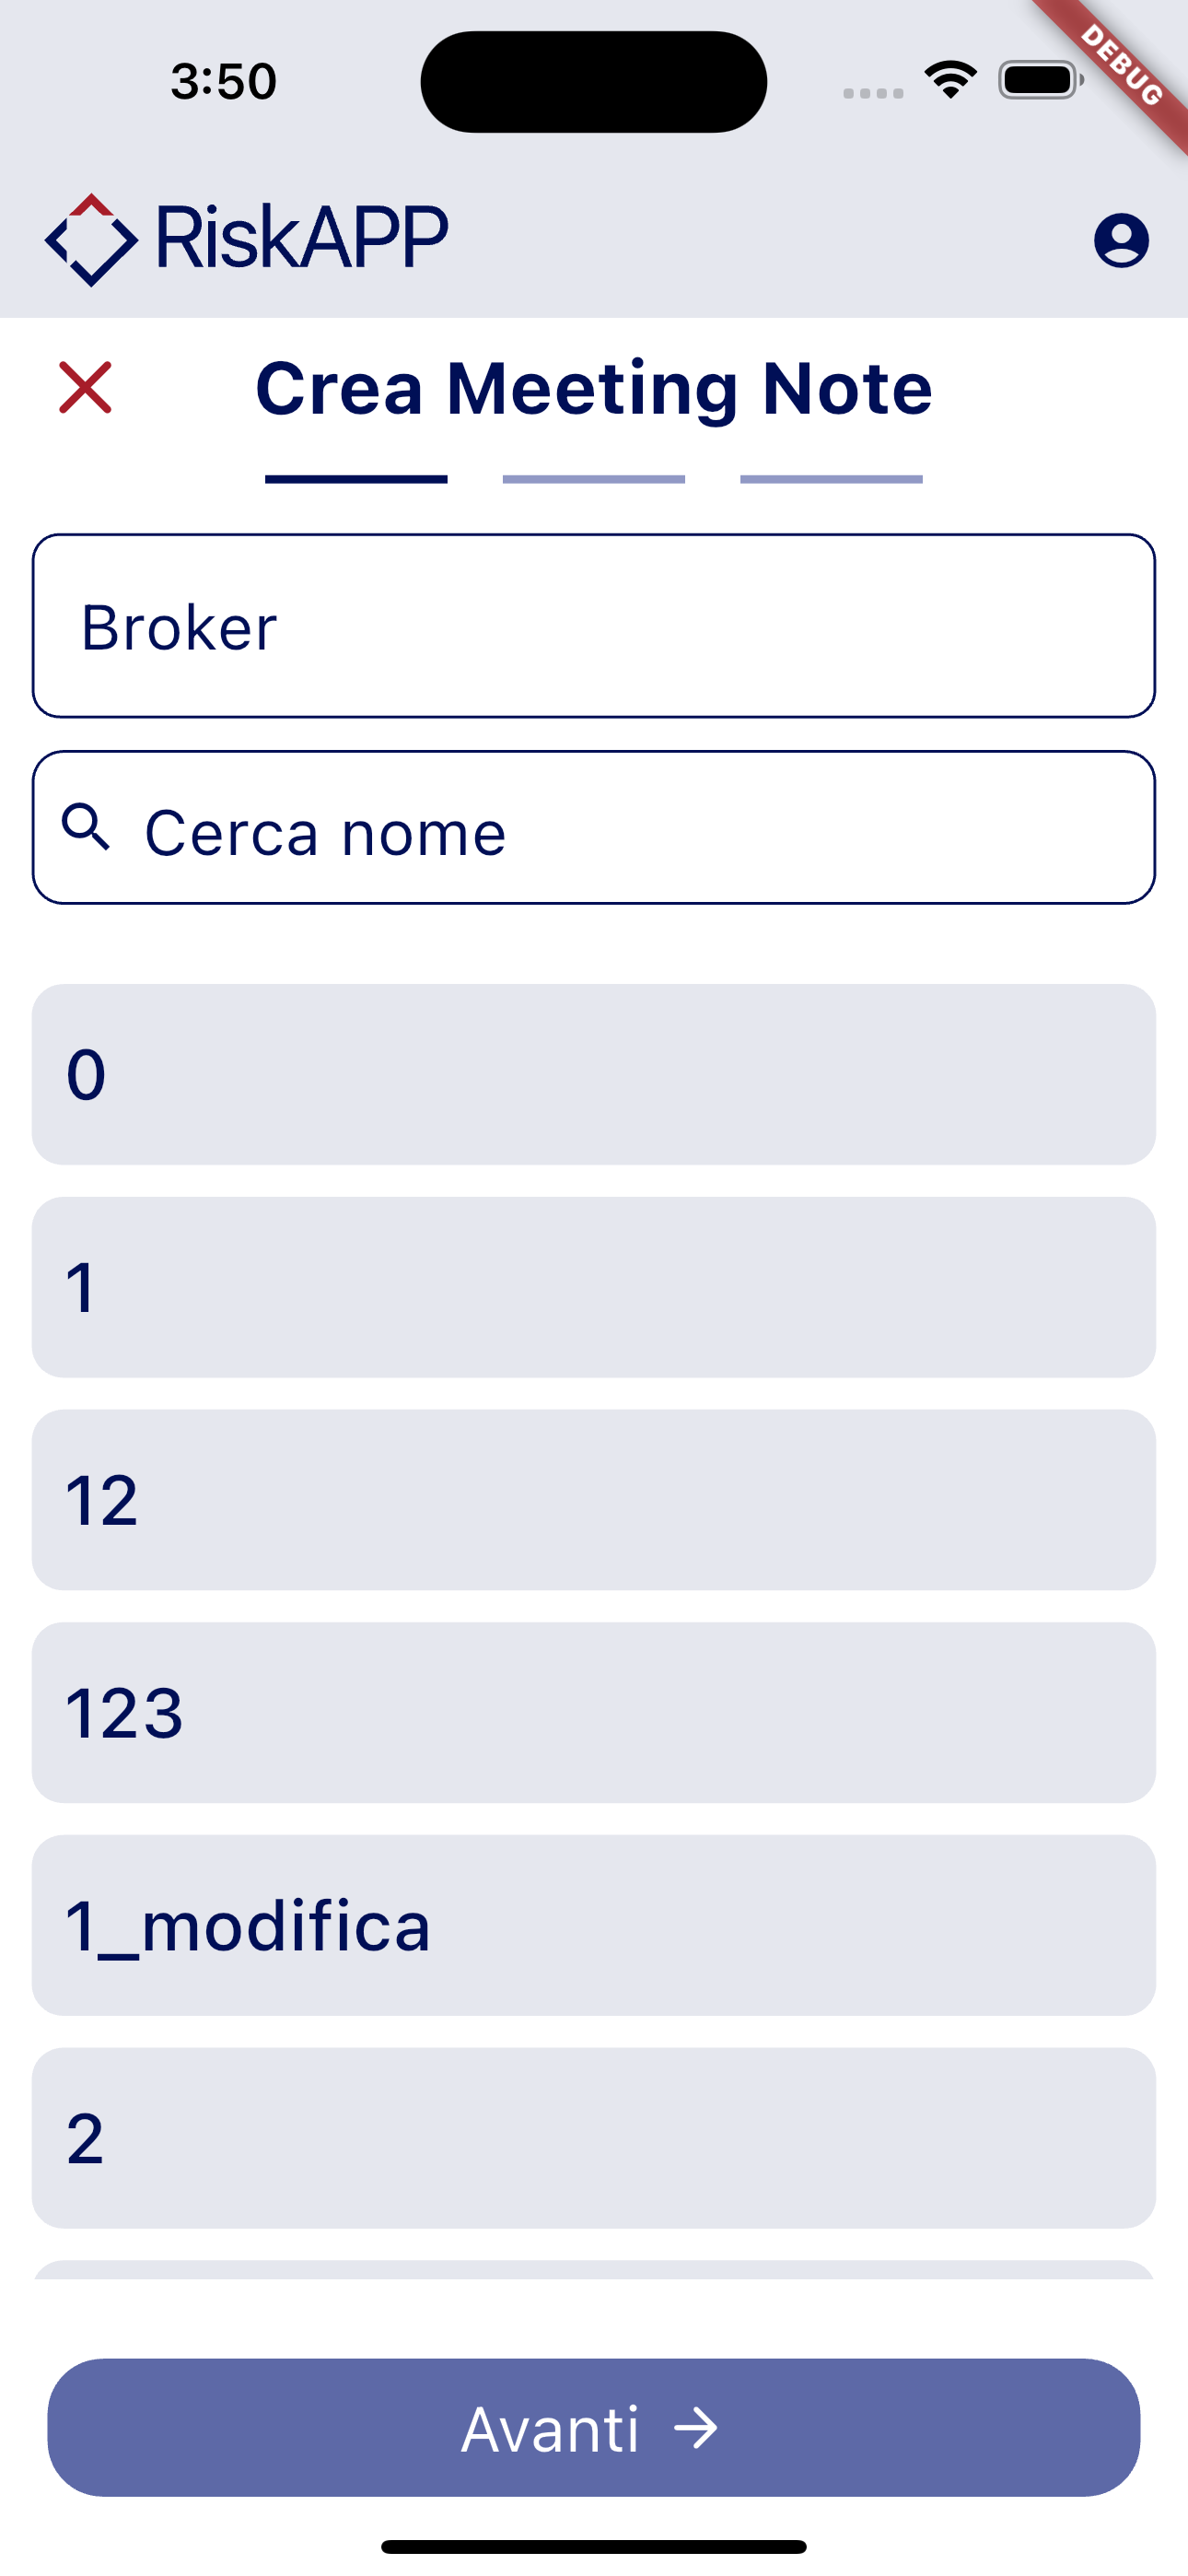
\includegraphics[width=0.3\columnwidth]{screenshot/15-wc1}
    \hfill
    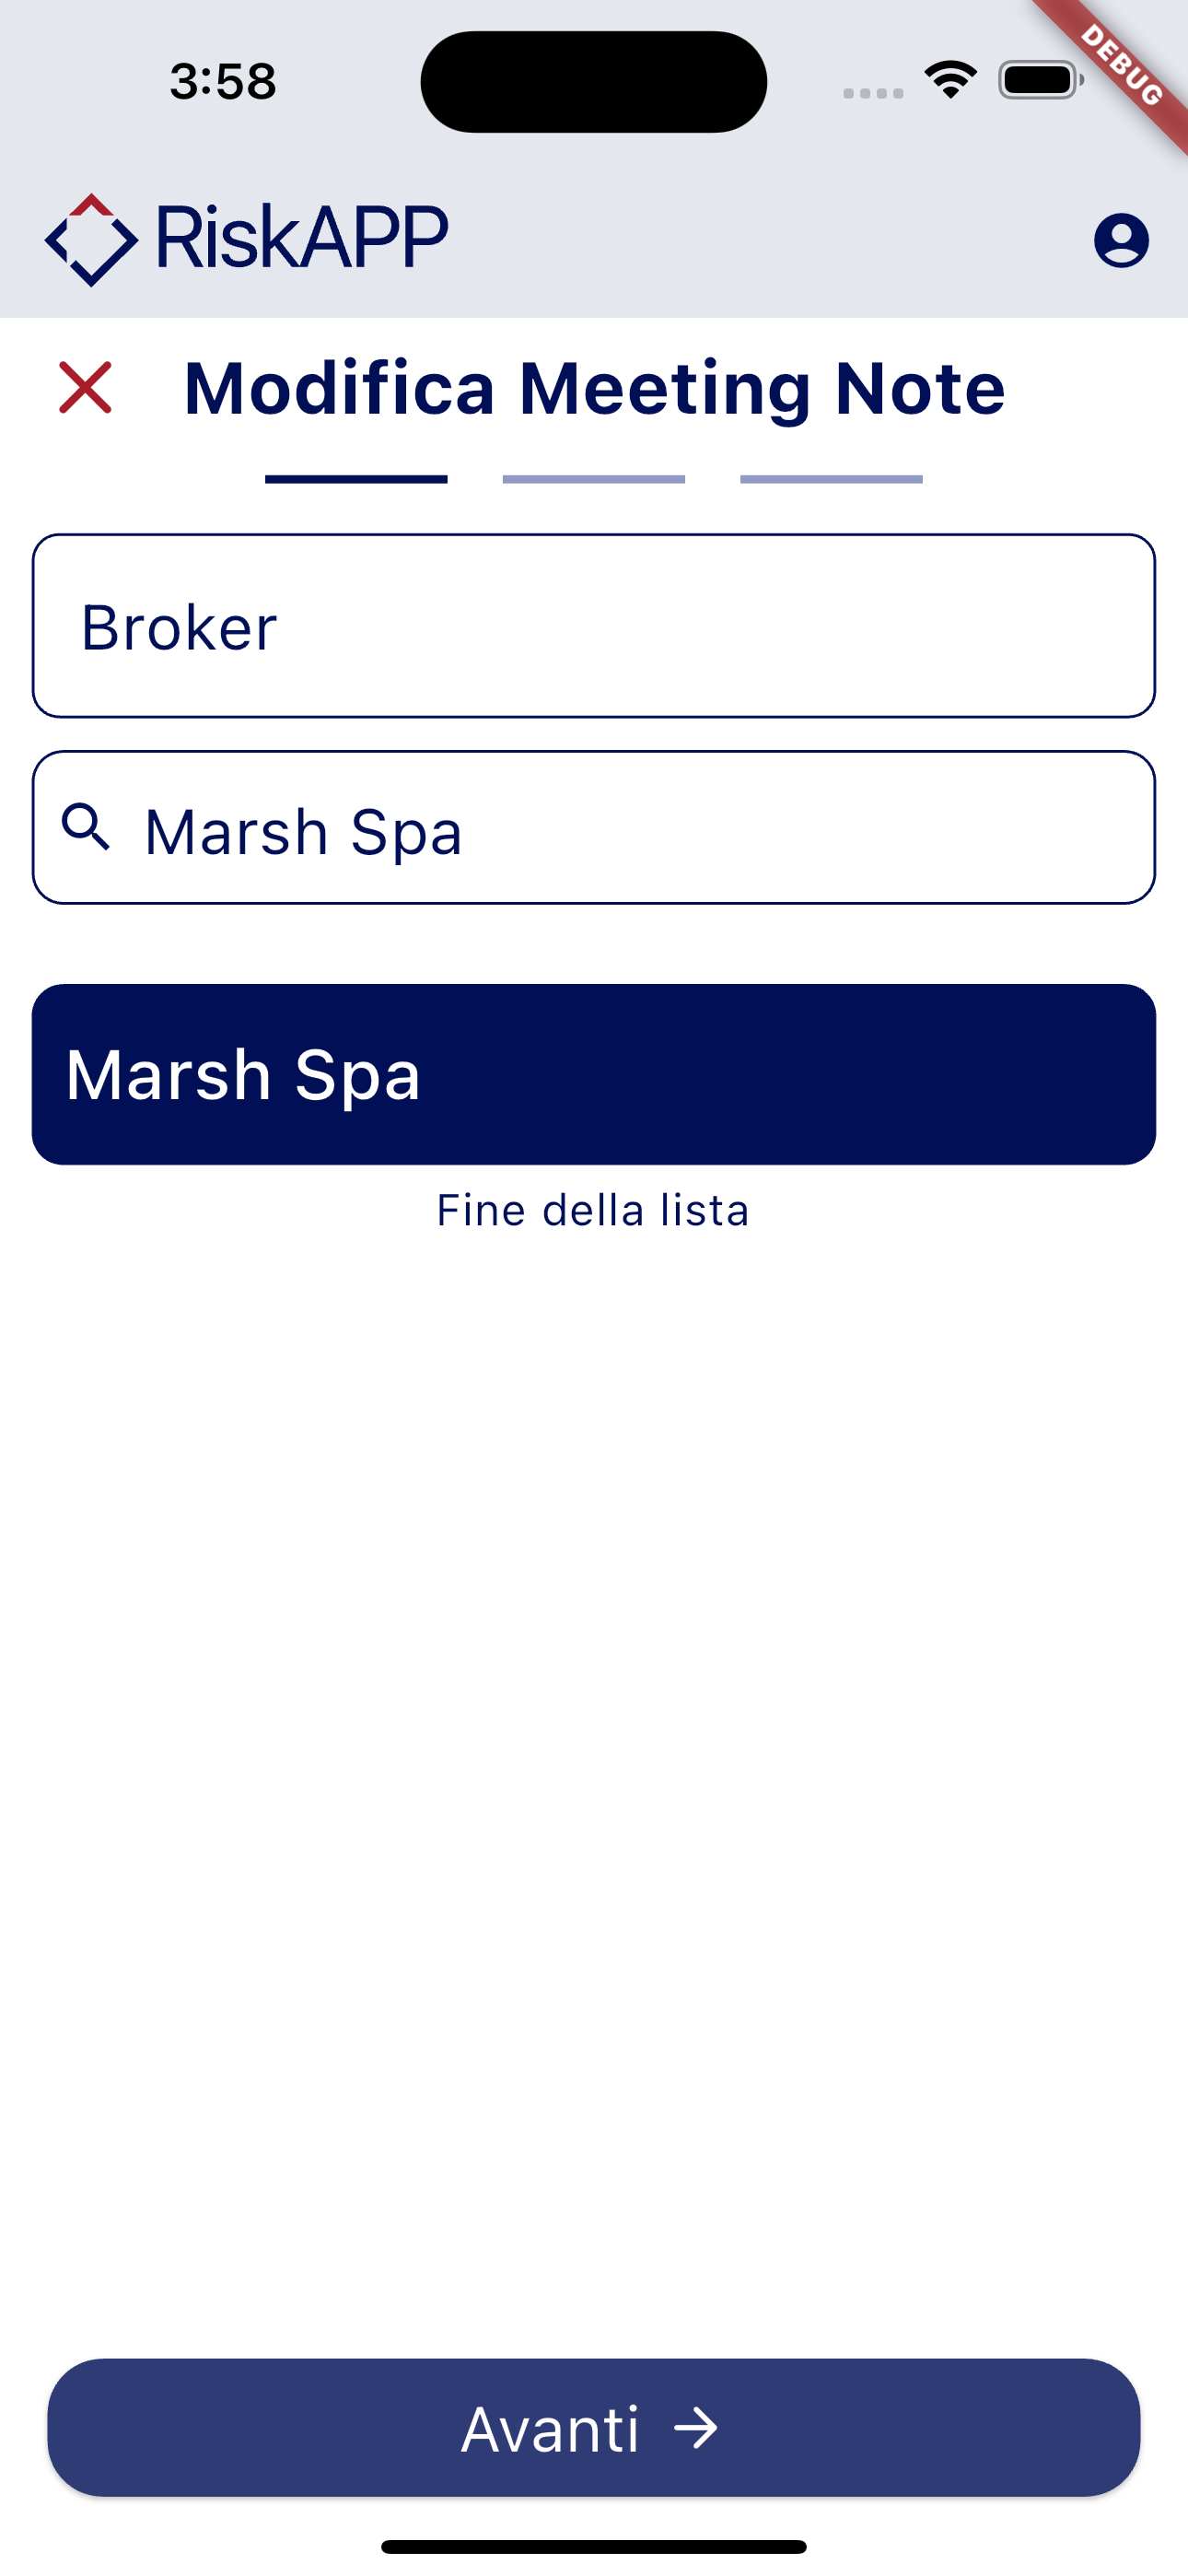
\includegraphics[width=0.3\columnwidth]{screenshot/32-wm1} 
    \caption{Wizard Screen 1 - Creazione e Modifica}
    \label{fig:w1}
\end{figure}

\subsection{Wizard Screen 2}
\label{subsec:wizard-screen-2}

% Classi 
    % - WizardPage2 (StatefulWidget)
        % - Parametri costruttore
            % - title (String)
            % - meetingNoteObject (MeetingNoteObject)
            % - meetingNote (MeetingNote)
        % - Variabili di stato -> inizializzate via initState
            % - selectedDate (DateTime)
        % - Provider -> NESSUNO
        % - Struttura
            % - WizardScreen
            % - WizardHeader
            % - CustomScrollDatePicker
            % - ForwardButton
            % - BackButton
        % - Metodi 
            % - initState
            % - showWizardPage3

Schermata inerente al secondo \emph{step} per la creazione/modifica di una \emph{Meeting Note}. \\
Prima della renderizzazione dell'aspetto grafico viene effettuata l'inizializzazione della variabile di stato \lstinline{selectedDate} che assume il valore della data della \emph{Meeting Note} passata in input se l'utente sta modificando, altrimenti viene inizializzato di \emph{deafult} con la data corrente (figura \ref{fig:w2}). \\
Per la definizione dell'aspetto grafico questa schermata implementa \lstinline{WizardScreen} (sezione \ref{subsec:screens-template}) e il suo contenuto è strutturato come segue:
\begin{itemize}
    \item \lstinline{WizardHeader}, imposta il titolo della schermata (sezione \ref{subsec:screens-template});
    \item \lstinline{CustomScrollDatePicker}, componente che si occupa di mostrare la data e permette all'utente di selezionarla, il suo funzionamento è supportato dalla variabile di stato \lstinline{selectedDate} (sezione \ref{subsec:scroll-date-picker});
    \item \lstinline{ElevatedButton}\cite{site:elevated-button}, pulsante che si occupa di confermare la selezione della data e di renderizzare alla schermata successiva del \gls{wizard}\glsoccur invocando il metodo \lstinline{showWizardPage3};
    \item \lstinline{OutlinedButton}\cite{site:outline-button}, pulsante che si occupa di renderizzare alla schermata precedente del \gls{wizard}\glsoccur.
\end{itemize}
In questa schermata non è presente alcun \lstinline{Provider} in quanto non è necessario effettuare alcuna richiesta al \gls{backend}\glsoccur, poichè si tratta solamente di effettuare una selezione della data.

\begin{figure}[!h] 
    \centering 
    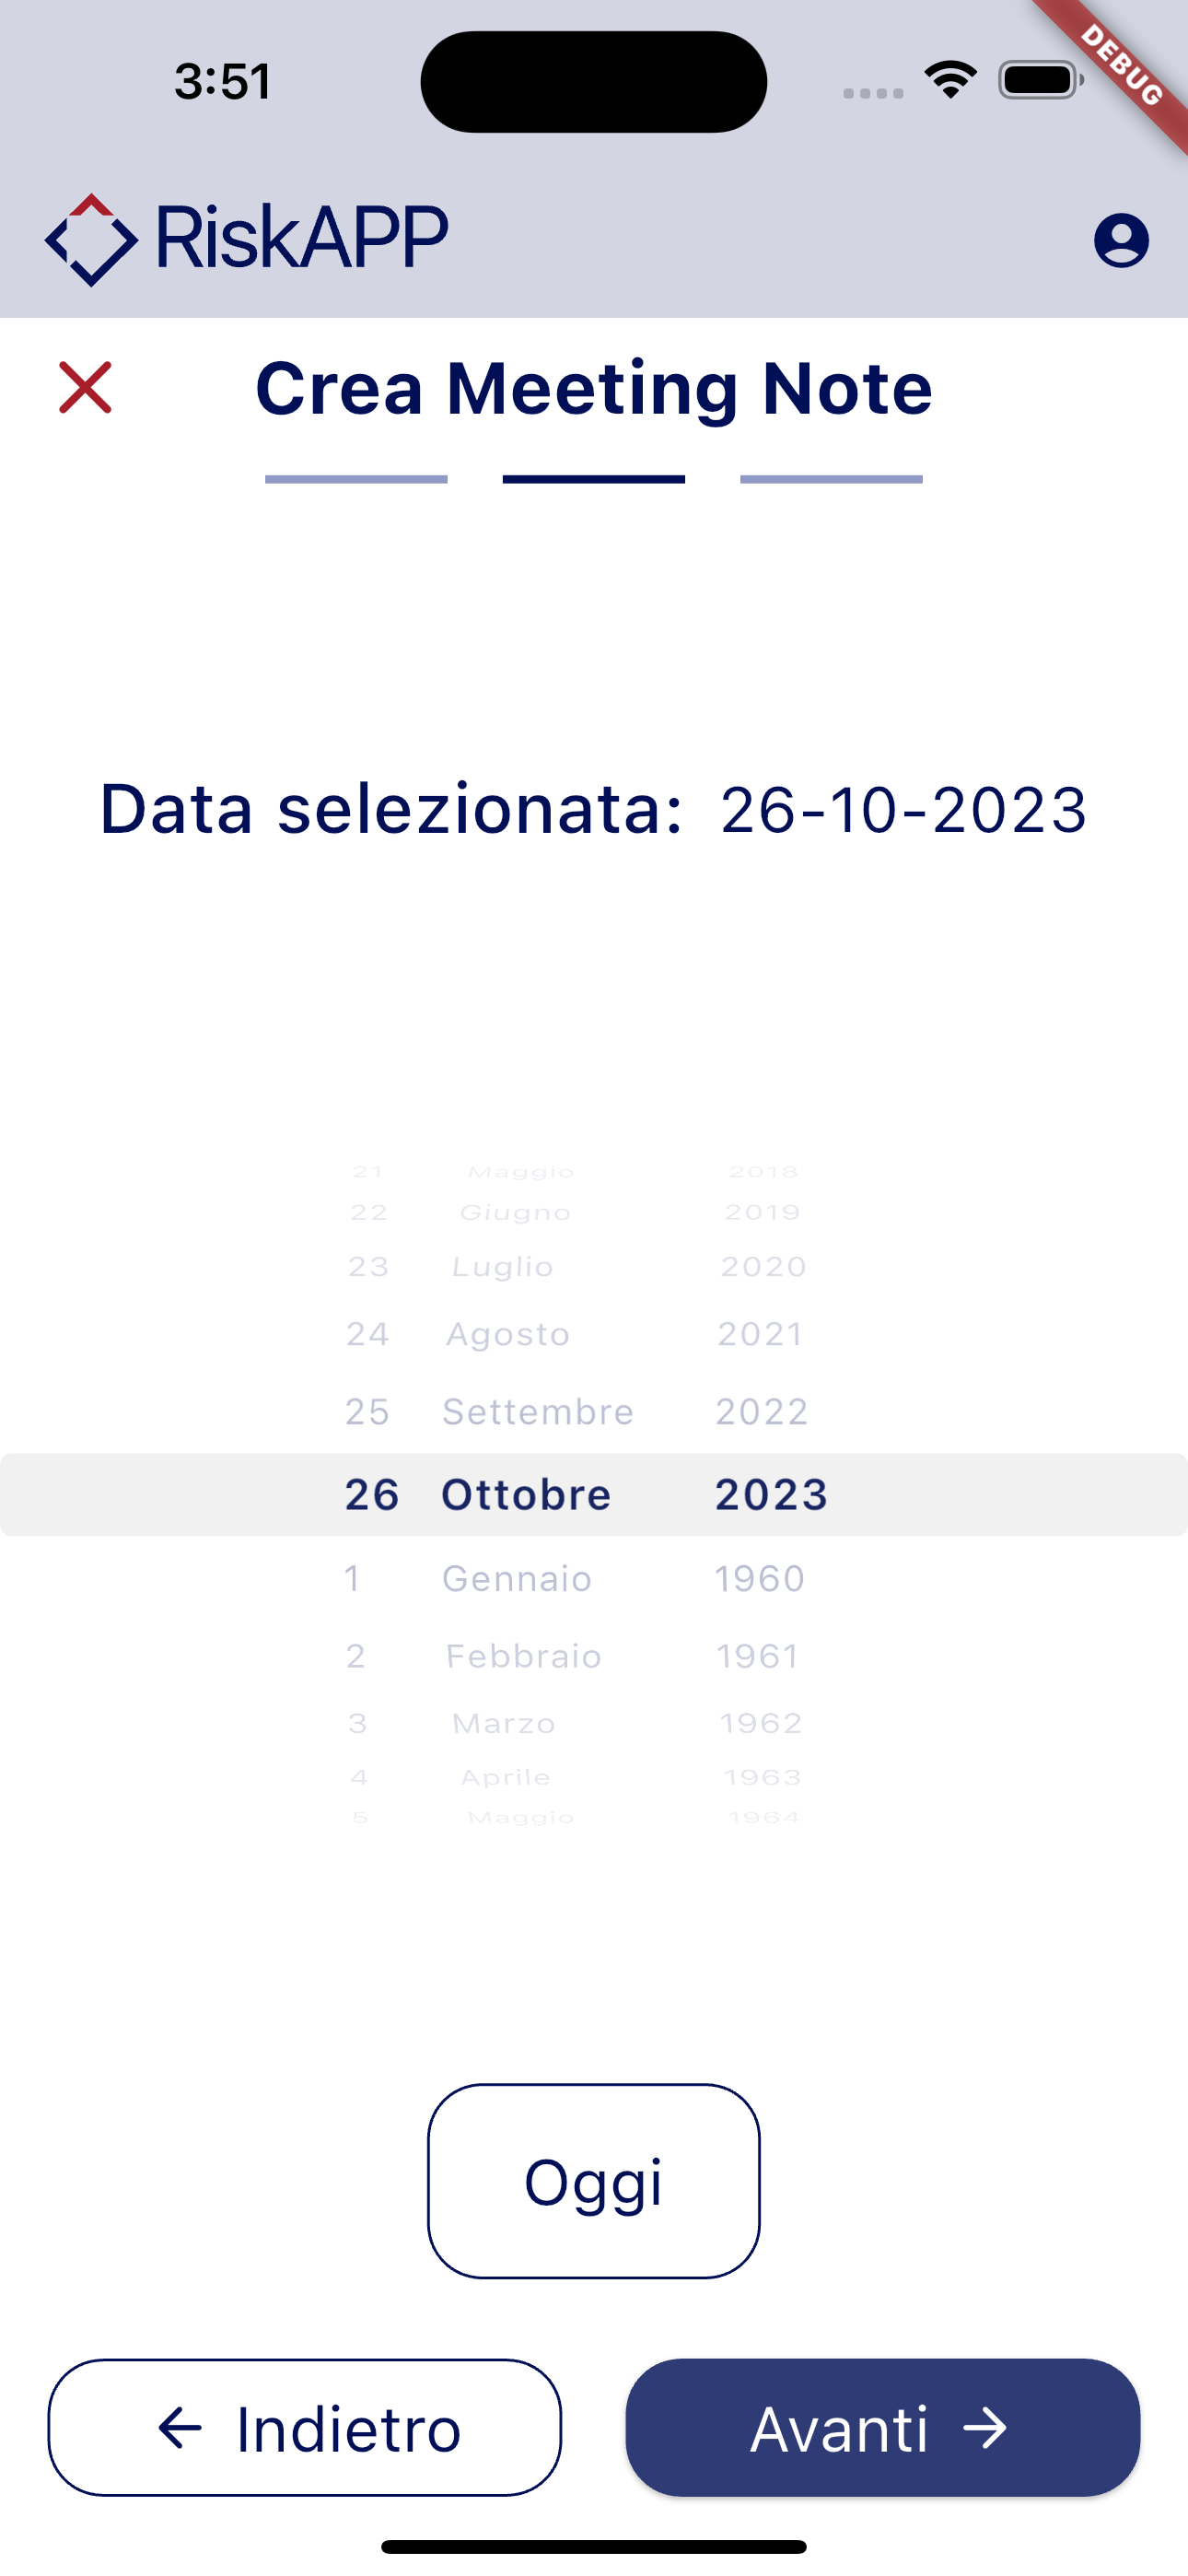
\includegraphics[width=0.3\columnwidth]{screenshot/19-wc2}
    \hfill
    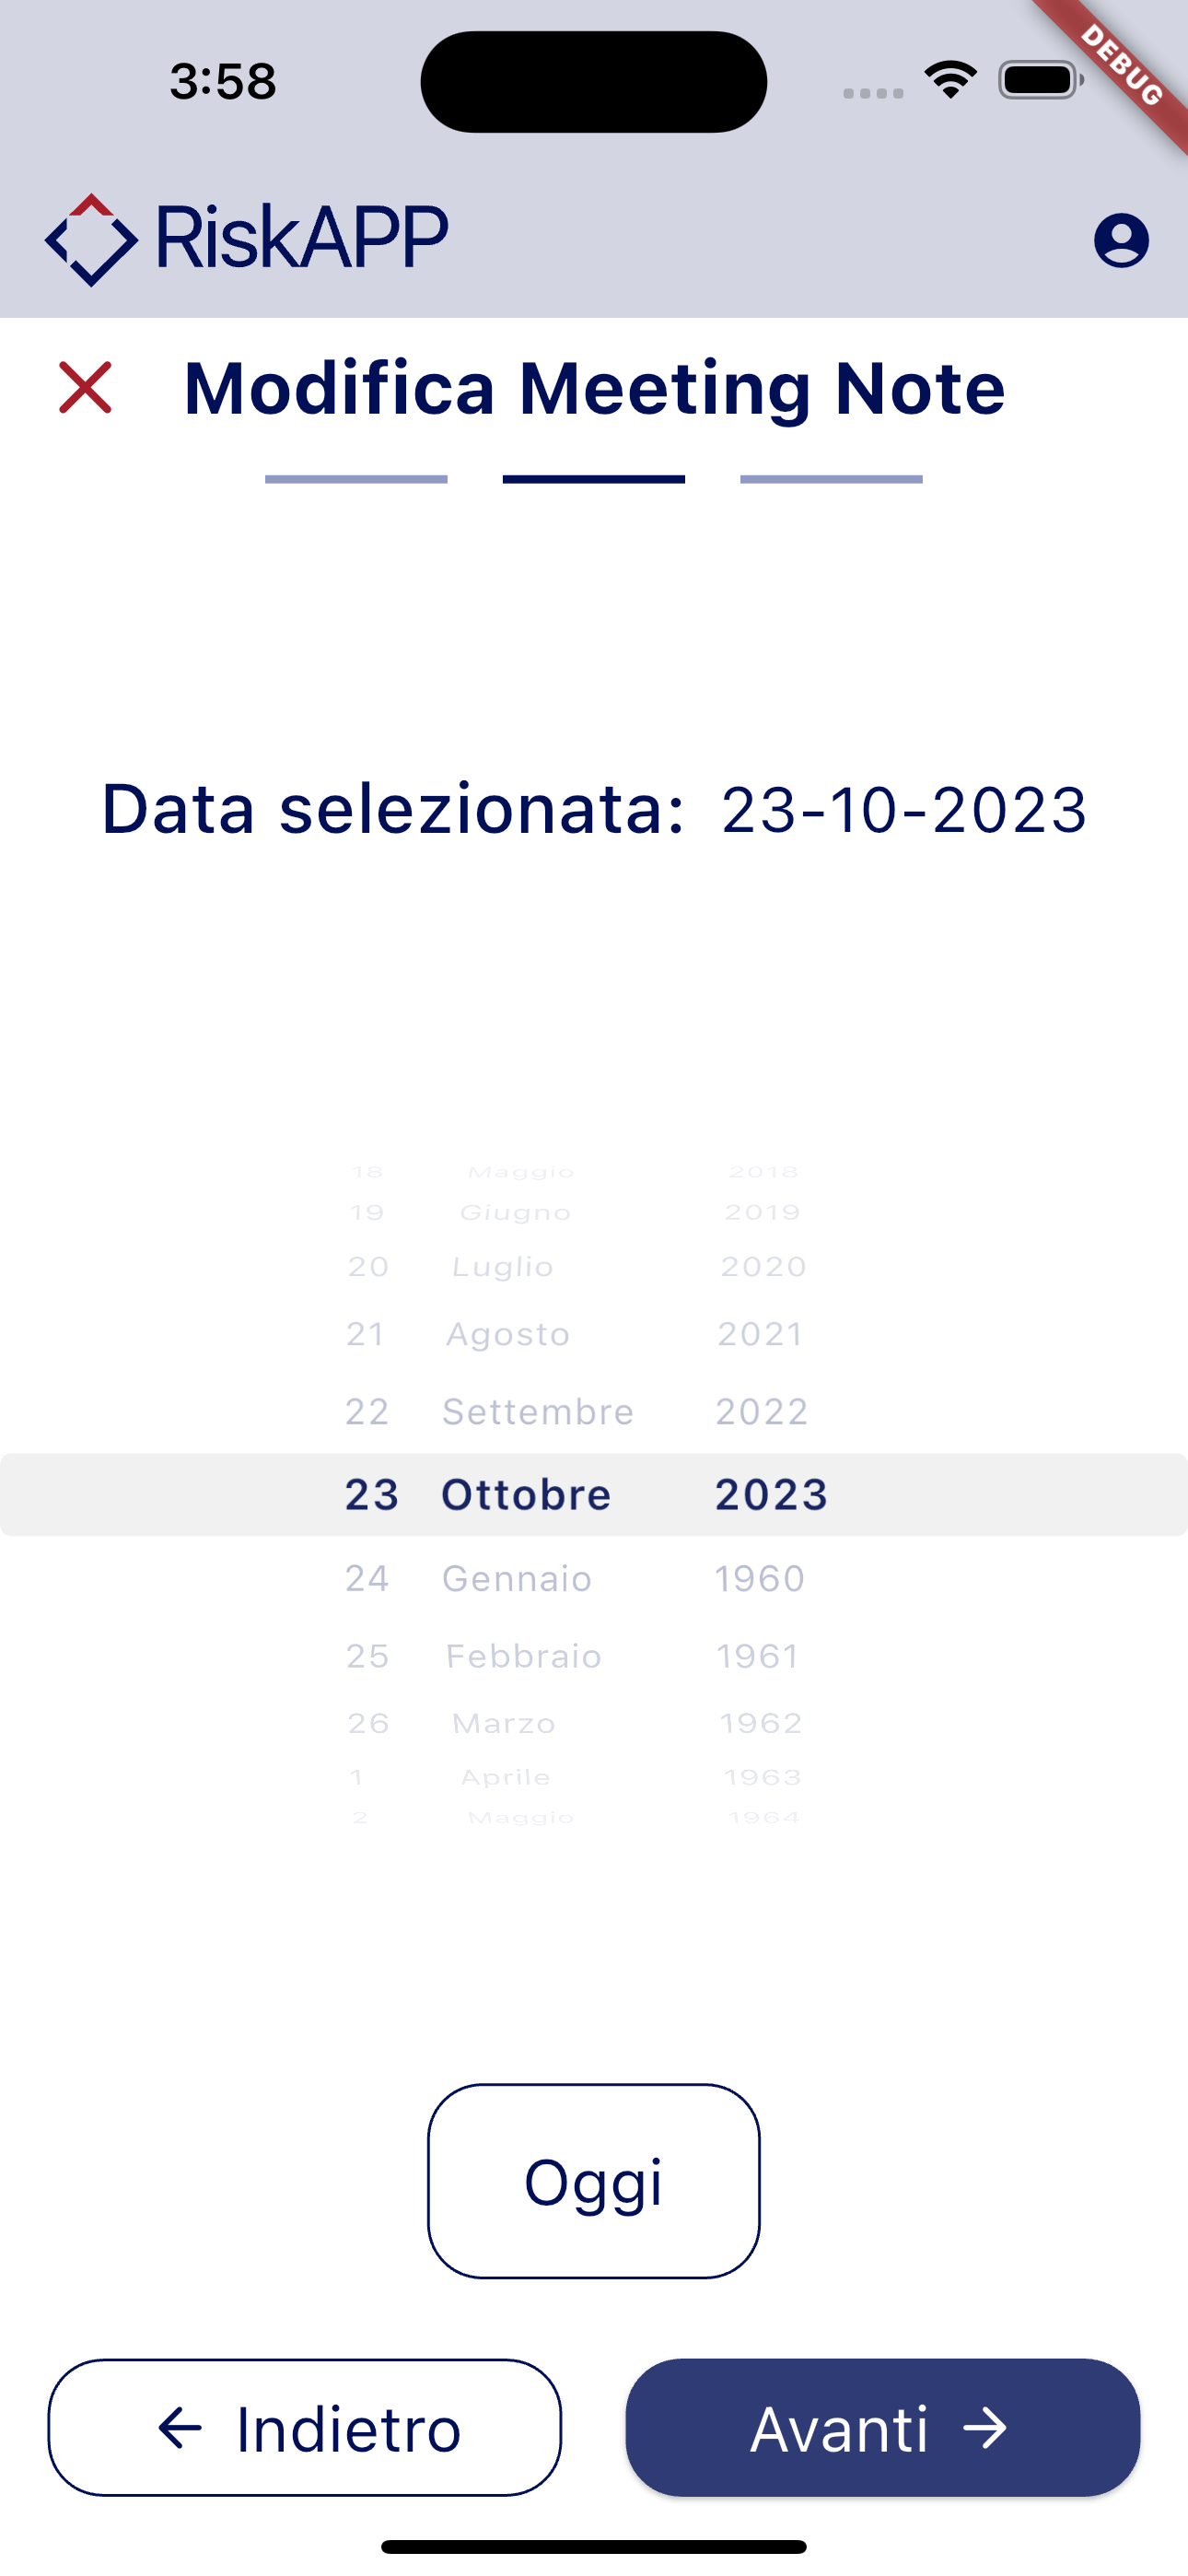
\includegraphics[width=0.3\columnwidth]{screenshot/33-wm2} 
    \caption{Wizard Screen 2 - Creazione e Modifica}
    \label{fig:w2}
\end{figure}


\subsection{Wizard Screen 3}
\label{subsec:wizard-screen-3}

% Classi
    % - WizardPage3 (ConsumerStatefulWidget)
        % - Parametri costruttore
            % - title (String)
            % - meetingNoteObject (MeetingNoteObject)
            % - meetingNoteDate (DateTime)
            % - meetingNote (MeetingNote)
        % - Variabili di stato -> inizializzate via initState
            % - textController (TextEditingController)
            % - isButtonEnabled (bool)
            % - speechToText (SpeechToText)
            % - listenedWords (String)
        % - Provider
            % - meetingNoteProvider
            % - networkAwareProvider
            % - authProvider
        % - Struttura
            % - WizardScreen
            % - WizardHeader
            % - SummaryCard
            % - CustomTextBox
            % - RecordingButton
            % - ConfirmButton
        % - Metodi
            % - initState
            % - dispose
            % - onConfirmation
    % - SummaryCard (privato) (StatelessWidget)     
        % - Parametri costruttore
            % - meetingNoteObject (MeetingNoteObject)
            % - meetingNoteDate (DateTime)
        % - Struttura
            % - Card
            % - Text -> identificativo cliente
            % - Text -> data  

Schermata inerente al terzo \emph{step} per la creazione/modifica di una \emph{Meeting Note}. \\
\lstinline{WizardPage3} è la classe principale che si occupa di ricevere in input il contenuto testuale dall'utente e di permettergli di confermare la creazione della \emph{Meeting Note}. \\
Prima della renderizzazione dell'aspetto grafico viene effettuata l'inizializzazione delle variabili di stato, in particolare:
\begin{itemize}
    \item \lstinline{textController}, \lstinline{TextEditingController} che si occupa di gestire il contenuto testuale inserito dall'utente, se l'utente sta modificando la \emph{Meeting Note}, viene inizializzato con il suo contenuto, altrimenti con una stringa vuota;
    \item \lstinline{isButtonEnabled}, \lstinline{bool} che indica se l'utente ha inserito del testo e abilita di conseguenza il pulsante per confermare la creazione della \emph{Meeting Note};
    \item \lstinline{speechToText}, \lstinline{SpeechToText} che si occupa di gestire la dettatura vocale;
    \item \lstinline{listenedWords}, \lstinline{String} che memorizza quanto detto dall'utente.
\end{itemize}
Per la definizione dell'aspetto grafico questa schermata implementa \lstinline{WizardScreen} (sezione \ref{subsec:screens-template}) e il suo contenuto è strutturato come segue:
\begin{itemize}
    \item \lstinline{WizardHeader}, imposta il titolo della schermata (sezione \ref{subsec:screens-template});
    \item \lstinline{SummaryCard}, classe privata, sviluppata con lo scopo di visualizzare un riepilogo dei dati inseriti dall'utente, il suo funzionamento è supportato dalle variabili di stato \lstinline{meetingNoteObject} e \lstinline{meetingNoteDate}, verrà discussa la sua struttura nel dettaglio in seguito;
    \item \lstinline{CustomTextBox}, componente che si occupa di ricevere in input il contenuto testuale inserito dall'utente, che può avvenire in due modalità differenti come specificato nei requisiti \hyperref[RFN-72]{RFN-72} e \hyperref[RFN-73]{RFN-73} (sezione \ref{subsec:text-box});
    \item \lstinline{RecordingButton}, componente che si occupa attivare la dettatura vocale (sezione \ref{subsec:recording-button});
    \item \lstinline{OutlinedButton}\cite{site:outline-button}, pulsante che si occupa di renderizzare alla schermata precedente del \gls{wizard}\glsoccur;
    \item \lstinline{ElevatedButton}\cite{site:elevated-button}, pulsante che si occupa di confermare la creazione/modifica della \emph{Meeting Note} richiamando il metodo \lstinline{onConfirmation}.
\end{itemize}
Il metodo privato \lstinline{onConfirmation} si occupa di mostrare all'utente una finestra di dialogo attraverso la quale si chiede all'utente di confermare la creazione della \emph{Meeting Note} e in caso affermativo viene effettuata la richiesta al \gls{backend}\glsoccur attraverso \lstinline{meetingNoteProvider} (sezione \ref{subsec:meeting-note-provider}), controllandone l'autorizzazione con \lstinline{authProvider} e gestendo i vari esiti della richiesta (i medesimi illustrati nella sezione \ref{subsec:model},  paragrafo \emph{Status Response}). \\
Per differenziare il caso di creazione a quello di modifica si utilizza lo stesso approccio descritto nella sezione \ref{subsubsec:wizard-page-1}, ovvero si verifica se l'oggetto \lstinline{MeetingNote} passato in input è vuoto, in tal caso l'utente sta creando una nuova \emph{Meeting Note}, altrimenti sta modificando una \emph{Meeting Note} esistente, di conseguenza viene invocato la chiamata opportuna. \\
Prima della gestione degli esiti possibili della richiesta viene effettuato un controllo sullo stato della connessione ad internet attraverso il \lstinline{NetworkAwareProvider} (sezione \ref{subsec:network-handler}), in caso di assenza di connessione viene mostrato un \lstinline{WarningAlert} (sezione \ref{subsec:warning-alert}) con il relativo messaggio di errore. \\
Infine durante l'elaborazione della richiesta viene mostrato una finestra di dialogo mostrando all'utente che l'operazione è in corso.

\begin{figure}[!h] 
    \centering 
    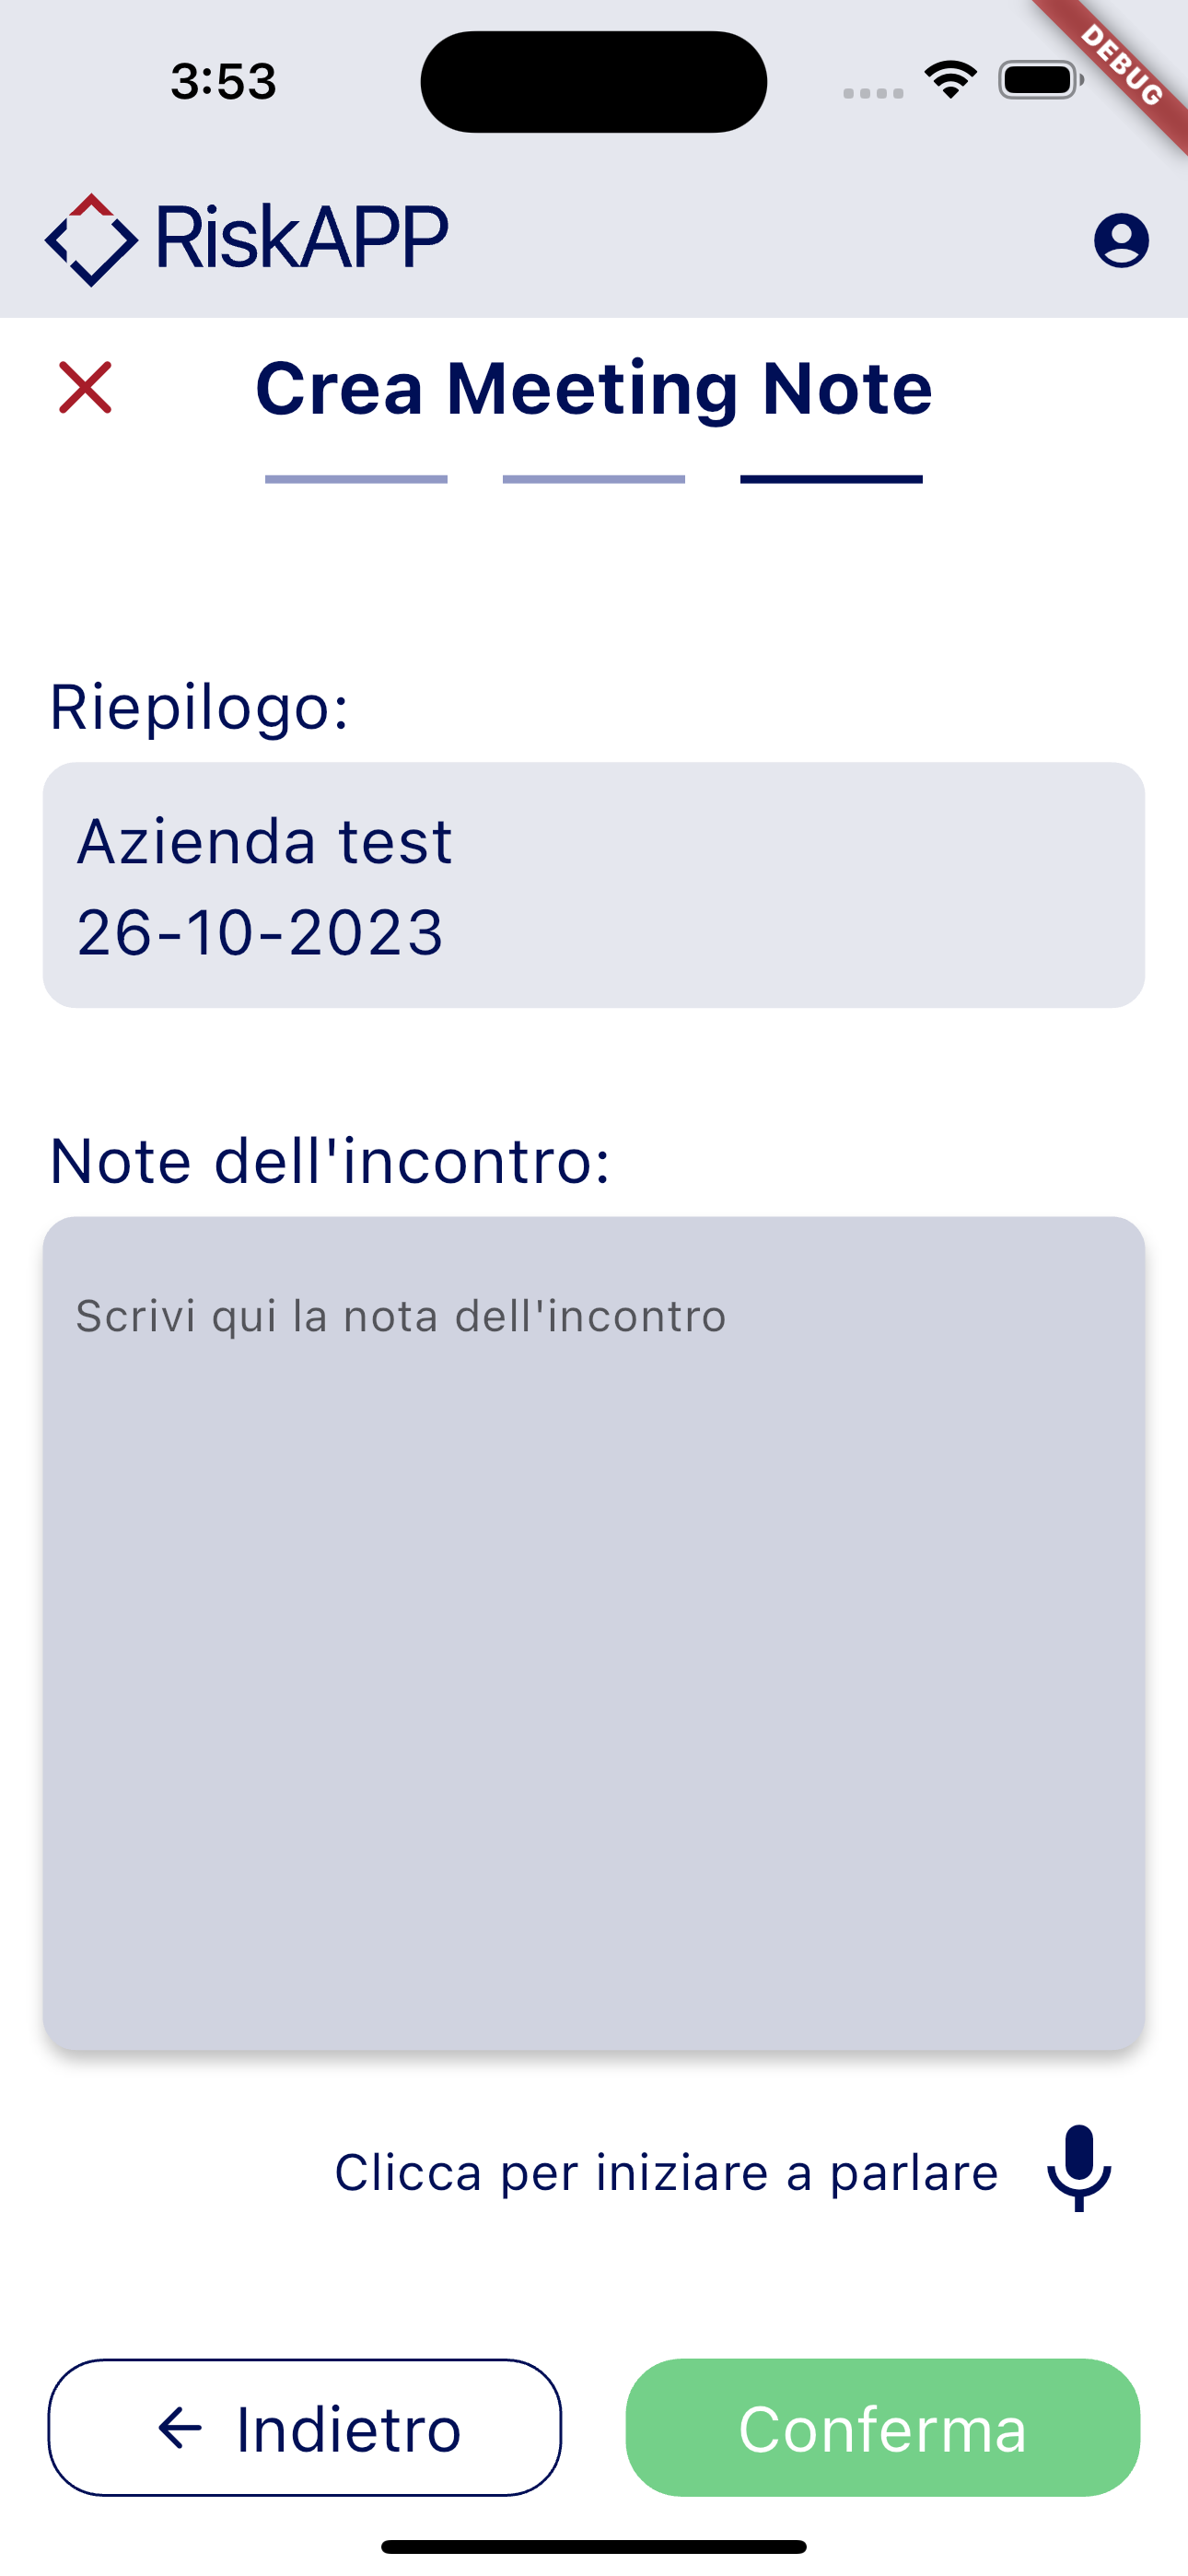
\includegraphics[width=0.3\columnwidth]{screenshot/20-wc3}
    \hfill
    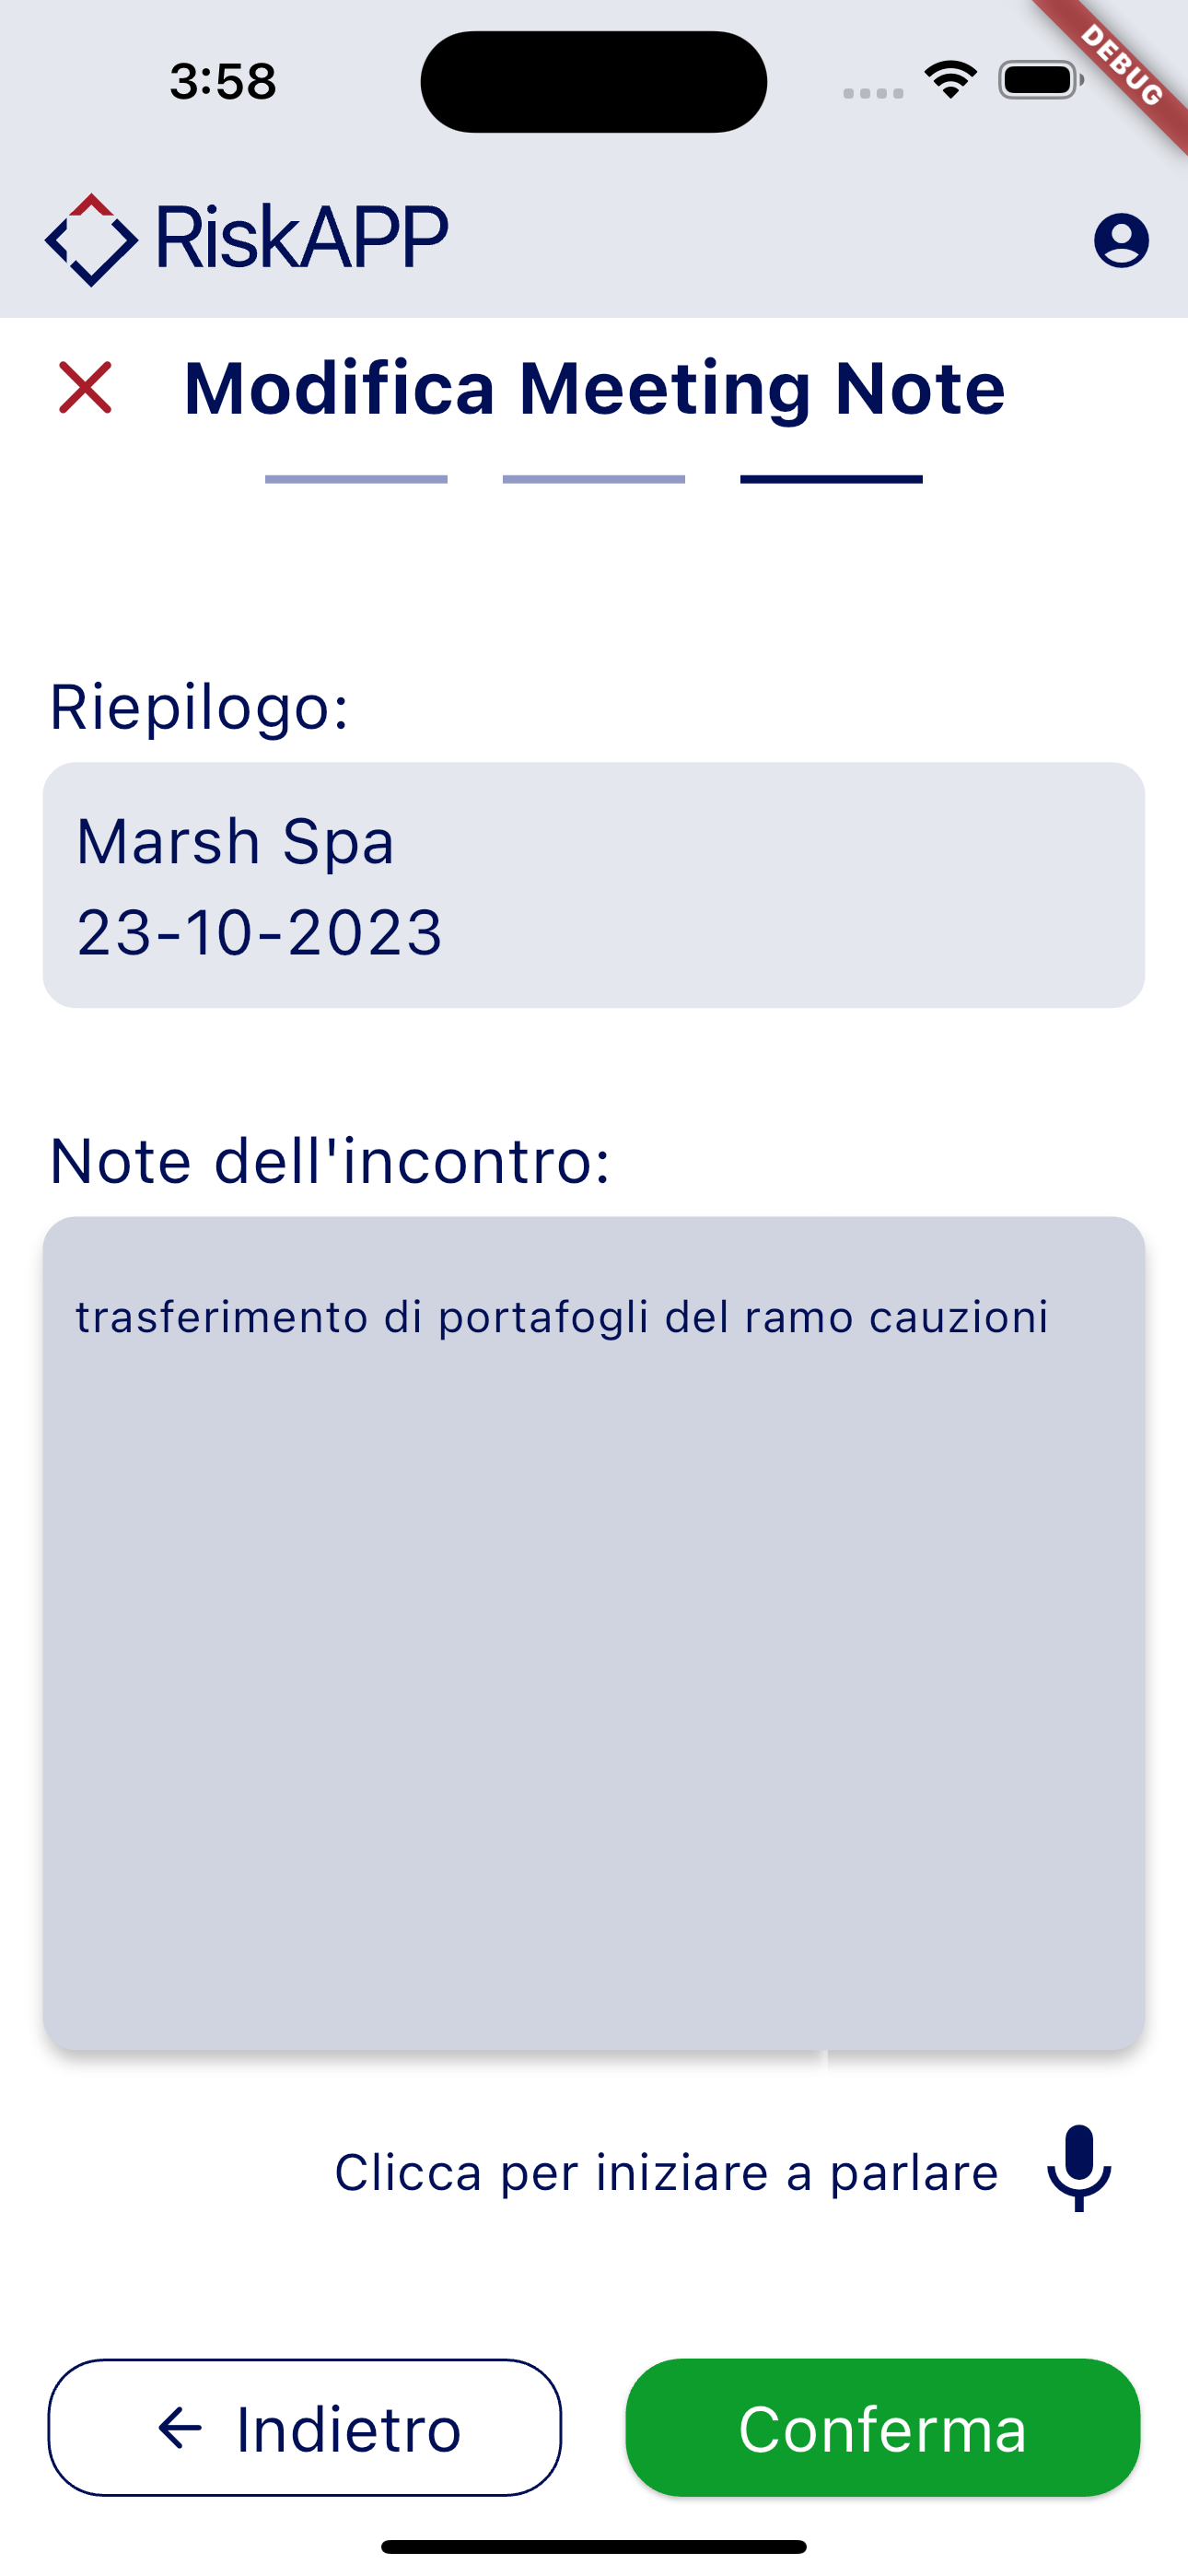
\includegraphics[width=0.3\columnwidth]{screenshot/34-wm3} 
    \caption{Wizard Screen 1 - Creazione e Modifica}
    \label{fig:w3}
\end{figure}

\newpage

\section{Styles}
\label{sec:styles}

% SPIEGARE COME FUNZIONANO I TEMI, OVVERO CHE UNA VOLTA DEFINITO ADEGUATAMENTE E RICHIAMATO NEL MAIN.DART, AI WIDGET IMPLEMENTATI VIENE, generalmente, APPLICATO in maniera AUTOMATICA, altre volte, se si vuole una ulteriore personalizzazione, si usa Theme.of(context).<nome_elemento>.<colore>\\

\emph{Flutter}\cite{site:flutter} per applicare uno stile grafico all'interfaccia si serve della classe \lstinline{Theme}\cite{site:theme-class} in cui viene richiamata nel \lstinline{main.dart} (sezione \ref{sec:main}), la conseguenza è che i \emph{widget} implementati erediteranno lo stile grafico definito. \\
Senza una ridefinizione del tema, verrà applicato quello di \emph{default}, per questo progetto invece, seguendo il \gls{mockup}\glsoccur è stato personalizzato. \\
In particolare è sufficiente ridefinire opportunamente la classe \lstinline{ThemeData}\cite{site:theme-data-class}, che contiene tutta la configurazione grafica dell'applicazione. \\
Per la ridefinizione del tema si sono create delle classi, raccolte in opportuni file, che si occupano di definire i colori, dimensioni e stili grafici utilizzati nell'applicazione. \\
Si specifica che le variabili utilizzate per la configurazione sono definite come \lstinline{static const}, in quanto devono essere accessibili senza la necessità di istanziare la classe. \\
Di seguito verrà illustrato nel dettaglio il contenuto di ogni file.

\subsection{AppColors}
\label{subsec:app-colors}

\lstinline{AppColors} è una classe in cui viene ridefinita la \emph{palette} colori utilizzata nell'applicazione, in particolare:
\begin{itemize}
    \item \lstinline{primary}, rappresenta il colore primario, applicato ai compomenti principali dell'applicazione (es. pulsanti, icone, ecc.);
    \item \lstinline{secondary}, rappresenta il colore secondario dell'applicazione, applicato ai componenti secondari (es. \emph{filter chips}\cite{site:chips});
    \item \lstinline{error}, rappresenta il colore da applicare nelle eccezioni (es. validazione dei campi);
    \item \lstinline{surface}, rappresenta il colore di sfondo per una categoria di componenti (es. \emph{card}\cite{site:card});
    \item \lstinline{background}, rappresenta il colore di sfondo per l'intera applicazione.
\end{itemize}

\subsection{ButtonStyles}
\label{subsec:button-styles}

In questo file sono presenti differenti classi il cui scopo è di ridefinire lo stile grafico dei pulsanti utilizzati nell'applicazione. \\
Successivamente verrà discusso in dettaglio la configurazione dello stile grafico dei pulsanti di tipo \lstinline{ElevatedButton}\cite{site:elevated-button}, si precisa dunque che per le altre due tipologie di pulsanti, \lstinline{OutlinedButton}\cite{site:outline-button} e \lstinline{TextButton}\cite{site:text-button}, è stato seguito lo stesso approccio.

\subsubsection*{ButtonsColor}
\label{subsubsec:button-color}

\lstinline{ButtonsColor} è una classe in cui viene ridefinito il colore dei pulsanti, in particolare:
\begin{itemize}
    \item \lstinline{disabledButton}, colore applicato ai pulsanti disabilitati;
    \item \lstinline{backgroundButton}, colore di sfondo dei pulsanti abilitati;
    \item \lstinline{overlayButton}, colore di sfondo dei pulsanti abilitati quando vengono premuti;
    \item \lstinline{confirmButton}, colore di sfondo dei pulsanti di conferma;
    \item \lstinline{deleteButton}, colore di sfondo dei pulsanti di annullamento o eliminazione.
\end{itemize}

\subsubsection*{ButtonsPadding}
\label{subsubsec:button-padding}

Classe privata, infatti verrà utilizzata solamente all'interno del file per la configurazione dello stile grafico dei pulsanti, in cui ne viene ridefinito il \emph{padding}\cite{site:padding}. \\
Ne sono stati implementati due: \lstinline{normalButtonPadding} e \lstinline{smallButtonPadding}, il primo è stato applicato alla maggior parte dei pulsanti presenti nell'applicazione, mentre il secondo ai pulsanti contenuti in componenti di dimensioni ridotte (es. \lstinline{AlertDialog}).

\subsubsection*{ButtonsBorder}
\label{subsubsec:button-border}

Classe privata implementata per definire la proprietà \lstinline{border}\cite{site:border}, in particolare è stato semplicemente impostato il raggio degli angoli a \lstinline{20.0}.

\subsubsection*{ElevatedButton}
\label{subsubsec:elevated-button}

Classe pubblica che contiene tutte le impostazione grafiche per i pulsanti di tipo \lstinline{ElevatedButton}\cite{site:elevated-button}, in particolare i colori che deve assumere in base agli stati di attivazione e disattivazione, il \emph{padding}, precisamente \lstinline{normalButtonPadding}, e \emph{border radius}\cite{site:border}. \\
Questo viene fatto, oltre per lo stile del pulsante base, ma anche per queli di conferma e di annullamento/eliminazione.

\subsubsection*{AlertDialogButton}
\label{subsubsec:alert-dialog-button}

Classe che definisce lo stile grafico dei pulsanti impiegati nelle finestre di dialogo, in particolare ne vengono configurati solo due, uno per la conferma e uno per l'annullamento. \\
Entrambi condividono lo stesso \emph{padding}, precisamente \lstinline{smallButtonPadding}, e \emph{border radius}\cite{site:border}, mentre differiscono per il colore di sfondo, \lstinline{confirmButton} e \lstinline{deleteButton} rispettivamente e per la tipologia.

\subsection{TextStyles}
\label{subsec:text-styles}

In questo file sono presenti differenti classi il cui scopo è di ridefinire lo stile grafico dei testi utilizzati nell'applicazione. \\
La classe principale \lstinline{TextStyles} contiene varie stili di testo, in particolare per ciascuno di essi è stato definito: \lstinline{fontSize}\cite{site:font-size} e \lstinline{fontWeight}\cite{site:font-weight}. \\
Gli stili di testo\cite{site:text-theme} in questione sono:
 \lstinline{displayLarge},
 \lstinline{displayMedium},
 \lstinline{displaySmall},
 \lstinline{titleLarge},
 \lstinline{titleMedium},
 \lstinline{titleSmall},
 \lstinline{bodyLarge},
 \lstinline{bodyMedium} e
 \lstinline{bodySmall}. \\
 È presente un ulteriore classe, \lstinline{AlertDialogTextStyles}, in cui viene ridefinito lo stile grafico dei testi utilizzati nelle finestre di dialogo, in particolare una configurazione per il titolo, \lstinline{alertDialogTitleStyle}, e una per il contenuto, \lstinline{alertDialogContentStyle}, richiamando per ciascuno, uno degli stili sopra elencati.

 \subsection{AppTheme}
\label{subsec:app-theme}

Classe che si occupa di ridefinire il tema dell'applicazione, richiamando per ciascuna delle proprietà di \lstinline{ThemeData}\cite{site:theme-data-class} le classi precedentemente descritte. \\
I colori precedentemente configurati sono stati richiamati nella proprietà \lstinline{colorScheme}, mentre lo stile dei testi in \lstinline{textTheme}. \\
Nelle proprietà \lstinline{elevatedButtonTheme} e \lstinline{outlinedButtonTheme} sono stati richiamati rispettivamente le configurazione grafiche illustrate in precedenza.\\
Infine è stato impostato \emph{ad hoc} lo stile grafico del \lstinline{floatingActionButton}\cite{site:fab}.

\section{Utils}
\label{sec:utils}

In questa cartella sono raccolti file in cui sono definite delle classi che espongono metodi ausiliari per la gestione di determinate funzionalità. \\
Di seguito, per ciascun file, verranno illustrate nel dettaglio le classi presenti.

\subsection{Biometric auth}
\label{subsec:biometric-auth}

È presente la classe \lstinline{BiometricAuth} che implementa la libreria \emph{local auth}\cite{site:local-auth} per la gestione dell'autenticazione attraverso il riconoscimento biometrico. \\
Sono presenti due metodi: \lstinline{isBiometricSupported} che ritorna \lstinline{true} se il dispositivo supporta il riconoscimento biometrico e \lstinline{authenticate} che si occupa di effettuare l'autenticazione attraverso il riconoscimento biometrico, se l'operazione va a buon fine viene restituito \lstinline{true}, altrimenti \lstinline{false} e in quest'ultimo caso è comunque possibile effettuare l'autenticazione attraverso l'inserimento manuale delle credenziali.

\subsection{Debouncer}
\label{subsec:debouncer}

Classe che implementa il \gls{designpattern}\glsoccur \emph{debouncer}: tecnica per prevenire l'esecuzione di una funzione troppe volte. \\
In questo progetto è servito per la gestione della ricerca dell'identificativo dei clienti, evitando di effettuare una richiesta \gls{httpg}\glsoccur al \gls{backend}\glsoccur ad ogni carattere digitato dall'utente, inserendo dunque un intervallo di tempo per ritardarne l'esecuzione.

\subsection{Exception handler}
\label{subsec:exception-handler}

La classe \lstinline{UnauthorizedException} implementa l'interfaccia \lstinline{Exception}\cite{site:exception} per gestione delle eccezione che si verifica quando l'utente non è autorizzato ad effettuare una determinata richiesta al \gls{backend}\glsoccur. 

\subsection{Filtering}
\label{subsec:filtering}

La classe \lstinline{FilteringOptions} incapsula le informazioni necessarie per effettuare un filtraggio nella lista di \emph{Meeting Note}.\\
Le variabili di stato sono:
\begin{itemize}
    \item \lstinline{object}, \lstinline{MeetingNoteObject} che rappresenta il \gls{cliente}\glsoccur;
    \item \lstinline{dateRange}, \lstinline{DateTimeRange} che rappresenta l'intervallo di date;
    \item \lstinline{isChronologicalOrder}, \lstinline{bool} che indica se l'ordinamento deve avvenire in maniera cronologica o meno.
\end{itemize}
Inoltre sono presenti dei metodi per impostare il valore di ciasuna variabile di stato, inoltre è stato definito un metodo \lstinline{isNull} che restituisce \lstinline{false} se tutte le variabili di stato sono \lstinline{null}. \\
È stato creato poi un \emph{Provider} di tipo \lstinline{StateNotifierProvider}\cite{site:state-notifier-provider} per gestire lo stato di \lstinline{FilteringOptions} nella schermata principale dell'applicazione (sezione \ref{subsec:home-screen}).

\subsection{Network handler}
\label{subsec:network-handler}

In questo file è contenuto una enumerazione \lstinline{NetworkStatus} che rappresenta lo stato della connessione ad internet che può essere assunto dall'applicazione, in particolare: \lstinline{notDetermined}, \lstinline{connected} e \lstinline{disconnected}. \\
È presente la classe \lstinline{NetworkDetectorNotifier} in cui è stato implementato un costruttore che si occupa di inizializzare la variabile di stato \lstinline{networkStatus} con il valore \lstinline{notDetermined} e di aggiornarla quando avvengono dei cambiamenti. \\
È stato creato poi \lstinline{networkAwareProvider} un \emph{provider} di tipo \lstinline{StateNotifierProvider}\cite{site:state-notifier-provider} per leggere lo stato della connessione ad internet a livello globale.

\subsection{Shared preferences}
\label{subsec:shared-preferences}

In questo file vengono implemetate le librerie \lstinline{SharedPreferences}\cite{site:shared-preferences} e \lstinline{SecureStorage}\cite{site:flutter-secure-storage} per la memorizzazione di alcuni dati in locale, a supporto delle funzionalità di autenticazione e riconoscimento biometrico. \\
Si specifica che sono state definite due classi, per entrambe le due librerie, utilizzando il \gls{designpattern}\glsoccur \gls{singleton}\glsoccur, in quanto è necessario che vi sia una sola istanza per ciascuna classe. \\
La classe \lstinline{AuthPreferences} ha lo scopo di gestire il \emph{token} di autenticazione e lo stato di abilitazione del riconoscimento biometrico, esponendo i seguenti metodi:
\begin{itemize}
    \item \lstinline{saveToken}, salva il \emph{token} di autenticazione;
    \item \lstinline{getToken}, restituisce il \emph{token} di autenticazione;
    \item \lstinline{deleteToken}, elimina il \emph{token} di autenticazione.
    \item \lstinline{saveBiometricState}, salva una variabile \emph{booleana} che indica se l'utente ha abilitato il riconoscimento biometrico;
    \item \lstinline{getBiometricState}, restituisce il valore della variabile \emph{booleana} che indica se l'utente ha abilitato il riconoscimento biometrico.
\end{itemize}
Mentre la classe \lstinline{SecureStorage} ha lo scopo di gestire le credenziali di accesso, esponendo i seguenti metodi:
\begin{itemize}
    \item \lstinline{setUsername}, cifra e salva l'username;
    \item \lstinline{getUsername}, decifra e restituisce l'username;
    \item \lstinline{removeUsername}, elimina l'username;
    \item \lstinline{setPassword}, cifra e salva la password;
    \item \lstinline{getPassword}, decifra e restituisce la password;
    \item \lstinline{removePassword}, elimina la password;
    \item \lstinline{hasCredentials}, restituisce \lstinline{true} se sono salvate e cifrate le credenziali di accesso.
    \item \lstinline{removeAll}, elimina tutte le credenziali di accesso, invocando i metodi \lstinline{removeUsername} e \lstinline{removePassword};
    \item \lstinline{saveAll}, salva e cifra le credenziali di accesso, invocando i metodi \lstinline{setUsername} e \lstinline{setPassword}.
\end{itemize}

\subsection{Show alert}
\label{subsec:show-alert}

In questo file sono presenti dei metodi publici che si occupano di visulizzare all'utente delle finestre di dialogo o \emph{snackbar}\cite{site:snackbar} per mostrare messaggi di errore o di conferma (figura \ref{fig:snackbar}). \\
È stato implementato un metodo che funge da base e quindi personalizzabile per la visualizzazione delle finestre di dialogo discusse nella sezione \ref{subsec:alert-dialogs}. \\
In aggiunta è presente un metodo per visualizzare una \emph{snackbar}, la quale può essere personalizzata in base al messaggio da mostrare e al colore di sfondo.

\begin{figure}[!h] 
    \centering 
    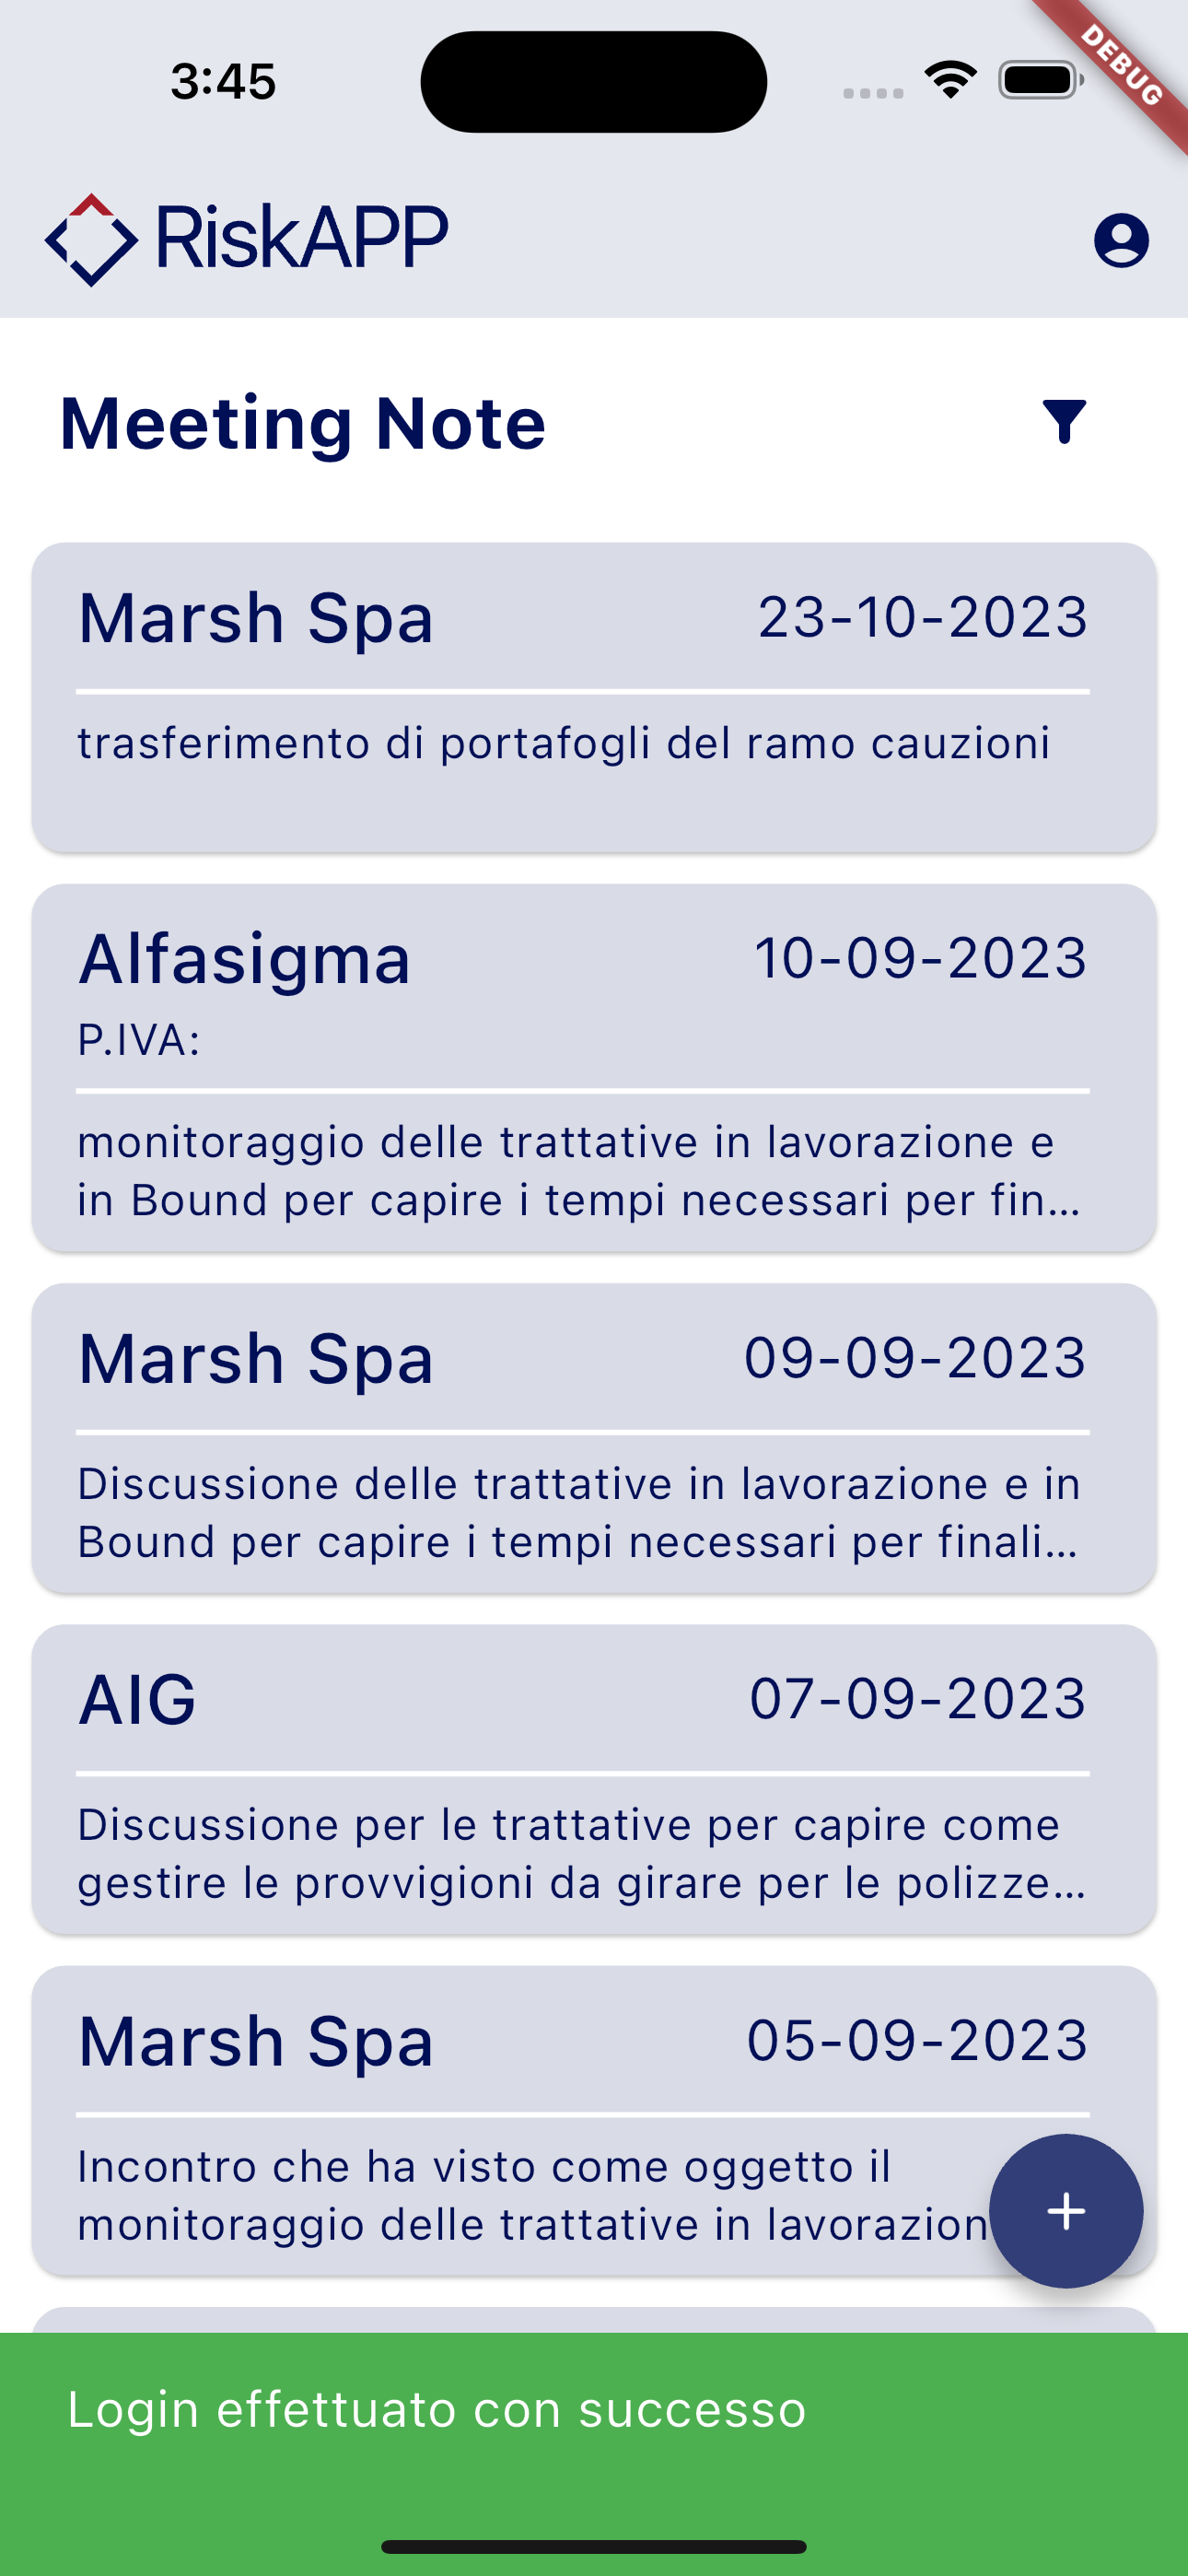
\includegraphics[width=0.3\columnwidth]{screenshot/3-success_snackbar} 
    \hfill
    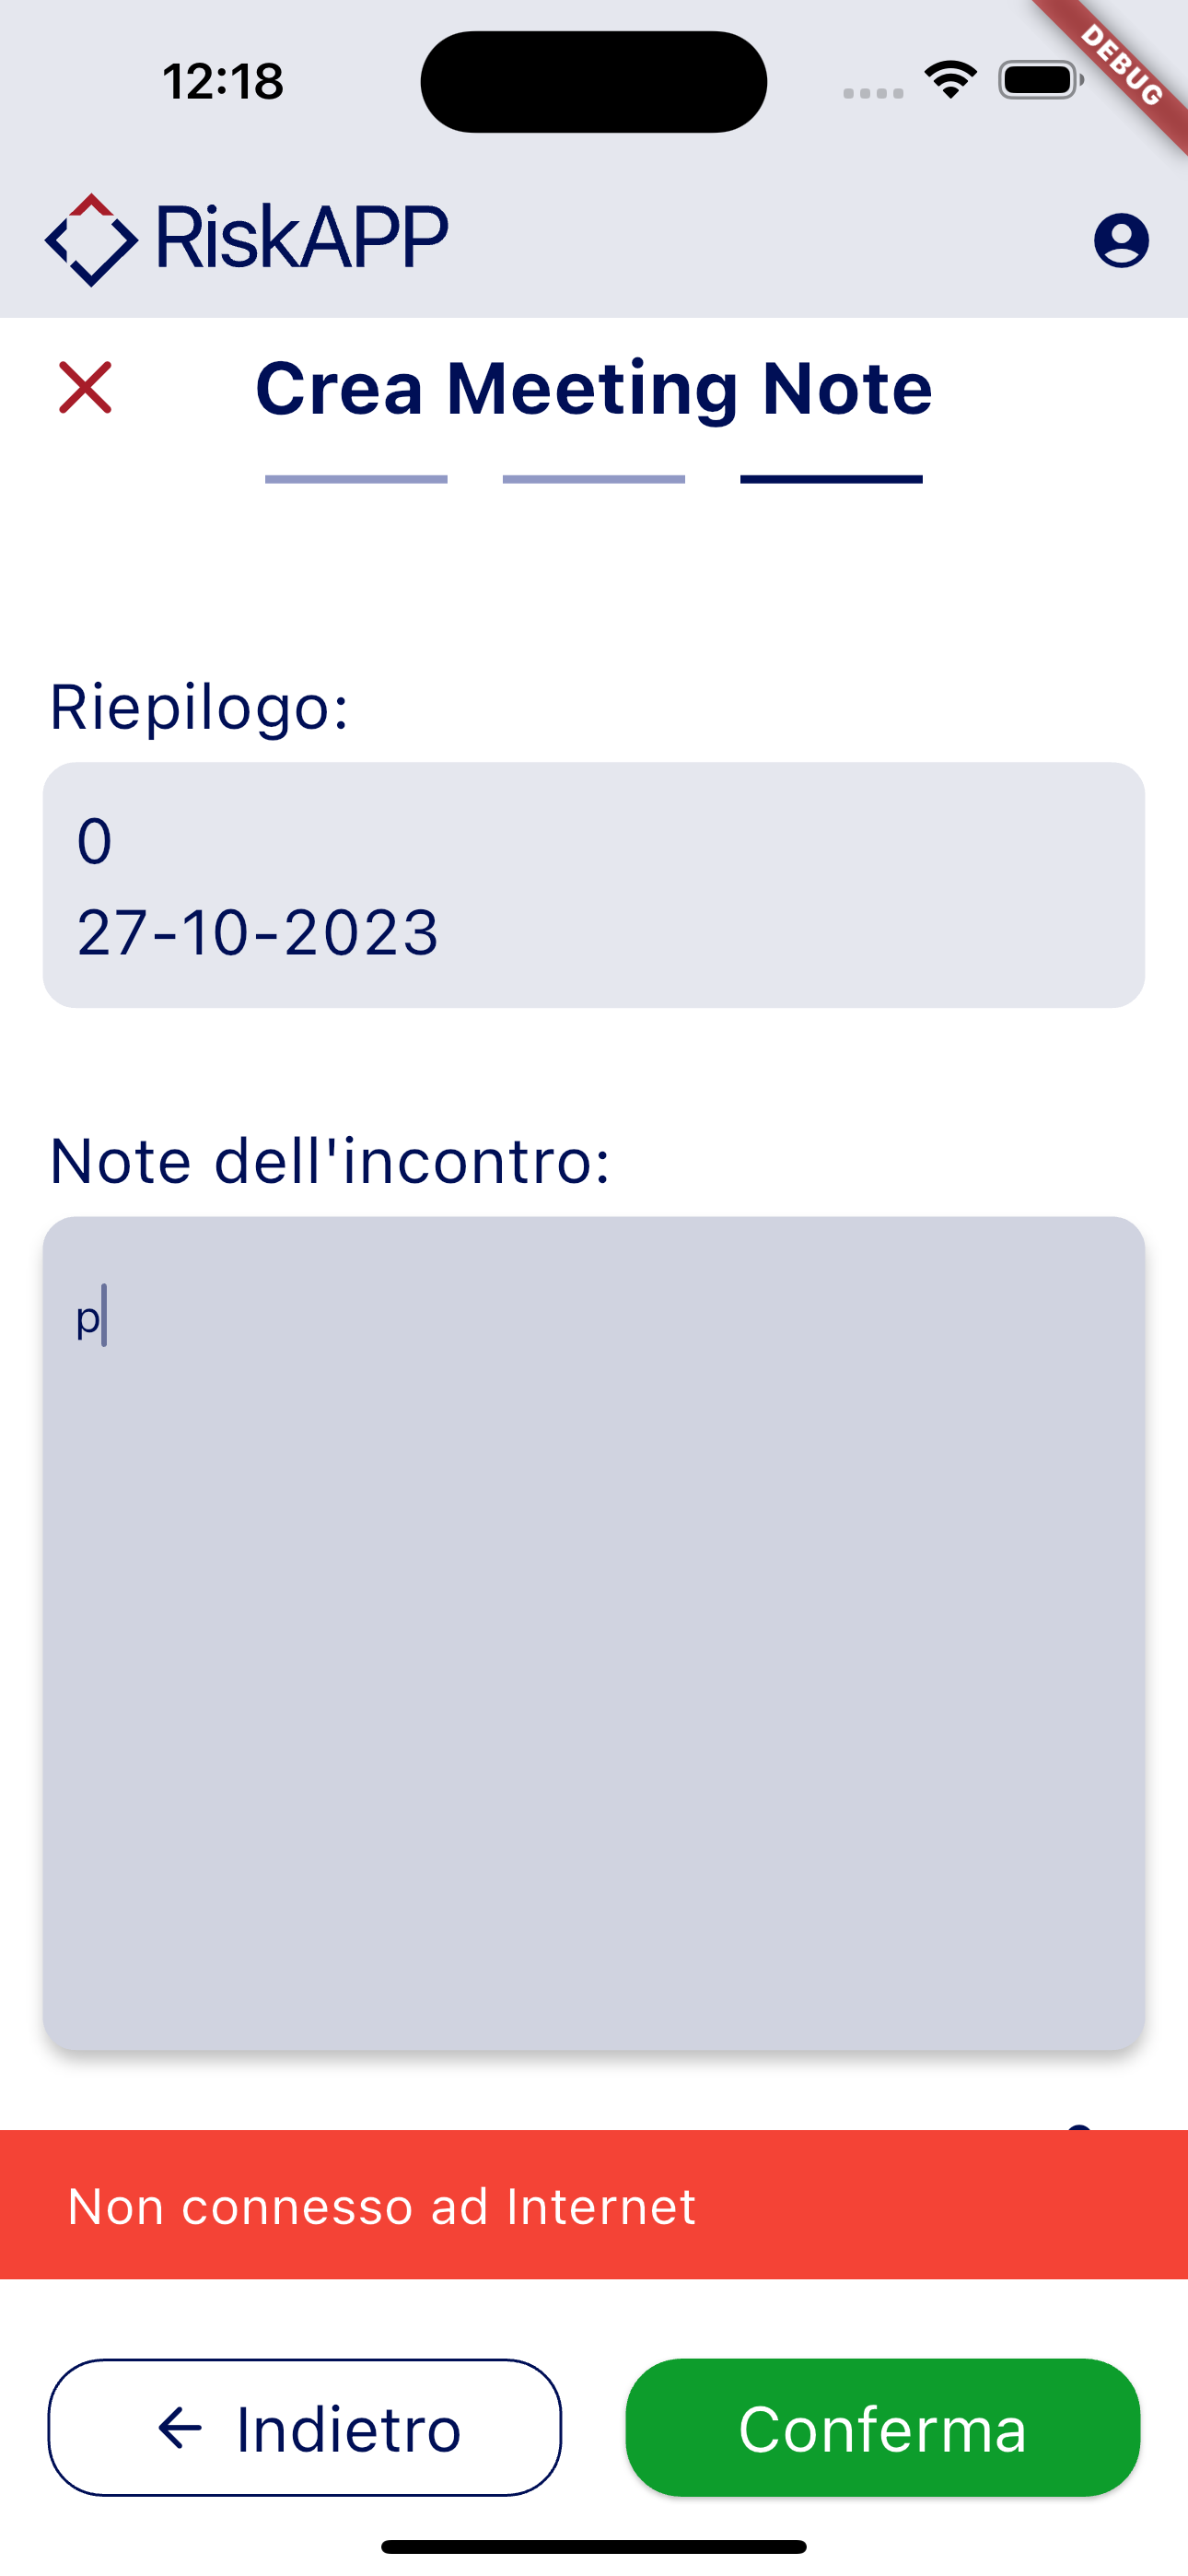
\includegraphics[width=0.3\columnwidth]{screenshot/40-error_snackbar}
    \caption{Esempi di \emph{snackbar}}
    \label{fig:snackbar}
\end{figure}

\newpage

\subsection{Speech to text}
\label{subsec:speech-to-text}

In questo file è presente la classe \lstinline{AudioRecognizer} che implementa la libreria \lstinline{SpeechToText}\cite{site:speech-to-text} per la gestione della dettatura vocale. \\
In essa sono stati definiti i seguenti metodi:
\begin{itemize}
    \item \lstinline{initSpeech}, determina se il dispositivo supporta la dettatura vocale;
    \item \lstinline{startListening}, avvia la dettatura vocale, inoltre vengono impostati alcuni parametri, come la lingua e la durata massima della registrazione;
    \item \lstinline{stopListening}, interrompe la dettatura vocale;
    \item \lstinline{isListening}, restituisce \lstinline{true} se la dettatura vocale è in corso;
\end{itemize}

\section{main.dart}
\label{sec:main}

Il file \lstinline{main.dart} è il punto di ingresso dell'applicazione, in particolare è presente la funzione \lstinline{main} che si occupa di inizializzare l'applicazione, fissando l'orientamento dello schermo a \lstinline{portraitUp} e dichiarando il \lstinline{ProviderScope}. \\
Richiama poi \lstinline{MyApp}, un \emph{ConsumerWidget}, e come prima cosa controlla se è salvato in memoria il \emph{token} di autenticazione attraverso \lstinline{authProvider} (sezione \ref{subsec:authentication-provider}) e decidere se rimandare alla schermata di autenticazione o alla schermata principale dell'applicazione. \\
Il reindirizzamenton avviene attraverso \lstinline{InitApp}, uno \emph{StatelessWidget}, invocando \lstinline{ScreenUtilInit} (sezione \ref{sec:responsivity}), fissando inoltre il parametro \lstinline{supportedLocales} a \lstinline{const Locale('it', 'IT')}, in modo tale che l'applicazione imposti automaticamente alcuni \emph{widget} come il calendario e la data nel formatto corretto e infine viene impostato il tema dell'applicazione (discusso precedentemente).

\section{Responsività}
\label{sec:responsivity}

Per la gestione della responsività dell'applicazione è stata utilizzata la libreria \lstinline{flutter_screenutil}\cite{site:screenutil} che si occupa di adattare le dimensioni degli elementi grafici in base a quelle dello schermo del dispositivo. \\
In particolare è stato invocato \lstinline{ScreenUtilInit} per inizializzare la libreria, fissando il parametro \lstinline{designSize} con le dimensioni definite nel \gls{mockup}\glsoccur, in modo tale che la libreria possa mantenere le proporzioni degli elementi grafici. 

\section{Usabilità}
\label{sec:usability}

% \section{Icona}
% \label{sec:icon}

\section{Ottimizzazioni per le performance}
\label{sec:performance}



% Listato delle varie classi principali implementate
% Fai riferimento allo storico dei commits su GitHub

% \section{Design Pattern utilizzati}

    % \chapter{Documentazione}
\label{cap:documentazione}

% \intro{In questo capitolo viene descritto }\\

\section{README}
\label{sec:readme}

Insieme al codice sorgente dell'applicazione è stata consegnata anche una breve documentazione, scritta in lingua inglese, secondo la richiesta dell'azienda, utilizzando il linguaggio di markup \gls{markdown}\glsoccur.\\
È stato redatto il file \lstinline{README.md}, il cui contenuto è riportato di seguito:
\begin{itemize}
    \item \textbf{Abstract}: breve descrizione dell'applicazione e del contesto applicativo;
    \item \textbf{Getting Started}: istruzioni per poter compilare ed eseguire l'applicazione;
    \item \textbf{Libraries Used}: elenco delle librerie utilizzate, necessarie per la compilazione;
    \item \textbf{Project Structure}: descrizione della struttura e architettura del progetto;
    \item \textbf{Features}: elenco delle funzionalità implementate.
\end{itemize}

\lstset{
    language=Java,
    basicstyle=\ttfamily,
    keywordstyle=\color{blue}\ttfamily,
    stringstyle=\color{red}\ttfamily,
    commentstyle=\color{green!60!black}\ttfamily,
}

\section{Documentazione del codice}
\label{sec:documentazione-codice}

Per quanto riguarda il codice sorgente, è stato scritto un commento per ogni classe, metodo e variabile, in modo da rendere più chiara la lettura del codice.\\
Lo standard seguito è quello proposto nella documentazione ufficiale di \emph{Dart}\cite{site:comment}. \\

In particolare, per i commenti alle classi, è stato utilizzato il seguente formato, spiegando anche il significato e scopo delle variabili di stato:
\begin{lstlisting}[language=Java, caption={Commento classe}, captionpos=b]
/// Class encapsulating the authentication's params,
/// given in input to the authentication request.
///
/// [_username], the user's username
///
/// [_password], the user's password
class AuthArgs {
    final String _username;
    final String _password;
    // ...
}
\end{lstlisting}

Per i commenti ai metodi, è stato utilizzato il medesimo formato utilizzato per i commenti alle classi, spiegando lo scopo del metodo, i parametri in input e il valore di ritorno:
\begin{lstlisting}[language=Java, caption={Commento metodo}, captionpos=b]
/// Authenticate the user with the given authentication [args]
/// retrieving the token and saving it in the local storage if the authentication request is successful.
///
/// Return [AuthResponse] object with:
///
/// - [AuthValues] object, containing the token if the request is successful
///
/// - [StatusResponse] object, containing the response's status
Future<AuthResponse> authenticate({required AuthArgs args}) async {
    log("credentials: ${args.toString()}");

    // ...

    log("auth response: ${result.toString()}");

    // ...
}
\end{lstlisting}
    \chapter{Conclusioni}
\label{cap:conclusioni}

\intro{In questo ultimo capitolo verranno illustrati gli obiettivi raggiunti, il consuntivo delle attività e infine verrà fornita una valutazione personale sul tirocinio svolto.}\\

\section{Obiettivi raggiunti}
\label{sec:raggiungimento-obiettivi}

La Tabella \ref{tab:obbiettivi-raggiunti} illustra gli obiettivi raggiunti al termine del tirocinio.

\begin{table}
    \centering
    \begin{tabular}{|l|l|l|}
        \hline
        \textbf{Obiettivo} & \textbf{Priorità} & \textbf{Stato} \\ \hline
        \hyperref[O01]{O01}                & Obbligatorio      & Soddisfatto    \\ \hline
        \hyperref[O02]{O02}                & Obbligatorio      & Soddisfatto    \\ \hline
        \hyperref[O03]{O03}                & Obbligatorio      & Soddisfatto    \\ \hline
        \hyperref[O04]{O04}                & Obbligatorio      & Soddisfatto    \\ \hline
        \hyperref[O05]{O05}                & Obbligatorio      & Soddisfatto    \\ \hline
        \hyperref[D01]{D01}                & Obbligatorio      & Soddisfatto    \\ \hline
        \hyperref[D02]{D02}                & Obbligatorio      & Non soddisfatto    \\ \hline
        \hyperref[F01]{F01}                & Obbligatorio      & Non soddisfatto    \\ \hline
    \end{tabular}%
\caption{Tabella con gli obiettivi raggiunti}
\label{tab:obbiettivi-raggiunti}
\end{table}

\noindent Il mancato soddisfascimento degli obiettivi \emph{D02} e \emph{F01}, ovvero il \emph{deploy} e la stesura dei test per la verifica e validazione dell'applicazione, è stato causato principalmente dalla mancanza di tempo. \\
Come evidenziato dal reale svolgimento delle attività (Sezione \ref{subsec:variazione-pianificazione}), la fase di sviluppo è stata più lunga del previsto.\\
Malgrado non siano stati progettati e scritti i test per la verifica e validazione dell'applicazione, si è comunque cercato di mantenere un codice pulito e ben strutturato, in modo da facilitare eventuali modifiche e manutenzioni future, anche se come garanzia di qualità non può considerarsi sufficiente.
Si specifica, inoltre, che la verifica delle funzionalità dell'applicazione è stata effettuata dal tutor aziendale o da altri colleghi, lungo tutto il periodo di sviluppo del progetto, fornendo un \emph{feedback} immediato, permettendo così di apportare eventuali modifiche correttive e miglioramenti.\\
Per quanto riguarda il \gls{deploy}\glsoccur, il principale motivo per cui non è stato effettuato, è da imputarsi al fatto che l'utenza a cui è rivolta l'applicazione è molto ristretta, risultava quindi superfluo e non necessario pubblicarla sulle piattaforme \emph{Google Play Store} e \emph{Apple App Store}. Tale decisione è stata presa dal tutor aziendale che ha ritenuto più opportuno pensare ad un modo alternativo per distribuire l'applicazione direttamente agli utenti finali.

\section{Consuntivo delle attività}
\label{sec:consultivo-attivita}

Sulla base di quanto descritto nella Sezione \ref{sec:raggiungimento-obiettivi}, la Tabella \ref{tab:consultivo-ore} riporta la differenza tra le ore pianificate (presenti nel documento \emph{Piano di lavoro}) ed effettive per ogni attività del tirocinio.

\begin{table}
    \centering
    \begin{tabularx}{\textwidth}{|c|c|X|}
        \hline
        \textbf{Ore effettive} & \textbf{Ore pianificate} & \textbf{Descrizione dell'attività} \\\hline
        
        \textbf{70} & \textbf{80} & \textbf{Formazione sulle tecnologie} \\	 
        \hline
        
        \textbf{40} & \textbf{40} & \textbf{Definizione architettura di riferimento e relativa documentazione} \\ \hdashline 
        \multirow{3}{0cm}\\ 
        \textit{14} &
        \textit{12} & 
        \textit{Analisi del problema e del dominio applicativo} \\
        \textit{20} &
        \textit{22} & 
        \textit{Progettazione della piattaforma e relativi test} \\
        \textit{6} &
        \textit{6} & 
        \textit{Stesura documentazione relativa ad analisi e progettazione} \\
        \hline
        

        \textbf{192} & \textbf{160} & \textbf{Sviluppo}  \\ \hdashline 
        \multirow{5}{0cm}\\ 
        \textit{40} &
        \textit{26} & 
        \textit{Implementazione del meccanismo di autenticazione e integrazione con il sistema preesistente per il prelevamento dei dati da visualizzare nell'applicazione} \\
        \textit{40} &
        \textit{34} & 
        \textit{Implementazione delle funzionalità di creazione e compilazione (testuale e vocale) delle meeting-note} \\
        \textit{40} &
        \textit{28} & 
        \textit{Integrazione del servizio OpenAI} \\
        \textit{24} &
        \textit{40} & 
        \textit{Attività di testing} \\
        \textit{48} &
        \textit{32} & 
        \textit{Sviluppo UI} \\
        \hline
        
        \textbf{10} & \textbf{40} & \textbf{Verifica e Validazione finale}  \\ \hdashline 
        \multirow{3}{0cm}\\ 
        \textit{0} &
        \textit{24} & 
        \textit{Esecuzione dei test per la verifica e collaudo dell'applicazione} \\
        \textit{10} &
        \textit{8} & 
        \textit{Stesura documentazione finale} \\
        \textit{0} &
        \textit{8} & 
        \textit{Deploy dell'applicazione} \\
        \hline
        
        \textbf{Totale ore} & \multicolumn{1}{|X|}{\textbf{312}} \\ 
        \hline
        
    \end{tabularx}
    \caption{Consuntivo della durata delle attività}
    \label{tab:consultivo-ore}
\end{table}

\section{Valutazione personale}
\label{sec:valutazione-personale}

Il tirocinio è stato un'esperienza molto formativa, in quanto mi ha permesso di mettere in pratica le conoscenze e metodologie acquisite durante il percorso di studi in un contesto lavorativo.\\
Come già menzionato in precedenza, nonostante la mia familiarità con alcune delle tecnologie adottate, ho avuto modo di approfondirle e di imparare nuovi concetti, soprattutto per quanto riguarda il \emph{framework} \emph{Flutter}.\\
Inoltre, per la prima volta ho avuto modo di lavorare ad un progetto in maniera più professionale, seguendo anche alcuni principi affrontati durante il corso di \emph{Ingegneria del Software}, come ad esempio la pianificazione della fase di sviluppo, fissando delle \gls{milestone}\glsoccur, mantenendo traccia dei progressi per il raggiungimento degli obiettivi del progetto, e la documentazione del codice, in modo da rendere più facile la comprensione e la manutenzione del codice.\\  
L'azienda mi ha lasciato molta autonomia durante lo sviluppo del progetto e mi ha fornito un \emph{feedback} costante, permettendomi di migliorare e di imparare nuove cose. \\
In conclusione, ritengo che il tirocinio sia stato un'esperienza molto positiva, che mi ha permesso di crescere sia dal punto di vista professionale che personale.

    \appendix
    % \chapter{Appendice A}

\epigraph{Citazione}{Autore della citazione}
}

    \backmatter
    \printglossary[type=\acronymtype, title=Acronimi, toctitle=Acronimi]
    \printglossary[type=main, title=Glossario, toctitle=Glossario]

    \cleardoublepage
\chapter{Bibliografia}

% \nocite{*}

% Print book bibliography
\printbibliography[heading=subbibliography,title={Riferimenti bibliografici},type=book]

% Print site bibliography
\printbibliography[heading=subbibliography,title={Siti web consultati},type=online]

\end{document}
